\documentclass[  10pt, twoside]{report} %draft ,
% LTeX: enabled=false
\usepackage{natbib}
\usepackage[nottoc, notlot, notlof]{tocbibind}
\usepackage[a4paper, tmargin=2.5cm, bmargin=2.5cm,lmargin=2.5cm, rmargin=2.5cm, includefoot] {geometry} % 
\usepackage{fancyhdr}
\usepackage{lastpage}
\usepackage{svg}
\usepackage{caption} %[font=footnotesize]
\usepackage{graphicx}
\usepackage{pdfpages}
\usepackage{subcaption}
\usepackage{color,soul}
\usepackage{wrapfig}
\usepackage{subcaption}
\usepackage{amsmath}
\numberwithin{equation}{chapter}
\usepackage{physics}
\usepackage{mathrsfs}
\usepackage{tabularx}
\usepackage{multirow}
\usepackage{multicol}
\usepackage{xurl}
\usepackage{amssymb}
\usepackage{hyperref}
\hypersetup{colorlinks=true,linkcolor=black,citecolor=black,urlcolor=cyan,pdfpagelayout=TwoPageRight,pdftitle={Development of Control Strategies for Earthquake Reproduction on Shaking Platform}, pdfauthor={Afonso Costa Henrique},pdfsubject={Development of Control Strategies for Earthquake Reproduction on Shaking Platform}}
\usepackage[dvipsnames]{xcolor}
\usepackage{enumitem}
% \usepackage{listings}
% \usepackage{matlab-prettifier}
\usepackage{float}
\usepackage{silence}
\WarningFilter{caption}{Unused}
\WarningFilter{hyperref}{Draft mode on}
\newcommand{\mycomment}[1]{}
\usepackage{arydshln}
\usepackage[english]{babel}
\usepackage{cases}

\usepackage{titlesec}
\titleformat{\chapter}[display]
 {\normalfont\huge\bfseries\linespread{0.85}\selectfont} %\hyphenpenalty=10000\exhyphenpenalty=10000
  {\chaptertitlename\ \thechapter}
  {10pt}
  {\Huge}
\titlespacing*{\chapter}{0pt}{-10pt}{10pt}

\setcounter{tocdepth}{3}
\setcounter{secnumdepth}{5}
\titleformat{\subsubsection}{\normalfont\normalsize\bfseries}{\thesubsubsection}{1em}{}
\titlespacing*{\subsubsection}{0pt}{3.25ex plus 1ex minus .2ex}{1.5ex plus .2ex}

% paragraph — uses letters
\renewcommand{\theparagraph}{\thesubsubsection.\alph{paragraph}}
\titleformat{\paragraph}{\normalfont\normalsize\bfseries}{\theparagraph}{1em}{}
\titlespacing*{\paragraph}{0pt}{3.25ex plus 1ex minus .2ex}{1.5ex plus .2ex}

\let\oldsection\chapter
\renewcommand{\chapter}{\cleardoublepage\oldsection}

\usepackage{indentfirst}

\usepackage{tikz}
\usetikzlibrary{patterns,decorations.pathmorphing,positioning,arrows.meta, positioning, shapes.multipart, calc,arrows, positioning, calc, shapes.geometric}
%% ----- FONT SELECTION -----
\usepackage[nopatch=footnote]{microtype}   % fine-tunes spacing to avoid overflows
% \usepackage{lmodern}     % improved CM Roman
\renewcommand{\rmdefault}{phv}
\renewcommand{\sfdefault}{phv}

%% ----------  Packages above --------
% Define a simple centered-number style (put this in your preamble)
\fancypagestyle{plainroman}{
  \fancyhf{}                          % clear all
  \fancyfoot[C]{\thepage}            % just the page number, centered
  \renewcommand{\headrulewidth}{0pt} % no header line
}

\usepackage{setspace}
\onehalfspacing
\AtBeginEnvironment{minipage}{\renewcommand{\baselinestretch}{1.5}\normalsize}

\AtBeginEnvironment{itemize}{\onehalfspacing}
\AtEndEnvironment{itemize}{\onehalfspacing}
 
\usepackage{nomencl} %%%%%%%%    NOMENCLATURE  %%%%%%%%     NOMENCLATURE     %%%%%%%%   NOMENCLATURE  %%%%%%%% 
\makenomenclature
\nomenclature{$\star$}{Convolution} 
\nomenclature{$(\cdot)^{*}$}{Complex Conjugate}
\nomenclature{$(\cdot)^{\intercal}$}{Transpose}
\nomenclature{$f_i$}{Frequency of mode \textit{i}}
\nomenclature{$\xi_i$}{Damping coefficient of mode \textit{i}}
\nomenclature{$E$}{Expected value} 
\nomenclature{$R_x$}{Auto covariance of signal $x$} 
\nomenclature{$R_{yx}$}{Cross covariance of signals $y$ }
\nomenclature{$\Phi_x$}{Auto spectral density of signal $x$} 
\nomenclature{$\Phi_{yx}$}{Cross spectral density of signals $y$ and $x$} 
\nomenclature{$C$}{Controller} 
\nomenclature{$G_0$}{Input-Output system} 
\nomenclature{$S_0$}{Sensitivity function} 
\nomenclature{$H_0$}{Noise filter in system} 
\nomenclature{$\omega$}{Frequency} 
\nomenclature{$T_s$}{Sampling time} 
\nomenclature{$u$}{Input signal} 
\nomenclature{$v$}{Additive output disturbance} 
\nomenclature{$y$}{Output signal}




\usepackage[acronym,nonumberlist,nopostdot,nogroupskip]{glossaries}
\setglossarystyle{list}
\renewcommand{\glsnamefont}[1]{\textbf{#1}}  %%%%%%%%   GLOSSARY  %%%%%%%%     
\makeglossaries
\newacronym{LNEC}{LNEC}{Laboratório Nacional de Engenharia Civil}
\newacronym{MSE}{MSE}{Mean squared error}
\newacronym{ST1D}{ST1D}{Uniaxial shaking table}
\newacronym{ST3D}{ST3D}{Triaxial shaking table}
\newacronym{1DOF}{1DOF}{One degree-of-freedom}
\newacronym{2DOF}{2DOF}{Two degree-of-freedom}
\newacronym{PBSD}{PBSD}{Performance-Based Seismic Design}
\newacronym{RTHS}{RTHS}{Real-time hybrid simulation}
\newacronym{PID}{PID}{Proportional-Integral-Derivative}
\newacronym{ATTC}{ATTC}{Acceleration Trajectory Tracking Control}
\newacronym{ADRC}{ADRC}{Active disturbance rejection control}
\newacronym{AMSE}{AMSE}{Adaptive model-based state estimators }
\newacronym{ESO}{ESO}{Extended state observer}
\newacronym{PD}{PD}{Proportional-derivative}
\newacronym{AIC}{AIC}{Adaptive inverse control}
\newacronym{OIC}{OIC}{offline inverse model compensator}
\newacronym{TVC}{TVC}{Three-Variable Control}
\newacronym{AHC}{AHC}{Adaptive Harmonic Cancellation}
\newacronym{APC}{APC}{Amplitude/Phase Control}
\newacronym{OLI}{OLI}{Online Iteration}
\newacronym{LTI}{LTI}{Linear time-invariant}
\newacronym{PID-F}{PID-F}{Proportional integral filtered derivative}
\newacronym{LQI}{LQI}{Linear quadratic integral}
\newacronym{LQR}{LQR}{Linear quadratic regulator}
\newacronym{LQG}{LQG}{Linear quadratic guassian}
% \newacronym{OLI}{OLI}{Online}
% \newacronym{OLI}{OLI}{Online}
% \newacronym{OLI}{OLI}{Online}
% \newacronym{OLI}{OLI}{Online}
% \newacronym{OLI}{OLI}{Online}
% \newacronym{OLI}{OLI}{Online}
% \newacronym{OLI}{OLI}{Online}
% \newacronym{OLI}{OLI}{Online}







\raggedbottom
%%%%%%%%%%%%%%%%%%%%%%%%%%%%%%%%%%%%%%%%%%%%%%%%%%%%%%%%%%%%%%%%%%%%%%%%%%%%%%%%%%%%%%%%%
\begin{document}
\begin{titlepage} % CAPA
\thispagestyle {empty}

\hspace{15mm}
\includegraphics[bb=7.0cm 7.5cm 0cm 0cm,scale=0.23]{Figures/Tecnico_ID_Principal_RBG-COR.png}

\centering

\vspace{2.5cm}

\fbox{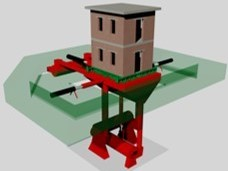
\includegraphics[width=0.4\textwidth]{Intro/Triaxial_with_2floor.jpg}}  

\vspace{5mm} 


\LARGE\textbf{ Development of Control Strategies for Earthquake Reproduction on Shaking Platform}

\vspace{5mm} 

\Large \textbf{Afonso Costa Henrique} \par

\vspace{5mm}

\large Thesis to obtain the Master of Science Degree in \par
\LARGE \textbf{Mechanical Engineering} \par

\vspace{5mm}

\large
\begin{tabular}{l l}
  Supervisors:& Miguel Ayala Botto \\
              &Fernando Pires de Oliveira
\end{tabular}

\vspace{5mm}

\Large \textbf{Examination Committee}

\vspace{2mm}

\large
\begin{tabular}{r l}
  Chairperson: & Lorem Ipsum \\
  Supervisor: & Dolor Sit Amet \\
  Members of the Committee: & Consectetur Adipiscing Elit \\
                       & Maecenas Feugiat \\
                       & Sapien Libero
\end{tabular}
\vfill
\Large \textbf{May 2026} \par

\end{titlepage}
\pagenumbering{Roman}
\setcounter{page}{2}
\clearpage
%%%%%%%%%%%%%%%%%%%%%%%%%%%%%%%%%%%%%%%%%%%%%%%%%%%%%%%%%%%%%%%%%%%%%%%%%%%%%%%%%%%%%%%%%
\pagestyle{plainroman}

\newpage
\mbox{}
\newpage
%%%%%%%%%%%%%%%%%%%%%%%%%%%%%%%%%%%%%%%%%%%%%%%%%%%%%%%%%%%%%%%%%%%%%%%%%%%%%%%%%%%%%%%%%
\normalsize

% Dedicatoria


\begin{flushright}

\vspace*{\fill} % pushes following text to bottom
% Ao professor Miguel Botto e ao Fernando Oliveira,\\ % que me trouxeram a este projeto e sempre me guiaram

% Ao António Correia, \\%pela 

% Ao Paulo Candeias, \\ %um poço de conhecimento e uma ajuda indispensável
% \vspace{5mm}

Aos meus pais, que me deram a possibilidade de estudar,


Eternamente grato
\vspace*{\fill}
\end{flushright}
\clearpage

%%%%%%%%%%%%%%%%%%%%%%%%%%%%%%%%%%%%%%%%%%%%%%%%%%%%%%%%%%%%%%%%%%%%%%%%%%%%%%%%%%%%%%%%%
\newpage
\mbox{}
\newpage
%%%%%%%%%%%%%%%%%%%%%%%%%%%%%%%%%%%%%%%%%%%%%%%%%%%%%%%%%%%%%%%%%%%%%%%%%%%%%%%%%%%%%%%%%
\null\vskip5cm%
\begin{flushleft}
Declaration

I declare that this document is an original work of my own authorship and that it fulfills all the requirements of the Code of Conduct and Good Practices of the Universidade de Lisboa.
\end{flushleft}
\vfill\newpage

%%%%%%%%%%%%%%%%%%%%%%%%%%%%%%%%%%%%%%%%%%%%%%%%%%%%%%%%%%%%%%%%%%%%%%%%%%%%%%%%%%%%%%%%%
\newpage
\mbox{}
\newpage
%%%%%%%%%%%%%%%%%%%%%%%%%%%%%%%%%%%%%%%%%%%%%%%%%%%%%%%%%%%%%%%%%%%%%%%%%%%%%%%%%%%%%%%%%
\section*{Acknowledgments}
\addcontentsline{toc}{section}{Acknowledgments}% Add entry in the table of contents as section

A few words about the university, financial support, research advisor, dissertation readers, faculty or other professors, lab mates, other friends and family...

%%%%%%%%%%%%%%%%%%%%%%%%%%%%%%%%%%%%%%%%%%%%%%%%%%%%%%%%%%%%%%%%%%%%%%%%%%%%%%%%%%%%%%%%%
\newpage
\mbox{}
\newpage
%%%%%%%%%%%%%%%%%%%%%%%%%%%%%%%%%%%%%%%%%%%%%%%%%%%%%%%%%%%%%%%%%%%%%%%%%%%%%%%%%%%%%%%%%


\begin{otherlanguage}{portuguese}
\section*{Resumo}
\addcontentsline{toc}{section}{Resumo}% Add entry in the table of contents as section

No domínio científico da engenharia sísmica, não obstante os avanços verificados em simulação computacional, persistem limitações na modelação precisa de comportamentos estruturais complexos, não lineares, ou de outras dinâmicas insuficientemente estudadas. As simulações numéricas, mesmo quando baseadas em métodos avançados, requerem dados experimentais para validar os modelos matemáticos e garantir uma precisão adequada. Além disso, as abordagens de aprendizagem automática também dependem de dados experimentais para o treino e atualização de modelos. Os ensaios experimentais constituem assim um meio indispensável à validação e calibração desses modelos. Nessa linha, os ensaios experimentais em engenharia sísmica continuam a ser indispensáveis para validar modelos, compreender comportamentos estruturais complexos e garantir a segurança estrutural.

Nesta tese, um modelo computacional da plataforma sísmica uniaxial do LNEC é utilizado para comparar o desempenho, em termos de espetro de resposta, de três estratégias de controlo distintas: 1) o método iterativo atualmente utilizado, designado por OLI, que consiste num controlo pseudo-adaptativo offline em anel aberto com o ensaio a decorrer em anel fechado com um controlador PI (proporcional-integral); 2) um controlador sintonizado PID-F (proporcional-integral-derivativo-filtrado); 3) um controlador ótimo de formulação linear-quadrática-integral (LQI).

Adicionalmente, para a sintonização dos controladores, é proposto um método de identificação adequado para sistemas que operam exclusivamente em anel fechado, como é o caso das mesas sísmicas do LNEC. Este método é aplicado na identificação de um agitador eletrodinâmico, sendo o modelo identificado posteriormente utilizado numa avaliação e comparação do desempenho das três estratégias de controlo. Adicionalmente, para o controlador LQI, é implementado um processo de otimização dos parâmetros da função de custo.

Os resultados indicam que ambos os controladores, PID-F e LQI, oferecem desempenho superior comparativamente ao método OLI, sendo o controlador LQI aquele que apresenta melhor desempenho em todas as simulações, revelando-se assim o mais promissor para aplicação no controlo das plataformas sísmicas avaliadas.

\vfill

\textbf{Palavras-chave:} Engenharia Sísmica, Controlo de Sistemas, Identificação de Sistemas, Identificação em Anel Fechado
\end{otherlanguage}
%%%%%
% LTeX: enabled=true
\clearpage
\section*{Abstract}
\addcontentsline{toc}{section}{Abstract}% Add entry in the table of contents as section

Despite computational models employed in earthquake simulations having attained a high degree of sophistication and reliability, they continue to face significant limitations when complex, nonlinear, or insufficiently understood structural behaviours are considered. Moreover, numerical simulations, even when based on advanced methods, require experimental benchmarks to ensure accuracy, and machine learning approaches equally rely on experimental data for training and updating models. Experimental testing thus provides critical validation and calibration for these models. To this end, experimental testing in earthquake engineering remains indispensable for model validation, the understanding of complex structural behaviours, and the assurance of structural safety.

This thesis analyses control strategies for reproducing earthquake ground motion on the uniaxial shaking table located at the Laboratório Nacional de Engenharia Civil, by means of a computational model of the system. The objective of the controller is to ensure that the shaking table reproduces the target earthquake ground motion as accurately as possible. The overall performance is evaluated in terms of response spectra for three distinct control strategies: 1) the currently employed OLI method, consisting of a pseudo-open-loop offline adaptive control with an iterative process of generating drive signals and conducting the tests in closed loop with a PI controller; 2) a tuned PID-F controller (proportional, integral, and filtered derivative); and 3) an LQI controller.

Additionally, in order to tune the controllers, an identification method more appropriate for systems operating exclusively under closed-loop conditions, such as LNEC's shaking tables, is proposed. This method is subsequently applied to the identification of an electrodynamic shaker, whose identified model is then used to compare the performance of the three control strategies.

The results indicate that both the PID-F and the LQI controllers offer superior performance compared to the OLI method, with the optimal controller yielding the best overall performance and being considered the most promising solution for the control of the studied shaking tables.

\vfill

\textbf{Keywords:} : Earthquake Engineering, Control Systems, System Identification, Closed-loop Identification

%%%%%%%%%%%%%%%%%%%%%%%%%%%%%%%%%%%%%%%%%%%%%%%%%%%%%%%%%%%%%%%%%%%%%%%%%%%%%%%%%%%%%%%%%
\cleardoublepage 
\tableofcontents % Indice

\cleardoublepage 
\phantomsection
\addcontentsline{toc}{section}{List of Tables}
\listoftables % Tabelas

%\cleardoublepage 
\phantomsection
\addcontentsline{toc}{section}{List of Figures}
\listoffigures %Figuras

%%%%%%%%%%%%%%%%%%%%%%%%%%%%%%%%%%%%%%%%%%%%%%%%%%%%%%%%%%%%%%%%%%%%%%%%%%%%%%%%%%%%%%%%%

\clearpage
\phantomsection
\addcontentsline{toc}{section}{Nomenclature}
\printnomenclature


\clearpage
\phantomsection
%\addcontentsline{toc}{section}{Glossary}% Add entry in the table of contents as section
\glsaddall
\printglossary[type=\acronymtype,title=\acronymname, toctitle=\acronymname]



%\clearpage
\pagestyle{plain}% Apply the general page style to all pages by default
\pagenumbering{arabic}
\chapter{Introduction}

Shaking-table tests consist of mounting a physical model on a stiff platform that is driven so as to reproduce the desired ground-motion time history (reference signal). This experimental technique was introduced in the 1940s and became widespread during the 1960s. Early systems relied on mechanical profiled cams to generate the excitation, but servo-hydraulic systems soon became the standard solution \citep{williams2001,carvalho1998,candeias2023}. 

At the Laboratório Nacional de Engenharia Civil (LNEC) a Goodmans model VG-108 electrodynamic shaker attached to a movable table was installed in the 60s to perform seismic tests \citep{emilio1989}. A uniaxial shaking table (ST1D), shown in figure \ref{fig_3D_render_uniaxial}, was developed and installed, consisting of a 3 m x 2 m horizontal steel platform and a vertical platform body driven by a hydraulic actuator supplied by a dedicated oil-hydraulic circuit \citep{bairao1998,castro1978}. During this period, adaptive control strategies were developed, implemented, and validated both on a small scale shaking table and on the ST1D, for tracking reference earthquake spectrum (frequency domain), iteratively \citep{carvalhal1974,carvalhal1979}. Increasingly demanding requirements for reproducing seismic excitation along all three directions motivated the development of the triaxial shaking table (ST3D), shown in figure \ref{fig_3D_render_triaxial}, which has been installed and operational at LNEC since the mid-1990s \citep{emilio1989}.

%\vspace{-10mm}

\begin{figure}[H]
\begin{minipage}[t]{0.49\textwidth}
    \centering
    \fbox{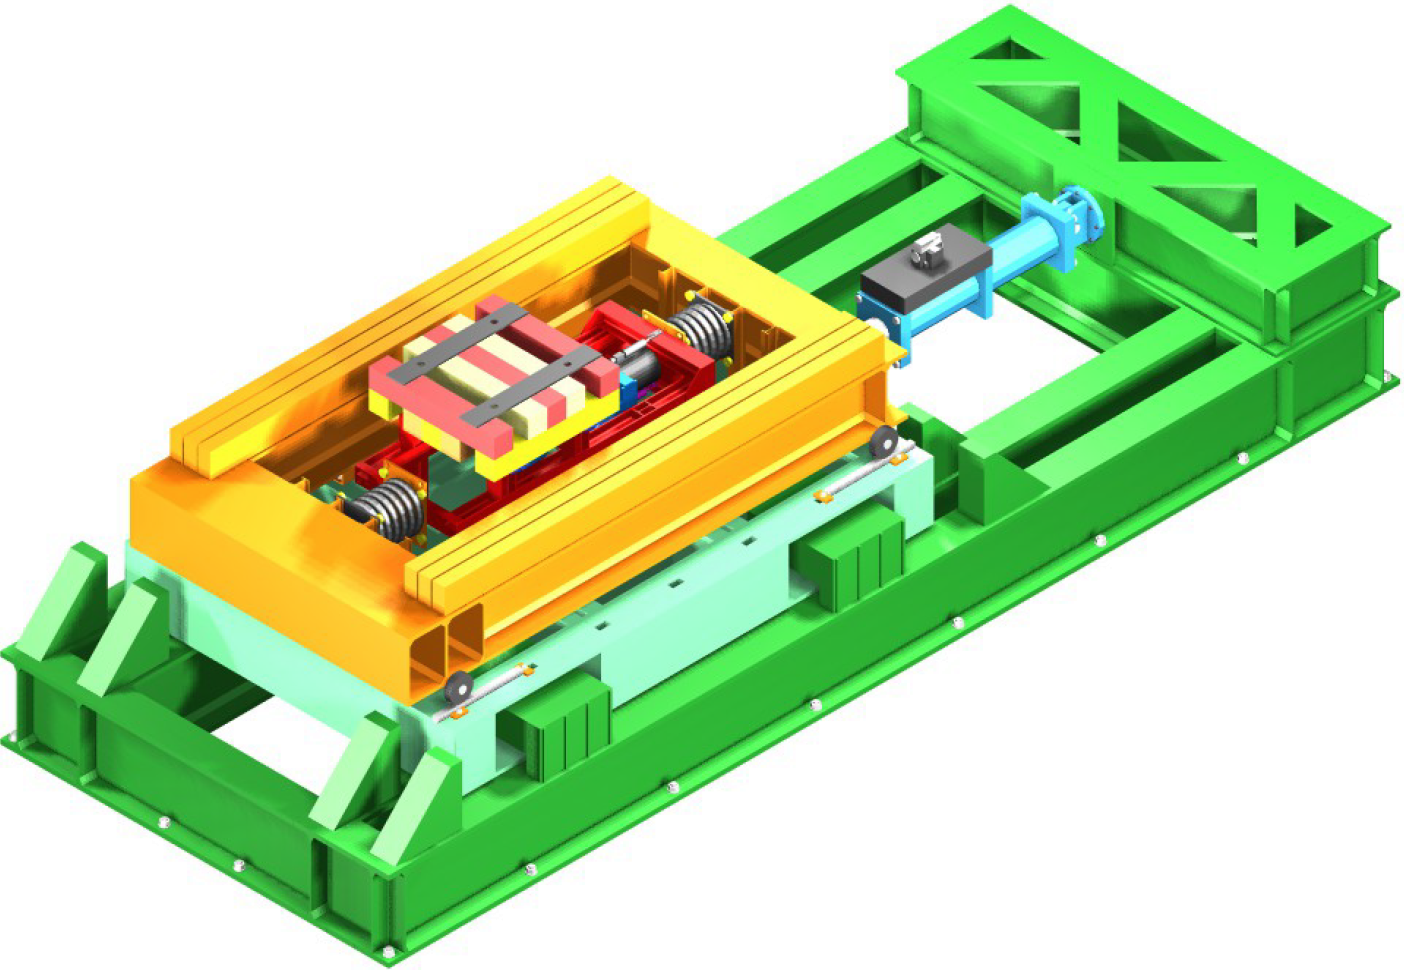
\includegraphics[width=0.97\textwidth]{Figures/capa.png}}
    \caption{A 3D rendering of LNEC's uniaxial shaking table with a coupled 2DOF system (red and orange carts). The platen is shown in light green, and the actuators in blue.}
    \label{fig_3D_render_uniaxial}
\end{minipage}
\hfill
\begin{minipage}[t]{0.49\textwidth}
    \centering
    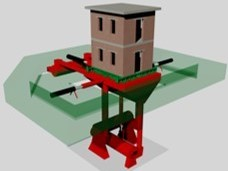
\includegraphics[width=\textwidth]{Intro/Triaxial_with_2floor.jpg}
    \caption{A 3D rendering of LNEC's triaxial shaking table with a scaled test specimen of a two-story building. The rigid elements (platen and linkages) are shown in red, and the actuators in black and silver.}
    \label{fig_3D_render_triaxial}
\end{minipage}
\end{figure}

\clearpage
\section{Seismic Platform  Tests at LNEC}

The current seismic platform testing process at Laboratório Nacional de Engenharia Civil (LNEC) consists of iteratively synthesizing a drive signal, distinct from the reference signal, so that the platform replicates the response spectra of the reference signal, i.e. the earthquake. %The system comprising the seismic platform and the structure to be tested uses a proportional controller with fixed parameters.
Figure \ref{fig_lnec_test_process_diagram} shows the work flow of a usual seismic test.\par
\begin{figure}[H]
    \centering
    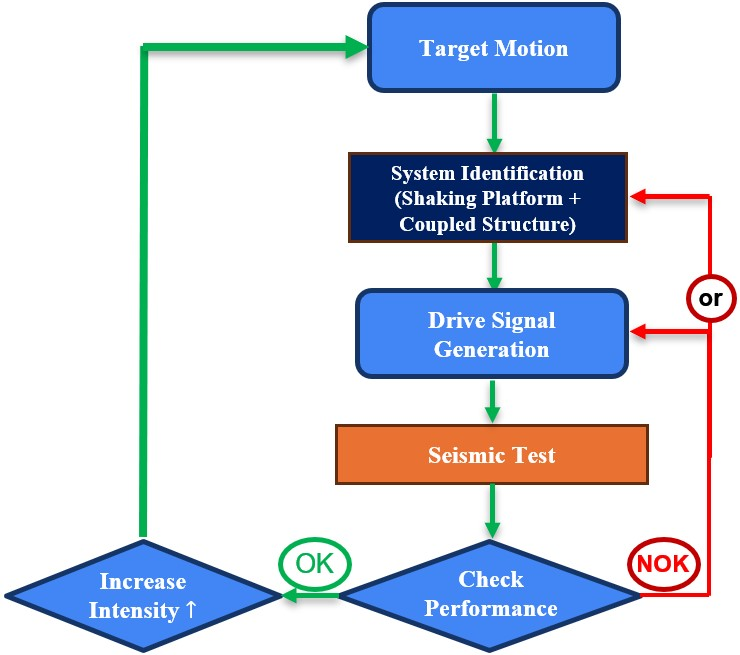
\includegraphics[width=0.51\linewidth]{Intro/lnec_test_process_diagram.jpg}
    \caption{Work flow diagram of the seismic testing process at LNEC. }
    \label{fig_lnec_test_process_diagram}
\end{figure}

Controller settings (proportional and integral gains) are set beforehand. During the test, the structure is subjected to a series of tests steps with different earthquake amplitudes. Initially, the test is carried out with the earthquake at a reduced amplitude, assessing the subsequent damage. The procedure is then repeated with the same earthquake, but at a higher amplitude, again assessing the damage, and so on until a defined amplitude is reached, which usually corresponds to the original amplitude of the earthquake.\par

Before each test, an identification of the system's transfer function is carried out, driving the system with a limited-band pink noise displacement signal (pink noise has a slope of -10dB/decade). %, always with the same amplitude, to determine the system's transfer function.
This transfer function is then used in the drive signal generation algorithm. Throughout this process, the amplitude of the reference signal increases progressively, and it is expected that the structure will enter a non-linear regime, either due to the behaviour of some of its components or the damage accumulated over the test steps carried out. Additional system identifications may be performed—particularly before increasing the target motion intensity—whenever it is verified that the adapted drivers are overcompensating specific frequency bands, a behaviour typically associated with poor identification.

At the end of each test, the system's performance is evaluated by comparing the response spectrum of the reference signal with that of the signal recorded at the platform.\par

However, it is not always possible to achieve satisfactory performance with the command signal synthesized initially, and it may be necessary to generate more than one command signal and carry out additional tests at the same amplitude. This procedure, although necessary in some situations, should be avoided as it induces additional damage to the structure.

In addition, the system faces physical limitations inherent to the equipment, namely with regard to the finite field of displacement, velocity and acceleration, which must be duly considered during the tests.

% \begin{figure}[H]
%     \centering
%         \begin{tikzpicture}[circ/.style = {draw, circle, minimum size=8mm, inner sep=0pt}, thick ]
%         % sum_r2
%         \node[circ]  (sum_r2) at (0,   0) {};
%         \node[left=-1pt] at (sum_r2.center){\small $+$};
%         \node[below=-1pt] at (sum_r2.center){\small $-$};

%         % C
%         \node[draw, fill=SkyBlue!50, minimum width=15mm, minimum height=10mm, right=8mm of sum_r2 ] (C) {$C_{closed}$};

%         % another S0 
%         \node[draw, fill=Green!50,, minimum width=15mm, minimum height=10mm , above=5mm of C ] (C_open) {$C_{open} = \frac{1}{\widehat{G}}$};


%         % sum_r1
%         \node[circ , right=8mm of C ]  (sum_r1) {$+$};

%         % G0
%         \node[draw, fill=Cyan!50, minimum width=15mm, minimum height=10mm , right=6mm of sum_r1 ] (G0)    {$G$};

%         % % sum_v
%         % \node[circ, , right=8mm of G0 ]  (sum_v) {$+$};

%         % H0
%         % \node[draw, fill=Yellow!50, minimum width=15mm, minimum height=10mm, above=8mm of sum_v ] (H0)  {$H_0$};

%         %--- Input r2 ---
%         \draw[-latex] (-2, 0) -- node[above,at start,xshift=2mm]{$r(t)$} (sum_r2);

%         %--- sum_r2 -> C -> sum_r1 ---
%         \draw[-latex] (sum_r2) -- node[above]{$e(t)$} (C);
%         \draw[-latex] (C) -- (sum_r1);

%         %--- r1 drops into sum_r1 from above ---
%         % \draw[-latex] ([yshift=10mm]sum_r1.north) -- (sum_r1);
%         \draw[-latex] (C_open) -- (C_open -| sum_r1) -- (sum_r1.north);

%         % r --> C_open
%         \draw[-latex] ([xshift=-5mm] sum_r2.west) -- ([xshift=-5mm] sum_r2.west |- C_open.west) -- (C_open.west);

%         %--- sum_r1 -> G0 ---
%         \draw[-latex] (sum_r1) -- node[above]{$u(t)$} (G0);

%         % %--- G0 -> sum_v ---
%         \draw[-latex] (G0) -- node[above,at end, xshift=-3mm]{$y(t)$}      ([xshift=12mm] G0.east);
%         %--- e -> H0 -> v -> sum_v ---
%         % \draw[-latex] ([yshift=8mm]H0.north) node[left,yshift=-2mm]{$e(t)$} -- (H0);
%         % \draw[-latex] ([yshift=10mm] sum_v.north) -- node[right]{$v$} (sum_v);S

%         %--- sum_v -> y output ---
%         % \draw[-latex] (sum_v) -- node[above]{$y(t)$} ([xshift=12mm] sum_v.east);

%         %--- Feedback: y branches back to sum_r2 bottom ---
%         \coordinate (ybranch) at ([xshift=5mm] G0.east);
%         \draw (ybranch) --+(0, -1.2) -- (0, -1.2);
%         \draw[-latex] (0, -1.2) -- (sum_r2.south);

%     \end{tikzpicture}
% \caption{LNEC Seismic table offline drive generation and closed-loop control}%, with position $X_{ref}$ as input and force applied to the platen $F_P$ as output.
% \label{tikz_LNEC_control} 
% \end{figure}

\subsection{Response Spectrum}

The response spectrum constitutes a fundamental analytical tool in earthquake engineering and structural dynamics, providing the basis for contemporary seismic design methodologies. It characterises the maximum response (in terms of displacement, velocity, or acceleration) of a structure idealised as a single-degree-of-freedom (1DOF) system when subjected to a ground motion. The procedure by which a response spectrum is determined is illustrated schematically in Figure \ref{fig_response_spectrum_schematic}: the peak response amplitudes {\textcircled{\raisebox{-.9pt}{3}}}, obtained from a suite of 1DOF mass-spring-damper oscillators with 5\% critical damping and varying natural frequencies {\textcircled{\raisebox{-.9pt}{2}}} subjected to a seismic excitation {\textcircled{\raisebox{-.9pt}{1}}}, are plotted as a function of natural frequency {\textcircled{\raisebox{-.9pt}{4}}}.
\begin{figure}[H]
        \centering
    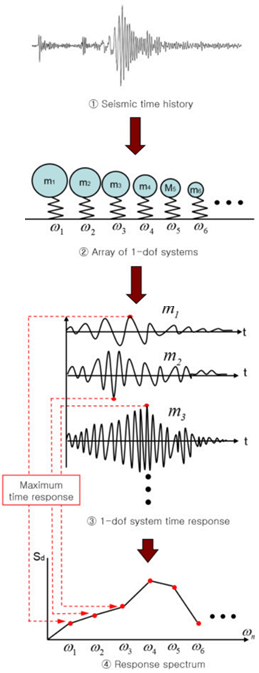
\includegraphics[width=0.42\textwidth]{response_spectrum_schematic.png}
    \caption{ Schematized process of determining a response spectrum }
    \label{fig_response_spectrum_schematic}
\end{figure}

The relevance of this concept to the present work stems from the fact that the performance of the shaking table is assessed primarily on the basis of its capacity to reproduce earthquake ground motion response spectra, evaluated over a frequency range of 0.1 to 30Hz.

The key aspects of the response spectrum are:
\begin{itemize}[noitemsep, topsep=0pt, leftmargin=*]
    \item Ground Motion Dependency: The response spectrum is derived from an earthquake acceleration time history, though displacement and velocity response spectra may also be employed depending on the application. Distinct seismic records yield distinct response spectra; however, the inverse is not necessarily true, as multiple time-domain signals can produce an equivalent response spectrum. This property is particularly relevant in seismic structural design, where building codes require the generation of artificial accelerograms spectrum-compatible with a prescribed target response spectrum.
    \item Structural Dynamic Properties: The spectral response is governed by the dynamic characteristics of the structure, namely its natural frequency and damping ratio. Structures with differing dynamic properties will exhibit distinct response profiles under identical ground motion excitation.
    \item Spectral Quantity: Depending on the nature of the analysis, the response spectrum may be derived from the acceleration, velocity, or displacement time histories. The principal spectral quantities and their respective applications include:
    \begin{itemize}[noitemsep, topsep=0pt, leftmargin=*]
        \item Spectral Acceleration: Employed in force-based design procedures.
        \item Spectral Velocity: Employed in energy-based design.
        \item Spectral Displacement: Employed in displacement-based design.
    \end{itemize}
\end{itemize}

The main applications of the response spectrum in Civil Engineering include:
\begin{itemize}[noitemsep, topsep=0pt, leftmargin=*]
    \item Seismic Design of Buildings and Bridges: Response spectra provide the basis for the determination of equivalent seismic design forces.
    \item Code-Based Seismic Analysis: Established design standards, such as \textit{ASCE 7}, \textit{Eurocode 8}, and \textit{IS 1893}, prescribe standard response spectra and associated design rules for structures located in seismically active regions.
    \item Performance-Based Seismic Design (PBSD): Response spectra are employed to predict and quantify structural behaviour across a range of seismic hazard levels.
    \item Experimental Testing: Response spectra serve a dual role in experimental contexts, both as a metric for evaluating the fidelity of testing equipment, such as shaking tables, in reproducing target ground motions, and as the basis for generating spectrum-compatible artificial accelerograms for use as input excitations.
\end{itemize}

% \begin{figure}[H]
% % \begin{minipage}[t]{0.54\textwidth}%\setlength{\parindent}{15pt}
% %     \vspace{0pt}
% %     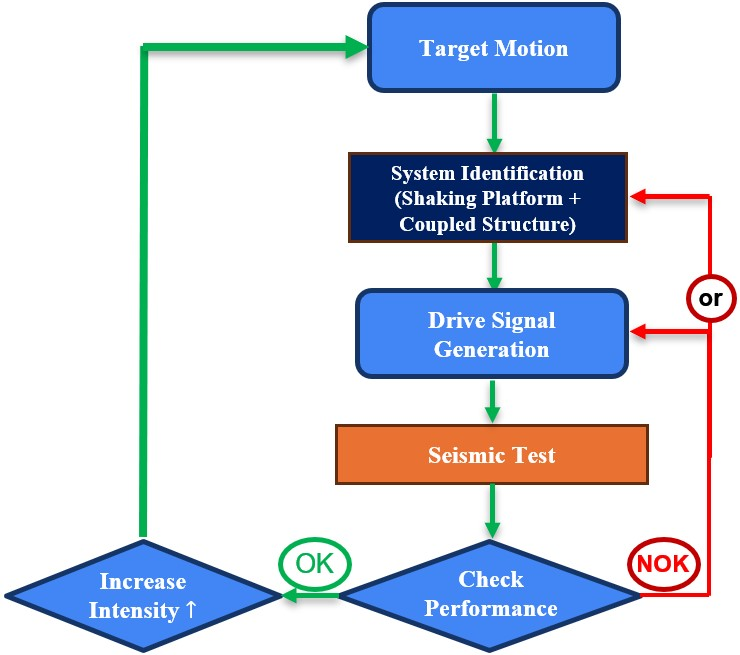
\includegraphics[width=\linewidth]{Intro/lnec_test_process_diagram.jpg}
% %     \caption{Work flow diagram of the seismic testing process at LNEC. }
% %     \label{fig_lnec_test_process_diagram}
% % \end{minipage}
% % \hfill
% % \begin{minipage}[t]{0.40\textwidth}
%     % \vspace{0pt}
%     \centering
%     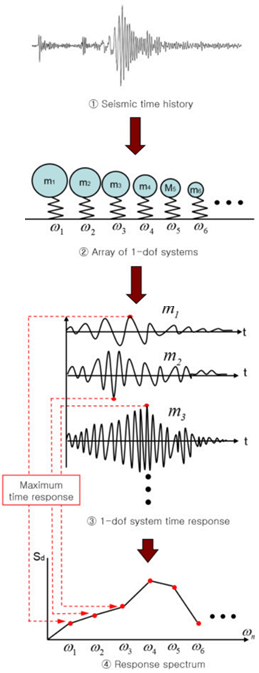
\includegraphics[width=0.45\textwidth]{response_spectrum_schematic.png}
%     \caption{ Schematized process of determining a response spectrum }
%     \label{fig_response_spectrum_schematic}
% % \end{minipage}
% \end{figure}


\pagebreak
\section{Objectives}
The objective of this work is to implement a controller, or strategy, to ensure that the seismic platform reproduces the test seismic signal (reference/earthquake) as accurately as possible, taking into account the following aspects:
\begin{itemize}
    \item The amplitude of the earthquake increases progressively with each test during the experimental campaign;
    \item Before each test, an identification of the system is carried out at a reduced amplitude (to avoid damaging the model). One objective will be to assess the feasibility of using the earthquake response to identify, or complement the identified model, and cover higher amplitudes.
    \item The command signal, generated offline, is imposed on the seismic platform without prior evaluation, by simulation, as to its effectiveness in creating the desired output at the seismic platform;
    \item The seismic platform system with 1 degree of freedom (ST1D) is capable of testing models with a mass of up to 5 tons, and operates in a band of interest from 0 to 25 Hertz. It also has the following limitations (which should be confirmed in laboratory tests):
    \begin{itemize}
        \item Maximum displacement, in absolute value, of 100 mm
            \item Maximum speed, in absolute value, of 0.4 m/s
        \item Maximum acceleration, in absolute value, of 25 m/s$^2$
    \end{itemize}
    \item The model to be tested may initially exhibit linear behaviour, but as it degrades, it inevitably becomes non-linear. In general, the structures tested have two vibration modes in the seismic platform's band of interest, whose initial characteristics (without damage) are:
    \begin{itemize}[label=$\diamond$]
    \item $1.5 \leq f_1 (\mathrm{Hz}) \leq 4$
    \item $2 \leq \xi_1 (\%) \leq 5$
    \item $6 \leq f_2 (\mathrm{Hz}) \leq 10$
    \item $5 \leq \xi_2 (\%) \leq 15$
    
    In damaged structures, damping can reach:
    \begin{itemize}
        \item $\xi_1 = 10\%$
        \item $\xi_2 = 25\%$
    \end{itemize}
    \end{itemize}

    \item Performance will be evaluated by comparing the response spectrum of the measured signal with that of the reference signal.
\end{itemize}

\clearpage
\section{Outline of Dissertation}
%Taking into account the main objectives mentioned above, a comprehensive numerical and experimental study was carried out to identify suitable control strategies capable of improving system performance, evaluated in terms of response spectrum, when compared with the current LNEC control strategy. The work carried out in this study is the embodies the thesis structured into six chapters, including the current one, while the final chapter outlines the main conclusions and directions for future work: 
Taking into account the main objectives delineated above, a comprehensive numerical and experimental investigation was conducted to identify and evaluate control strategies capable of enhancing the dynamic performance of the system, assessed in terms of response spectrum replication accuracy, relative to the control strategy currently employed at LNEC. The body of work arising from this study is structured into six chapters, including the present one, the contents of which are summarised as follows:

\textbf{Chapter 1} introduces the problem, beginning with the experimental activity carried out at LNEC in the field of earthquake engineering. It includes a description of the control strategy currently in use and a brief explanation of the response spectrum concept, employed to evaluate system performance. The chapter concludes by outlining the main objectives of the thesis and its overall structure.

\textbf{Chapter 2} presents a literature review on experimental testing in earthquake engineering, highlighting the main experimental methods and their purpose. Control strategies available for use with LNEC's shaking table are also reviewed, and the chapter closes with recent developments in shaking table control.

\textbf{Chapter 3} introduces the essential concepts in control theory and closed-loop system identification. It further provides a detailed description of the identification and control strategies applied in this work, supported by application examples.

\textbf{Chapter 4} presents a model for LNEC's uniaxial shaking table, which is subsequently used to evaluate, in a simulation environment, the performance of three control strategies: LNEC's iterative method, a tuned PID-F controller, and an optimal controller.

\textbf{Chapter 5} applies the proposed closed-loop identification method to LNEC's uniaxial electrodynamic shaker. The identified model is then used to evaluate the performance of the proposed control strategies, which are compared with LNEC's iterative method.

\textbf{Chapter 6} concludes the thesis with the main findings of this work, discussing the advantages of the proposed methods over the strategy currently employed at LNEC, and identifying directions for future work.

\clearpage

\chapter[Literature Review on Experimental Testing in Earthquake Engineering]{Literature Review on Experimental\\Testing in Earthquake Engineering}
 %\chapter{Revisão do Estado da Arte}\label{sec:sota}
%Realizar uma pesquisa abrangente sobre técnicas para ensaios sísmicos, com foco em ensaios em plataforma sísmica. Incluir uma análise dos métodos de ensaio, configurações de montagem, bem como da instrumentação utilizada para medição e controlo dos equipamentos.

\section{The Purpose of Experimental Testing} %Simulation and Reality: 
% IS SEISMIC EXPERIMENTAL TESTING OF STRCUTURES STILL NECESSARY, DESPITE THE EVOLUTION OF COMPUTACIONAL SIMULATIONS?
% https://consensus.app/search/is-seismic-experimental-testing-of-strcutures-stil/L-Ya5EyiQSqxujE68BaTQw/?utm_source=share&utm_medium=clipboard
\hspace{\parindent}While computational simulations have become highly sophisticated and efficient, they still face limitations in accurately modelling complex, nonlinear, or poorly understood behaviours, especially in components with significant uncertainties or novel materials. 
Studies show that numerical simulations, even with advanced methods, require experimental benchmarks to ensure accuracy, especially for complex interactions. Machine learning approaches also rely on experimental data for training and updating models. Experimental testing provides critical validation and calibration for these models.

In summary, seismic experimental testing remains indispensable for validating models, understanding complex behaviours, and ensuring structural safety. The trend is toward integrated approaches using both experimental and computational tools to achieve the most reliable seismic performance assessments.\citep{williams2001, Zhang2023Experimentally, Liu2020Experimental, Bahraq2021Numerical, Malomo2022M-DEM, Qiu2024Seismic, Yavas2023A, Mokhtari2023A}

\section{An Overview of Experimental Methods}
% IN THE FIELD OF earthquake engineering, WHAT ARE THE MOST WIDELY USED EXPERIMENTAL METHODS?
% https://consensus.app/search/in-the-field-of-seismic-engineering-what-are-the-m/QdpmhhJsS76N_XJJZcAGgA/
According to \cite{williams2001}, the most widely used experimental methods in the field of earthquake engineering are:
\begin{itemize}
    \item \textbf{Shaking Table Tests:} Shaking tables simulate real earthquake ground motions on structural or soil models, allowing direct observation of dynamic response and failure mechanisms. They are considered the gold standard for dynamic testing of buildings, bridges, tunnels, and other infrastructures. 
    They are used for both full-scale and scaled models, including innovative in-situ testing with mobile shaking tables \citep{williams2001,Bousias2017Experimental,Abovyan2024Method,Tsinidis2020Seismic,DeFelice2016Methods,El-Emam2018Experimental}. 
    \item \textbf{Pseudo-Dynamic Testing} and \textbf{Hybrid Simulation:} In pseudo-dynamic testing, loads are applied over a greatly expanded timescale with the dynamic behaviour of the structure accounted for computationally, from the measured reaction forces and the calculated inertia, damping and loading force. In hybrid simulation, just like pseudo-dynamic testing, a combination of physical testing and numerical modelling is used, but the experimental part of the process is performed at higher rates (than pseudo-dynamic testing) to have time to perform the numerical simulations and execute the time step on the experiment, allowing the test specimen to be 'almost' under the dynamic regime (would be the full dynamic regime for a unitary time scale). These methods are widely used for complex or large structures where full dynamic testing is impractical \citep{williams2001,Bousias2017Experimental}.
    \item \textbf{Static and Cyclic Loading Tests:} These tests apply static or cyclic loads to materials, structural elements, or systems to evaluate their properties for specific studies, such as earthquake engineering. Testing protocols using static and/or cyclic loads are common standard protocols considered to determine component's properties such as concrete anchors, piers or beam to column assemblies \citep{williams2001,Bousias2017Experimental,Fiorino2016Experimental}.
    \item \textbf{Centrifuge Modelling:} Centrifuge tests use scaled soil-structure models spun at high speeds to replicate in situ stress conditions (i.e. gravitational stresses), enabling realistic simulation of soil-structure interaction during earthquakes, especially for underground structures such as tunnels. This method is mostly focused on testing geotechnical models, not structures, to evaluate their stress-strain behaviour and failure mechanisms, namely the strength, stiffness and capacity of foundations for bridges and buildings, settlement of embankments, stability of slopes, earth retaining structures tunnel stability and seawalls. \citep{williams2001,Tsinidis2020Seismic}.
    \item \textbf{Surface Based Seismic Methods:} This method is used for site characterization, through passive-source (microtremor) and active-source techniques, to determine ground shear-wave velocity profiles \citep{Luke2008Characterizing}.
    \item \textbf{Laboratory Fault Slip Experiments:} This method is used to study fault mechanics and induced seismicity, employing shear-flow, triaxial, and injection-driven tests \citep{Ji2022Laboratory,Dong2022Investigations}.
    \item \textbf{Vibration Machines:} The testing equipment is installed on site, and employed for simulating seismic impacts on buildings and models, offering a cost-effective alternative for certain applications \citep{Abovyan2024Method}.
    \item \textbf{Explosive Charges:} Arrays of explosive charges are used to simulate earthquake ground motions at large scale (very uncommon method) \citep{williams2001}.
\end{itemize}

Real-time hybrid simulation (RTHS) and substructural shake table testing are of special interest since they allow for the evaluation of large and/or complex structures by combining physical and numerical models of substructures, which enhances testing flexibility, enabling improved studies of high-frequency and/or nonlinear behaviours, while also reducing experimental costs. Real-time hybrid simulation method is illustrated in figure \ref{fig_hybrid} for 3 different configurations \citep{Tang2020Performance}. In \cite{Lin2024Implementation} a different configuration is implemented, resorting to onboard actuators, as shown in figure \ref{fig_onboard_actuators}, in order to circumvent the additional stroke length, velocity, and acceleration requirements for ground-based actuators, and the control challenges they pose.

\begin{figure}
    \centering
    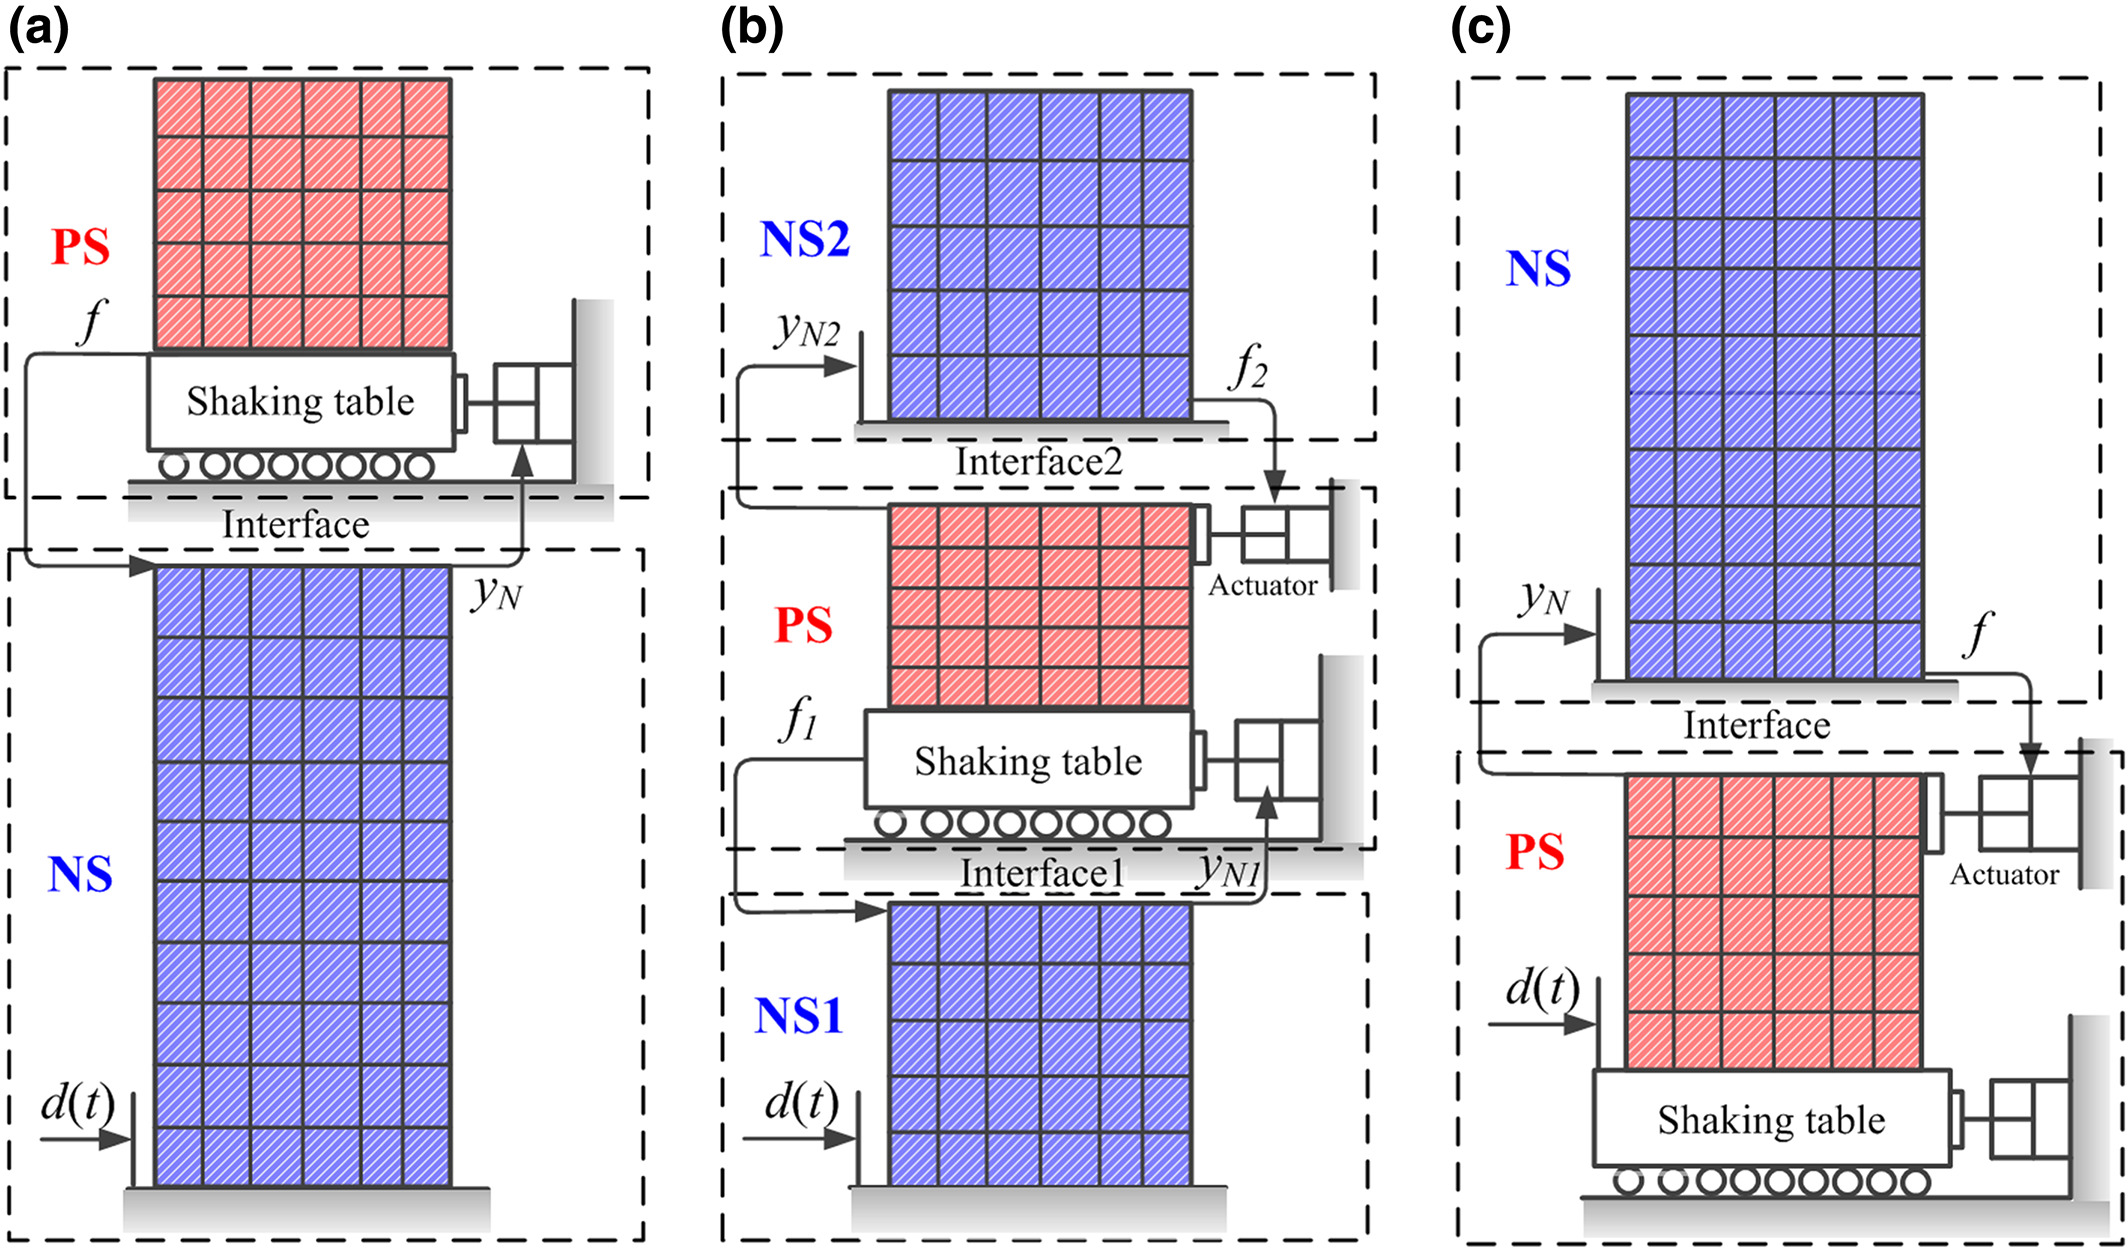
\includegraphics[width=\linewidth]{Lit_Review/stc2611-fig-0001-m.jpg}
    \caption{Shaking table-based real-time dynamic hybrid testing systems: (a) upper, (b) middle and (c) lower portion tested physically. Abbreviations: NS, numerical substructure; PS, physical substructure \citep{Tang2020Performance}}
    \label{fig_hybrid}
\end{figure}

\begin{figure}
    \centering
    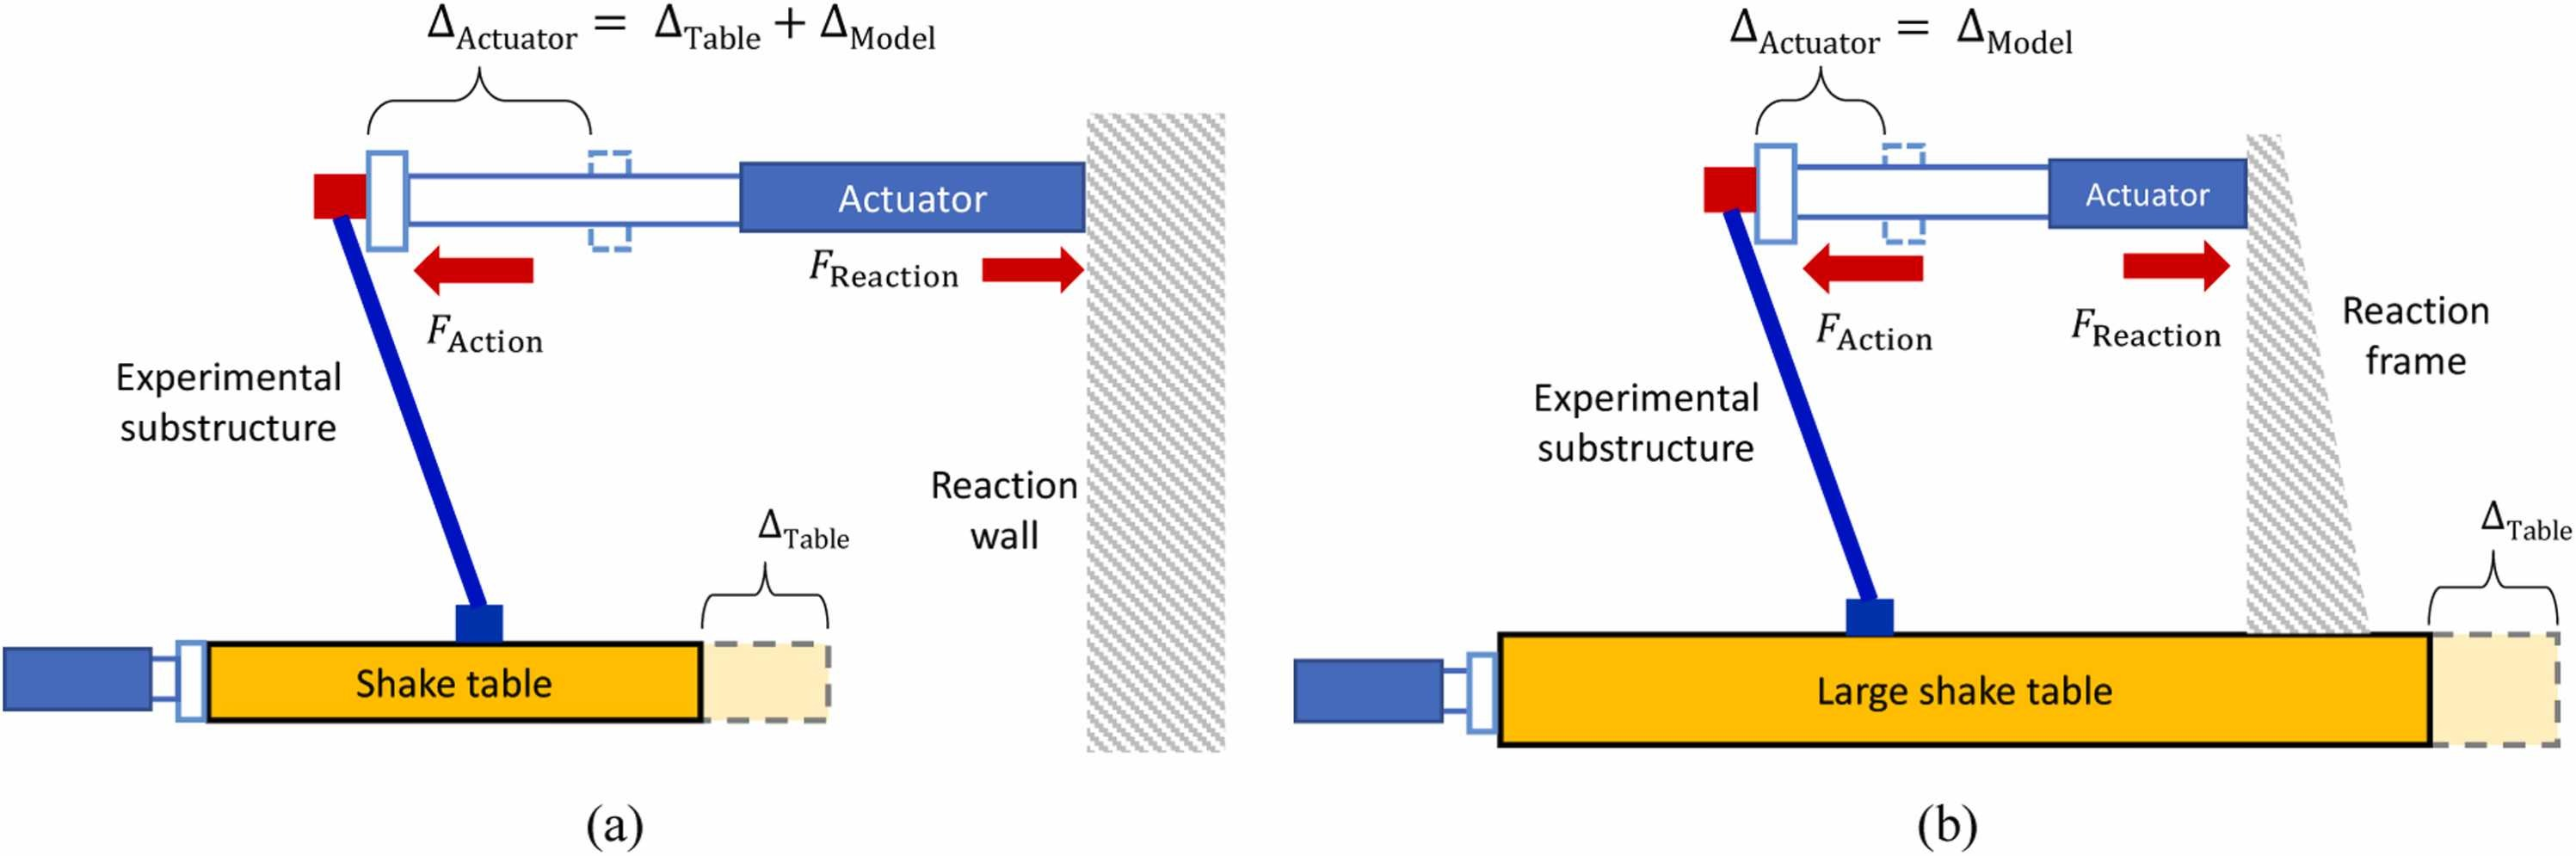
\includegraphics[width=\linewidth]{Lit_Review/onboard_actuators.jpg}
    \caption{Shake table RTHS with (a) ground-based actuators and (b) onboard actuators. \citep{Lin2024Implementation}}
    \label{fig_onboard_actuators}
\end{figure}

\section{Shaking Table Control Strategies}

Shaking-table control strategies typically begin with the offline generation of a drive signal using the inverse model of the system and the desired reference motion. This drive signal is then applied to the system, which usually incorporates a linear controller, most commonly a Proportional-Integral-Derivative (PID) controller, using actuator feedback signals (displacement, velocity, or acceleration) \citep{williams2001}, and that is the basis of the OLI control strategy. Indeed, PID controllers remain widely used in most test systems, including shaking-table and hybrid testing platforms \citep{tekeste2021}. However, alternative control approaches have been proposed in the literature, including: Acceleration Trajectory Tracking Control (ATTC) \citep{nakata2010}; Displacement feedforward-feedback controller using an optimal controller \citep{phillips2012}; Model-based feedforward-feedback controller for acceleration tracking \citep{phillips2014}; Minimal control synthesis (MCS) strategy, which is feedback-feedforward adaptive control strategy including the inverse model in line with the reference signal \citep{stoten2001}.

% SEISMIC TABLE CONTROL FOR DYNAMIC TESTING OF STRUCTURES & CAN ADAPTIVE CONTROL IMPROVE SHAKING TABLE TEST ACCURACY?
% https://consensus.app/search/adaptive-control-shaking-tables/P-JOknr3Slax_foG1eKOKg/?utm_source=share&utm_medium=clipboard

Recent works developed in this field show that advanced control methods such as active disturbance rejection control (ADRC) with adaptive model-based state estimators (AMSE) and extended state observer (ESO), as applied in \cite{Lei2023Disturbance} and illustrated in figure \ref{fig_ADRC-AMSE}, and also nonlinear signal-based control \citep{Enokida2019Nonlinear}, have significantly improved the accuracy and stability of shaking table operations, especially for reproducing complex seismic waveforms and handling nonlinear structural responses. In \cite{Tian2021Offline}, the use of offline iterative control combined with frequency-splitting techniques enabled double-layer shaking tables to achieve both high payload capacity and a wide frequency bandwidth. This advancement allows for the effective testing of high-rigidity structures — such as dams and nuclear power plant facilities - which are characterised by high fundamental frequencies.  Meanwhile, in the development of a budget-focused testing facility, \cite{Parajuli2024Development} adopted a brushed DC motor as the shaking table actuator and applied a proportional-derivative (PD) controller to achieve motion control, offering a cost-effective alternative to more complex systems.

\begin{figure}
    \centering
    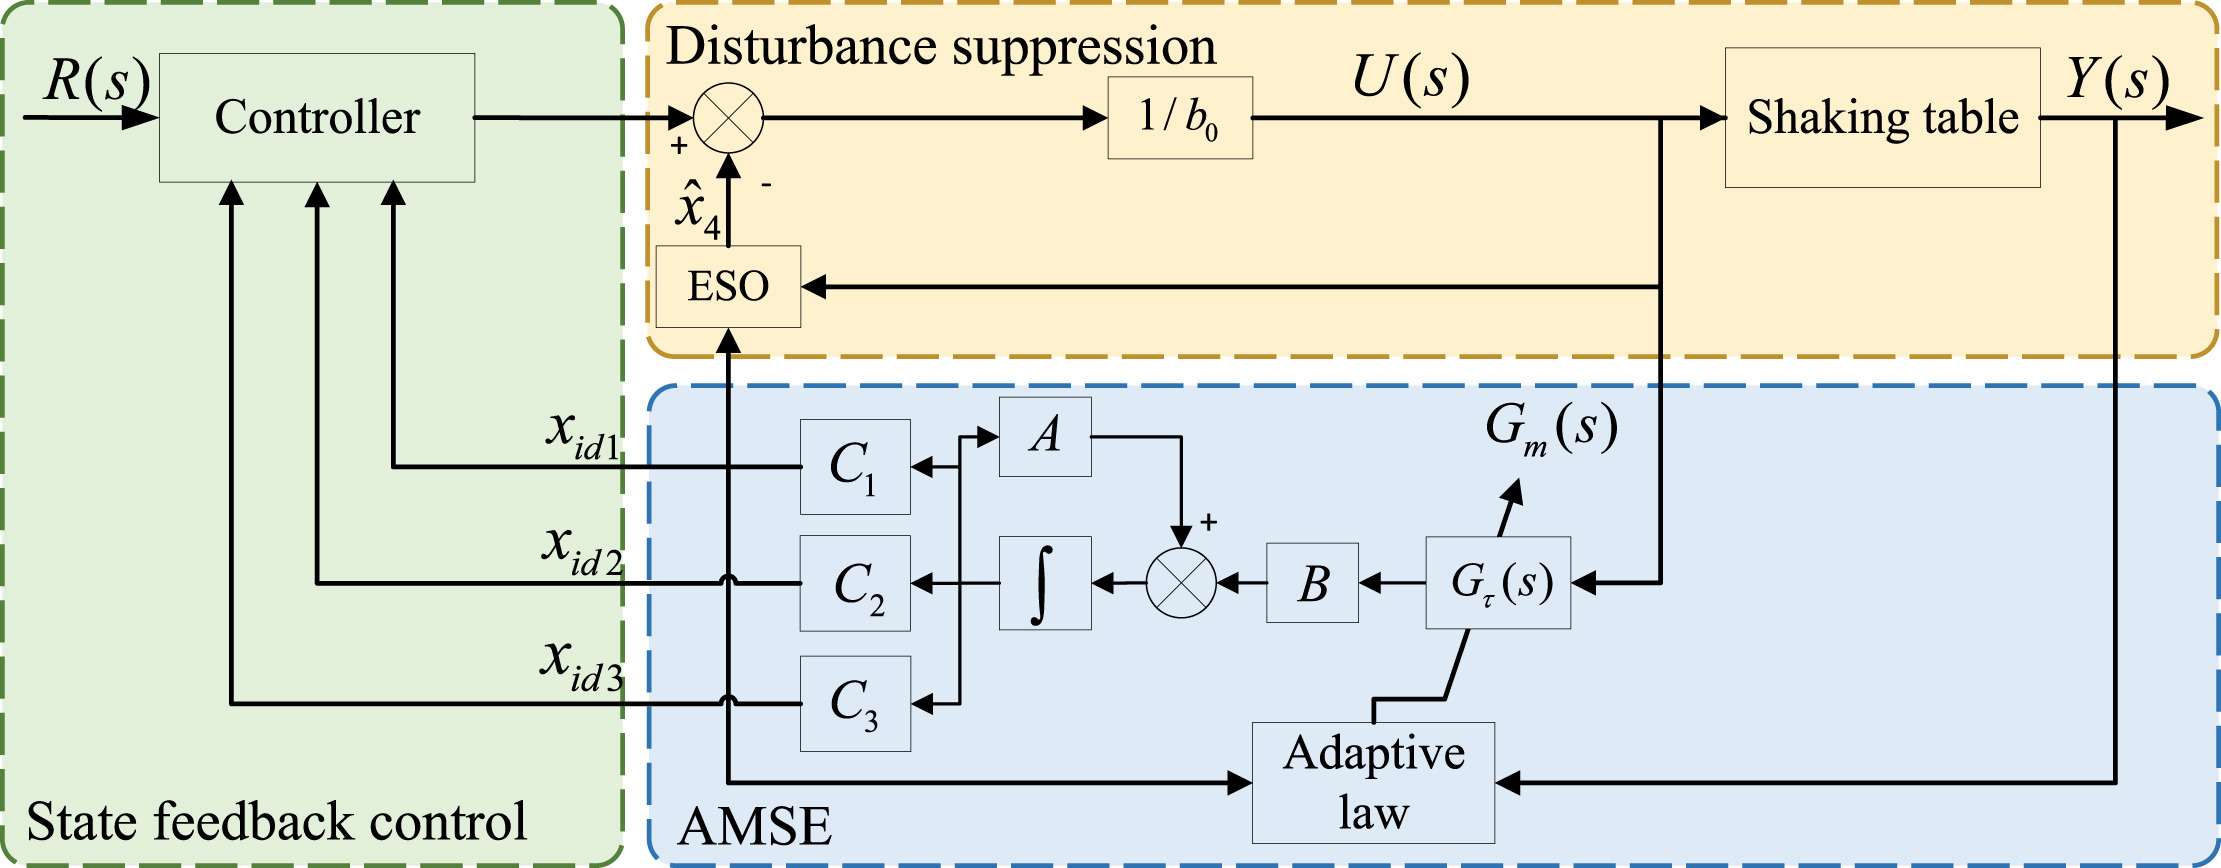
\includegraphics[width=0.7\linewidth]{Lit_Review/ADRC_AMSE.jpg}
    \caption{Structure diagram of AMSE-ADRC \citep{Lei2023Disturbance}}
    \label{fig_ADRC-AMSE}
\end{figure}

% Can adaptive control improve shaking table test accuracy?

% Adaptive control has been shown to significantly improve the accuracy of shaking table tests for dynamic structural evaluation:
% \begin{itemize}
%     \item %Enhanced Tracking and Stability: 
%     Adaptive control methods, such as adaptive-model-based state estimators, model reference adaptive control, and adaptive sliding mode control, have been shown to improve both the stability and tracking accuracy of shaking tables, especially under varying test conditions and for systems with nonlinear dynamics %1456891415+2 MORE.
%     \item %Compensation for Uncertainties: 
%     Adaptive controllers can dynamically adjust to compensate for amplitude and phase deviations, system nonlinearities, and parameter uncertainties, leading to more precise seismic waveform reproduction and better handling of control-structure interaction effects %161418.
%     \item %Superior Performance over Conventional Methods: 
%     Comparative studies demonstrate that adaptive control strategies outperform traditional fixed-parameter controllers (such as PID or three-variable controllers) in both time and frequency domains, providing better acceleration tracking and robustness to specimen uncertainties %4561314.
%     \item %Practical Validation: 
%     Experimental and simulation results across multiple studies confirm that adaptive control approaches—such as online adaptive compensation, adaptive inverse control, and functional link adaptive controllers—consistently yield higher fidelity in replicating target motions and structural responses during shaking table tests %15789101113+5 MORE.
% \end{itemize}

%% Only the most important papers
%H ybrid and adaptive control for waveform replication
Among the most impactful publications on shaking table control, \cite{Gang2013Adaptive} proposed a hybrid controller combining offline feed-forward inverse modelling with online adaptive inverse control (AIC) to improve acceleration waveform replication in electro-hydraulic shaking tables, extending the frequency bandwidth and achieving higher fidelity than conventional approaches. %2
Another paper by the same authors builds on this work by introducing a delay compensator, an internal model controller, and an offline inverse model compensator (OIMC), resulting in improved tracking accuracy compared with three-variable and adaptive controllers alone \citep{Shen2017Acceleration}. The corresponding control system block diagrams are shown in figure \ref{fig_shen2017_control}. %1

In \cite{Yachun2018A}, a two-loop controller combining model reference adaptive control with three-variable control adapts drive signals to different payloads, improving tracking performance in both the time and frequency domains compared with standard three-variable control. %3

In parallel, other techniques have been proposed to mitigate the influence of external disturbances, as in the work of  \cite{Seki2009Adaptive}, where an adaptive notch-filter-based feedback compensator is used to identify and suppress frequency-varying reaction forces generated by rotating machinery, thereby improving motion accuracy. %6

In \cite{Zhang2016Robust}, an adaptive sliding mode controller with a reaching law was developed for a double shaking table system, achieving fast response, high precision, and robust tracking and synchronization under uncertainties and disturbances. %4

In \cite{Ryu2017Real-time}, a nonlinear tracking controller based on feedback linearization combined with an extended Kalman filter enabled real-time control of shaking tables subjected to nonlinear hysteretic structural behaviour, maintaining motion fidelity at specific structural locations. %5

\begin{figure}%[H]
\begin{subfigure}{0.48\textwidth}
    \centering
    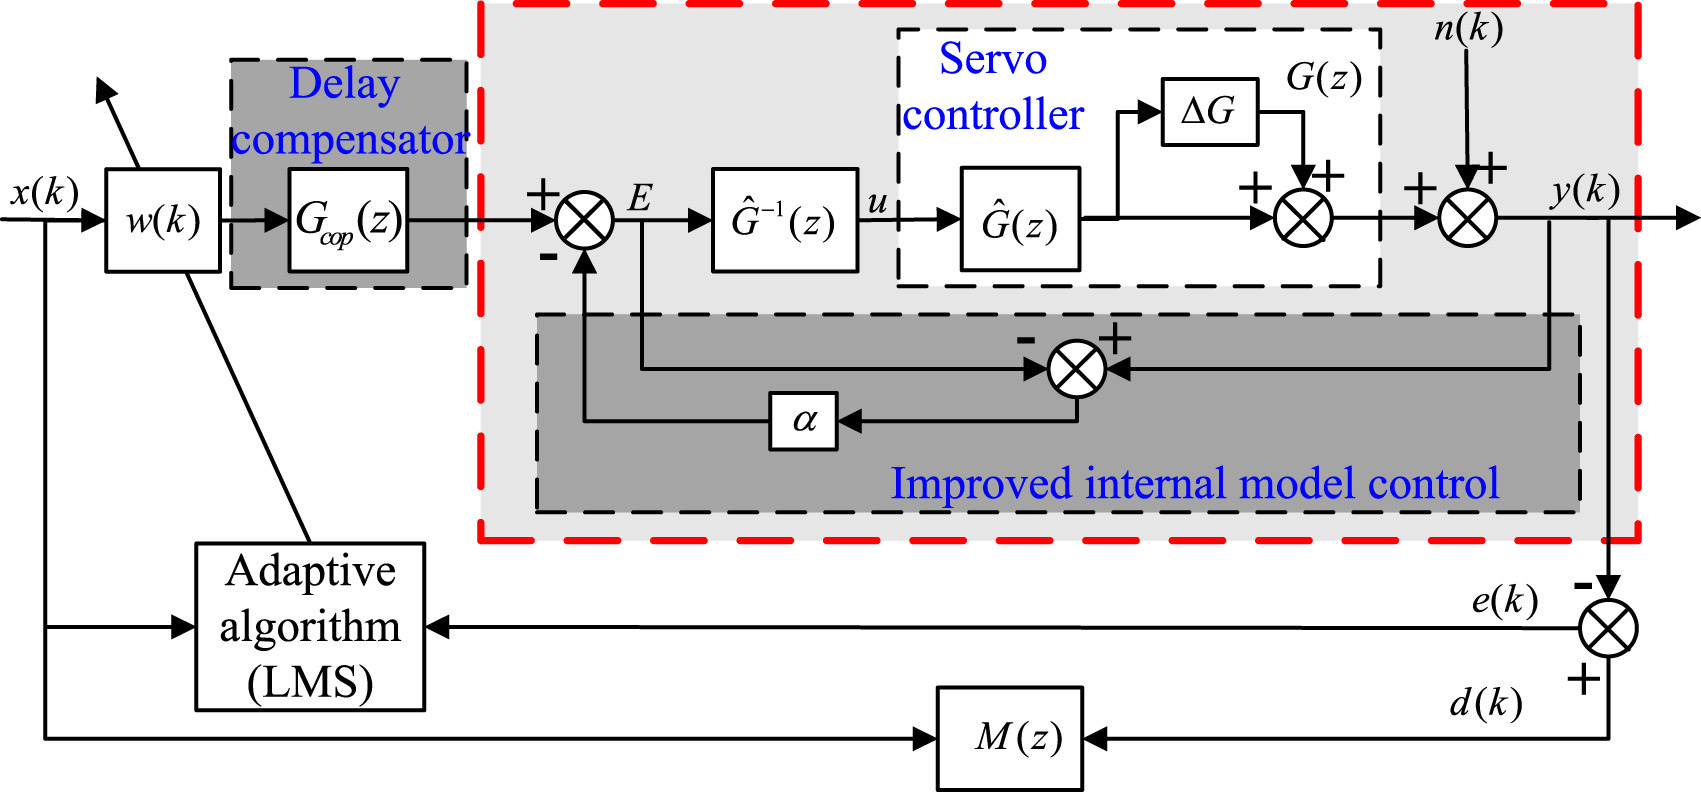
\includegraphics[width=\textwidth]{Lit_Review/1-s2.0-S0019057817305037-gr6_lrg.jpg}
    \caption{Complete control system}
\end{subfigure}
\hfill
\begin{subfigure}{0.49\textwidth}
    \centering
    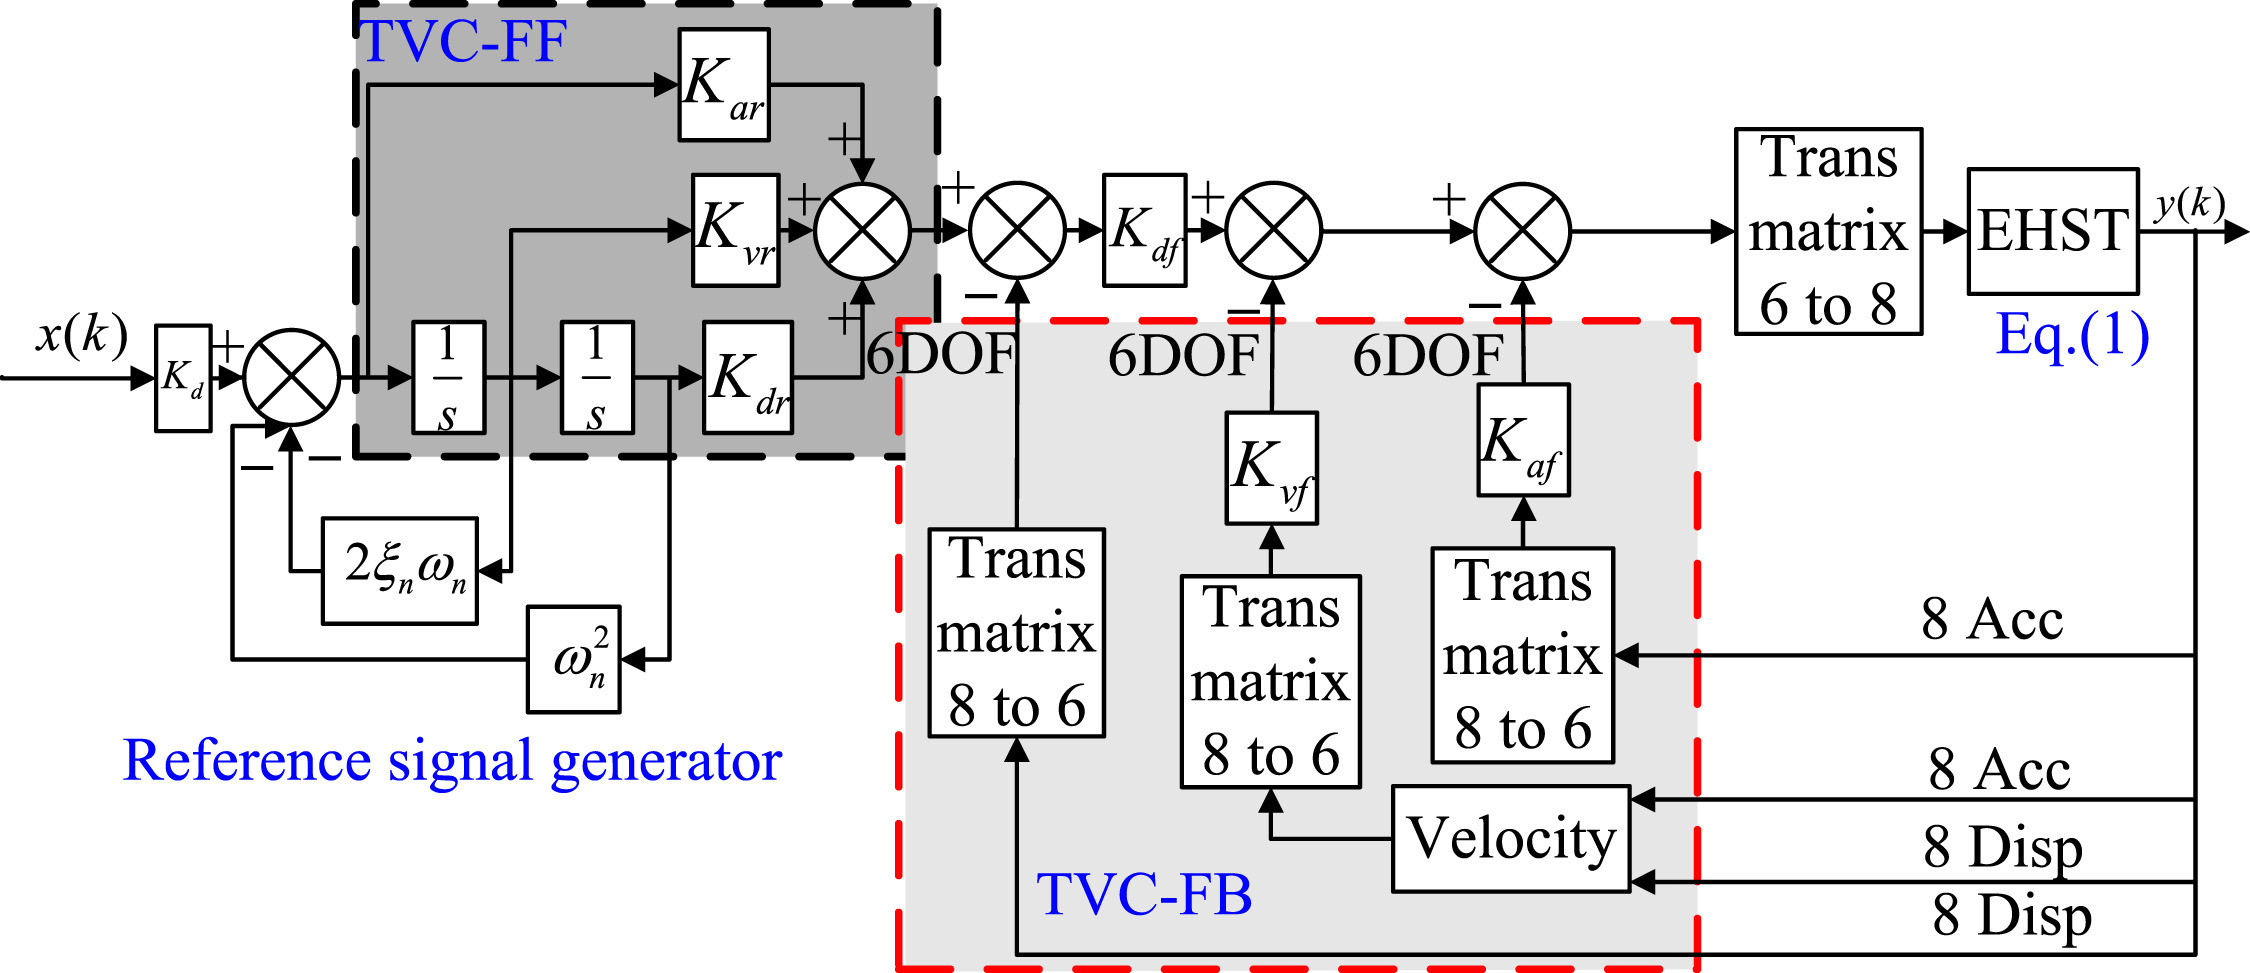
\includegraphics[width=\textwidth]{Lit_Review/1-s2.0-S0019057817305037-gr5_lrg.jpg}
    \caption{Servo controller}
\end{subfigure}
\caption{Control system block diagram in \cite{Shen2017Acceleration}}
\label{fig_shen2017_control}
\end{figure}


In summary, the recent developments on shaking tables control strategies are toward hybrid control (offline + online), with robust, and adaptive, and nonlinear model-based methods to keep shaking tables accurate during the test, where the test specimens often exhibit evolving and nonlinear dynamics.

\subsection{LNEC's Shaking Tables Control Strategies}

The hydraulic and control system original supplier for LNEC's shaking tables, MTS Systems Corporation, provided several control strategies tailored to different testing conditions, each presenting distinct advantages and drawbacks:

\begin{itemize}
    \item Three-Variable Control (TVC), whose block diagram is depicted in figure \ref{fig_TVC}, also known in control theory literature as state variable control \citep{ogata2010}, which combines the displacement, velocity and acceleration feedback \citep{williams2001}. In this implementation only one state variable is the primary control variable, with the others serving only as compensation signals to improve damping and stability;
    \item Adaptive Harmonic Cancellation (AHC), whose block diagram is depicted in figure \ref{fig_AHC}, is suitable for sinusoidal signals (fixed frequency or sweep). This method greatly reduces harmonic distortion of the response of a control system driven by a sinusoidal command. It measures the harmonic distortion directly and adapts in real time the cancelling waveform applied directly to the control system input; 
    \item Adaptive Inverse Control (AIC), whose block diagram is depicted in Figure \ref{fig_AIC}, was presented in \cite{widrow2007} as a control strategy suitable for non-sinusoidal signals in linear systems. This method consists of a control compensation technique that augments a fixed-gain controller to correct closed-loop gain and phase irregularities, thereby improving control fidelity. In addition, in multichannel control systems with cross-coupled dynamics, it significantly reduces cross-coupling disturbances between control channels. The method measures the control system dynamics directly and modifies the control compensation accordingly in real time, making it possible to adapt to changing system dynamics; 
    \item Amplitude/Phase Control (APC), whose block diagram is depicted in figure \ref{fig_APC}, is suitable for sinusoidal signals (fixed frequency and sweep) and predominantly linear systems, and often used in conjunction with AHC to reduce distortions in nonlinear systems. This is a control compensation technique that augments a fixed-gain controller to correct for closed-loop amplitude and phase irregularities in order to improve control fidelity. It measures control system dynamics directly and modifies the control compensation accordingly in real time, making it possible to adapt to changing system dynamics; 
    \item Online Iteration (OLI), whose block diagram is depicted in figure \ref{fig_OLI}, is suitable for nonlinear systems and non-sinusoidal waveforms. This is a control technique that repeatedly modifies the command input to a control system on an individual sample-by-sample basis until the control system response is almost a perfect replica of the original desired command. This last strategy was deemed the most appropriate and versatile for earthquake engineering applications, as structures may exhibit nonlinear behaviour or sustain damage during testing, and is the control method currently implemented at LNEC's ST3D.
\end{itemize}

\begin{figure}%[H]
    \centering
    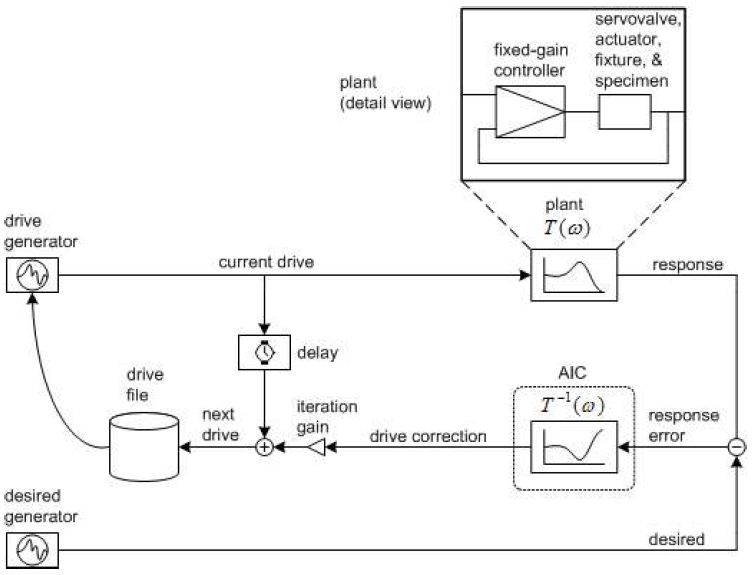
\includegraphics[width=0.9\textwidth]{MTSsystems/OLI.png}
    \caption{Online Iteration (OLI)}
    \label{fig_OLI}
\end{figure}

\chapter{ System Identification \& Control}

This chapter presents the theoretical foundations underlying the system identification and control strategies employed in this work. It is organized into three main parts. The first part, Section 3.1, establishes the signal and system analysis framework, covering the definitions, notation, and properties of signals processed by discrete linear time-invariant (LTI) systems. The second part, Section 3.2, addresses control system design, progressing from open-loop to closed-loop architectures, and introducing the specific controllers considered in this work: a PID-F controller, and full state feedback control with optimal control formulation, including the concepts of controllability, observability, and state estimation. The third part, Section 3.3, tackles the problem of system identification in closed-loop settings, discussing the limitations of classical spectral analysis methods and presenting the Two-Stage Method as a suitable approach for closed-loop identification.

\section{Signals \& System Analysis}
\subsection{General Definitions \& Notation}
For a signal discretized with sampling time $T_s$:
\begin{itemize}
    \item The delay operator $z^{-1}$ corresponds to a delay of one sampling time;
    \item The forward operator $z$ corresponds to a forward time shift of one sampling time;
    \item A delay/forward shift of $k$ sampling times $T_s$ corresponds to $z^{-k}$ or $z^k$, respectively;
    \item $G(z)$, in upper case, designates a transfer function, while the lower case $g(k)$ is the corresponding pulse response computed at time instant $t = k T_s$, and both are related by:
        \begin{equation}
            G(z) = \sum_{k=-\infty}^{\infty} g(k)\, z^{-k}
        \end{equation}
    \item The complex-valued function $G(e^{i\omega})$ is the evaluation of the transfer function $G(z)$ on the unit circle $z=e^{i\omega}$ in the complex plain, and is referred to as the frequency response of a discrete time system. This differs from continuos time systems where a frequency response $G(i\omega)$ of a given continuous transfer function $G(s)$ is given by its evaluation on the imaginary axis $s = i\omega$;
    \item Various equations will have the notation eased by omitting the function variables to improve readability;
    \item The circumflex denotes an estimated model or property from some data (ex. $\widehat{G}(z)$).
\end{itemize}


\subsection{Properties of stationary stochastic signals processed by discrete LTI systems}

The autocorrelation of signal $x(t)$, and the cross correlation between signals $x(t)$ and $y(t)$, for a time delay $\tau$ is given, respectively, by:
\begin{align}
    R_{x}(\tau)  =& \, E\left[ \, x(t)\, x(t-\tau) \, \right] \\[2mm]
    R_{yx}(\tau) =& \, E\left[ \, y(t)\, x(t-\tau) \, \right] 
\end{align} 

And the power spectral density of signal $x(t)$:
\begin{equation}
    \Phi_{x}(\omega)  = \sum_{\tau= -\infty}^{\infty} R_{x}(\tau) e^{-i \omega \tau}
\end{equation}

And the power cross-spectral density of signals $x(t)$ and $y(t)$:
\begin{equation}
    \Phi_{yx}(\omega) = \sum_{\tau= -\infty}^{\infty} R_{yx}(\tau)e^{-i \omega \tau} 
\end{equation} 

For an LTI system as in figure \ref{tikz_LTI_sys}, where $y(t) = G(z) \cdot x(t)$, with $x$ and $y$ quasi-stationary signals, we have the following properties:
\begin{align}
    R_{yx}(\tau) =& \, G(z) \,  R_{x}(\tau)  \\
                    =& \, g(\tau) \star  R_{x}(\tau) \nonumber \\[2mm]
    R_{xy}(\tau) =& \, G^{*}(z) \,  R_{x}(\tau)   \\
                    =& \, g(-\tau) \star  R_{x}(\tau) \nonumber \\[2mm]
    R_{yy}(\tau) =& \, G^{*}(z) \, G(z) \, R_{x}(\tau)   \\
                    =& \, g(-\tau) \star g(\tau) \star R_{x}(\tau) \\[2mm]
    \Phi_{yx}(\omega) =& \, G(e^{i\omega}) \,  \Phi_{x}(\omega) \\[2mm]
    \Phi_{xy}(\omega) =& \, G^{*}(e^{i\omega}) \,  \Phi_{x}(\omega) \\[2mm]
    \Phi_{y}(\omega)  =& \, G(e^{i\omega}) \, G^{*}(e^{i\omega}) \,\Phi_{x}(\omega)\\
                        =& \, \left|G(e^{i\omega})\right|^2 \Phi_{x}(\omega) \nonumber 
\end{align}

The way in which LTI systems process correlation is also illustrated in figure \ref{tikz_correlation}:
\begin{figure}[H]
\begin{minipage}{0.47\textwidth}
    \centering
    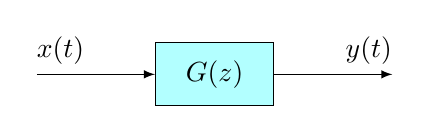
\begin{tikzpicture}
        \node[draw, fill=Cyan!30, minimum width=15mm, minimum height=8mm  ] (G) at (0,0)   {$G(z)$};
        % \node[draw, fill=Cyan!30, minimum width=15mm, minimum height=8mm , below= 4mm of G ] (G_2)  {$G_{2}(z)$};

        \draw[-latex] ([xshift=-15mm]G.west) -- node[above,at start, xshift=3mm]{$x(t)$} (G); % x
        \draw[-latex] (G) -- node[above,at end, xshift=-3mm]{$y(t)$} ([xshift=15mm] G.east); % y

        % \draw [-latex] ([xshift=-7mm]G.west) -- ([xshift=-7mm]G_2.west) -- (G_2.west); %branch
        % \draw[-latex] (G_2) -- node[above,at end, xshift=-2mm]{$w$} ([xshift=15mm] G_2.east); %w
    \end{tikzpicture}
    \caption{LTI system}\label{tikz_LTI_sys} 
\end{minipage}
\hfill
\begin{minipage}{0.51\textwidth}
    \centering
    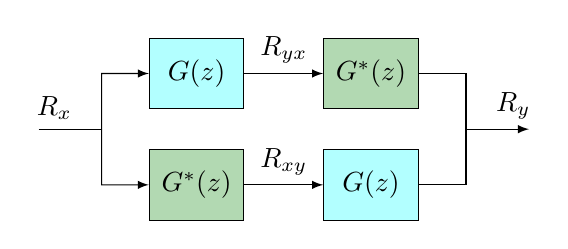
\begin{tikzpicture}
        \node[draw, fill=Cyan!30, minimum width=12mm, minimum height=9mm  ] (G) at (0,0)   {$G(z)$};
        \node[draw, fill=Green!30, minimum width=12mm, minimum height=9mm, right= 10mm  of G] (G*)  {$G^{*}(z)$};
        \draw[-latex] (G.east) -- node[above]{$R_{yx}$} (G*.west);
        % \draw[-latex] (G*.east) -- node[above,at end, xshift=-2mm]{$R_y$} ([xshift=10mm] G*.east);

        \node[draw, fill=Green!30, minimum width=12mm, minimum height=9mm, below= 5mm  of G] (G*_bottom)  {$G^{*}(z)$};
        \node[draw, fill=Cyan!30, minimum width=12mm, minimum height=9mm, below= 5mm  of G*] (G_bottom)  {$G(z)$};
        \draw[-latex] (G*_bottom.east) -- node[above]{$R_{xy}$} (G_bottom.west);
        % \draw[-latex] (G_bottom.east) -- node[above,at end, xshift=-2mm]{$R_y$} ([xshift=10mm] G_bottom.east);

        \coordinate (branch) at ($([xshift=-6mm] G.west)!0.5!([xshift=-6mm] G*_bottom.west)$); % input: branch point centered vertically between G and Gs_bottom
        \draw([xshift=-8mm] branch) -- node[above, at start, xshift=2mm]{$R_x$} (branch);
        \draw[-latex] (branch) -- ([xshift=-6mm] G.west)         -- (G.west);
        \draw[-latex] (branch) -- ([xshift=-6mm] G*_bottom.west) -- (G*_bottom.west);

        \coordinate (branch_right) at ($([xshift=6mm] G*.east)!0.5!([xshift=6mm] G_bottom.east)$);
        \draw[-latex](branch_right) -- node[ above, at end, xshift=-2mm]{$R_y$} ([xshift=8mm]branch_right);
        \draw  (G*.east)       -- ([xshift=6mm]G*.east)       -- (branch_right) ;
        \draw  (G_bottom.east) -- ([xshift=6mm]G_bottom.east) -- (branch_right) ;
    \end{tikzpicture}
    \caption{Illustration of how linear systems transform correlation signals}\label{tikz_correlation} %correlation signals, which is also entirely analogous to the way they transform spectral density signals. 
\end{minipage}
\end{figure}


In the case of two systems which generate an output from a common input signal, as in figure \ref{tikz_two_sys_common_input}, then $y_2$ can be given as function of $y_1$, and we have the following relations:
    \begin{align}
        y_{2}(t) =& \, G_{2}(z)\, x(t) = G_{2}(z)\, G_{1}^{-1}(z) \, y_{1}(t) \\[3mm]
        \Phi_{y_ {2}y_{1}}(\omega) =& G_{2} G_{1}^{-1} \, \Phi_{y_{1}}(\omega)  =  G_{2}(e^{i\omega}) G_{1}^{*}(e^{i\omega}) \, \Phi_{x}(\omega)
    \end{align}

\begin{figure}[H]
\centering
    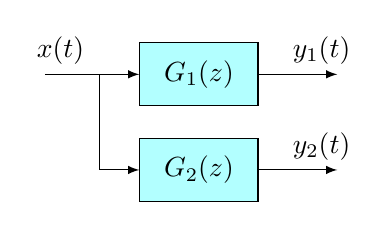
\begin{tikzpicture}
        \node[draw, fill=Cyan!30, minimum width=15mm, minimum height=8mm  ] (G) at (0,0)   {$G_{1}(z)$};
        \node[draw, fill=Cyan!30, minimum width=15mm, minimum height=8mm , below= 4mm of G ] (G_2)  {$G_{2}(z)$};

        \draw[-latex] ([xshift=-12mm]G.west) -- node[above,at start, xshift=2mm]{$x(t)$} (G); % x
        \draw[-latex] (G) -- node[above,at end, xshift=-2mm]{$y_1(t)$} ([xshift=10mm] G.east); % y_1

        \draw [-latex] ([xshift=-5mm]G.west) -- ([xshift=-5mm]G_2.west) -- (G_2.west); %branch
        \draw[-latex] (G_2) -- node[above,at end, xshift=-2mm]{$y_2(t)$} ([xshift=10mm] G_2.east); %y_2
    \end{tikzpicture}\vspace{-2mm}
    \caption{Two systems with a common input signal}\label{tikz_two_sys_common_input} 
\end{figure}

%\clearpage


% \begin{figure}[H]
%     \centering
%     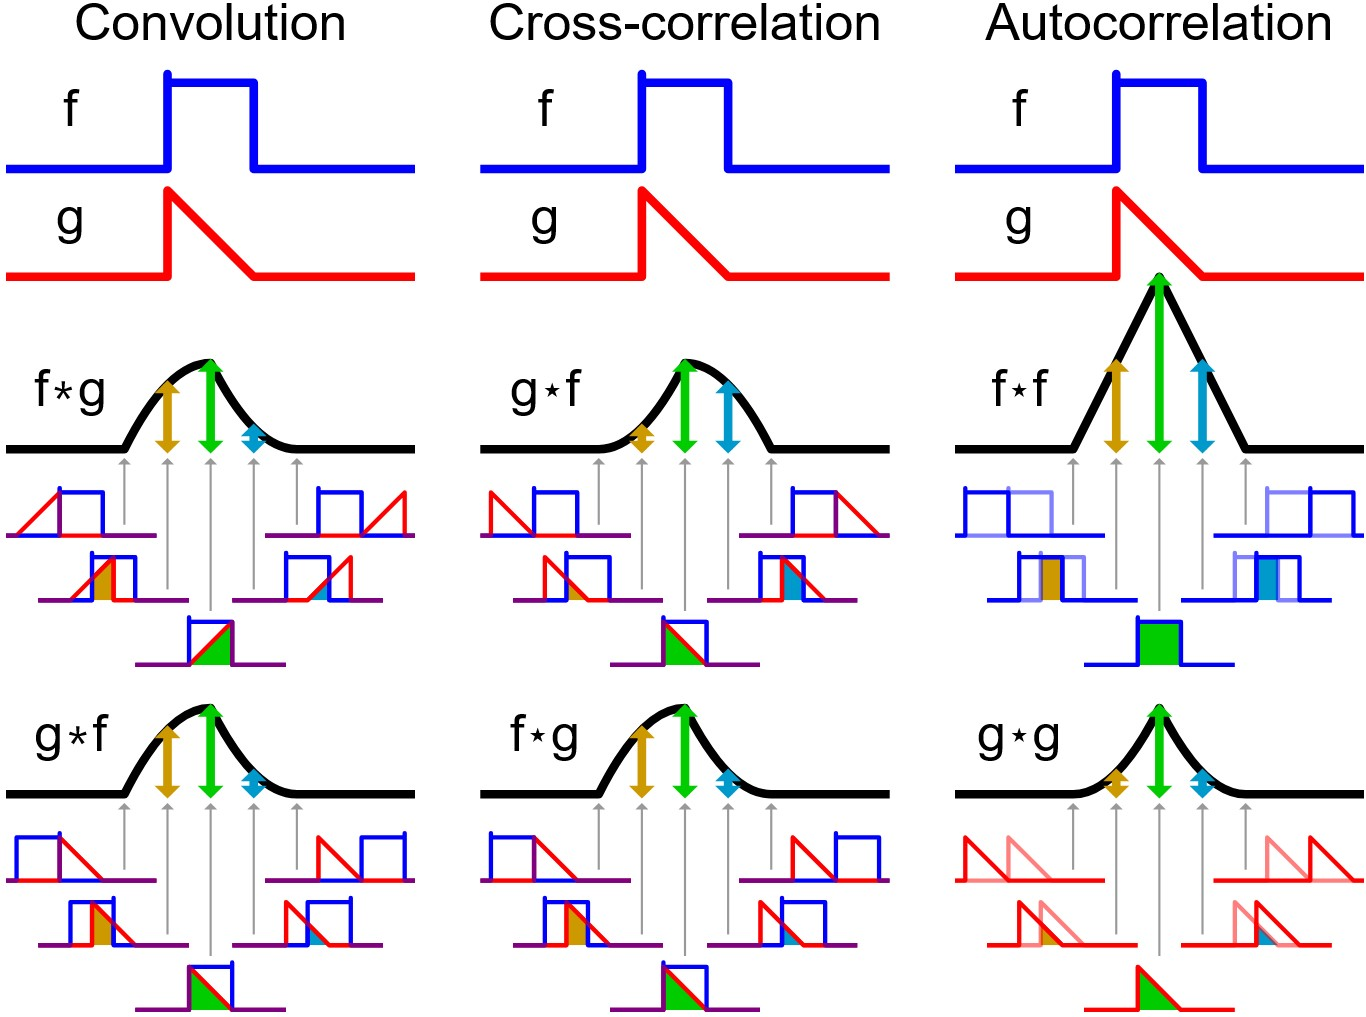
\includegraphics[width=0.8\linewidth]{convolution_correlations.jpg}
%     \caption{Visualization of convolution, cross-correlation, and autocorrelation. The output of the computation is represented by the shaded area, and is shown for 5 different lag values. (Adapted from original of \cite{cmglee_convolution_correlation})}% For the operations involving function f, and assuming the height of f is 1.0, the value of the result at 5 different points is indicated by the shaded area below each point. Note that placing $f \star g$ next to $R_{gf}$, instead of next to $R_{fg}$ facilitates comparing the 5 snapshots below the graphs. They are identical sets, except for the orientation of function f, as denoted by the little bump on its left-hand corner. But since f is symmetric, the orientation does not matter, which explains why $R_{gf}$ and $f \star g$ are identical in this example
%     \label{convolution_correlations}    
% \end{figure}


\section{Control Systems}

There are two generic configurations for control systems: open-loop control (figure \ref{tikz_Control_Systems_open_loop}) and closed-loop control (figure \ref{tikz_Control_Systems_closed_loop}).
\begin{figure}[H]
    \centering
\begin{minipage}{0.47\textwidth}
    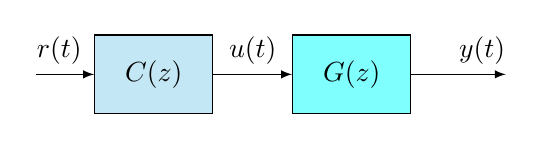
\begin{tikzpicture}
    \node[draw, fill=SkyBlue!50, minimum width=15mm, minimum height=10mm              ] at (0,0) (C) {$C(z)$}; % , label=below:{ Open-loop Controller}
    \node[draw, fill=Cyan!50, minimum width=15mm, minimum height=10mm, right=10mm of C ] (G0)    {$G(z)$};      % , label=below:{System to control}    
    \draw[-latex] (-15mm, 0) -- node[above,at start, xshift=3mm]{$r(t)$} (C);                    % node[below]{reference}     
    \draw[-latex] (C) -- node[above]{$u(t)$}       (G0);                   % node[below]{control action}
    \draw[-latex] (G0) -- node[above,at end, xshift=-3mm]{$y(t)$}      ([xshift=12mm] G0.east);% node[below]{output}        

    \end{tikzpicture}\vspace{-2mm} 
    \caption{Control in open-loop}\label{tikz_Control_Systems_open_loop} 
\end{minipage}
\hfill
\begin{minipage}{0.51\textwidth}
    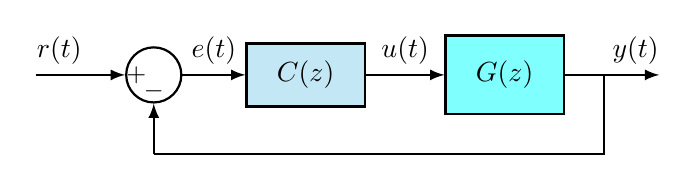
\begin{tikzpicture}[circ/.style = {draw, circle, minimum size=7mm, inner sep=0pt}, thick ]
    % sum_r2
    \node[circ]  (sum_r2) at (0,   0) {};
    \node[left=-1pt] at (sum_r2.center){\small $+$};
    \node[below=-1pt] at (sum_r2.center){\small $-$};

    \node[draw, fill=SkyBlue!50, minimum width=15mm, minimum height=8mm, right=8mm of sum_r2] (C) {$C(z)$};% , label=above:{\parbox{17mm}{\centering closed-loop controller}}
    \node[draw, fill=Cyan!50, minimum width=15mm, minimum height=10mm , right=10mm of C       ] (G0){$G(z)$};% , label=above:{\parbox{15mm}{\centering system to control}}     

    %--- Input r2 ---
    \draw[-latex] (-15mm, 0) -- node[above,at start, xshift=3mm]{$r(t)$}(sum_r2); %node[below]{reference} 
    \draw[-latex] (sum_r2) --  node[above]{$e(t)$}  (C); % node[above]{\parbox{12mm}{\centering tracking error}}
    \draw[-latex] (C) --       node[above]{$u(t)$} (G0); % node[above]{\parbox{12mm}{\centering control action}}
    \draw[-latex] (G0) --      node[above,at end, xshift=-3mm]{$y(t)$} ([xshift=12mm] G0.east); % node[above]{output}                                  

    %--- Feedback: y branches back to sum_r2 bottom ---
    \coordinate (ybranch) at ([xshift=5mm] G0.east);
    \draw (ybranch) --+(0, -1) -- (0, -1);
    \draw[-latex] (0, -1) -- (sum_r2.south);

    \end{tikzpicture}
\caption{Control in closed-loop}%, with position $X_{ref}$ as input and force applied to the platen $F_P$ as output.
\label{tikz_Control_Systems_closed_loop} 
\end{minipage}
\end{figure}

Every control system is a variation and/or a combination of these two configurations. Both add, to the system we want to control, another system called controller which outputs a control action $u(t)$, which is the controlled system's input intended to make the controlled system's output $y(t)$ follow some specified reference $r(t)$ (which is just the desired output).  In a perfectly controlled system the output will match the reference, $y(t) = r(t)$. 

This section aims to give the reader an overview of the essential control configurations, their advantages and limitations, as well as controller structures and design methods. Open-loop and closed-loop architectures are addressed, with the latter including classical output feedback control with a PID-F, and then full state feedback with optimal control and the underlying concepts of controllability, observability, and state estimation. This segment is specially influenced by the work in \cite{DuarteValerio} and \cite{Botto}.

\subsection{Open-Loop Control}
In open-loop control the controller receives the reference that the system should follow and computes a control action.  It is not checked whether the system's output then follows the reference, and the control action is not modified to account for any deviations that occur.

For an open-loop control system we have the following equation:
\begin{equation}
    y(s) = G(s) \, u(s) = G(s)C(s) \, r(s) 
\end{equation}

The main advantages of open-loop control are:
\begin{itemize}
    \item It is conceptually simpler than closed-loop control
    \item It does not require real-time measurement of the output and consequently no sensor for the output variable is required to implement it
    \item If the reference is known in advance, the control action can be computed a priori
\end{itemize}  

Open-loop control works well if two conditions are simultaneously met: A perfect model of the plant exists and there are no unknown disturbances of either the control action or the output. In practice, open-loop control does not work well due to imperfect modelling of the plant, and the existence of process and measurement disturbances, and, more fundamentally, even with a perfect model, open-loop control cannot handle non-minimum phase plants, since inverting their dynamics would require an unstable controller.

\subsubsection{Design of Open-Loop Controllers}

Since we want the output to match the reference:
\begin{equation}
    r(s) = y(s) = G(s)C(s) \, r(s) \Longrightarrow C(s) = \frac{1}{G(s)}
\end{equation}  
The controller should be an inverse model of the system to control. This is problematic if the model of the system is proper, because then the controller is not proper, resulting that additional poles must be added to make the controller proper. These additional poles should be of very high frequency as to preserve the dynamics of the idealised controller (which is just the inverse of the plant) such that it cancels out the dynamics of the plant, and the output matches the reference.

In figure \ref{fig_open}, an example of the reference tracking resulting from open loop control, as in figure \ref{tikz_Control_Systems_open_loop}, with $C = \frac{10 s}{s+1}$, for three cases is shown: 
\begin{itemize}
    \item A perfect identification of the plant: $G_0 = \frac{s+1}{s (s+10)}$, for which the controller was designed (denoted as "nominal" in the legend), highlighting its effectiveness when the plant model is perfect;
    \item A plant with a modelling error: $G_{err} = 1.1 \cdot G_0$, highlighting how this control strategy cannot account for a modelling error of the plant;
    \item The perfect plant with an additive disturbance in the output: $v(t) = sin(2\pi \, t)$ (as in figure \ref{tikz_general_open_loop_sys}), highlighting how this control strategy cannot account for disturbances in the system;
\end{itemize}

\begin{figure}[H]
    \centering
    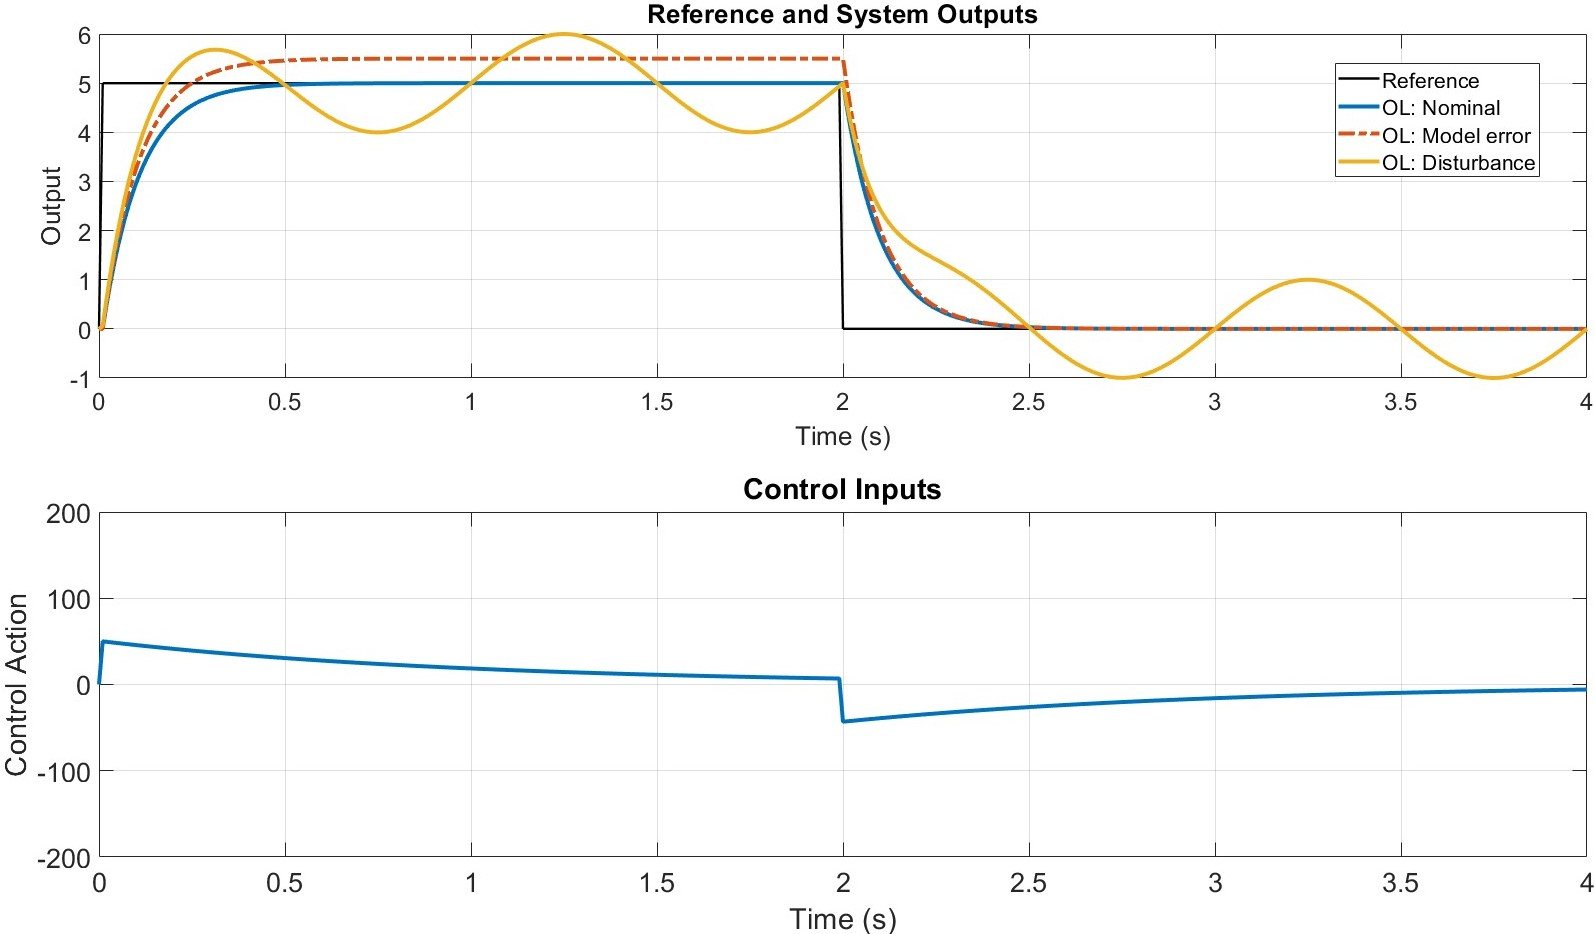
\includegraphics[width=\linewidth]{fig_control_configs/open.jpg}
    \caption{Open-loop control example: Reference \& Outputs}
    \label{fig_open}
\end{figure}

\subsection{Closed-Loop Control}
Closed-loop control uses feedback, meaning the output is being measured and compared with the reference. The difference between the reference and the measured output is the tracking error $e(t)$. In closed-loop control, the tracking error is the input to the controller:
\begin{equation}
    y(s)  = G(s) \, u(s)  = G(s) C(s) e(s)  = G(s) C(s) [r(s) - y(s)]
\end{equation}

The simplest form of closed-loop control is with a proportional controller, $C(s) = K$, meaning the control action is proportional to the tracking error:
\begin{equation}
    u(s)  = C(s)\, e(s) = K \, e(s) \quad, K \in \mathbb{R}
\end{equation}

Thanks to output feedback, closed-loop control can mitigate the effects of disturbances and imperfect models, since the control action is computed from the tracking error, and thus compensates for any deviations from the reference. 

Closed-loop control can also be used to stabilise unstable plants, and the opposite is also true: Badly designed closed-loop control can destabilise stable plants.

In figure \ref{fig_closed}, an example of the reference tracking  resulting from closed loop control, as in figure \ref{tikz_Control_Systems_closed_loop}, with $C = 10 + \frac{50}{s} +  \frac{50 s}{s+1} $, for three cases is shown: 
\begin{itemize}
    \item A perfect identification of the plant: $G_0 = \frac{s+1}{s (s+10)}$ (denoted as "nominal" in the legend);
    \item A plant with a modelling error: $G_{err} = 1.1 \cdot G_0$,  highlighting how this control strategy can compensate for modelling errors of the plant;
    \item The perfect plant with an additive disturbance in the output: $v(t) = sin(2\pi \,t)$ (as in figure \ref{tikz_general_CL_sys}), ,  highlighting how this control strategy can compensate for disturbances in the system;
\end{itemize}

\begin{figure}[H]
    \centering
    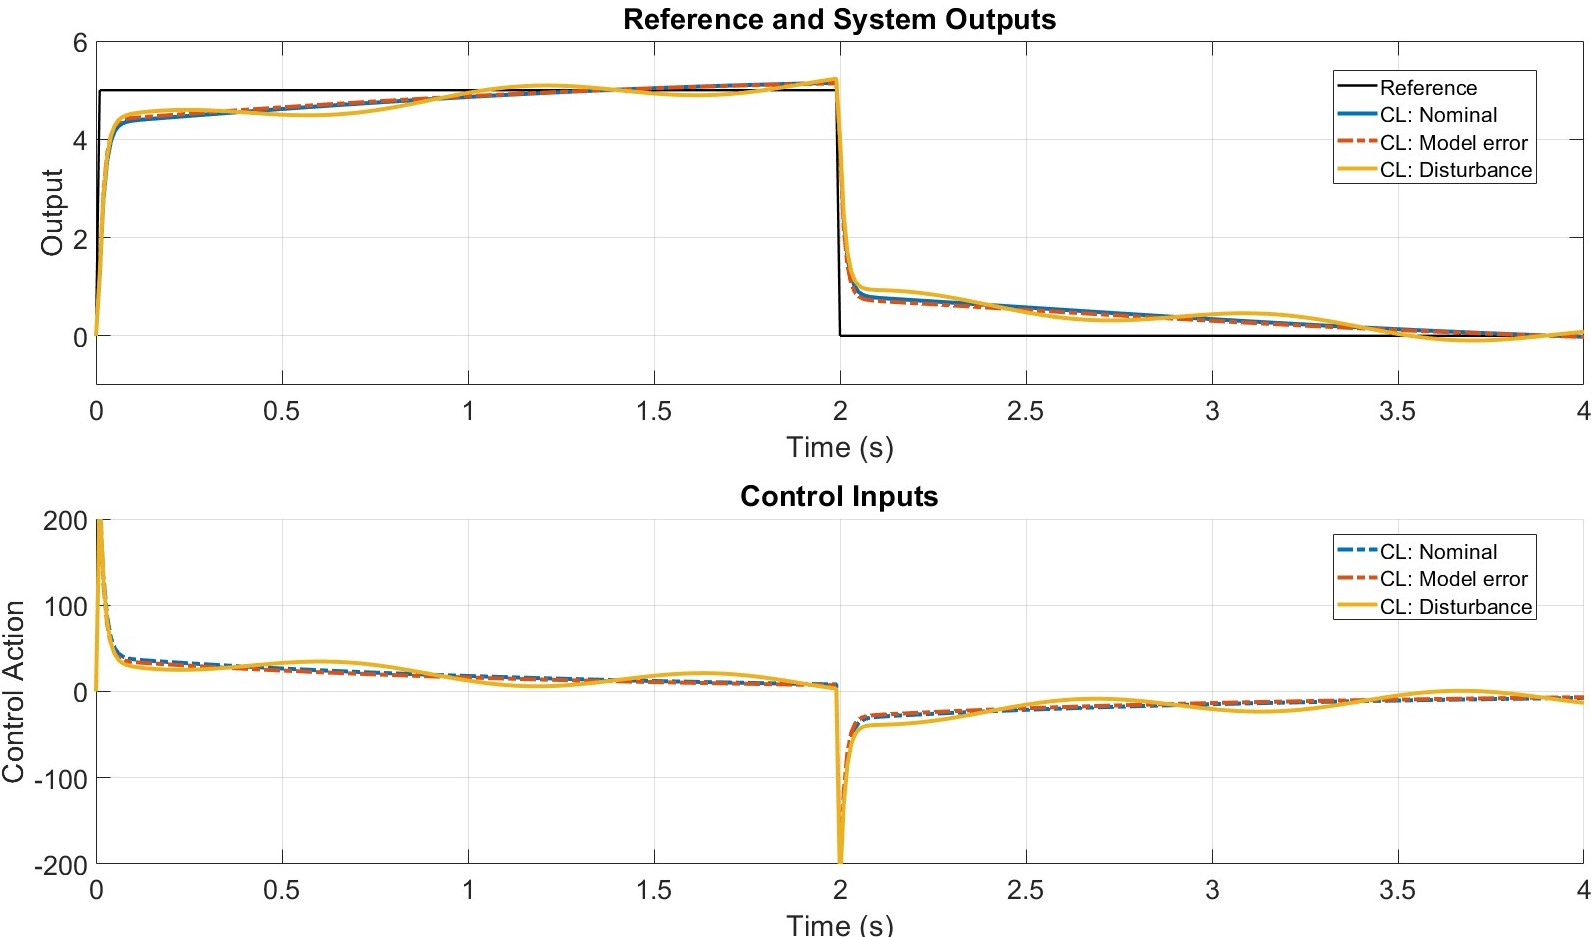
\includegraphics[width=1\linewidth]{fig_control_configs/closed.jpg}
    \caption{Close-loop control example: Reference \& Output} \label{fig_closed}    
\end{figure}

% \begin{figure}[H]
\subsubsection{Combined Open- and Closed-Loop Control}
% \noindent
% \begin{minipage}{0.4\textwidth}\setlength{\parindent}{15pt}
It is possible to combine open-loop and closed-loop control in a single control system. Figure \ref{tikz_Control_Systems_Combined_control} shows this configuration:
    
% \end{minipage}
% \hfill
% \begin{minipage}{0.58\textwidth}
\begin{figure}[H]
    \centering
        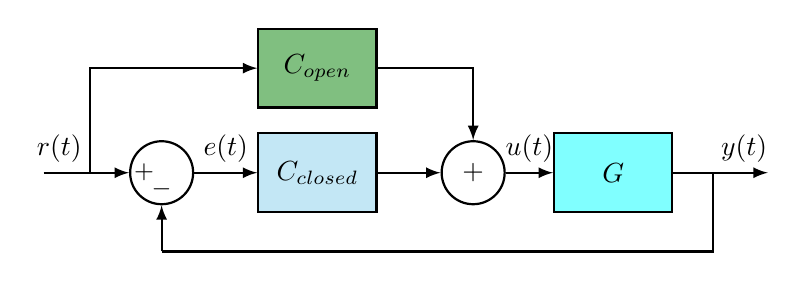
\begin{tikzpicture}[circ/.style = {draw, circle, minimum size=8mm, inner sep=0pt}, thick ]
        % sum_r2
        \node[circ]  (sum_r2) at (0,   0) {};
        \node[left=-1pt] at (sum_r2.center){\small $+$};
        \node[below=-1pt] at (sum_r2.center){\small $-$};

        % C
        \node[draw, fill=SkyBlue!50, minimum width=15mm, minimum height=10mm, right=8mm of sum_r2 ] (C) {$C_{closed}$};

        % another S0 
        \node[draw, fill=Green!50,, minimum width=15mm, minimum height=10mm , above=3mm of C ] (C_open) {$C_{open}$}; % = \frac{1}{\widehat{G}}


        % sum_r1
        \node[circ , right=8mm of C ]  (sum_r1) {$+$};

        % G0
        \node[draw, fill=Cyan!50, minimum width=15mm, minimum height=10mm , right=6mm of sum_r1 ] (G0)    {$G$};

        % % sum_v
        % \node[circ, , right=8mm of G0 ]  (sum_v) {$+$};

        % H0
        % \node[draw, fill=Yellow!50, minimum width=15mm, minimum height=10mm, above=8mm of sum_v ] (H0)  {$H_0$};

        %--- Input r2 ---
        \draw[-latex] (-1.5, 0) -- node[above,at start,xshift=2mm]{$r(t)$} (sum_r2);

        %--- sum_r2 -> C -> sum_r1 ---
        \draw[-latex] (sum_r2) -- node[above]{$e(t)$} (C);
        \draw[-latex] (C) -- (sum_r1);

        %--- r1 drops into sum_r1 from above ---
        % \draw[-latex] ([yshift=10mm]sum_r1.north) -- (sum_r1);
        \draw[-latex] (C_open) -- (C_open -| sum_r1) -- (sum_r1.north);

        % r --> C_open
        \draw[-latex] ([xshift=-5mm] sum_r2.west) -- ([xshift=-5mm] sum_r2.west |- C_open.west) -- (C_open.west);

        %--- sum_r1 -> G0 ---
        \draw[-latex] (sum_r1) -- node[above]{$u(t)$} (G0);

        % %--- G0 -> sum_v ---
        \draw[-latex] (G0) -- node[above,at end, xshift=-3mm]{$y(t)$}      ([xshift=12mm] G0.east);
        %--- e -> H0 -> v -> sum_v ---
        % \draw[-latex] ([yshift=8mm]H0.north) node[left,yshift=-2mm]{$e(t)$} -- (H0);
        % \draw[-latex] ([yshift=10mm] sum_v.north) -- node[right]{$v$} (sum_v);

        %--- sum_v -> y output ---
        % \draw[-latex] (sum_v) -- node[above]{$y(t)$} ([xshift=12mm] sum_v.east);

        %--- Feedback: y branches back to sum_r2 bottom ---
        \coordinate (ybranch) at ([xshift=5mm] G0.east);
        \draw (ybranch) --+(0, -1) -- (0, -1);
        \draw[-latex] (0, -1) -- (sum_r2.south);

    \end{tikzpicture}
\caption{Combined Open- and Closed-Loop Control}%, with position $X_{ref}$ as input and force applied to the platen $F_P$ as output.
\label{tikz_Control_Systems_Combined_control} 
% \end{minipage}
\end{figure}

In figure \ref{fig_Combined}, an example of the reference tracking  resulting from combined open- and closed-loop control, as in figure \ref{tikz_Control_Systems_Combined_control}, with $C_{open} = \frac{10 s}{s+1}$ and $C_{closed} = 10 + \frac{50}{s} +  \frac{50 s}{s+1} $, for three cases is shown: 
\begin{itemize}
    \item A perfect identification of the plant: $G_0 = \frac{s+1}{s (s+10)}$ (denoted as "nominal" in the legend);
    \item A plant with a modelling error: $G_{err} = 1.1 \cdot G_0$ ;
    \item The perfect plant with an additive disturbance in the output: $v(t) = sin(2\pi \, t)$ (as in figure \ref{tikz_general_CL_sys});
\end{itemize}
% The result of this configuration is shown for the same systems and controllers used in the previous examples (figure \ref{fig_open} and \ref{fig_closed}). 
In the example with the sinusoidal disturbance, it can be clearly seen that the combination of both control strategies improves the results compared to using just open-loop (which cannot adjust for the disturbance), or just closed-loop (which was slower).

\begin{figure}[H]
    \centering
    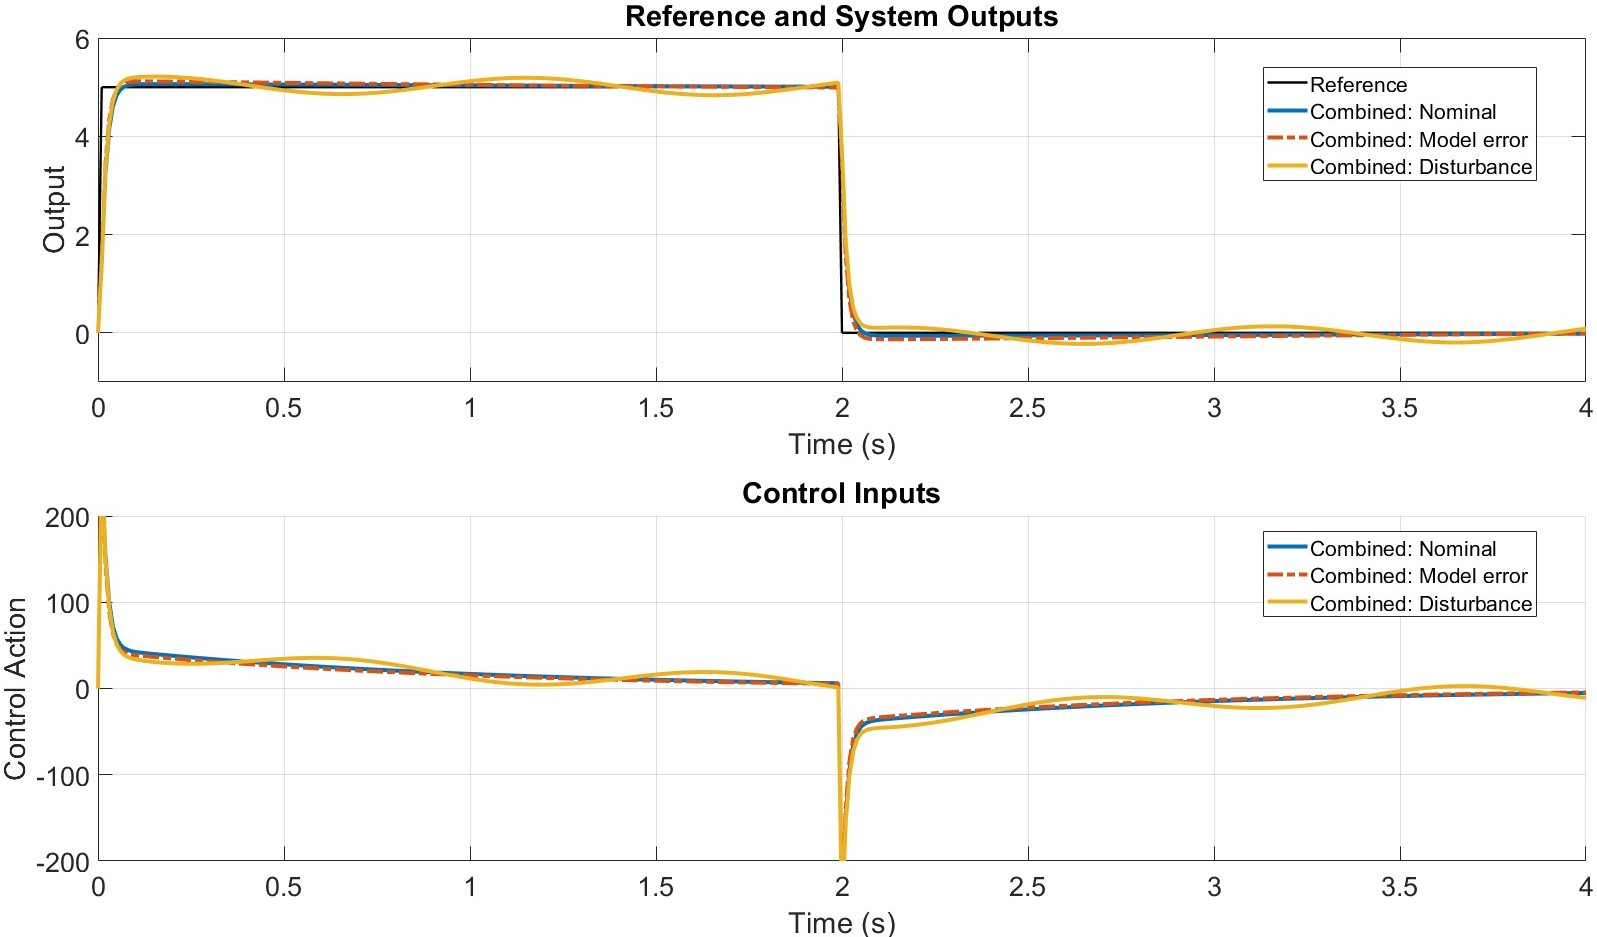
\includegraphics[width=\linewidth]{fig_control_configs/combined.jpg}
    \caption{Combined open- and close-loop control example: Reference \& Output} \label{fig_Combined}    
\end{figure}


\subsubsection{PID-F Controller}
Proportional-integral-derivative filtered controllers apply a control action which is the sum of three components: One proportional to the tracking error, another proportional to the integral of the error, and another proportional to a filtered derivative of the error. 

A discrete PID-F controller can be formulated as in the following equation:
\begin{equation}
    C(z) =  K_p + K_i \frac{T_s}{z-1} + K_d \frac{1}{T_f + \frac{T_s}{z-1}} 
\end{equation}

where $K_p$ is the proportional error gain, $K_i$ the integral error gain, $K_d$ the derivative error gain, $T_f$ the filter constant, and $T_s$ the sampling time.

The proportional component outputs a control action proportional to the error. If the proportional control results in steady-state error, the integral action will grow over time and correct for it. Additional integrators may be added to correct for steady-state error. The reasoning behind the derivative term is that, if there is a large variation of the error, the control action will immediately increase to counter it, rather than waiting for a large error (where the proportional action will kick in), or, even worse, for an accumulation of the error (where the integral action will kick in).


\subsubsection{Full State Feedback Control}
% \noindent
% \begin{minipage}{0.7\textwidth}\setlength{\parindent}{15pt}
In order to introduce the concept of state feedback control we'll start with a simple example. Consider the system in figure \ref{tikz_StateFeedbackControl_intro}:
\begin{figure}[H]
    \centering
    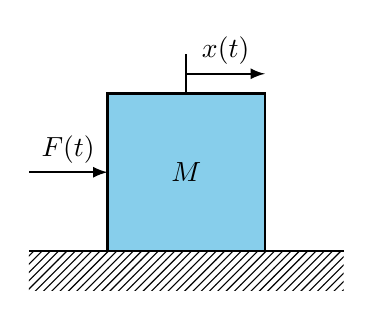
\begin{tikzpicture}[
        every node/.style={outer sep=0pt}, thick, % Set default node style and line thickness
        mass/.style={draw, thick}, % Define style for masses (rectangles)
        ground/.style={fill, pattern=north east lines, draw=none}] % Define style for ground

        \node[mass, minimum width=20mm, minimum height=20mm , fill=SkyBlue] (mT) {$M$}; % First mass 
        \draw[latex-] (mT.west) -- ++ (-10mm,0) node[midway, above]{$F(t)$}; % Force applied to mT
        \node[ground, minimum width=40mm, minimum height=5mm , below=0mm of mT ] (ground) {}; 
        \draw (ground.north west) -- (ground.north east); 

        %\draw[thin, dashed] (mT.south) -- (mT.south |- disp_line); % Align displacement lines
        \draw[latex-] ([yshift=2.5mm] mT.east |- mT.north) -- ++ (-1,0) node[above,midway]{$x(t)$} node[left, minimum height=5mm, minimum width=1mm ] (g'T){};
        \draw[thick] (g'T.north east) -- (g'T.south east); 
    \end{tikzpicture}
    \caption{Mass with a force acting on it. The force is the manipulated input, and the mass position is the output.} \label{tikz_StateFeedbackControl_intro}
\end{figure}

Which we'll attempt to stabilise using output feedback control with a proportional gain $k$ (shown in figure \ref{tikz_StateFeedbackControl_intro_outputControl}):
\begin{equation}
    F(t) = k _1\cdot ( x_{ref}(t) - x(t))
\end{equation}

Where the transfer function relating output to the reference is:
\begin{equation}
    \frac{x(t)}{x_{ref}(t)} = \frac{k_1}{s^2 + k_1}
\end{equation}

From which we find that the poles are on the imaginary axis ($s=\pm\sqrt{k_1}i$), the system will always oscillate, and it is not possible to stabilise the system using just output feedback control.

% \end{minipage}
% \hfill
% \begin{minipage}{0.26\textwidth}
%     \centering
%     \begin{tikzpicture}[
%         every node/.style={outer sep=0pt}, thick, % Set default node style and line thickness
%         mass/.style={draw, thick}, % Define style for masses (rectangles)
%         ground/.style={fill, pattern=north east lines, draw=none}] % Define style for ground

%         \node[mass, minimum width=20mm, minimum height=20mm , fill=SkyBlue] (mT) {$M$}; % First mass 
%         \draw[latex-] (mT.west) -- ++ (-10mm,0) node[midway, above]{$F(t)$}; % Force applied to mT
%         \node[ground, minimum width=40mm, minimum height=5mm , below=0mm of mT ] (ground) {}; 
%         \draw (ground.north west) -- (ground.north east); 

%         %\draw[thin, dashed] (mT.south) -- (mT.south |- disp_line); % Align displacement lines
%         \draw[latex-] ([yshift=2.5mm] mT.east |- mT.north) -- ++ (-1,0) node[above,midway]{$x(t)$} node[left, minimum height=5mm, minimum width=1mm ] (g'T){};
%         \draw[thick] (g'T.north east) -- (g'T.south east); 
%     \end{tikzpicture}
%     \caption{Mass with a force acting on it. The force is the manipulated input, and the mass position is the output.} \label{tikz_StateFeedbackControl_intro}
% \end{minipage}
% \end{figure}
% \vspace{-8mm}
% \begin{figure}[H]
    % \noindent
    % \begin{minipage}{0.52\textwidth}\setlength{\parindent}{15pt}

If, instead of using just the system output (position $x(t)$) as feedback, we use an additional state (in this case the velocity $\dot{x}$, shown in figure \ref{tikz_StateFeedbackControl_intro_stateControl}) for computing the control action:

\begin{figure}[H]
    \begin{minipage}{0.49\textwidth}
        \centering
        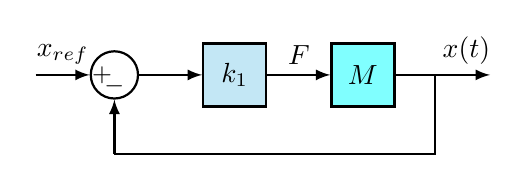
\begin{tikzpicture}[circ/.style = {draw, circle, minimum size=6mm, inner sep=0pt}, thick ]

        \node[circ]  (sum_r2) at (0,   0) {};
        \node[left=-1mm] at (sum_r2.center){\small $+$};
        \node[below=-1mm] at (sum_r2.center){\small $-$};

        \node[draw, fill=SkyBlue!50, minimum width=8mm, minimum height=8mm, right=8mm of sum_r2] (k) {$k_1$};% , label=above:{\parbox{17mm}{\centering closed-loop controller}}
        \node[draw, fill=Cyan!50, minimum width=8mm, minimum height=8mm , right=8mm of k      ] (M){$M$};% , label=above:{\parbox{15mm}{\centering system to control}}     

        \draw[-latex] (-10mm, 0) -- node[above]{$x_{ref}$}(sum_r2); %node[below]{reference} 
        \draw[-latex] (sum_r2) --  (k); % node[above]{\parbox{12mm}{\centering tracking error}}
        \draw[-latex] (k) --       node[above]{$F$} (M); % node[above]{\parbox{12mm}{\centering control action}}
        \draw[-latex] (M) --      node[above,at end, xshift=-3mm]{$x(t)$} ([xshift=12mm] M.east); % node[above]{output}                                  

        %--- Feedback: y branches back to sum_r2 bottom ---
        \coordinate (ybranch) at ([xshift=5mm] M.east);
        \draw (ybranch) --+(0, -1) -- (0, -1);
        \draw[-latex] (0, -1) -- (sum_r2.south);

        \end{tikzpicture}
        \caption{System from figure \ref{tikz_StateFeedbackControl_intro} with output feedback} \label{tikz_StateFeedbackControl_intro_outputControl} 
    \end{minipage}
    \hfill
    \begin{minipage}{0.49\textwidth}
        \centering
        \begin{tikzpicture}[circ/.style = {draw, circle, minimum size=6mm, inner sep=0pt}, thick ]
        \node[circ]  (sum1) at (0,   0) {};
        \node[left=-1mm] at (sum1.center){\small $+$};
        \node[below=-1mm] at (sum1.center){\small $-$};
            \draw[-latex] (-10mm, 0) -- node[above]{$x_{ref}$}(sum1); %node[below]{reference} 

        \node[draw, fill=SkyBlue!50, minimum width=8mm, minimum height=8mm, right=5mm of sum1] (k1) {$k_1$};
            \draw[-latex] (sum1) --  (k1); % node[above]{\parbox{12mm}{\centering tracking error}}

        \node[circ , right=5mm of k1]  (sum2) {};
        \node[left=-1mm] at (sum2.center){\small $+$};
        \node[below=-1mm] at (sum2.center){\small $-$};
                \draw[-latex] (k1) --  (sum2); % node[above]{\parbox{12mm}{\centering tracking error}}

        \node[draw, fill=Cyan!50, minimum width=8mm, minimum height=8mm , right=15mm of sum2 ] (M){$M$};

        \draw[-latex] (sum2) --   node[above]{$F$} (M); % node[above]{\parbox{12mm}{\centering control action}}
        \draw[-latex] (M) --      node[above,midway]{$x(t)$} ([xshift=8mm] M.east); % node[above]{output}                                  

        %--- Feedback: y branches back to sum_r2 bottom ---
        \coordinate (ybranch) at ([xshift=4mm] M.east);
        \draw (ybranch) --+(0, -1.6) -- (0, -1.6);
        \draw[-latex] (0, -1.6) -- (sum_r2.south);

        \node[draw, fill=SkyBlue!50, minimum width=8mm, minimum height=8mm, below=2mm of M , xshift=-12mm ] (k2) {$k_2$};
            \draw[-latex] (M.south) -- node[right]{$\dot{x}$}(M.south |- k2) -- (k2.east)  ; 
            \draw[-latex] (k2.west) -- (k2 -| sum2.south) -- (sum2.south);

        \end{tikzpicture}
        \caption{System from figure \ref{tikz_StateFeedbackControl_intro} with state feedback, where the states are position and velocity of the mass} \label{tikz_StateFeedbackControl_intro_stateControl} 
    \end{minipage}
\end{figure}

We have the following control law:
\begin{equation}
    F(t) = k_1 \cdot \left[ x_{ref}(t) - x(t)\right] - k_2 \dot{x}(t)
\end{equation}

And the closed-loop transfer function:
\begin{equation}
    \frac{x(t)}{x_{ref}(t)} = \frac{k_1}{s^2 + k_2 s + k_1}
\end{equation}

From which we can now see that the gains $k_1$ and $k_2$ may be chosen freely to place the closed-loop poles, $p_1$ and $p_2$, anywhere in the s-plane:
% \begin{equation}
%     s^2 + k_2 s + k_1 = (s-p_1)(s-p_2) \Longrightarrow  k_1 = p_1 p_2  \land k_2 = -p_1 - p_2
% \end{equation}
\begin{align}
    & s^2 + k_2 s + k_1 = (s-p_1)(s-p_2) \Longrightarrow \nonumber \\ 
    & \Longrightarrow  k_1 = p_1 p_2  \land k_2 = -p_1 - p_2
\end{align}

    % \end{minipage}
    % \hfill

\paragraph{Optimal Control}
Optimal control is precisely about designing the optimal state feedback controller gains. This is done by defining some performance index which is a function of the control action:
\begin{equation}
    J \left( x(t) , u(t) \right) = \int_{t_0}^{T} g\left( x(t) , u(t) \right) \, dt
\end{equation}

Where $x(t)$ represents the system states, and $u(t)$ the control action, of a given LTI system:
\begin{align} %\label{eq_LQR_performance_index}
    \dot{x}(t) =& A \, x(t) + B \, u(t) \\  %= f\left( x(t) , u(t)\right)
    y(t)       =&   C \, x(t)
\end{align} 

Usual performance indexes have a quadratic form to guarantee mathematical tractability. In section \ref{sec_Optimal_Control}, we'll want to find the optimal gains $k$ for reference tracking with LQR servo controller. An advantage of the linear quadratic optimal control method, over a pole-placement method, is that it provides a systematic way of computing the state feedback control gain matrix, guaranteeing a viable solution in terms of control action feasibility. To ensure the controller minimizes the tracking error we'll define the performance index:
\begin{equation} \label{eq_J_LQ}
    J \left( x(t) , u(t) \right)=\int_{0}^{t} \left( x^\intercal Q x + u^\intercal R u \right) \,dt 
\end{equation} 
by specifying matrices $Q$ and $R$, such that the minimization of the index mostly minimizes the state, or states, which somehow represent tracking error. In the case of the LQI controller in section \ref{sec_Optimal_Control}, the system will be augmented with a state which is the integral of the tracking error, and this is the state that will be weighted by matrix Q. In equation \eqref{eq_J_LQ}, the first term in the integrand affects state response, while the second affects control action.

Notice how the performance index integral in equation \ref{eq_J_LQ} is defined for a finite time. The optimal solution for the finite time control problem is $u(t)= k(t) x(t)$, with the gain vector $k(t)$ varying in time:
\begin{equation}
    k(t) = R^{-1} B^\intercal P(t)
\end{equation}

Which is computed by first solving $P(t)$ from the matrix differential Riccati equation:
\begin{equation}
    -\dot{P}(t) = A^\intercal P(t) + P(t) A - P(t) B R^{-1} B^\intercal P(t) + Q
\end{equation}

Alternatively, for the sake of simplicity, the performance index is defined for infinite time, and, in this case, as $t \rightarrow \infty$, the optimal control solution becomes the steady-state solution $u(t)= k x(t)$, with the gain vector $k$ and matrix $P$ becoming constant, making computation much faster and easier:
\begin{align}
    0 =& A^\intercal P + P A - P B R^{-1} B^\intercal P + Q \\
    k =& R^{-1} B^\intercal P
\end{align}
This solution is suboptimal, however.

\paragraph{Controllability}
For the existence of an optimal control vector, the system must be completely state controllable. A system is said to be state controllable if it is possible to construct a finite control action that will transfer an initial state to any final state in a finite time interval. If every state is controllable, then the system is said to be completely state controllable \citep{Sa_da_Costa}. 

It is important to note that controllability is not a property of the system, but, instead, a property of the state space representation, and is affected only by the state and input matrices, $A$ and $B$, respectively \citep{Botto}.

\paragraph{Observability}
In order to implement state feedback control one must, obviously, know the states. The concept of observability is useful in solving the problem of reconstructing unmeasurable state variables from measurable variables in the minimum possible length of time. A system is said to be completely observable if every state can be determined from the observation of the system output over a finite time interval. The system is, therefore, completely observable if every transition of the state eventually affects every element of the output vector \citep{Sa_da_Costa}.

It is important to note that observability, like controllability, is not a property of the system, but a property of the state space representation, and is affected only by the state and output matrices, $A$ and $C$, respectively \citep{Botto}.

\paragraph{State Observers}
A state observer estimates system states from measurements of inputs and outputs of a system. This is done such that state feedback control can be applied to systems with unmeasurable states. In section \ref{sec_LQG Servo Controller} a stationary Kalman filter %(isn't recursively updated)
is implemented to estimate the systems states, mixing a priori information from the identified system model with the measured output to compute an estimate of the states.

For a given plant:
\begin{align}   
    \dot{x} =& A x + B u +  w \\
    y =& C x + v
\end{align}

Where $w(t)$ and $v(t)$ are Gaussian white noise processes with covariance matrices:
\begin{align}
    Q_n =& E\left[ w w^\intercal\right] \\
    R_n =& E\left[ v v^\intercal\right] 
\end{align}

The Kalman estimator:
\begin{align}   
    \dot{\widehat{x}} =& A \widehat{x} + B u + L_K \left( y - C \widehat{x} \right) \\
    \widehat{y} =& C \widehat{x} 
\end{align}

Computes state estimate $\widehat{x}(t)$ that minimizes the steady-state error covariance:
\begin{equation}
    P = \lim_{t \rightarrow \infty} E \left( (x - \widehat{x}) (x - \widehat{x})^\intercal \right)
\end{equation}

Where the filter gain $L_K$ is given by:
\begin{equation}
    L_K = P C^\intercal R^{-1}_n
\end{equation}

Where $P$ is the solution of the algebraic Riccati equation:
\begin{equation}
    A P + P A^\intercal + B Q_n B^\intercal - P C^\intercal R^{-1}_n C P = 0
\end{equation}

Matrices $Q_n$ and $R_n$ can be used to tune the observer, biasing the states estimates towards what our model of system expects (done when the measurements are unreliable), or what the sensors are reading (done when the model is not exact).

\section{Identification in Closed-Loop Systems} \label{Identification in Closed-Loop Systems}
%\hspace{\parindent} 
Many systems operate under feedback control due to required safety of operation (as is the case of LNEC's shaking tables), or to unstable behaviour of the plant meaning that experiments can only be performed under presence of a stabilizing controller. Biological and economic systems operate only under closed-loop conditions, and it is not even possible to remove the feedback loop. On occasion, performing experiments in closed loop may be preferable to operating in open loop, such as a situation in which the objective of the identification is to design a better controller, then, the dynamics of the plant in closed loop with the original controller may be more relevant than the open loop for designing an improved controller \citep{VanDenHof2020}. 

In section \ref{Nonparametric Modelling} it will be shown that the identification of systems working in closed loop can be problematic under certain conditions, with a specific focus on nonparametric modelling by spectral analysis, as this is the method currently used at LNEC when synthesizing adapted drivers for the shaking tables. In section \ref{Two-Stage Method} a method for circumventing the issues introduced by the feedback loop will be presented. These segments are specially influenced by the works of \cite{VanDenHof2020} and \cite{Soderstrom_Stoica},

%\pagebreak
\subsection{ Closed Loop System Setup} %(Section \ref{Identification in Closed-Loop Systems})
In this section we'll consider the closed-loop discrete-time system represented in figure \ref{tikz_general_CL_sys}, and restrict ourselves to the case of SISO systems (single-input single-output):

\begin{figure}[H]
    \centering
        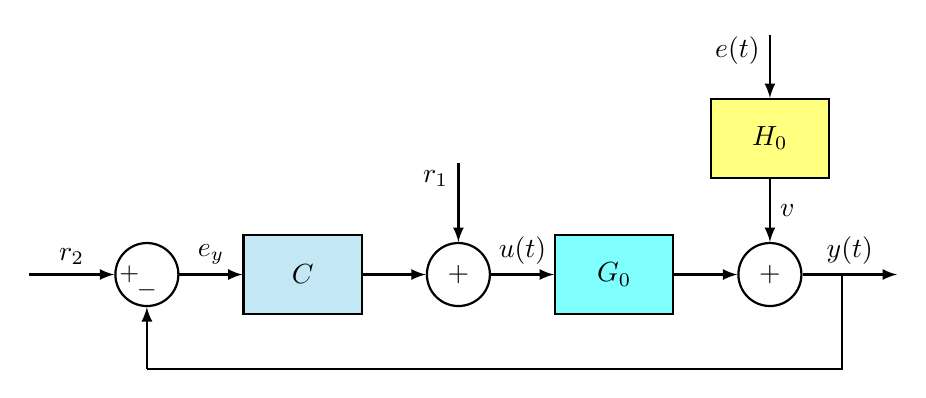
\begin{tikzpicture}[circ/.style = {draw, circle, minimum size=8mm, inner sep=0pt}, thick ]
        % sum_r2
        \node[circ]  (sum_r2) at (0,   0) {};
        \node[left=-1pt] at (sum_r2.center){\small $+$};
        \node[below=-1pt] at (sum_r2.center){\small $-$};

        % C
        \node[draw, fill=SkyBlue!50, minimum width=15mm, minimum height=10mm, right=8mm of sum_r2 ] (C) {$C$};

        % sum_r1
        \node[circ , right=8mm of C ]  (sum_r1) {$+$};

        % G0
        \node[draw, fill=Cyan!50, minimum width=15mm, minimum height=10mm , right=8mm of sum_r1 ] (G0)    {$G_0$};

        % sum_v
        \node[circ, , right=8mm of G0 ]  (sum_v) {$+$};

        % H0
        \node[draw, fill=Yellow!50, minimum width=15mm, minimum height=10mm, above=8mm of sum_v ] (H0)  {$H_0$};

        %--- Input r2 ---
        \draw[-latex] (-1.5, 0) -- node[above]{$r_2$} (sum_r2);

        %--- sum_r2 -> C -> sum_r1 ---
        \draw[-latex] (sum_r2) -- node[above]{$e_y$} (C);
        \draw[-latex] (C) -- (sum_r1);

        %--- r1 drops into sum_r1 from above ---
        \draw[-latex] ([yshift=10mm]sum_r1.north) node[left ,yshift=-2mm]{$r_1$} -- (sum_r1);

        %--- sum_r1 -> G0 ---
        \draw[-latex] (sum_r1) -- node[above]{$u(t)$} (G0);

        %--- G0 -> sum_v ---
        \draw[-latex] (G0) -- (sum_v);

        %--- e -> H0 -> v -> sum_v ---
        \draw[-latex] ([yshift=8mm]H0.north) node[left,yshift=-2mm]{$e(t)$} -- (H0);
        \draw[-latex] (H0) -- node[right]{$v$} (sum_v);

        %--- sum_v -> y output ---
        \draw[-latex] (sum_v) -- node[above]{$y(t)$} ([xshift=12mm] sum_v.east);

        %--- Feedback: y branches back to sum_r2 bottom ---
        \coordinate (ybranch) at ([xshift=5mm] sum_v.east);
        \draw (ybranch) --+(0, -1.2) -- (0, -1.2);
        \draw[-latex] (0, -1.2) -- (sum_r2.south);

        \end{tikzpicture}
    \caption{Closed-loop System}%, with position $X_{ref}$ as input and force applied to the platen $F_P$ as output.
    \label{tikz_general_CL_sys} 
\end{figure}

For the system in figure \ref{tikz_general_CL_sys}, the following equations are derived:
\begin{align} %\begin{numcases}{}
    y(t) &= G_0 \cdot u(t) + H_0 \cdot e(t) \label{eq_y_original_CL} \\ 
    u(t) &= r_1(t) + C \cdot r_2(t) - C \cdot y(t) \label{eq_u_original_CL}
\end{align} %\end{numcases}

In the whole of section \ref{Identification in Closed-Loop Systems}, for the examples presented, and, unless stated otherwise, we'll consider the following conditions:
\begin{itemize}
    \item $r_{1}(t)$, $r_{2}(t)$ (referred to as reference/set point signals), $e(t)$(referred to as disturbance or noise) are Gaussian white noise data sequences generated with MATLAB's \emph{wgn} function, with power set to 1
    \item $C(z)$ is the system controller, which will vary between examples
    \item $G_{0}(z) = \frac{1}{1-1.6z^{-1}+0.89z^{-2}}$ is the plant
    \item $H_{0}(z) = \frac{1 - 1.56z^{-1} + 1.045z^{-2} -0.3338z^{-3}}{1 - 2.35z^{-1} + 2.09z^{-2} -0.6675z^{-3}}$ is the noise model
\end{itemize}

We'll start by transforming the system equations. The reasons why this is of interest will become apparent soon. Firstly, for simplicity's sake, we'll substitute $e(t)$  in equation \eqref{eq_y_original_CL}:
\begin{equation}
    v(t) = H_{0}(z) \cdot e(t) \Longrightarrow y(t) = G_0 \cdot u(t) + v(t) \label{eq_v_H0e}
\end{equation}

By introducing the sensitivity transfer function:
\begin{equation}
    S_0 = \frac{1}{1 + G_0 \cdot C} \label{eq_S0}
\end{equation}

Rewriting equations \eqref{eq_y_original_CL} and \eqref{eq_u_original_CL} using relations \eqref{eq_v_H0e} and \eqref{eq_S0}, we get:
\begin{align}
    y(t) &= S_0 G_0 \cdot r_1(t) + S_0 G_0 C \cdot r_2(t)  + S_0 \cdot v(t) \label{eq_y_transformed_CL} \\  
         &= H_{yr_{1}} \cdot r_1(t) + H_{yr_{2}} \cdot r_2(t) + H_{yv} \cdot v(t) \nonumber \\[2mm]
    u(t) &= S_0 \cdot r_1(t) + S_0 C \cdot r_2(t) - S_{0}C \cdot v(t)   \label{eq_u_transformed_CL}  \\
         &= H_{ur_{1}} \cdot r_1(t) + H_{ur_{2}} \cdot r_2(t) + H_{uv} \cdot v(t) \nonumber
 \end{align}

The block diagram resulting from these reworked equations is shown in Figure \ref{transformed_CL_sys}:
\begin{figure}[H]
    \centering
        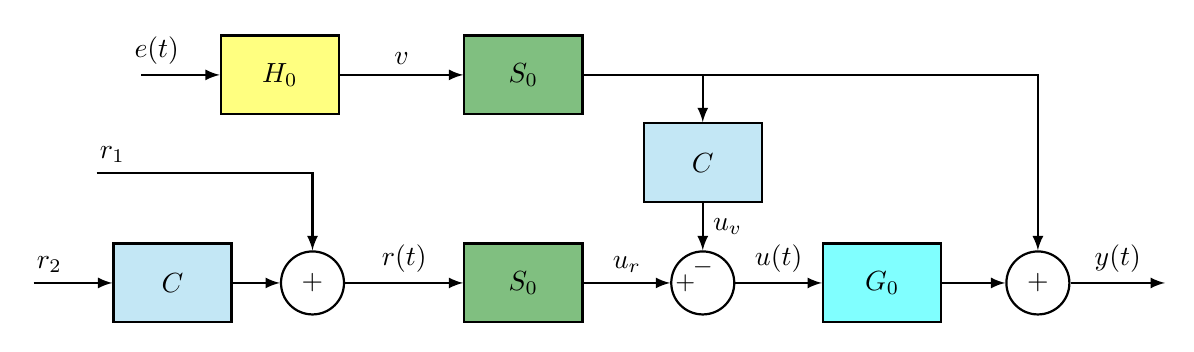
\begin{tikzpicture}[circ/.style = {draw, circle, minimum size=8mm, inner sep=0pt}, thick ]
        % S0 -  Referential Origin
        \node[draw, fill=Green!50, minimum width=15mm, minimum height=10mm ] (S0) at (0,0){$S_0$};

        % sum_u
        \node[circ , right=11mm of S0 ]  (sum_u) {};
        \node[left=-1pt] at (sum_u.center){\small $+$};
        \node[above=-1pt] at (sum_u.center){\small $-$};

        % G0
        \node[draw, fill=Cyan!50, minimum width=15mm, minimum height=10mm , right=11mm of sum_u ] (G0)    {$G_0$};

        % sum_y
        \node[circ,  right=8mm of G0 ]  (sum_y) {$+$};

        % S0C
        \node[draw, fill=SkyBlue!50, minimum width=15mm, minimum height=10mm, above=6mm of sum_u ] (C_v)  {$C$};

        % sum_r % r = r1 + C*r2
        \node[circ, , left=15mm of S0 ]  (sum_r) {$+$};

        % C
        \node[draw, fill=SkyBlue!50, minimum width=15mm, minimum height=10mm, left=6mm of sum_r ] (C) {$C$};

        % %--- Input r1 ---
        \draw [-latex] ([yshift=14mm, xshift=-2mm]C.west) -- node[above,at start, xshift=2mm]{$r_1$}([yshift=14mm] C.west -| sum_r) -- (sum_r.north);

        % %--- Input r2 ---
        \draw[-latex] ([xshift=-10mm]C.west) -- node[above,at start, xshift=2mm]{$r_2$} (C);

        % %--- Input to sum_r ---
        \draw[-latex] (C) -- (sum_r);

        %--- r -> S0
        % \draw[-latex] ([xshift=-10mm]S0.west) -- node[left, yshift=2mm]{$r(t)$} (S0);
        \draw[-latex] (sum_r.east) -- node[above]{$r(t)$} (S0);

        %--- S0 -> u_r
        \draw[-latex] (S0) -- node[above] {$u_r$} (sum_u);
        % %--- r1 drops into sum_u from above ---
        % \draw[-latex] ([yshift=10mm]sum_u.north) node[left ,yshift=-2mm]{$r_1$} -- (sum_u);

        %--- sum_u -> G0 ---
        \draw[-latex] (sum_u) -- node[above]{$u(t)$} (G0);

        %--- G0 -> sum_y ---
        \draw[-latex] (G0) -- (sum_y);

        %--- sum_y -> y output ---
        \draw[-latex] (sum_y) -- node[above]{$y(t)$} ([xshift=12mm] sum_y.east);

        % H0
        \coordinate (ybranch) at ([yshift=6mm] C_v.north);
        \node[draw, fill=Yellow!50, minimum width=15mm, minimum height=10mm] (H0) at (sum_r.west |- ybranch) {$H_0$};

        % %--- Input e ---
        \draw[-latex] ([xshift=-10mm]H0.west) -- node[above,at start, xshift=2mm]{$e(t)$} (H0);

        % another S0 
        \node[draw, fill=Green!50,, minimum width=15mm, minimum height=10mm ] (S0_v) at (H0 -| S0) {$S_0$};

        %--- v -> C_v -> u_v -> sum_y ---
        \draw[-latex] (C_v) -- node[right]{$u_v$} (sum_u);

        % %--- v branches to sum_y
        \draw[-latex] (H0.east) -- node[above]{$v$}(S0_v);
        \draw[-latex] (S0_v) -- (S0_v -| C_v) -- (C_v.north);
        \draw[-latex] (S0_v -| C_v) -- (S0_v -| sum_y) -- (sum_y.north);



        \end{tikzpicture}
    \caption{The closed-loop system is reformulated into pseudo-open loop form by reworking the equations. The control action, $u$, is now decomposed in two: the noise free control action, $u_r$(resulting from the reference, $r$) and the corrupted control action, $u_v$(resulting from disturbance on the output being fed back to the controller).}
    \label{transformed_CL_sys} 
\end{figure}


\subsection{Nonparametric Modelling by Spectral Analysis}\label{Nonparametric Modelling}
\subsubsection{Why it works in open-loop}

For our system, taking the spectral density $\Phi_{yu}$, we get:
\begin{equation}
    \Phi_{yu}(\omega) =  G_{0}(e^{i\omega}) \, \Phi_{u}(\omega) + H_{0}(e^{i\omega}) \, \Phi_{eu}(\omega)
\end{equation}

However, if we consider an open loop system as in figure \ref{tikz_general_open_loop_sys}:
\begin{figure}[H]
    \centering
        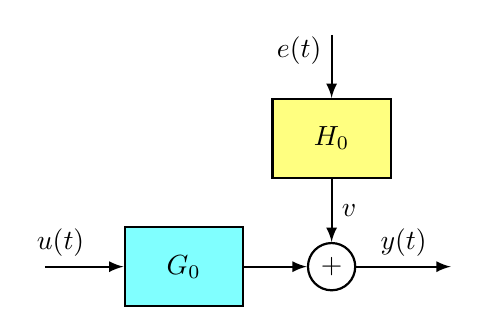
\begin{tikzpicture}[circ/.style = {draw, circle, minimum size=6mm, inner sep=0pt}, thick ]

        % G0
        \node[draw, fill=Cyan!50, minimum width=15mm, minimum height=10mm  ] (G0) at (0,0)   {$G_0$};

        % sum_v
        \node[circ, right=8mm of G0 ]  (sum_v) {$+$};

        % H0
        \node[draw, fill=Yellow!50, minimum width=15mm, minimum height=10mm, above=8mm of sum_v ] (H0)  {$H_0$};

        %--- G0 -> sum_v ---
        \draw[-latex] (G0) -- (sum_v);

        %--- e -> H0 -> v -> sum_v ---
        \draw[-latex] ([yshift=8mm]H0.north) node[left,yshift=-2mm]{$e(t)$} -- (H0);
        \draw[-latex] (H0) -- node[right]{$v$} (sum_v);

        %--- sum_v -> y output ---
        \draw[-latex] (sum_v) -- node[above]{$y(t)$} ([xshift=12mm] sum_v.east);

        %--- sum_r1 -> G0 ---
        \draw[-latex] ([xshift=-10mm]G0.west) -- node[above,at start, xshift=2mm]{$u(t)$} (G0);

        \end{tikzpicture}
        \caption{Open-loop System}\label{tikz_general_open_loop_sys} 
\end{figure}
where the output $y$ (which contains the disturbance $e$) is not being fed back into the plant, then, given the fact that $e$ and $u$ are uncorrelated (meaning $\Phi_{eu}(\omega) = 0$), our plant can be estimated directly by estimating the spectral densities:
\begin{equation}
    \widehat{G}(e^{i\omega}) = \frac{\widehat{\Phi}_{yu}(\omega)}{\widehat{\Phi}_{u}(\omega)} \label{eq_G_spectral_estimate_open_loop}
\end{equation}


\subsubsection{The problem in closed-loop}
Applying the same technique for our closed loop system (figure \ref{tikz_general_CL_sys}), from equations \eqref{eq_y_transformed_CL} and \eqref{eq_u_transformed_CL}, we find:
\begin{align}
\Phi_{u}(\omega) =& \left|H_{ur_{1}}\right|^2 \Phi_{r_{1}} + \left|H_{ur_{2}}\right|^2 \Phi_{r_{2}} + \left|H_{uv}\right|^2 \Phi_{v} \nonumber\\ 
                 =& \left|S_{0}\right|^2 \Phi_{r_{1}} + \left|S_{0} C\right|^2 \Phi_{r_{2}} + \left|- S_{0} C\right|^2 \Phi_{v} \nonumber \\
                 =& \left|S_{0}\right|^2 \left[\Phi_{r_{1}} + \left| C\right|^2 \Phi_{r_{2}} + \left|C\right|^2 \Phi_{v} \right] \\[2mm]
                %  =& \left|S_{0}(e^{i\omega})\right|^2 \left[\Phi_{r_{1}}(\omega) + \left| C(e^{i\omega})\right|^2 \Phi_{r_{2}}(\omega) + \left|C(e^{i\omega})\right|^2 \Phi_{v}(\omega) \right] \\[2mm]
\Phi_{yu}(\omega) =& \, H_{yr_{1}} H^{*}_{ur_{1}} \Phi_{r_{1}} + H_{yr_{2}} H^{*}_{ur_{2}} \Phi_{r_{2}} + H_{yv}{} H^{*}_{uv} \Phi_{v} \nonumber \\ 
                  =& \, S_0 G_0 \cdot S^{*}_{0} \, \Phi_{r_{1}} + S_0 G_0 C \cdot \left(S_0 C\right)^{*} \Phi_{r_{2}} + S_0 \cdot \left(-S_0 C\right)^{*} \Phi_{v} \nonumber \\ 
                  =&\left|S_{0}\right|^2  \left[ G_0 \,  \Phi_{r_{1}} +  G_0 \left|C\right|^2 \Phi_{r_{2}} - C^{*} \, \Phi_{v} \right] \\[2mm]
\widehat{G}(e^{i\omega}) =& \, \frac{\Phi_{yu}(\omega)}{\Phi_{u}(\omega)} \, =\, \frac{G_0 \,  \Phi_{r_{1}} +  G_0 \left|C\right|^2 \Phi_{r_{2}} - C^{*} \, \Phi_{v} }{ \Phi_{r_{1}} + \left| C\right|^2 \Phi_{r_{2}} + \left|C\right|^2 \Phi_{v} } \label{eq_G_spectral_estimate}
\end{align}

From equation \eqref{eq_G_spectral_estimate} we can verify that, if $C(z)=0$, then we simply have the open-loop case as in equation \eqref{eq_G_spectral_estimate_open_loop}:
\begin{equation}
    C(z)=0  \quad \Longrightarrow \widehat{G}(e^{i\omega}) =\, \frac{G_0 \,  \Phi_{r_{1}} +  0 - 0 }{ \Phi_{r_{1}} + 0 + 0} =\, \frac{G_{0}(e^{i\omega}) \,  \Phi_{r_{1}}(\omega) }{ \Phi_{r_{1}}(\omega) } = \, G_{0}(e^{i\omega})   
\end{equation}

What's more interesting, though, is the closed-loop scenario, so we'll consider $C(z) \neq 0$. From equation \eqref{eq_G_spectral_estimate} we can verify that, if the disturbance $v$ is very small ($\Phi_{v}(\omega) \longrightarrow 0 $), the identification of the plant's true dynamics is possible:
\begin{align}
    \Phi_{v}(\omega) \longrightarrow 0  \; & \Longrightarrow \widehat{G}(e^{i\omega}) =\, \frac{G_0 \,  \Phi_{r_{1}} +  G_0 \left|C\right|^2 \Phi_{r_{2}} - 0 }{ \Phi_{r_{1}} + \left| C\right|^2 \Phi_{r_{2}} + 0 } = \, \frac{ G_0 \cdot \left[\Phi_{r_{1}} + \left|C\right|^2 \Phi_{r_{2}}\right] }{ \quad \Phi_{r_{1}} + \left| C\right|^2 \Phi_{r_{2}}} = \, G_{0}(e^{i\omega})   
\end{align}

But if the disturbance $v$ is very large compared to the reference signals $r_1$ and $r_2$, then it results:
\begin{equation}
    \frac{\Phi_{r_{1}}(\omega)}{\Phi_{v}(\omega)} \longrightarrow 0 \; , \frac{\Phi_{r_{2}}(\omega)}{\Phi_{v}(\omega)} \longrightarrow 0 \; \Longrightarrow \widehat{G}(e^{i\omega}) =\,\frac{0 +  0 - C^{*} }{ 0 + 0 + \left|C\right|^2 } = \frac{- C^{*}}{C \cdot C^{*}} = \frac{-1}{C(e^{i\omega})}
\end{equation}

So it's clear that the spectral analysis method in closed-loop always results in biased estimates of the plant, with the identified model $\widehat{G}$ being somewhere between $G_0$ and $\frac{-1}{C}$, as weighed by the spectral density of each signal and the controller.

\subsubsection{Remark on parametric modelling}
Parametric modelling via direct identification, as shown in \cite{VanDenHof2020}, can yield consistent plant estimates, but only under restrictive conditions: full-order models must be used, the noise structure must be accurately modelled, and either a sufficiently exciting external signal $r$ must be present, or a sufficiently high-order controller must be employed, or the controller must switch settings during the experiment. Indirect and joint input-output methods, while theoretically sound, require more complex parameterisations and additional estimation steps, making them less practical in many settings. The parametric identification method introduced in Section \ref{Two-Stage Method} addresses these closed-loop identification challenges while remaining straightforward to implement.

\subsection{Two-Stage Method for Closed Loop Identification}\label{Two-Stage Method}
\subsubsection{Introduction}
\hspace{\parindent}The two-stage method is introduced in Van den Hof and Schrama (1993). It is of special interest compared to other parametric modelling approaches since it deals with the consistency problem of identifying $G_0$ without having to accurately model $H_0$, but also due to its simplicity and flexibility. It does not impose restrictions on the controller, which can be of any order, nonlinear, and even of variable structure (as in sliding mode control), etc., nor does it require prior knowledge of its dynamics. It also does not require complex parametrized models or solving additional equations when reduced order models are desired.

The simplicity results from the fact that the procedure comes down to two standard open-loop identification steps. This approach works on the principle that it is possible to decompose the control action, $u$, in two components: the noise free control action, $u_r$ which results from the reference, $r$; and the corrupted control action, $u_v$ which results from the disturbance $v$ on the output being fed back to the control.
\begin{align}
    u(t) =& \, u_r + u_v  \\
         =& \, S_0 \left[ r_{1}(t) + C r_{2}(t) \right] - S_0 C v(t) 
\end{align}

If this holds, it is then possible to estimate $G_0$, not from $u$ (which is corrupted), but from $y$ and $u_r$, since $u_r$ is uncorrelated to $v$ and $u_v$:
\begin{align}
    y(t) =& \, G_0 u(t) + v(t) \nonumber \\ 
         =& \, G_0 \left[u_{r}(t) + u_{v}(t) \right] + v(t)  \nonumber\\ 
         =& \, G_0 u_{r}(t) + \left[G_0 u_v(t) + v(t) \right]
\end{align}

\subsubsection{The Method} 
\paragraph{Estimating the sensitivity function}

If we mind equation \ref{eq_u_transformed_CL}, condensing the external reference signals in a single variable, it  results:
\begin{equation}
    r(t) = r_1(t) + C(z) \cdot r_2(t)
\end{equation} 

And, rewriting the equation, we get:
\begin{equation}
    u(t) = S_{0} \cdot r(t) - S_{0} C \cdot v(t) 
\end{equation}

Now the reason for formulating the problem using the sensitivity function becomes apparent, due to the fact that $r(t)$ and $v(t)$ are uncorrelated, $S_0$ can be estimated in a usual open-loop way from the measured $u(t)$ signal, and the known reference signal $r(t)$. This is the first step:
\begin{equation}
    \widehat{S_{0}}(z) = \frac{u(t)}{r(t)}
\end{equation}

\paragraph{Reconstructing the noise-free control action}
From the known reference signal $r(t)$, the estimated sensitivity function can be used to reconstruct the noise-free control action $\widehat{u}_{r}(t)$:
\begin{equation}
    \widehat{u}_{r}(t) = \widehat{S_{0}}(z) \cdot r(t)
\end{equation}

Since the sensitivity function is used here solely to reconstruct the noise-free control action, the model for the sensitivity function may be of arbitrarily high order. However, restricting variance, and thus reducing the number of parameters, may still be of interest.

\paragraph{Estimating the plant}
From the computed noise-free control action, $\widehat{u}_{r}$, and measured system output $y$, it is now possible to estimate the plant: % (which is uncorrelated with $v$)
\begin{equation}
    \widehat{G}(z) = \, \frac{y(t)}{\widehat{u}_{r}(t)}
\end{equation}


\subsection{Example: Comparing Closed-Loop Identification Methods}

The following examples display the identification results obtained with the methods discussed in sections \ref{Nonparametric Modelling} and \ref{Two-Stage Method}. To illustrate the effects of the controller in the identification results, in the first example the controller was set to a proportional gain, and in the second example, to a weighted sum of two delays. For each controller, two scenarios are shown: one where the ratio of disturbance to external excitation (reference signal) is moderate, and another where the disturbance is more severe. 

For this section, consider the following:
\begin{itemize}
    \item A data sequence containing 32768 points was used;
    \item  $r_1(t) = 0$, where the tracking error ($e_y = r_2 - y$) is what is input to the controller, as this mimics the setup at LNEC;
    \item The data sequences $r_{2}(t)$ and $e_0(t)$ for the pairs of examples are the same, with the noise input $e(t)$ in each one resulting from a scaling of $e_0(t)$:  $e(t) = k \cdot e_0(t)$;
    \item In figures \ref{fig_two_stage/example/K5_noise01} and \ref{fig_two_stage/example/K5_noise1}, the controller was set to $C(z)=5$;
    \item In figures \ref{fig_two_stage/example/noise005} and \ref{fig_two_stage/example/noise08}, the controller was set to $C(z)=0.5 \cdot (z^{-1} + 0.8 z^{-2})$ .
\end{itemize}  

%\subsubsection[Controller set as \texorpdfstring{$C(z) = 5$}{C(z) = 5}]{Controller set as \texorpdfstring{$C(z) = 5$}{C(z) = 5}}
\begin{figure}[H]
\begin{subfigure}{0.47\textwidth}
    \centering
    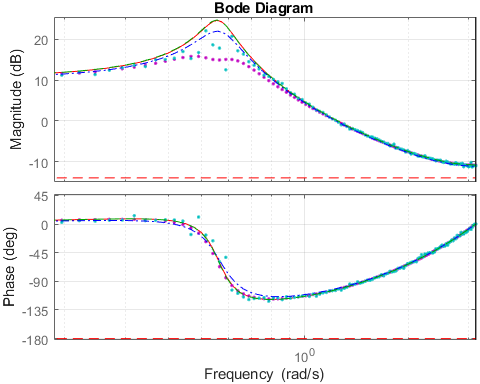
\includegraphics[width=\linewidth]{two_stage/example/K5_noise01.png}
    \caption{$C(z)=5$ and $e(t)=0.1 \cdot e_0(t)$}
    \label{fig_two_stage/example/K5_noise01}    
\end{subfigure}
\hfill
\begin{subfigure}{0.52\textwidth}
    \centering
    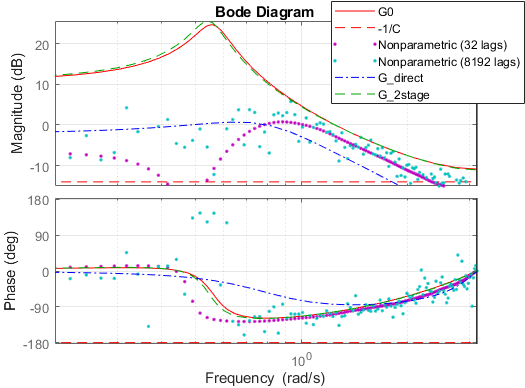
\includegraphics[width=\linewidth]{two_stage/example/K5_noise1.png}
    \caption{$C(z)=5$ and $e(t)=1 \cdot e_0(t)$}
    \label{fig_two_stage/example/K5_noise1}
\end{subfigure}
\\[5mm]
\begin{subfigure}{0.49\textwidth}
    \centering
    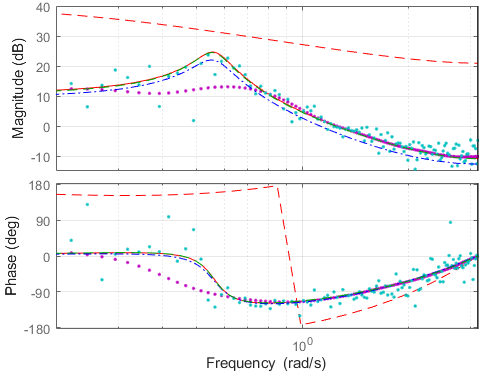
\includegraphics[width=\linewidth]{two_stage/example/noise005.png}
    \caption{$C(z)=0.5 \cdot (z^{-1} + 0.8 z^{-2})$ and $e(t)=0.05 \cdot e_0(t)$}
    \label{fig_two_stage/example/noise005}    
\end{subfigure}
\hfill
\begin{subfigure}{0.49\textwidth}
    \centering
    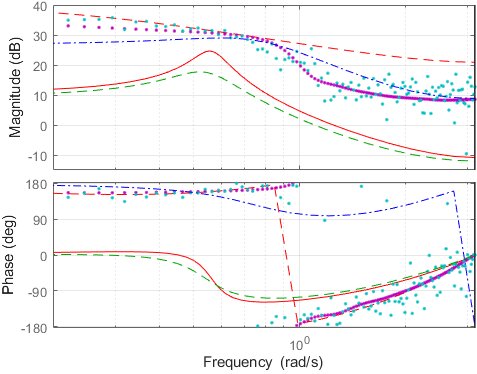
\includegraphics[width=\linewidth]{two_stage/example/noise08.png}
    \caption{$C(z)=0.5 \cdot (z^{-1} + 0.8 z^{-2})$ and $e(t)=0.8 \cdot e_0(t)$}
    \label{fig_two_stage/example/noise08}
\end{subfigure}
\caption{Bode plot of identification results with different controllers $C(z)$ and output disturbances $e(t)$}
\end{figure}

The figure on the left shows the results of the identification with some noise, but not too severe, and here we can see that the results of the non-parametric models are very sensitive to windowing. On the one hand, a smaller window (pink dots) results in a model that is less sensitive to variations in the data, but with a high bias. A larger window (light blue dots) captures the dynamics of the system well, but suffers from high variance. As for parametric methods, we see that the two-stage method achieves excellent identification (green line, completely superimposed on the ideal model, in red), while the direct method fails. In the figure on the right, we see an example with extreme noise, such that the models obtained by non-parametric methods and the direct method are approaching the inverse of the controller. Here, the two-stage method shines by giving still acceptable results.


\chapter[Evaluating Controller Performance in Simulation]{Evaluating Controller Performance in Simulation Environment for LNEC's \\ Uniaxial Shaking Table}\label{Evaluating Controller Performance in Simulation Environment}

In this chapter a model of LNEC's uniaxial shaking table (section \ref{Modelling Shaking Table Dynamics}) is used to evaluate the performance of three control strategies: the OLI method currently in use at LNEC (in section \ref{sec_LNEC_method}), tuned PID-F controllers (in section \ref{sec_Tuned_PID-F}), and optimal controllers (in section \ref{sec_Optimal_Control}).

\section{A Model of LNEC's Uniaxial Shaking Table}\label{Modelling Shaking Table Dynamics}
%\chapter{Modelação Matemática}
%Os modelos devem ser implementados em Matlab/Simulink e complementados com funções, scripts e interfaces que facilitem a parametrização, cálculo de propriedades (como modos de vibração), análise e simulação com diferentes tipos de entradas (sinais sinusoidais, ondas quadradas e inputs externos como sinais sísmicos).

\subsection{Previous Works}

In \cite{oliveira2015} a complete schematic representation of the ST1D, with a coupled 2DOF system, instrumentation, control, and acquisition system can be found (figure \ref{fig_schematic_st1d_Fernando}):
\begin{figure}[H]
    \centering
    \fbox{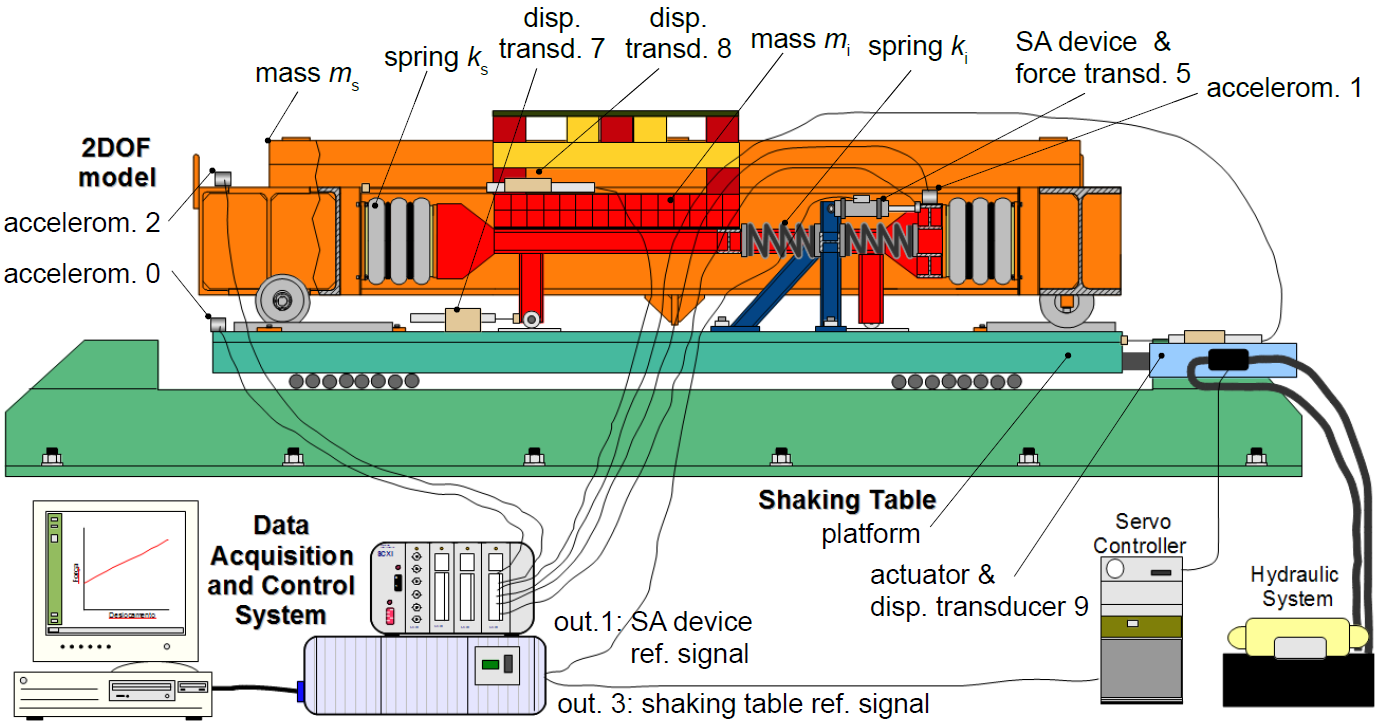
\includegraphics[width=0.95\textwidth]{Intro/schematic_st1d_Fernando.png}}
    \caption{Complete schematic representation of uniaxial shaking table (ST1D) with a coupled 2DOF system \citep{oliveira2015}}
    \label{fig_schematic_st1d_Fernando}
\end{figure}

In \citet{tekeste2021}, through a dedicated  experimental campaign to characterise the dynamic behaviour of the shaking table, a model for the ST1D with a coupled 1DOF system is devised by parametrizing linearized analytical models for each of its components (controller, servo valve, hydraulic actuator, platen mass, and total damping). This model is shown in figure \ref{fig_Tekeste_block_diagram}, and the parameters are presented in table \ref{tab:parameters}, and are the ones which will be used in all simulation studies.

\begin{figure}[H]
    \centering
    \fbox{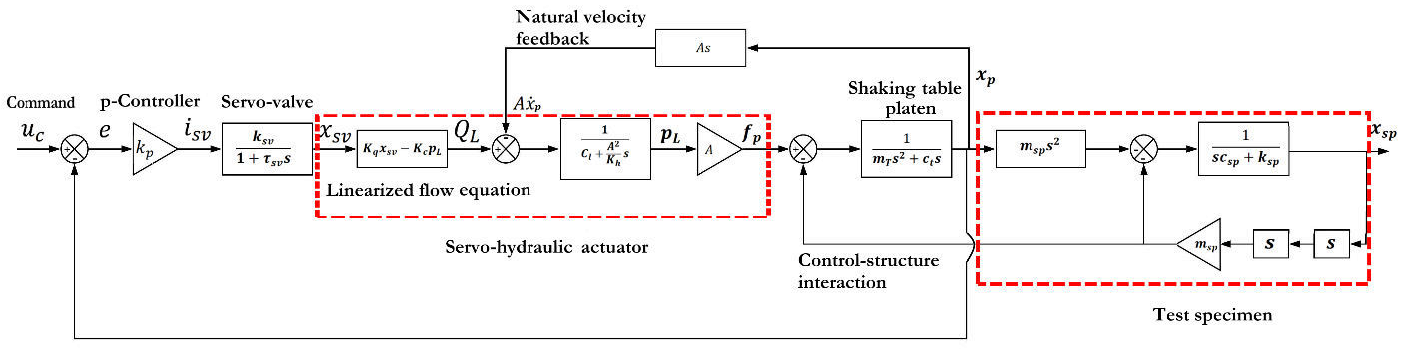
\includegraphics[width=0.98\linewidth]{Modelling/Gidewon_block_diagram.png}}
    \caption{Schematic diagram of a shaking table system with payload rigidly attached \citep{tekeste2021}}
    \label{fig_Tekeste_block_diagram}
\end{figure}

\begin{table}[H]
\centering
\caption{ST1D model parameters \citep{tekeste2021}}
\begin{tabular}{c  l  l }
\hline
\textbf{Symbol} & \textbf{Description} & \textbf{Value} \\ \hline
$k_p$ & Proportional gain of the controller & $1.2993 \, \text{V/cm}$ \\ \hline
$\tau_{sv}$ & Time-delay parameter of the servo-valve transfer function & $0.0246 \, \text{s}$ \\ \hline
$k_{sv}$ & Servo-valve gain &  \\ \hline % 1934.50 \,
$k_q$ & Valve flow gain & \\ \hline % 
$k_{sv}k_q$ & Total valve flow gain & $1934.50 \, \text{cm}^3/\text{s/V}$ \\ \hline % 
$k_c$ & Valve pressure-flow gain &   \\ \hline %$\text{m}^3/\text{s/kPa}$
$C_l$ & Total leakage coefficient of the piston &  \\ \hline %$ \text{m}^3/\text{s/kPa}$
$ k_{Pl}$ & $ = k_c + C_l $ & $ 1.67401\cdot 10^{-7}   \text{m}^3/\text{s/kPa} $\\ \hline
$A$ & Area of the fluid under compression in the actuator & $0.012456 \, \text{m}^2$ \\ \hline
$V_t$ & Total volume of the fluid under compression in the actuator & $0.002659 \, \text{m}^3$ \\ \hline
$\beta_e$ & Effective bulk modulus of the system & $193716.28 \, \text{kPa}$ \\ \hline
$K_h$ & Oil-column frequency of the actuator & $4531.79 \, \text{kPa/m}$ \\ \hline
$m_{sp}$ & Mass  of the SDOF structure & -  \\ \hline
$k_{sp}$ & Stiffness of the SDOF structure & - \\ \hline
$c_{sp}$ & Damping of the SDOF structure & - \\ \hline
$m_p$ & Mass of the platen & $1.9751 \, \text{ton}$ \\ \hline
$c_t$ & Combined damping force of the actuator and the platen & $5.7800 \, \text{kNs/m}$ \\ \hline
$m_T$ & Total mass $= m_p + m_{sp}$  & - \\ \hline
%$H_{sp}$ & Transfer function relating platen and SDOF structure displacement & - \\ \hline
\end{tabular}
\label{tab:parameters}
\end{table}


\subsection{Mathematical Model for LNEC Uniaxial Shaking Table with a Coupled 2DOF System}

In order to determine a model for the shaking table with a coupled 2DOF systems, which will represent the essential dynamics of usual test specimens, firstly, the block diagram (in figure \ref{fig_clean_block_force_output}) containing only part of the system, which includes the controller, servo valve, and hydraulic actuator, was built:

\begin{figure}[H]
    \centering
    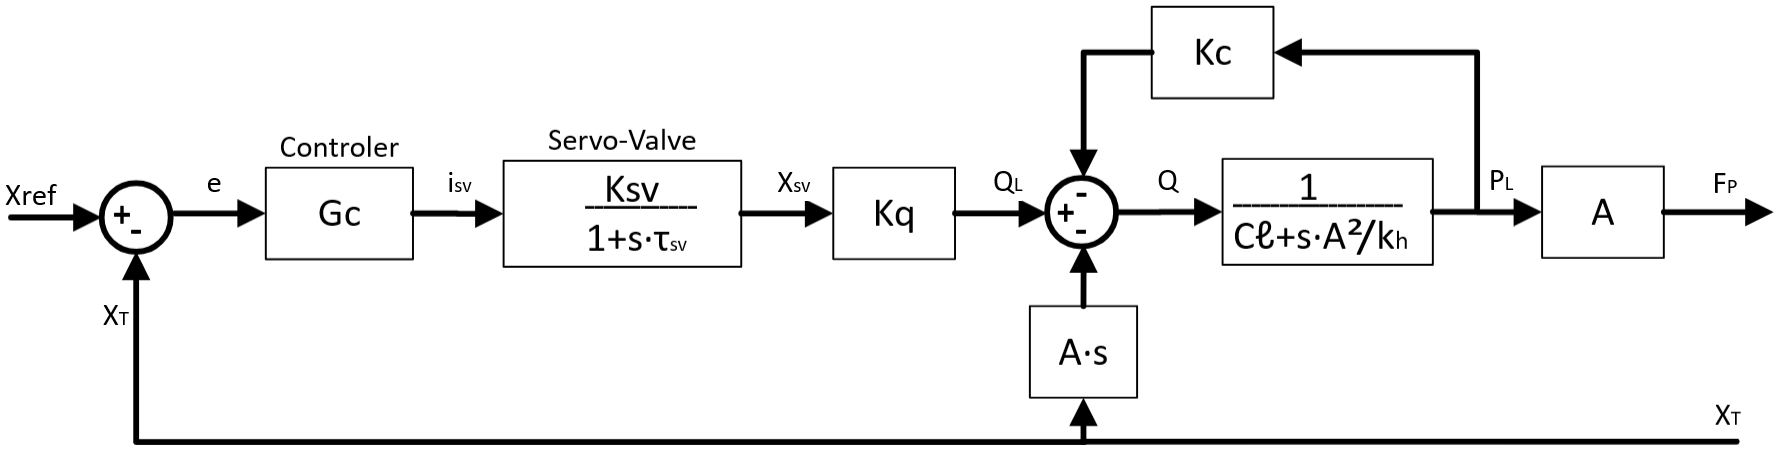
\includegraphics[width=0.8\linewidth]{Modelling/ST1D_block_diagram.png}
        % \begin{tikzpicture}[
        %     block/.style = {draw, thick, rectangle, minimum height=2.2em, align=center},
        %     sum/.style   = {draw, thick, circle, minimum size=2em, inner sep=0pt},
        %     >=Stealth, thick, font=\small,
        %     node distance=2.0cm and 1.6cm
        %     ]

        %     %--- Main signal path ---
        %     \node (xref) {$X_{\mathrm{ref}}$};

        %     \node[sum, right=2.0cm of xref] (s1) at (0,0) {};
        %     \node[font=\tiny] at ($(s1)+(-0.30, 0.25)$) {$+$};
        %     \node[font=\tiny] at ($(s1)+(-0.08,-0.33)$) {$-$};

        %     \node[block, minimum width=1.6cm, right=of s1, label=above:{\footnotesize Controler}] (gc) {$G_c$};

        %     \node[block, minimum width=3.6cm, right=of gc, label=above:{\footnotesize Servo-Valve}] (sv)
        %         {$\dfrac{K_{sv}}{1+s\cdot\tau_{sv}}$};

        %     \node[block, minimum width=1.6cm, right=of sv] (kq) {$K_q$};

        %     \node[sum, right=of kq] (s2) {};
        %     \node[font=\tiny] at ($(s2)+(-0.33, 0.25)$) {$+$};
        %     \node[font=\tiny] at ($(s2)+(-0.33,-0.25)$) {$-$};

        %     \node[block, minimum width=4.0cm, right=of s2] (hyd)
        %         {$\dfrac{1}{C_\ell + s\cdot A^2/k_h}$};

        %     \node[block, minimum width=1.6cm, right=of hyd] (Abl) {$A$};

        %     \node[right=of Abl] (fp) {$F_P$};

        %     %--- Feedback blocks ---
        %     \node[block, minimum width=1.6cm, above=3.2cm of hyd] (kc) {$K_c$};
        %     \node[block, minimum width=1.6cm, below=2.8cm of s2] (As) {$A\cdot s$};

        %     %--- Forward path arrows ---
        %     \draw[->] (xref) -- (s1);
        %     \draw[->] (s1)   -- node[above]{$e(t)$}        (gc);
        %     \draw[->] (gc)   -- node[above]{$i_{sv}$}   (sv);
        %     \draw[->] (sv)   -- node[above]{$x_{sv}$}   (kq);
        %     \draw[->] (kq)   -- node[above]{$Q_L$}      (s2);
        %     \draw[->] (s2)   -- node[above]{$Q$}        (hyd);
        %     \draw[->] (hyd)  -- node[above]{$P_L$}      (Abl);
        %     \draw[->] (Abl)  -- (fp);

        %     %--- Kc feedback path ---
        %     \coordinate (pl_tap) at ($(hyd.east)!0.5!(Abl.west)$);
        %     \draw (pl_tap) -- ++(0,3.2) coordinate (kc_in);
        %     \draw[->] (kc_in) -- (kc.east);
        %     \draw[->] (kc.west) -- ++(-1.5,0) |- (s2.north);

        %     %--- XT bottom feedback line ---
        %     \draw (s1.south) -- ++(0,-1.4) coordinate (xt_left);
        %     \draw (As.south) -- ++(0,-1.4) coordinate (xt_mid);
        %     \draw[->] (xt_left) -- ++(18.0,0) node[right]{$X_T$};
        %     \draw[->] (xt_left) -- (s1.south);   % into s1 (negative)
        %     \draw[->] (xt_mid)  -- (As.north);   % into A·s
        %     \draw[->] (As.north) -- (s2.south);  % A·s output into s2 (negative)

        % \end{tikzpicture}
    \caption{Block diagram of the ST1D}%, with position $X_{ref}$ as input and force applied to the platen $F_P$ as output.
    \label{fig_clean_block_force_output}
\end{figure}

 And the relevant transfer functions were derived:

% LTeX: enabled=false
\begin{align}
\left\{
    \begin{aligned}
        G_C(s) &= \frac{i_{sv}}{e} = \frac{i_{sv}}{x_{\text{ref}} - x_T} \\
        \frac{Q_L}{x_{\text{ref}} - x_T} &= \frac{Q_L}{e} = K_q \cdot \frac{K_{\text{sv}}}{1 + \tau_{\text{sv}} s} \cdot G_C(s) \\
    \end{aligned}
\right.
\Longrightarrow G_{csv}(s) &=  \frac{Q_L}{e} = \frac{k_{sv} k_q G_c}{1 + \tau_{sv} s} 
\end{align}

\begin{align}\label{eq_G_Fp_isv}
    \begin{aligned}
    & P_L = \frac{1}{C_l + \frac{A^2}{k_h}\cdot s} [Q_L - A \cdot s \cdot x_T - k_c \cdot P_L] \Longleftrightarrow \\
    & \Longleftrightarrow \frac{F_P}{i_{sv}} = \frac{A \cdot \frac{k_{sv} k_q}{1 + \tau_{sv} s} } {  k_{Pl} + \frac{A^2}{k_h}\cdot s  + A^2\cdot s \cdot G_{xT/Fp}} = G_{Fp/i_{sv}}(s) \quad \text{, where $k_{Pl}=k_c + C_l$}
    \end{aligned}
\end{align}
% LTeX: enabled=true
It's important to note that the transfer function $G_{Fp/i_{sv}}(s)$  is also a function of the model coupled to the platform (see Eq.\eqref{eq_G_Fp_isv} and  Eq.\eqref{G_xT_Fp}).

To represent the main dynamics of usual test specimens, a 2 degree of freedom mass-spring-damper system is coupled to the platen, as depicted in figure \ref{schematic_2dof}:

\begin{figure}[H]
\centering
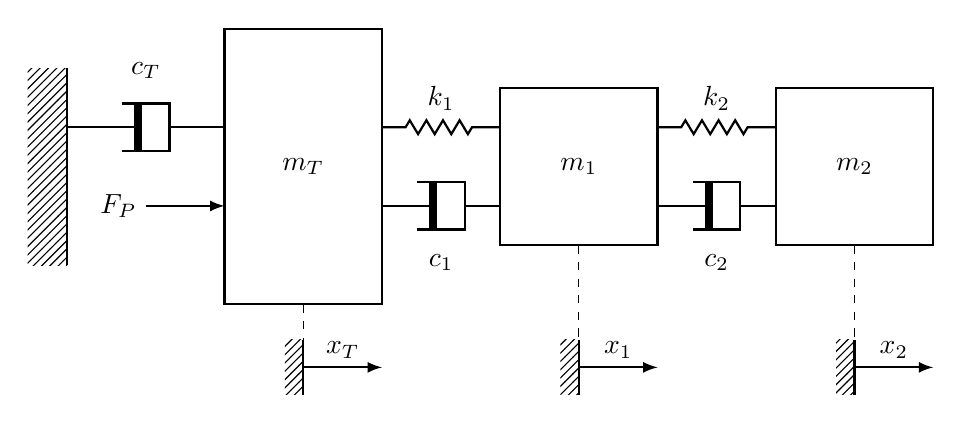
\begin{tikzpicture}[
    every node/.style={outer sep=0pt}, thick, % Set default node style and line thickness
    mass/.style={draw, thick}, % Define style for masses (rectangles)
    spring/.style={thick, decorate, decoration={zigzag, pre length=0.3cm, post length=0.3cm, segment length=6}}, % Define style for springs
    ground/.style={fill, pattern=north east lines, draw=none, minimum width=0.75cm, minimum height=0.3cm}, % Define style for ground
    dampic/.pic={ % Define a small pictogram for a damper
        \fill[white] (-0.1,-0.3) rectangle (0.3,0.3);
        \draw (-0.3,0.3) -| (0.3,-0.3) -- (-0.3,-0.3);
        \draw[line width=1mm] (-0.1,-0.3) -- (-0.1,0.3);
    }
]

    % Define the mass blocks
    \node[mass, minimum width=2cm, minimum height=3.5cm] (mT) {$m_T$}; % First mass 
    \node[mass, minimum width=2cm, minimum height=2cm, right=1.5cm of mT] (m1) {$m_1$}; % Second mass
    \node[mass, minimum width=2cm, minimum height=2cm, right=1.5cm of m1] (m2) {$m_2$}; % Third mass

    % Define the ground (left of mT)
    \node[left=2cm of mT, ground, minimum width=5mm, minimum height=25mm ] (ground) {}; 
    \draw (ground.north east) -- (ground.south east); % Draw vertical edge of the ground block

    % Connect the ground to mT with a damper
    \draw ([yshift=5mm]ground.east) coordinate(aux) -- (mT.west|-aux) 
        pic[midway]{dampic} node[midway, above=5mm]{$c_T$}; % Damper from ground to mT

    % Draw springs between elements
    \draw[spring] (mT.east|-aux) -- (m1.west|-aux) node[midway, above=1mm]{$k_1$}; % Spring from mT to m1
    \draw[spring] (m1.east|-aux) -- (m2.west|-aux) node[midway, above=1mm]{$k_2$}; % Spring from m1 to m2

    % Draw dampers in parallel with the springs
    \draw ([yshift=-5mm]mT.east) coordinate(aux') -- (m1.west|-aux') 
        pic[midway]{dampic} node[midway, below=5mm]{$c_1$}; % Damper from mT to m1
    \draw (m1.east|-aux') -- (m2.west|-aux') 
        pic[midway]{dampic} node[midway, below=5mm]{$c_2$}; % Damper from m1 to m2

    % Define a common baseline for displacement markers
    \coordinate (disp_line) at ([yshift=-8mm]mT.south);
    % Draw displacement markers inline using common baseline
    \foreach \X in {T,1,2} {  
        \draw[thin, dashed] (m\X.south) -- (m\X.south |- disp_line); % Align displacement lines
        \draw[latex-] (m\X.east |- disp_line) -- ++ (-1,0) node[midway, above]{$x_\X$} % Labels for x_T, x_1, x_2
            node[left, ground, minimum height=7mm, minimum width=1mm] (g'\X){};
        \draw[thick] (g'\X.north east) -- (g'\X.south east); 
    }

    % Draw force input on mT
    \draw[latex-] ([yshift=-5mm]mT.west) -- ++ (-1,0) node[left]{$F_P$}; % Force applied to mT
\end{tikzpicture}
\caption{Schematic representation of the 2 degree of freedom mass-spring-damper system coupled to the platen}
\label{schematic_2dof}
\end{figure}


%\vspace{5mm}
For the system in figure \ref{schematic_2dof} the following equations of motion are obtained (system of equations \eqref{eq_2dof_system}):

\begin{align}\label{eq_2dof_system}
\left\{
\begin{aligned}
    m_T \cdot \ddot{x}_T &+ c_T \cdot \dot{x}_T + c_1 (\dot{x}_T -  \dot{x}_1) + k_1 (x_T - x_1) = F_p \\
    m_1 \cdot \ddot{x}_1 &+ c_1 ( \dot{x}_1 -\dot{x}_T) + c_2 ( \dot{x}_1 - \dot{x}_2) + k_1 (x_1 - x_T) + k_2 (x_1 - x_2) = 0 \\
    m_2 \cdot \ddot{x}_2 &+ c_2 ( \dot{x}_2 -\dot{x}_1) + k_2 (x_2 - x_1) = 0
\end{aligned}
\right. 
\Longleftrightarrow
\end{align}

%\vspace{5mm}

\begin{equation*} 
\Longleftrightarrow
\left\{
\begin{aligned}
    &m_T  \ddot{x}_T + (c_T + c_1)  \dot{x}_T + k_1 x_T - c_1  \dot{x}_1 - k_1  x_1 = F_p \\
    &m_1  \ddot{x}_1 + (c_1 + c_2) \dot{x}_1 + (k_1 + k_2) x_1 - c_1  \dot{x}_T - c_2  \dot{x}_2 - k_1  x_T - k_2 x_2 = 0 \\
    &m_2  \ddot{x}_2 + c_2 \dot{x}_2 + k_2 x_2 - c_2  \dot{x}_1 - k_2 x_1 = 0
\end{aligned}
\right.
\Longleftrightarrow
\end{equation*}

%\vspace{5mm}

\begin{equation*}
\Longleftrightarrow
\begin{bmatrix}
    m_T & 0 & 0 \\
    0 & m_1 & 0 \\
    0 & 0 & m_2
\end{bmatrix}
\begin{bmatrix}
    \ddot{x}_T \\ \ddot{x}_1 \\ \ddot{x}_2
\end{bmatrix}
+
\begin{bmatrix}
    c_T + c_1 & -c_1 & 0 \\
    -c_1 & c_1 + c_2 & -c_2 \\
    0 & -c_2 & c_2
\end{bmatrix}
\begin{bmatrix}
    \dot{x}_T \\ \dot{x}_1 \\ \dot{x}_2
\end{bmatrix}
+
\begin{bmatrix}
    k_1 & -k_1 & 0 \\
    -k_1 & k_1 + k_2 & -k_2 \\
    0 & -k_2 & k_2
\end{bmatrix}
\begin{bmatrix}
    x_T \\ x_1 \\ x_2
\end{bmatrix}
=
\begin{bmatrix}
    F_p \\ 0 \\ 0
\end{bmatrix}
\end{equation*}
  
%\vspace{5mm}
From the system of equations \eqref{eq_2dof_system}, the following transfer functions relating the displacements of each mass to the displacements of an adjacent mass, or the force applied to the platen, are obtained:

\begin{align}
    \frac{x_T}{F_P} &= \frac{G_1 G_2 - G_{21}^2}{G_T G_1 G_2 - G_T G_{21}^2 - G_2 G_{T1}^2} = G_{xT/Fp}(s) \label{G_xT_Fp}\\
    \frac{x_1}{x_T} &= \frac{G_{T1} G_2}{G_1 G_2 - G_{21}^2} = G_{x1/xT}(s) \\
    \frac{x_2}{x_1} &= \frac{G_{21}}{G_2} = G_{x2/x1}(s)\\
    G_T(s) &= m_T\cdot s^2 + (c_T + c_1)\cdot s + k_1 \\
    G_1(s) &= m_1\cdot s^2 + (c_1 + c_2)\cdot s + k_1 + k_2 \\
    G_2(s) &= m_2\cdot s^2 + c_2\cdot s + k_2 \\
    G_{T1}(s) &= c_1\cdot s + k_1 \\
    G_{21}(s) &= c_2\cdot s + k_2 \\
    G_{Fp/x_{ref}}(s) &= \frac{G_{csv}}{\frac{k_{pl}}{A} + \frac{A}{k_h} s + G_{xT/Fp} (G_{csv} + A\cdot s)} \\
    G_{xT/x_{ref}}(s) &= G_{Fp/x_{ref}} \cdot G_{xT/Fp} 
    %\\
    % G_{x1/x_{ref}}(s) &= G_{x1/xT} \cdot G_{xT/x_{ref}} \\
    % G_{x2/xT}(s) &= G_{x2/x1} \cdot G_{x1/xT}
\end{align}

The mass $m_i$, stiffness $k_i$, and damping $c_i$, of each element will be determined such that the system's natural frequencies $f_i$ and damping ratios $\xi_i$ are similar to the structures in test. Equation \eqref{eq_modal_frequencies} relates the natural frequency of the two modes of the 2DoF system to it's spring and mass properties, and equation \eqref{eq_modal_damping} relates the damping coefficient and ratio to mass and natural frequency.

\begin{equation}\label{eq_modal_frequencies}
\omega_{1,2}^{2} = \frac{1}{2}\frac{m_1 k_2 + m_2 (k_1 + k_2)}{m_1 m_2} \mp \frac{1}{2} \sqrt{\left( \frac{m_1 k_2 + m_2 (k_1 + k_2)}{m_1 m_2} \right)^2 - 4 \frac{k_1 k_2}{m_1 m_2}} 
\end{equation}

\begin{equation}\label{eq_modal_damping} 
    \xi_i = \frac{ c_i}{2\cdot m_i\cdot \omega_i}
\end{equation}

%\clearpage
\section{Control Strategies}

In this section two new control strategies are proposed: a tuned PID-F controller, and an optimal controller. This control strategies are then evaluated against LNEC's iterative driver adaptation method, which is currently used.

In sections \ref{sec_Tuned_PID-F} and \ref{sec_Optimal_Control}, for a preliminary analysis of how the shaking table performance could be affected by controller tuning, simulations were run using the seismic data from the 1979  Imperial Valley Earthquake, El Centro (Described in \cite{narasimhan2006}), fault normal direction, which was scaled down to $73.51\%$, in order to comply with the displacement range of the shaking table ($\pm 100mm$).

It was also considered throughout that the platen had a 2DOF coupled structure, as in figure \ref{schematic_2dof}, and the parameters of this 2DOF system, unless stated otherwise, are the ones shown in table \ref{tab:modal_params}:

\begin{table}[H]
    \centering
    \caption{Modal parameters for the system, and resulting stiffness and damping for each element}
    \renewcommand{\arraystretch}{1.3}
    \begin{tabular}{ c c c }
        \hline
        \textbf{System Properties} & \textbf{1st Mode} & \textbf{2nd Mode} \\
        \hline
        Frequency ($f_i$) [Hz] & $4$ & $10$ \\
        %\hline
        Damping Ratio ($\zeta_i$) & $0.02$ & $0.05$ \\
        \hline
        \textbf{Element's Properties} & \textbf{Element 1} & \textbf{Element 2} \\
        \hline
        Mass ($m_i$) [kg] & $2000$ & $2000$ \\
        %\hline
        Stiffness ($k_i$) [N/m] & $3.30\cdot 10^5$ & $1.89\cdot 10^6$ \\
        %\hline
        Damping Coefficient ($c_i$) [N$\cdot$m/s] & $1.26\cdot 10^3$ & $1.26\cdot 10^4$ \\
        \hline
    \end{tabular}
    \label{tab:modal_params}
\end{table}

In section \ref{sec_LNEC_method}, LNEC's control strategy is entirely explained, while showing the working of the software used in the iterative driver adaptation method. An application example is shown, and the method and results are discussed.

In section \ref{sec_Comparing_Control_Strategies}, the performance of the three control strategies is compared for a set of benchmark seismic signals.
 
\subsection{Tuned PID-F} \label{sec_Tuned_PID-F}

Taking into consideration the test procedure at LNEC (figure \ref{fig_lnec_test_process_diagram}), where the identification is carried out each time the target signal is scaled up, or even additional times for various other reasons, one possible straightforward improvement would be to update the PI controller tune using this information, as in an adaptive control strategy (figure \ref{fig_adaptive_diagram}).

% \begin{figure}[H]
% \noindent
% \begin{minipage}{0.49\textwidth}\setlength{\parindent}{15pt}
    Another simple enhancement would be to add a filtered derivative term to the controller (making it a PID-F), since this would allow more tuning flexibility, should improve the tracking for the typical fast changing seismic displacement reference signal, and be of simple implementation in the existing version of the control software due to the fact that it's just an extension of the existing controller structure. 
% \end{minipage}
% \hfill
% \begin{minipage}{0.49\textwidth}
\begin{figure}[H]
\centering
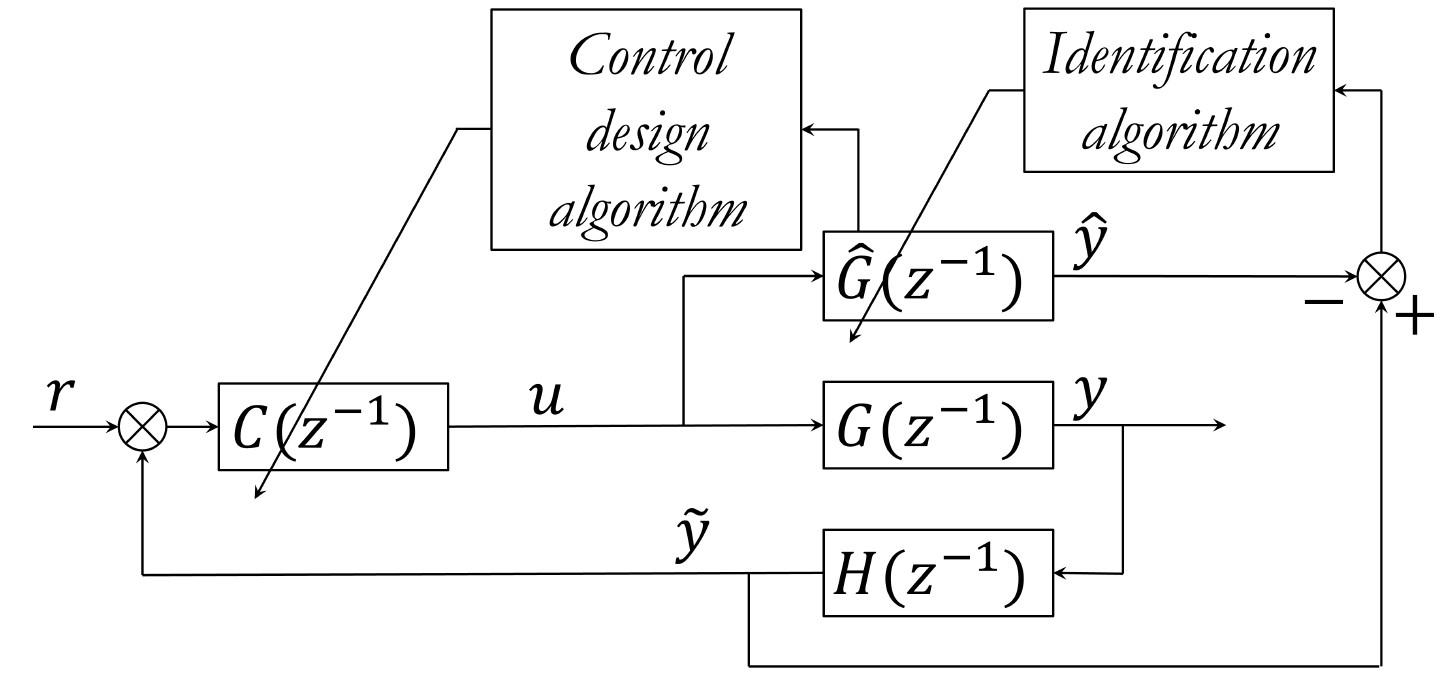
\includegraphics[width=0.5\linewidth]{adaptive_diagram.jpg} %0.5
\caption{Adaptive control scheme \citep{DuarteValerio}}
\label{fig_adaptive_diagram}
\end{figure}
% \end{minipage}


Initially the simulations were run with the controller set as $G_c(s)=129.93$ V/m, as in \cite{tekeste2021}. Afterwards, a simulation was run with controller in the form of a PID-F : $G_c(s) = K_p +  \frac{K_i}{s} +  \frac{K_d\cdot s}{T_f\cdot s + 1}$ ,
% \begin{equation} \label{eq_pidf_in_s}
%     G_c(s) = K_p +  \frac{K_i}{s} +  \frac{K_d\cdot s}{T_f\cdot s + 1}
% \end{equation}
where the parameters $K_p, K_i, K_d$, and $T_f$, seen in table \ref{tab:pidf_params}, were computed using MATLAB's \textit{pidtune} function, with the tuning option \textit{'DesignFocus'} set to \textit{'reference-tracking'}. These results are labelled as "tuned" in figures \ref{fig_response_spectrum_of_3} through to \ref{fig_Platen_Displacement_Tracking_Error}. The code implementation can be found at the following GitHub repository \href{https://github.com/c-radicallis/Controlo_Plataforma_Sismica/blob/main/uniaxial_table_model/simulation_and_plotting.m}{location}.

\begin{table}[H]
    \centering
\begin{minipage}{0.48\textwidth} %0.37
        \centering
    \caption{Tuned PID-F controller parameters}
    \begin{tabular}{ccc}
        \hline
        Parameter & Value & Units \\
        \hline
        $K_p$ & $1540$ & $V/m$ \\
        $K_i$ & $1670$ & $V/(m \, s)$ \\
        $K_d$ & $17.9$ & $V/(m/s)$ \\
        $T_f$ & $6.96\cdot10^{-5}$ & $s$ \\
        \hline
    \end{tabular}
    \label{tab:pidf_params}
\end{minipage}
\hspace{5mm}
\begin{minipage}{0.46\textwidth} 
    \centering
    \caption{Mean squared error for response spectra of platen, with the seismic signal ground response spectra as target.}
    \label{tab:mse_rs}
    \begin{tabular}{ccc}
        \hline
        Controller & Acceleration  & Displacement \\[-2mm]
                   & MSE ($m/s^2$) & MSE ($m$)    \\
        \hline
        Baseline & $1.78$               & $1.94 \cdot 10^{-6}$ \\
        Tuned    & $3.27 \cdot 10^{-2}$ & $1.88 \cdot 10^{-6}$ \\
        \hline
    \end{tabular}
\end{minipage}
\end{table}

%\pagebreak

The mean squared error (MSE) of the platen response spectrum,  having the ground response spectrum as target, was used as a metric to evaluate the performance of the shaking table. The comparison was performed in terms of displacement and acceleration response spectrum, which was computed for 500 logarithmically spaced frequencies between 0.1 and 30 Hz (figure \ref{fig_response_spectrum_of_3}).

The acceleration response spectrum mean squared error for the tuned platform is significantly reduced compared to the standard tune (Table \ref{tab:mse_rs}), however, it exceeds the desired response spectrum for the entire frequency spectrum (figure \ref{fig_response_spectrum_of_3}).

% \begin{table}[H]
%     \centering
%     \caption{Mean squared error for response spectra of platen, with the seismic signal ground response spectra as target.}
%     \label{tab:mse_rs}
%     \begin{tabular}{ c c c }
%         \hline
%         Controller & Acceleration MSE ($m/s^2$) & Displacement MSE ($m$) \\
%         \hline
%         Baseline & $1.78$               & $1.94 \cdot 10^{-6}$ \\
%         Tuned    & $3.27 \cdot 10^{-2}$ & $1.88 \cdot 10^{-6}$ \\
%         \hline
%     \end{tabular}
% \end{table}

In figures \ref{fig_Platen_Acceleration} to \ref{fig_Platen_Displacement_zoom}, label "MSE" refers to the  respective mean squared error when using the standard controller, and "Tuned MSE" refers to the respective mean squared error when using the tuned PID-F controller. All values are presented in SI units, in this case, $m/s^2$ for the acceleration response spectrum MSE, and $m$ for the displacement response spectrum MSE.

The detailed view in figures \ref{fig_Platen_Acceleration_zoom} and \ref{fig_Platen_Displacement_zoom} highlights the faster response of the tuned controller, and its improved tracking. It also highlights how the tuned controller now introduces some overshoot, which is also apparent in the response spectra of figure \ref{fig_response_spectrum_of_3}, and the bode plot in figure \ref{fig_Bode_of_G_xT_xref}.


\begin{figure}[H]
    \centering
    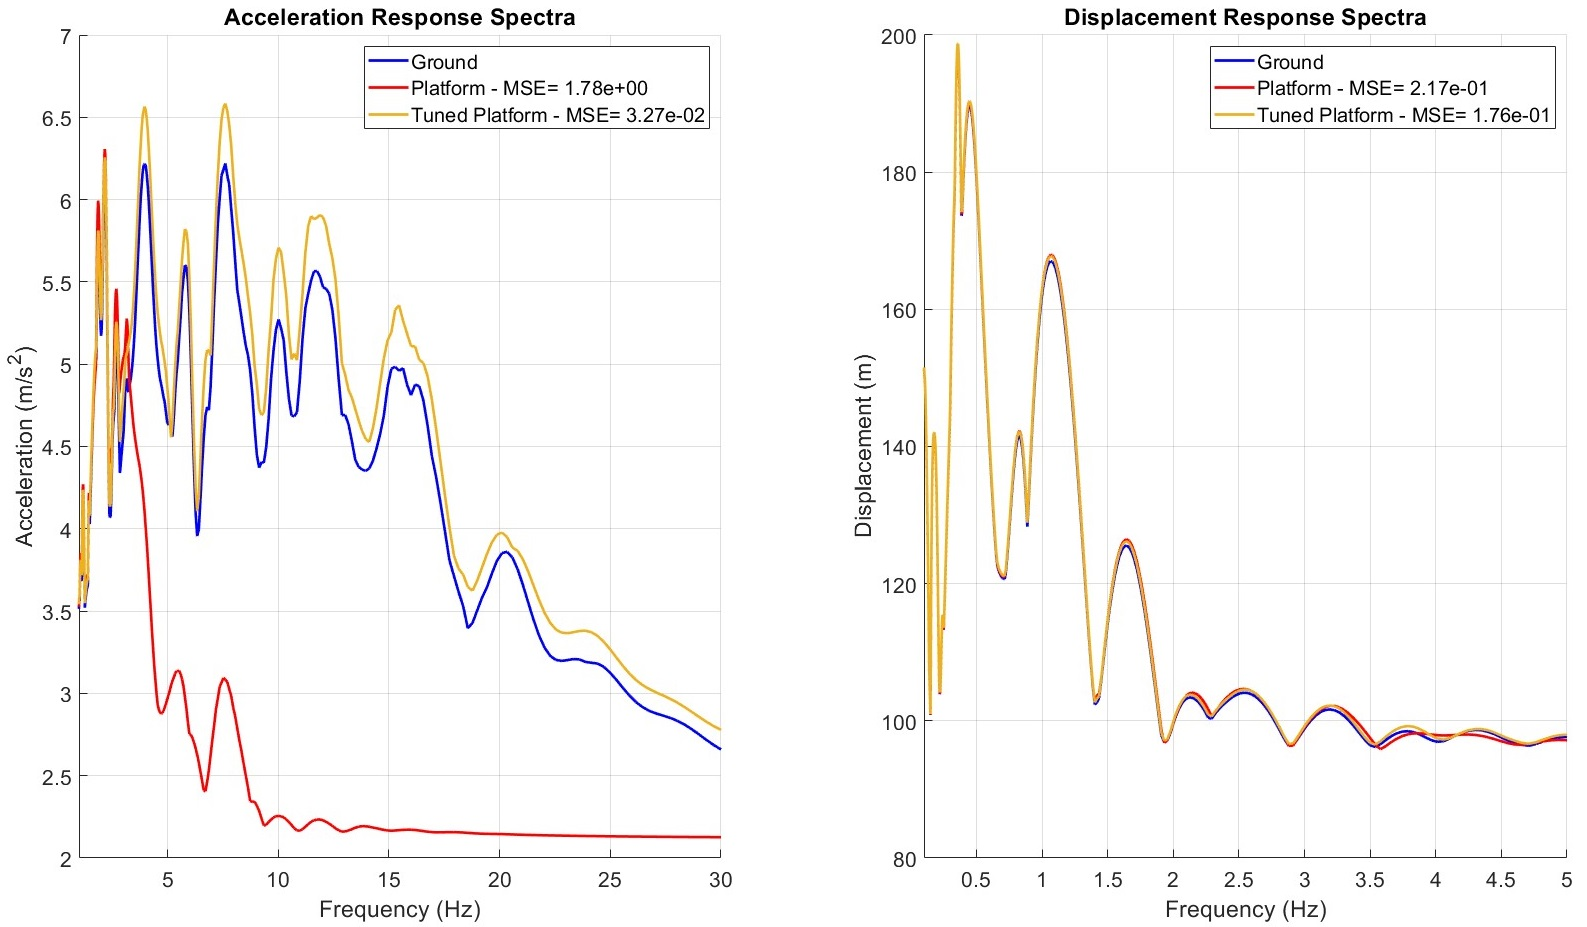
\includegraphics[width=\linewidth]{Sim_Res/Response_Spectra.jpg}
    \caption{Response spectra for fault normal signals. The response spectrum was obtained by sampling 500 frequencies, logarithmically spaced between 0.1 and 30 Hz.}
    \label{fig_response_spectrum_of_3}
\end{figure}

\begin{figure}[H]
\begin{minipage}{0.49\textwidth}
    \centering
    
\includegraphics[width=\linewidth]{Sim_Res/Bode_of_G_xT_xref.png}
    \caption{Bode plots of $G_{xT/x_{\text{ref}}}(s)$ before and after tuning}
    \label{fig_Bode_of_G_xT_xref}    
\end{minipage}
\hfill
\begin{minipage}{0.49\textwidth}
    \centering
    
\includegraphics[width=\linewidth]{Sim_Res/Input_to_Servo.png}
    \caption{Input to servo before and after tuning}
    \label{fig_Input_to_Servo}
\end{minipage}
\end{figure}


\begin{figure}[H]
\begin{minipage}{0.49\textwidth}
    \centering
    
\includegraphics[width=\linewidth]{Sim_Res/Platen_Acceleration.png}
    \caption{Platen acceleration before and after tuning}
    \label{fig_Platen_Acceleration}
\end{minipage}
\hfill
\begin{minipage}{0.49\textwidth}
    \centering
    
\includegraphics[width=\linewidth]{Sim_Res/Platen_Displacement.png}
    \caption{Platen displacements before and after tuning}
    \label{fig_Platen_Displacement}
\end{minipage}
\end{figure}

\begin{figure}[H]
\begin{minipage}{0.49\textwidth}
    \centering
    
\includegraphics[width=\linewidth]{Sim_Res/Platen_Acceleration_zoom.png}
    \caption{Platen acceleration before and after tuning - Detailed view of the signals covering the period between 1.5 and 2.7 seconds}
    \label{fig_Platen_Acceleration_zoom}
\end{minipage}
\hfill
\begin{minipage}{0.49\textwidth}
    \centering
    
\includegraphics[width=\linewidth]{Sim_Res/Platen_Displacement_zoom.png}
    \caption{Platen displacements before and after tuning - Detailed view of the signals covering the period between 14.1 and 15.7 seconds}
    \label{fig_Platen_Displacement_zoom}
\end{minipage}
\end{figure}

\begin{figure}[H]
\begin{minipage}{0.49\textwidth}
    \centering
    
\includegraphics[width=\linewidth]{Sim_Res/Platen_Acceleration_Tracking_Error.png}
    \caption{Acceleration tracking error before and after tuning}
    \label{fig_Platen_Acceleration_Tracking_Error}
\end{minipage}
\hfill
\begin{minipage}{0.49\textwidth}
    \centering
    
\includegraphics[width=\linewidth]{Sim_Res/Platen_Displacement_Tracking_Error.png}
    \caption{Displacement tracking error before and after tuning}
    \label{fig_Platen_Displacement_Tracking_Error}
\end{minipage}
\end{figure}

\subsubsection{Tuned PID-F Performance Sensitivity to Test Specimen Parameters} \label{Tuned PID-F Performance Sensitivity}%Analysis of Tuned PID-F 

The mass, modal frequencies, and damping of the specimens coupled to the shaking table have an impact on how well it is able to track the reference. In this section, we will analyse how the shaking table performs for different damping, modal frequencies, and mass of the test specimen with the tuned PID-F controller (which is tuned for each case).

Specimens with % higher modal frequencies ($f_1=4$ Hz \& $f_2=10$ Hz) and 
lower damping ($\zeta_1=0.02$ \& $\zeta_2=0.05$) result in response spectra which exceeds the desired one over the entire frequency spectrum, while structures with higher damping ($\zeta_1=0.1$ \& $\zeta_2=0.25$) result in response spectra which fall short of the desired one (figures \ref{Resp_Spectre_low_high_freq_and_damp} through to \ref{Resp_Spectre_f1_2415}), and this translates to trend observed in figure \ref{fig_MSE_vs_damping}.

\begin{figure}[H]
\centering
    \begin{subfigure}{0.64\textwidth}
        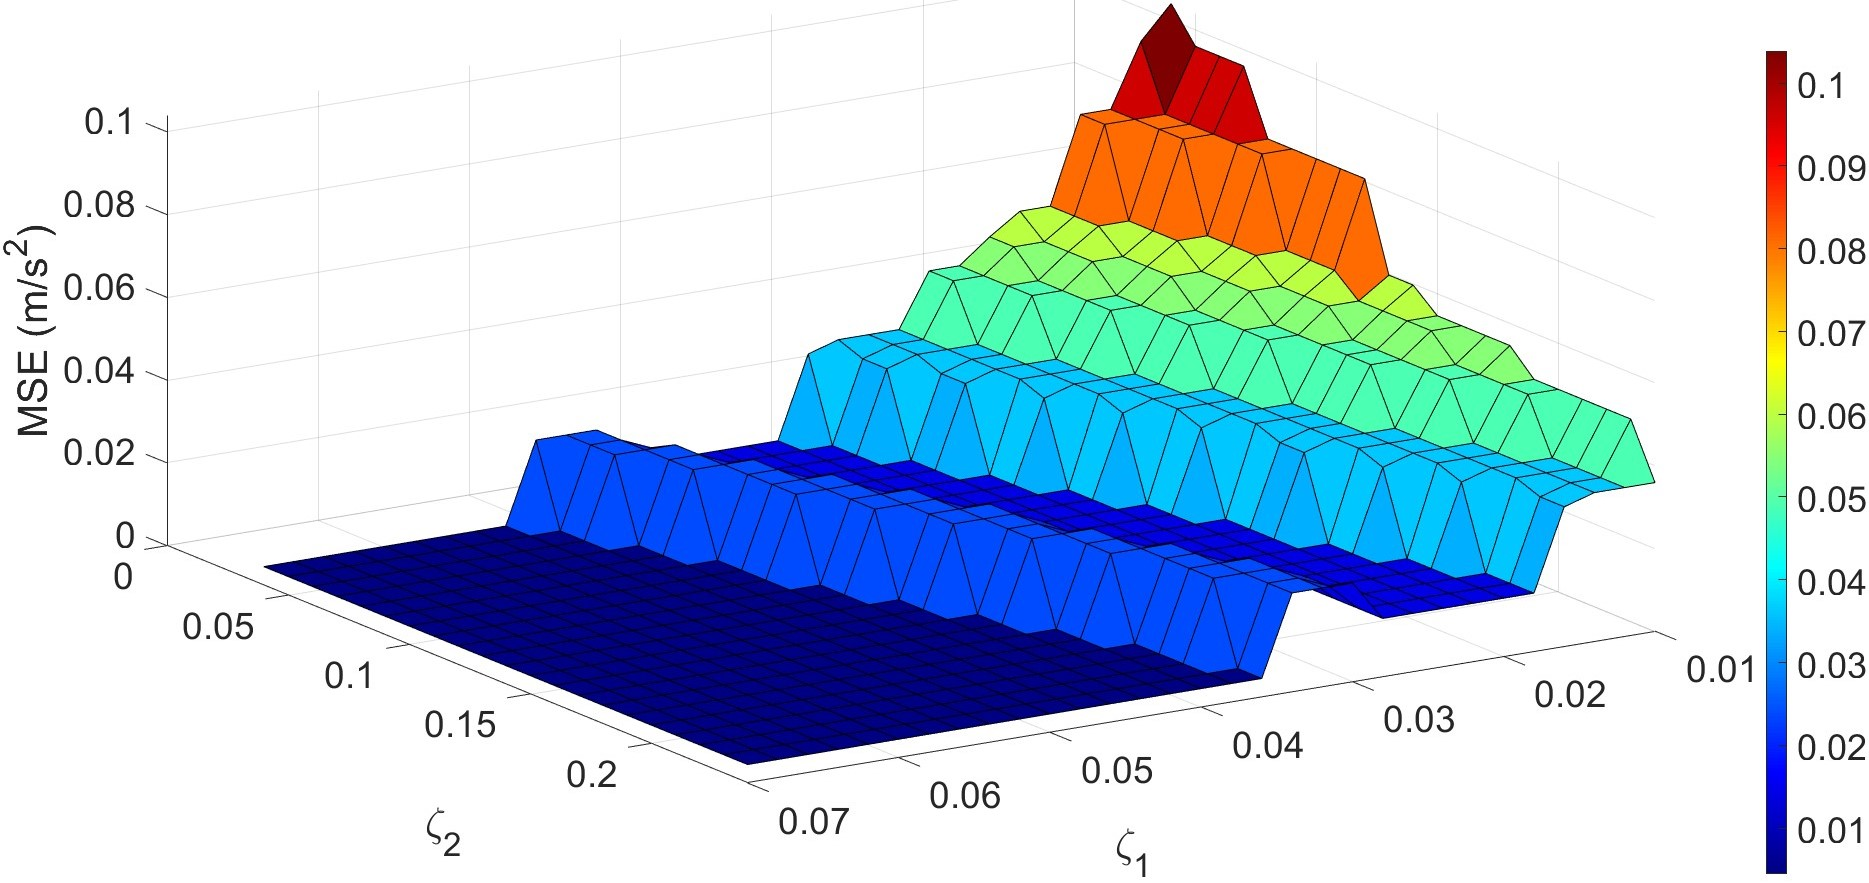
\includegraphics[width=\textwidth]{MSE_Zeta/Surf_Zeta_LowFreq_iso_cut.jpg}
        \caption{Isometric view}
        \label{fig:first}
    \end{subfigure}
    \hfill
    \begin{subfigure}{0.35\textwidth}
        \centering
        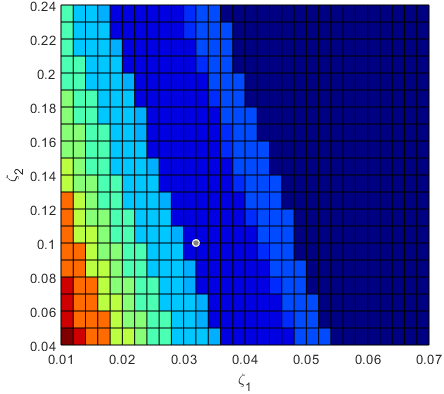
\includegraphics[width=\textwidth]{MSE_Zeta/Surf_Zeta_LowFreq_TopView_cut.png}
        \caption{Top view}
        \label{fig:second}
    \end{subfigure}
\caption{Acceleration response spectra MSE ($m/s^2$) vs damping ($\zeta_1$ and $\zeta_2$), with $m_1=m_2=2\text{ ton, }f_1=1.5 Hz, f_2=6 Hz$}
\label{fig_MSE_vs_damping}
\end{figure}

The effect of modal frequencies on the performance of the shaking table (shown in figure \ref{fig_MSE_vs_modal_freqs}) is unclear in this analysis , most likely because the analysis was performed for a single seismic signal, and it depends heavily on the specific combination of frequency content of the seismic signal, and the closed-loop response of the system. It is expected that seismic signals with more power in frequencies close to the modal frequencies will result in an over-shoot of the target response spectra (especially if damping is low), if the closed-loop gain is close to unitary in that range, but if none of these conditions are met, for example, when the modal frequencies of the specimen are mismatched with the frequency content of the seismic signal, or they are beyond the bandwidth of the closed-loop, than it is expected that the response spectra will closely match the target, or, in the second case, undershoot.

\begin{figure}[H]
    \centering
    \begin{subfigure}{\textwidth}
        \centering
        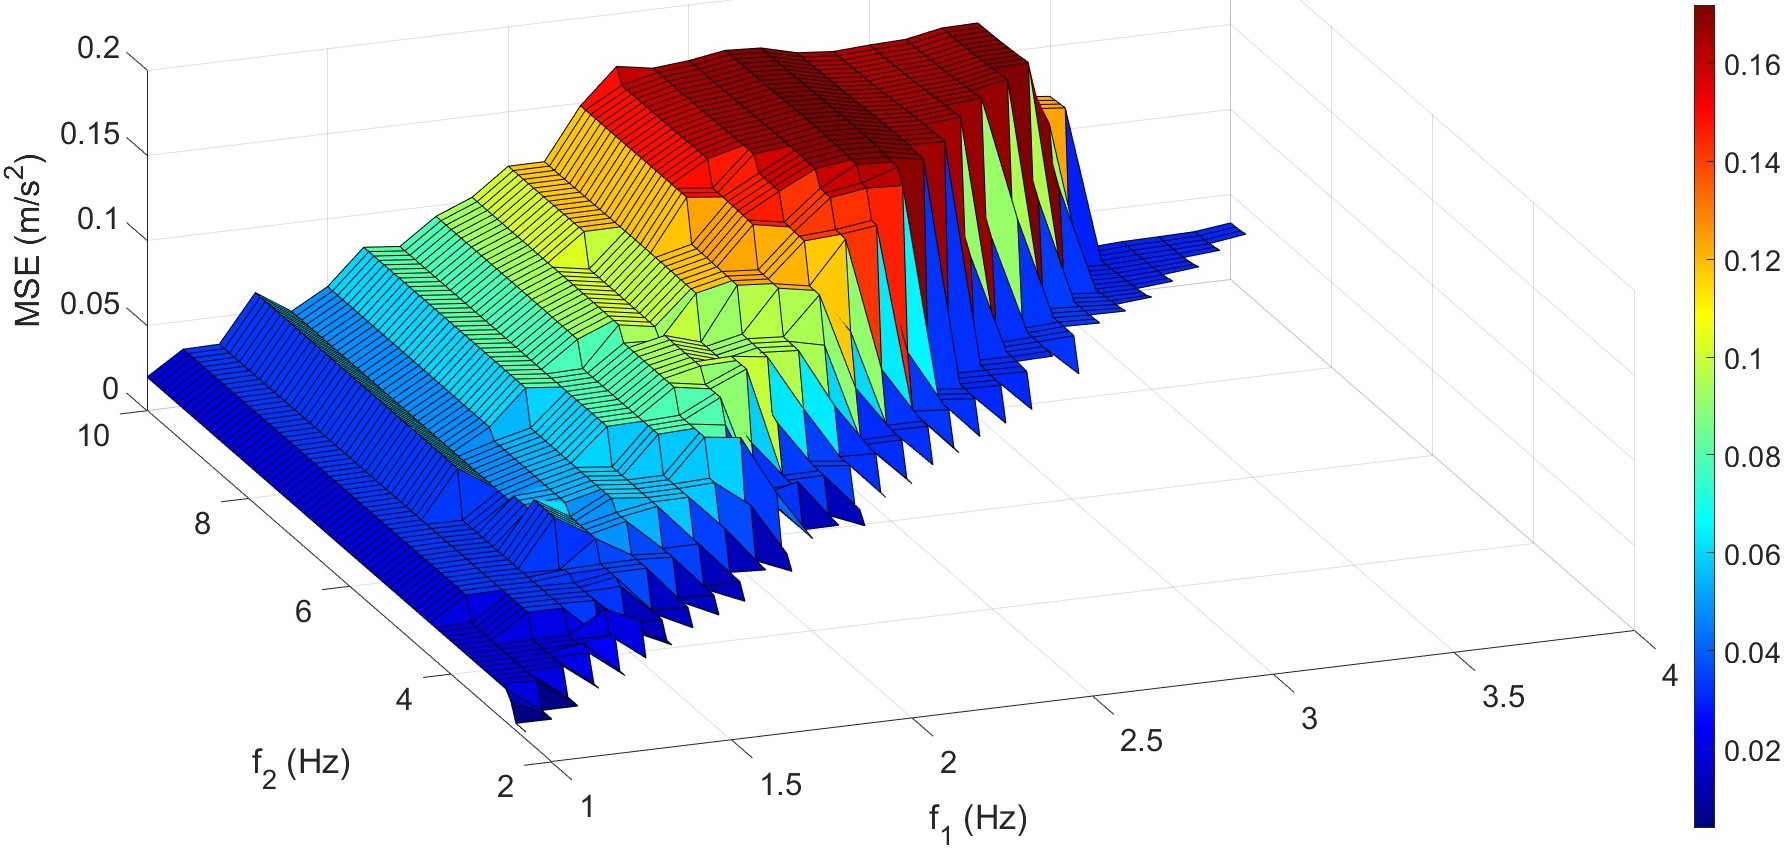
\includegraphics[width=1\linewidth]{PID_MSE/PID_MSE_Surface_frequency_lowDamp_iso_cut.jpg}
        \caption{Low damping: $\zeta_1=0.02, \zeta_2=0.05$ }
        %\label{}
    \end{subfigure}
    \\
    \begin{subfigure}{0.49\textwidth}
        \centering
        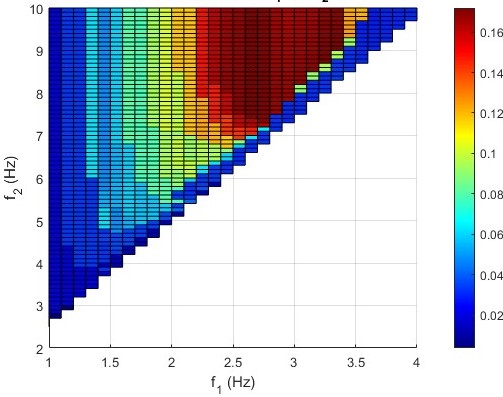
\includegraphics[width=1\linewidth]{PID_MSE/PID_MSE_Surface_frequency_lowDamp_cut.jpg}
        \caption{Low damping: $\zeta_1=0.02, \zeta_2=0.05$ }
        %\label{}
    \end{subfigure}
    \hfill
    \begin{subfigure}{0.49\textwidth}
        \centering
        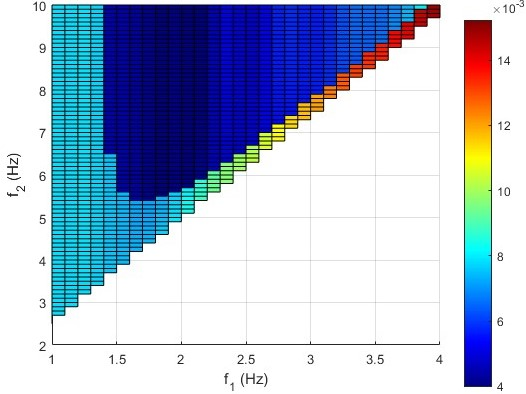
\includegraphics[width=1\linewidth]{PID_MSE/PID_MSE_Surface_frequency_highDamp_top.jpg}
        \caption{High damping: $\zeta_1=0.1, \zeta_2=0.25$ }
        %\label{}
\end{subfigure}
\caption{Acceleration response spectra MSE vs modal frequencies ($f_1$ and $f_2$), with $m_1=m_2=2\text{ ton }$}
\label{fig_MSE_vs_modal_freqs}
\end{figure}

In figures \ref{Resp_Spectre_low_high_freq_and_damp} through to \ref{Resp_Spectre_f1_2415} the response spectra are shown, and the same trends are observed. The legend shows the modal properties of the specimen under analysis, the maximum absolute values of the input to the servo-valve $i_{sv}$ (in volts) and force applied by the actuator (in kilo newtons), and the mean square error for the respective response spectrum (in their respective SI units).

In figure \ref{fig_close_modal_freqs}, where the modal frequencies are as tightly spaced as possible, for the acceleration spectra MSE a trend reversal is observed, where for $\zeta_2 \approx 0.1$ the MSE is lowest, and then increases for both lower and higher damping. This consistent with what is observed in figures \ref{Resp_Spectre_low_high_freq_and_damp} through to \ref{Resp_Spectre_f1_2415}, as it results from under-shooting and over-shooting the target response spectra from low and high damping, respectively.

For the high modal frequencies in figure \ref{fig_high_modal_freqs}, the response spectrum MSE increases abruptly for $\zeta_2 < 0.14 - 0.8\cdot \zeta_1 $, but remains mostly unchanged inside the two regions separated by that line. This shows that tiny differences in the damping of the specimen can translate to significant differences in the response spectra.

\begin{figure}[H]
\centering
    \begin{subfigure}{0.46\textwidth}
        \centering
        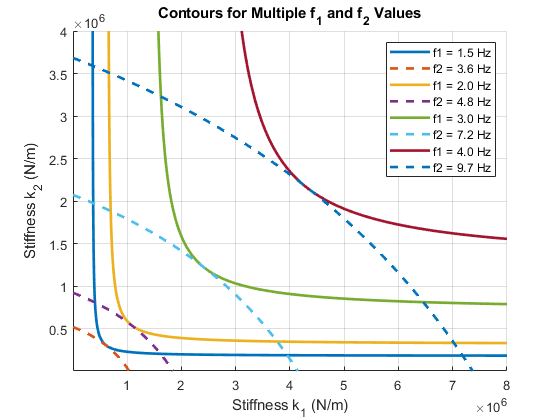
\includegraphics[width=\linewidth]{PID_MSE/stiffness_solutions.png}
        \caption{For the 2DOF model (fig. \ref{schematic_2dof}), the modal frequency $f_2$ must be greater than $2.415 \times f_1$  (Equation \eqref{eq_modal_frequencies})}
        \label{fig_k_for_close_modal_freqs}
    \end{subfigure}
    \hfill
    \begin{subfigure}{0.52\textwidth}
        \centering
        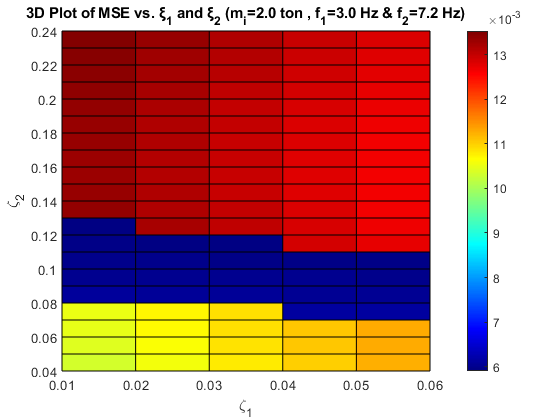
\includegraphics[width=1\linewidth]{MSE_Zeta/MSE vs Zeta (m_i=2.0,f_1=3.0, f_2=7.2).png}
        \caption{Acceleration response spectra MSE $(m/s^2)$ vs damping ($\zeta_1$ and $\zeta_2$), with $m_1=m_2=2\text{ ton, }f_1=3 Hz, f_2=7.2 Hz$}
        %\label{fig:enter-label}
    \end{subfigure}
\caption{Analysis for modal frequencies which are close together}
\label{fig_close_modal_freqs}
\end{figure}



%\clearpage
\subsection{Optimal Control}  \label{sec_Optimal_Control}

\subsubsection{ State Space Model} \label{section_ss_model}
For the shaking table with a coupled 2-DoF system, the following state space model representation was adopted:
\begin{align}
\dot{x}(t)  &=  A \cdot x(t) + B \cdot u(t) \\
y(t) &= C\cdot x(t) + D\cdot u(t)
\end{align}
With $x(t)$ being the state vector:
\begin{equation}
x = [Q_{sv} ,\, F_p ,\, x_T ,\, x_1 ,\, x_2 ,\, \dot{x}_T ,\, \dot{x}_1 ,\, \dot{x}_2 ]^{T}
\end{equation}
And the control action $u(t)$ (which is the signal to the servo-valve $i_{sv}$), the state equations are:
\begin{align}
    \begin{bmatrix} 
        \dot{Q}_{sv} \\[6pt]
        \dot{F}_p \\[6pt]
        \dot{x}_T \\[6pt]
        \dot{x}_1 \\[6pt]
        \dot{x}_2 \\[6pt]
        \ddot{x}_T \\[6pt]
        \ddot{x}_1 \\[6pt]
        \ddot{x}_2 
    \end{bmatrix} &=
    \begin{bmatrix}
    \frac{-1}{\tau_{sv}} &  0 & 0 & 0 & 0 & 0 & 0 & 0 & 0\\[6pt]
    \frac{k_h}{A}  & \frac{- k_h k_{pl}}{A^2} & 0              & 0 & 0                & 0   & -k_h & 0               & 0 \\[6pt]
                    0 &               0              & 0 & 0                & 0   & 1    & 0               & 0 \\[6pt]
                    0 &               0              & 0 & 0                & 0   & 0    & 1               & 0 \\[6pt]
                    0 &               0              & 0 & 0                & 0   & 0    & 0               & 1 \\[6pt]
                    0 &                \frac{1}{m_T} & \frac{-k_1}{m_T} & \frac{k_1}{m_T}     &  0              & \frac{-c_T - c_1 }{m_T} & \frac{ c_1 }{m_T}   & 0               \\[6pt]
                    0 &                0             & \frac{k_1}{m_1}  &\frac{-k_1-k_2}{m_1} & \frac{k_2}{m_1} & \frac{c_1}{m_1}         &\frac{-c_1-c_2}{m_1} & \frac{c_2}{m_1} \\[6pt]
                    0 &                0             &         0        & \frac{k_2}{m_2}     & \frac{-k_2}{m_2}& 0                       & \frac{c_2}{m_2}     & \frac{-c_2}{m_2}
    \end{bmatrix}             
    \begin{bmatrix}
        Q_{sv} \\[6pt]
        F_p \\[6pt]
        x_T \\[6pt]
        x_1 \\[6pt]
        x_2 \\[6pt]
        \dot{x}_T \\[6pt]
        \dot{x}_1 \\[6pt]
        \dot{x}_2
    \end{bmatrix} +
    \begin{bmatrix}
        \frac{k_{sv}k_q}{\tau_{sv}}  \\[6pt]
        0 \\[6pt]
        0 \\[6pt]
        0 \\[6pt]
        0 \\[6pt]
        0 \\[6pt]
        0 \\[6pt]
        0
    \end{bmatrix}
    \cdot i_{sv}
\end{align}
And the output equation for the platen position $x_T$, it results:
\begin{equation}
y(t) = C\cdot x(t) + D\cdot u(t) = x_T \Longrightarrow C = [0\, 0\, 1\, 0\, 0\, 0\, 0\, 0] \, ,  D = 0
\end{equation}

\subsubsection{Evaluating Controllability \& Observability}
For the above system, controllability and observability matrices were built in MATLAB with \emph{ctrb} and \emph{obsv} commands while using variable precision arithmetic (\emph{vpa}) to evaluate each element to ten thousand significant digits, and were verified to be full rank, thereby implying the existence of an optimal control law.

\subsubsection{LQI Controller}
For the tracking loop shown in figure \ref{fig_LQI_loop}, where \emph{sys} is the state space model presented in section \ref{section_ss_model}:
\begin{figure}[H]
    \centering
     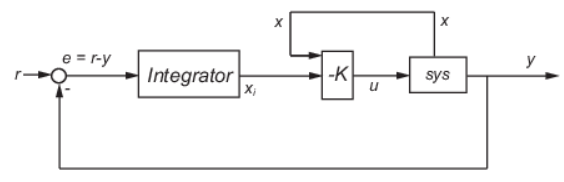
\includegraphics[width=0.5\linewidth]{LQI/LQI_loop.png}
    % \begin{tikzpicture}[
    %     block/.style = {draw, thick, rectangle,
    %                     minimum height=2em, align=center},
    %     sum/.style   = {draw, thick, circle,
    %                     minimum size=1.8em, inner sep=0pt},
    %     >=Stealth, thick, font=\small
    %     ]

    %     %─── Nodes (sum at origin; all others relative) ───────────────────────────
    %     \node[sum]                               (s)   at (0,0) {};
    %     \node[block, minimum width=3.0cm,
    %         right=1.8cm of s]                  (int)          {Integrator};
    %     \node[block, minimum width=1.8cm,
    %         right=2.0cm of int]                (K)             {$-K$};
    %     \node[block, minimum width=2.2cm,
    %         right=2.0cm of K]                  (sys)           {sys};
    %     \node[left=1.0cm of s]                   (r)             {$r(t)$};

    %     %─── Summing-junction sign labels ─────────────────────────────────────────
    %     \node[font=\scriptsize] at ($(s)+(-0.28,  0.22)$) {$+$};
    %     \node[font=\scriptsize] at ($(s)+( 0.00, -0.30)$) {$-$};

    %     %─── Key coordinates ──────────────────────────────────────────────────────
    %     \coordinate (outTip) at ($(sys.east)  + (1.4,  0  )$); % tip of output arrow
    %     \coordinate (topSys) at ($(sys.north) + (0,    1.3)$); % above sys
    %     \coordinate (topKw)  at (topSys       -| K.west);      % same height, above K.west
    %     \coordinate (botOut) at ($(outTip)    + (0,   -1.8)$); % below output
    %     \coordinate (botS)   at (s.south      |- botOut);      % below sum, same y

    %     %─── Forward path ─────────────────────────────────────────────────────────
    %     \draw[->] (r)   --                          (s);
    %     \draw[->] (s)   -- node[above]{$e = r-y$}  (int);
    %     \draw[->] (int) -- node[below]{$x_i$}       (K);
    %     \draw[->] (K)   -- node[below]{$u(t)$}          (sys);
    %     \draw[->] (sys) -- node[above]{$y(t)$}          (outTip);

    %     %─── State feedback (top): sys.north → up → left → down into K.north ──────
    %     \draw[->] (sys.north) -- (topSys) -- (topKw) -- (K.north);
    %     % "x" labels at both ends of the horizontal segment
    %     \node[above, font=\scriptsize] at ($(topKw)  !0.15!(topSys)$) {$x(t)$};
    %     \node[above, font=\scriptsize] at ($(topSys)!0.07!(topKw)  $) {$x(t)$};

    %     %─── Output feedback (bottom): outTip → down → left → up into s.south ─────
    %     \draw[->] (outTip) -- (botOut) -- (botS) -- (s.south);
    % \end{tikzpicture}
    \caption{Tracking loop with full state feedback control \citep{mathworks_lqi}.}
    \label{fig_LQI_loop}
\end{figure}

The optimal state feedback control law $u(t) = K \cdot x_{aug}(t)$ which minimizes the cost function, shown in equation \eqref{eq_LQI_cost_function}:
\begin{equation}\label{eq_LQI_cost_function}
     J(u) = \int ^{\infty}_0 (x_{aug}^{T}(t) Q\,x_{aug}(t) + u^{T}(t) R\, u(t))\, dt 
\end{equation} 
was computed using MATLAB \emph{lqi} function, for $R=10^{-9}$ and different $Q$ matrices, for the augmented system, where the state vector $x_{aug}(t) = \left[x(t) \, x_i(t) \right]^\intercal$ incorporates the state $x_i(t)$, which is defined as the integral of the tracking. The state weight matrix $Q$ had every element set to zero, except the entry corresponding to the integrated tracking error $x_i$, which was initially set to $10^3$, which resulted in a similar bandwidth to the tuned PID-F (figure \ref{fig_Bode_LQI_Qe3}), and then increased to $10^9$ (figure \ref{fig_Bode_LQI_Qe9}), for increased bandwidth, which, unlike with the large bandwidth PID-F controllers, the effect of the pole and zero (resonance and anti-resonance) observed on the low frequency was still highly smoothed, resulting in unitary gain at low frequencies, shown in figures \ref{fig_Bode_LQI_Qe9} through to \ref{fig_Platen_Displacement_Tracking_Error_LQI_Qe9}.

The code implementation can be found at the following GitHub repository \href{https://github.com/c-radicallis/Controlo_Plataforma_Sismica/blob/main/uniaxial_table_model/LQR%20Servo/LQI_servo.m}{location}.
    
\begin{figure}[H]
\begin{minipage}{0.49\textwidth}
    \centering
    
\includegraphics[width=\linewidth]{LQI/Sim_Res_Qe3/Bode_of_G_xT_xref.png}
    \caption{Bode plots of $G_ {xT/x_{\text{ref}}}(s)$ for the default controller, tuned PID-F, and optimal state-feedback controller with $Q=10^3$ (which results in a similar bandwidth to the tuned PID-F).}
    \label{fig_Bode_LQI_Qe3} 
\end{minipage}
\hfill
\begin{minipage}{0.49\textwidth}
    \centering
    
\includegraphics[width=\linewidth]{LQI/Sim_Res_Qe9/Bode_of_G_xT_xref.png}
    \caption{Bode plots of $G_ {xT/x_{\text{ref}}}(s)$ for the default controller, tuned PID-F, and optimal state-feedback controller with $Q=10^9$.}
    \label{fig_Bode_LQI_Qe9}
\end{minipage}
\end{figure}

\begin{figure}[H]
    \centering
    
\includegraphics[width=\linewidth]{LQI/Sim_Res_Qe9_tight/Response_Spectra.png}
    \caption{Response spectrum for fault normal. The response spectrum was obtained by sampling 500 frequencies logarithmically spaced between 0.1 and 30 Hz}%, and then applying a moving average filter with a window size of 25 points.}
    \label{fig_resp_spectrum_LQI_Qe9}
\end{figure}

\begin{figure}[H]
\begin{minipage}{0.49\textwidth}
    \centering
    
\includegraphics[width=\linewidth]{LQI/Sim_Res_Qe9_tight/Input_to_Servo.png}
    \caption{Input to servo}
    \label{fig_Input_to_Servo_LQI_Qe9}
\end{minipage}
\hfill
\begin{minipage}{0.49\textwidth}
    \centering
    
\includegraphics[width=\linewidth]{LQI/Sim_Res_Qe9_tight/Force_to_Platen.png}
    \caption{Force to Platen}
    \label{fig_Force_LQI_Qe9} 
\end{minipage}
\end{figure}
   
\begin{figure}[H]
\begin{minipage}{0.49\textwidth}
    \centering
    
\includegraphics[width=\linewidth]{LQI/Sim_Res_Qe9_tight/Platen_Acceleration.png}
    \caption{Platen acceleration}
    \label{fig_Platen_Acceleration_LQI_Qe9}
\end{minipage}
\hfill
\begin{minipage}{0.49\textwidth}
    \centering
    
\includegraphics[width=\linewidth]{LQI/Sim_Res_Qe9_tight/Platen_Displacement.png}
    \caption{Platen displacements}
    \label{fig_Platen_Displacement_LQI_Qe9}
\end{minipage}
\end{figure}

\begin{figure}[H]
\begin{minipage}{0.49\textwidth}
    \centering
    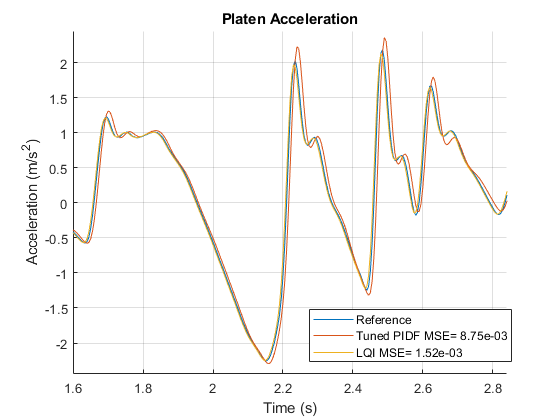
\includegraphics[width=\linewidth]{LQI/Sim_Res_Qe9_tight/Platen_Acceleration_zoom.png}
    \caption{Platen acceleration - Detailed view of the signals covering the period between 1.6 and 2.8 seconds}
    \label{fig_Platen_Acceleration_zoom_LQI_Qe9}
\end{minipage}
\hfill
\begin{minipage}{0.49\textwidth}
    \centering
    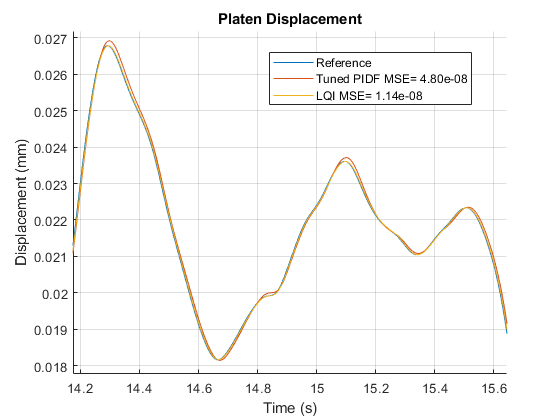
\includegraphics[width=\linewidth]{LQI/Sim_Res_Qe9_tight/Platen_Displacement_zoom.png}
    \caption{Platen displacements - Detailed view of the signals covering the period between 14.2 and 15.7 seconds}
    \label{fig_Platen_Displacement_zoom_LQI_Qe9}
\end{minipage}
\end{figure}

\begin{figure}[H]
\begin{minipage}{0.49\textwidth}
    \centering
    
\includegraphics[width=\linewidth]{LQI/Sim_Res_Qe9_tight/Platen_Acceleration_Tracking_Error.png}
    \caption{Acceleration tracking error}
    \label{fig_Platen_Acceleration_Tracking_Error_LQI_Qe9}
\end{minipage}
\hfill
\begin{minipage}{0.49\textwidth}
    \centering
    
\includegraphics[width=\linewidth]{LQI/Sim_Res_Qe9_tight/Platen_Displacement_Tracking_Error.png}
    \caption{Displacement tracking error}
    \label{fig_Platen_Displacement_Tracking_Error_LQI_Qe9}
\end{minipage}
\end{figure}

\subsubsection{LQG Servo Controller}\label{sec_LQG Servo Controller}

The implementation of the optimal control law requires the availability of all the systems states. For the system under analysis only the pltaform displacement and acceleration measurements are available, meaning that the whole state vector has to be estimated using an observer. To this end, the necessary software was developed in MATLAB using the function \emph{kalman} to compute the stationary Kalman state estimator (\emph{kest} in figure \ref{fig_LQG_inside_controller}) from the augmented system and the process and sensor noise covariance matrices, $Q_n$ and $R_n$ (set as identity matrices).  The optimal controller $k$ was computed using MATLAB \emph{lqi} function, for $R=10^{-9}$ and different $Q$ matrices (The state weight matrix $Q$ had every element set to zero, except the entry corresponding to the integrated tracking error $x_i$, which as initially set to $10^3$).

\begin{figure}[H]
\begin{subfigure}{0.41\textwidth}
    \centering
    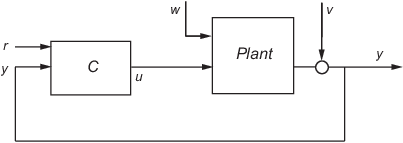
\includegraphics[width=\linewidth]{LQG/lqgtrack1.png}
    \caption{Full LQG loop} \label{fig_full_LQG_loop}
\end{subfigure}
\hfill
\begin{subfigure}{0.58\textwidth}
    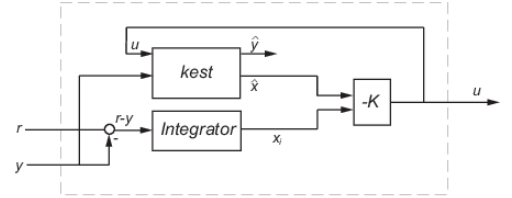
\includegraphics[width=\linewidth]{LQG/LQG_loop.png}
    \caption{Controller block diagram} \label{fig_LQG_inside_controller}
\end{subfigure} 
\caption{LQG control loop block diagram \citep{mathworks_lqgtrack}} \label{fig_LQG_loop}
\end{figure}

The MATLAB function \emph{lqgtrack} was used to compute the two-degree-of-freedom LQG servo controller C (as shown in figure \ref{fig_full_LQG_loop}, with its internal structure shown in figure \ref{fig_LQG_inside_controller}) by connecting the Kalman estimator \emph{kest} and the state-feedback gain \emph{k}. The code implementation can be found at the following GitHub repository \href{https://github.com/c-radicallis/Controlo_Plataforma_Sismica/blob/main/uniaxial_table_model/LQR%20Servo/LQG_servo.m}{location}. 

Simulations were run to verify the developed software was in working order for implementation in the real control system, or for use in improved Simulations when data of process and sensor noise covariance were to become available. The results shown in \ref{appendix:LQG Servo_Controller_Simulation_Results}, on  figures \ref{fig_resp_spectrum_LQG_Qe9} through to \ref{fig_Platen_Displacement_LQG_Qe9}, were very much identical to the ones obtained with the LQI controller, due to the fact that the state estimator output converged very fast.

\pagebreak
\subsection{LNEC's Control Strategy: OLI method}\label{sec_LNEC_method}
In this section the method used at LNEC for controlling the shaking table is described, and the results of numerical simulations from this method are used for comparison with the proposed controllers (PID-F and LQI).  

\subsubsection{The functioning of LNEC's \textit{Adapt} software}
As seen in the previous chapters, the use of a proportional controller for tracking the position reference signal does not produce the desired performance on the shaking table in terms of response spectrum. The method considered at LNEC to improve the shaking table performance comes in the form of combined open and closed loop control (Fig. \ref{fig_OLI}), whereby, before every test run, the proprietary software \emph{Adapt}, developed in LabVIEW, through a set of user-defined parameters, identifies the system transfer function, and then computes a modified reference signal, denoted as \emph{driver signal}, which is then used as the reference in the closed-loop control of the shaking table position.

The adaptation process starts with the definition of the input files on the project menu, shown in figure \ref{fig_Adapt_Project_Parameters}:
\begin{figure}[H]
    \centering
    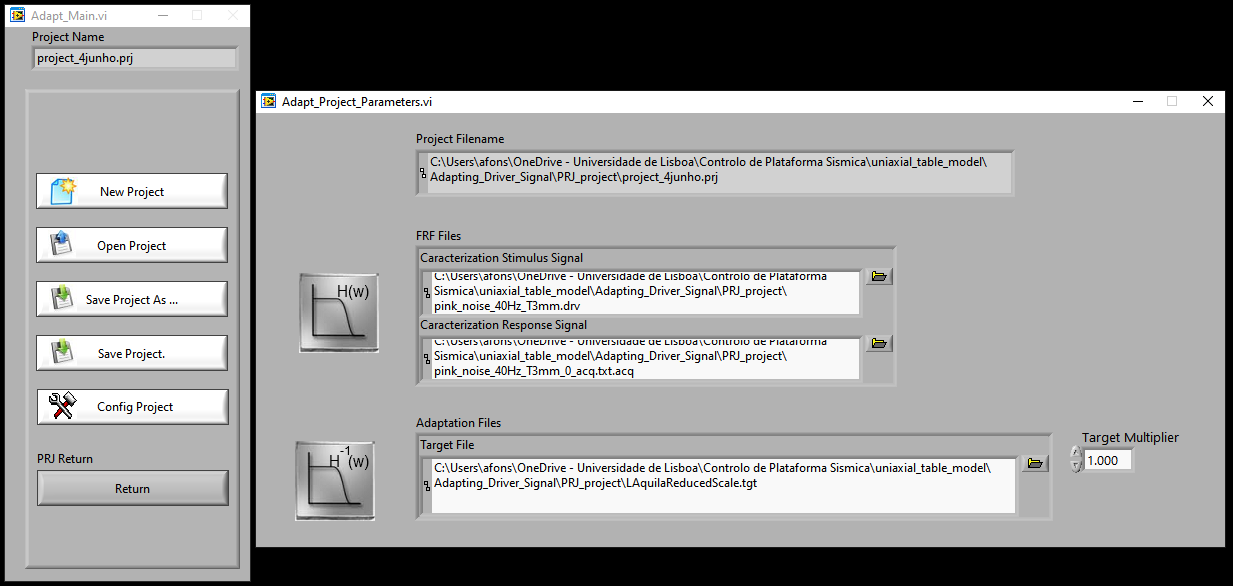
\includegraphics[width=1\linewidth]{Adapt/Adapt_Project_Parameters.png}
    \caption{Adapt Project Parameters menu - In this menu the user configures which files are used for determining the system's FRF, and the reference (or target) signal.}
    \label{fig_Adapt_Project_Parameters}
\end{figure}

Then, as the modification of the driver signal requires the identification of the frequency response function of the system, the user goes to the system identification menu, shown in figure \ref{Adapt_FRF_Parameters}. In this menu the user sets parameters which are used in the composition of a displacement signal from acceleration and displacement data acquired, usually, from a test run where 3 minutes of pink noise are used as input. The user can apply various filters to the acquired displacement and acceleration signals, and then choose how to synthesize both into a displacement signal. This is done to reject the inaccurate readings of position sensors at high frequencies, and of acceleration sensors at low frequencies, and combine the information of both to generate a more accurate displacement signal across the whole frequency spectrum.  The user also defines the settings for the computation of the FRF. 

The driver generation menu, shown in figure \ref{fig_Adapt_INV_Panel}, is used to generate new driver signals. It takes as inputs the original reference (referred to as \emph{target}), the driver signal used in the previous test run, it's measured displacements and acceleration at the shaking table, and user-defined parameters which affect which parts of the signal are modified, and by how much they're modified, it then outputs the driver to be used in following test run.
\begin{figure}
    \centering
    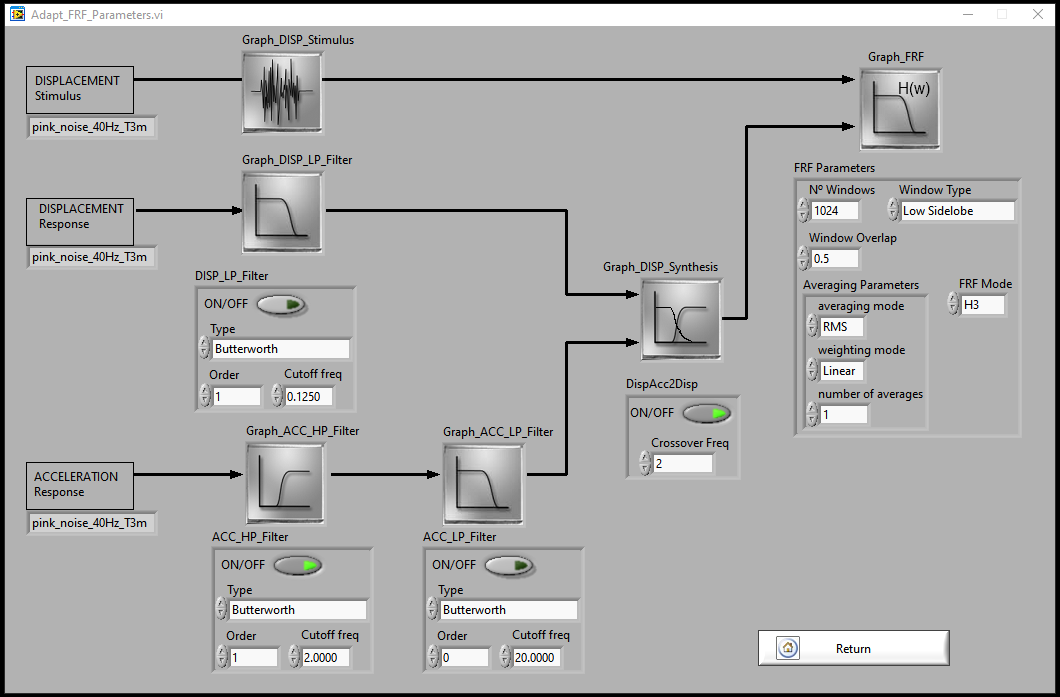
\includegraphics[width=\linewidth]{Adapt/Adapt_FRF_Parameters.png}
    \caption{Adapt FRF Parameters menu}
    \label{Adapt_FRF_Parameters}
\end{figure}

\begin{figure}
    \centering
    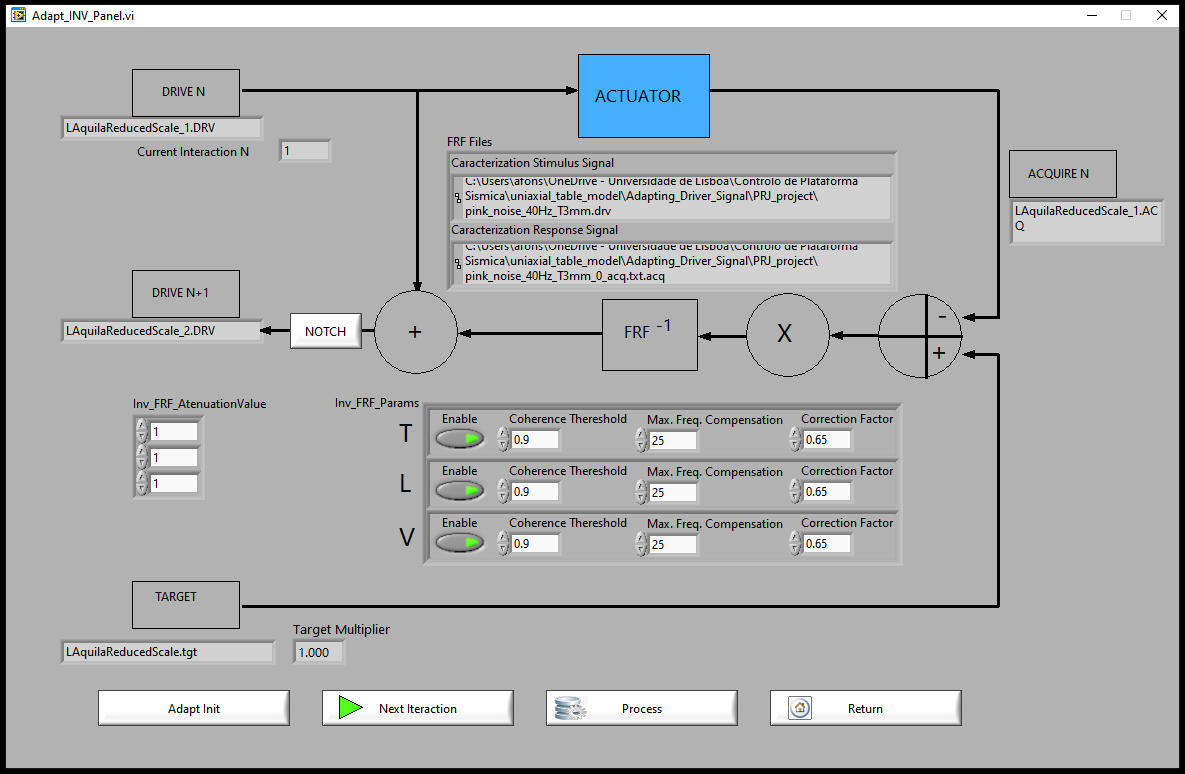
\includegraphics[width=\linewidth]{Adapt/Adapt_INV_Panel.png}
    \caption{Adapt INV Panel menu}
    \label{fig_Adapt_INV_Panel}
\end{figure}


\subsubsection{Simulating the driver adaptation process}

For the simulations in this section, the 2DOF system coupled to the platen with both masses set to 2000 kg, and the modal properties: $f_1 = 1.5 Hz$, $\zeta_1  = 0.02$, $f_2 = 6 Hz$, $\zeta_2 = 0.05$, was used to compute the results and evaluate the performance of the system with the LNEC's method

\paragraph{System Identification}
The first step in the driver adaptation process is the identification of the system (shaking platform and test specimen). A pink noise signal of 3 minutes duration was used as the identification input.

The input signal was obtained by converting a pink noise \emph{.drv} file (a proprietary format used with the LNEC software tools \emph{LNEC SPA} and \emph{Adapt}) into a format compatible with the MATLAB model, using a Python library that replicates core \emph{LNEC SPA} functionality. This library was also used to convert the simulation outputs (shaking table position and acceleration time histories) into \emph{.acq} files. The resulting driver and acquired data files were then provided as inputs to \emph{Adapt}, where the system FRF was estimated.

\paragraph{Generating the target files (.tgt)}
The \emph{Adapt} target file (.tgt) contains displacement and acceleration signals. In order to generate the target files, the original acceleration data of each earthquake was integrated twice using a trapezoidal rule, then, from the obtained displacement signal, the initial and final displacement values were used to compute the average drift velocity, which was then subtracted from the displacement signal, such that start and end position are at zero. Then, the signal was scaled to fit within the displacement range of shaking table (and the mathematical model).

\paragraph{Generating the adapted driver}
The first driver (driver zero) was generated using just the target file. This driver was then converted to text format using the previously mentioned Python functions, and then input into the Matlab model. From the simulation displacement output, the acceleration was computed using a second order central difference. This data was then written to \emph{.acq} format, and used, along with the target file, to generate driver 1  in \emph{Adapt.exe}. The same process was repeated to generate subsequent driver until the output response spectra was deemed to be sufficiently close to the target response spectra.

\paragraph{Discussion of Method \& Results}
For the seismic signal tested in this section (L'Aquila reduced scale earthquake), the response spectra from adapted drivers underperforms compared to the PID-F controller, and even more so when compared to the optimal controller. 

In figure \ref{Response_Spectra_better_id}, the identified FRF (figure \ref{bode_compare_better_id}) used for adapting the drivers  is closer to the model, resulting in a better adaptation of the driver signal, but it still requires 3 iterations to somewhat achieve the target response spectrum, and still doesn't perform as well as the optimal and PID-F controllers.

\begin{figure}[H]
\begin{minipage}{0.49\textwidth}
In figure \ref{Response_Spectra_2drivers}, the identified FRF (figure \ref{bode_compare}) used for adapting the drivers isn't as good as in the other case (figure \ref{bode_compare_better_id}), due to the settings defined by the user in \emph{Adapt}, and the resulting response spectrum after three iterations isn't very satisfactory. This shows the one of limitations of this method: It depends on the user to make the right decisions, but the user isn't perfect and there is no guarantee he'll opt for the best settings. Another limitation is the fact that the user does not have exact knowledge of the best settings, because unlike in this example, where the system is known and the FRF is made to match it (Figure \ref{bode_compare_better_id}), in reality this is not possible, leaving the user to make an informed guess based on the information displayed in \emph{Adapt} and past experience.
\end{minipage}
\hfill
\begin{minipage}{0.49\textwidth}
     \centering
    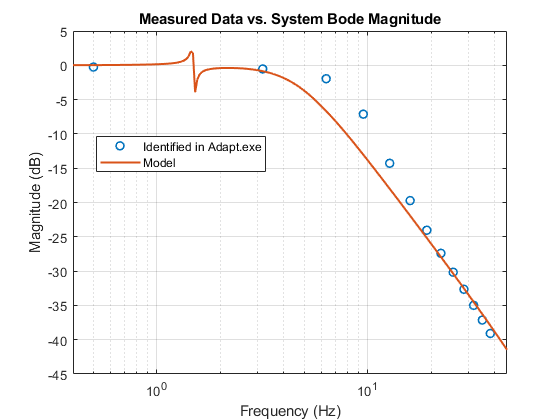
\includegraphics[width=\linewidth]{Adapt/bode_compare.png}
    \caption{Identified frequency response function from \emph{Adapt} (using "bad" settings) versus the model from Section \ref{Modelling Shaking Table Dynamics}}
    \label{bode_compare}
\end{minipage}
\end{figure}

\begin{figure}[H]
\begin{minipage}{0.49\textwidth}
    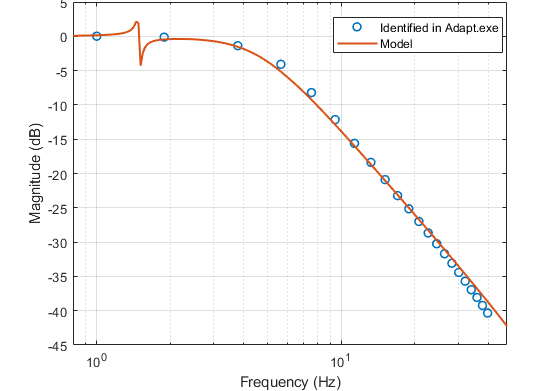
\includegraphics[width=\linewidth]{Adapt/bode_compare_better_id.png}
    \caption{Frequency response function of identified system using 1024 Low Sidelobe windows results in a rougher approximation of the transfer function, but handles noisy data better.}
    \label{bode_compare_better_id}
\end{minipage}
\hfill
\begin{minipage}{0.48\textwidth}
    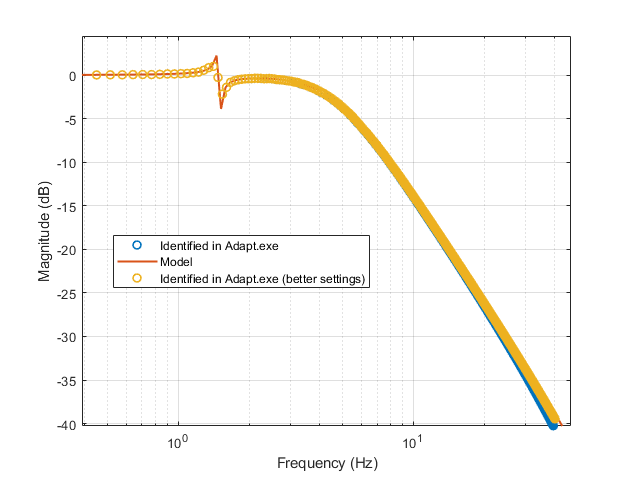
\includegraphics[width=\linewidth]{Adapt/FRFvsModelTF.png}
    \caption{Frequency response function of identified system using 20 Hanning windows results in a much better approximation of the transfer function, but likely wouldn't work as well if using noisy sensor data.}
    \label{FRFvsModelTF}
\end{minipage}
\end{figure}


\begin{figure}[H]
    \centering
    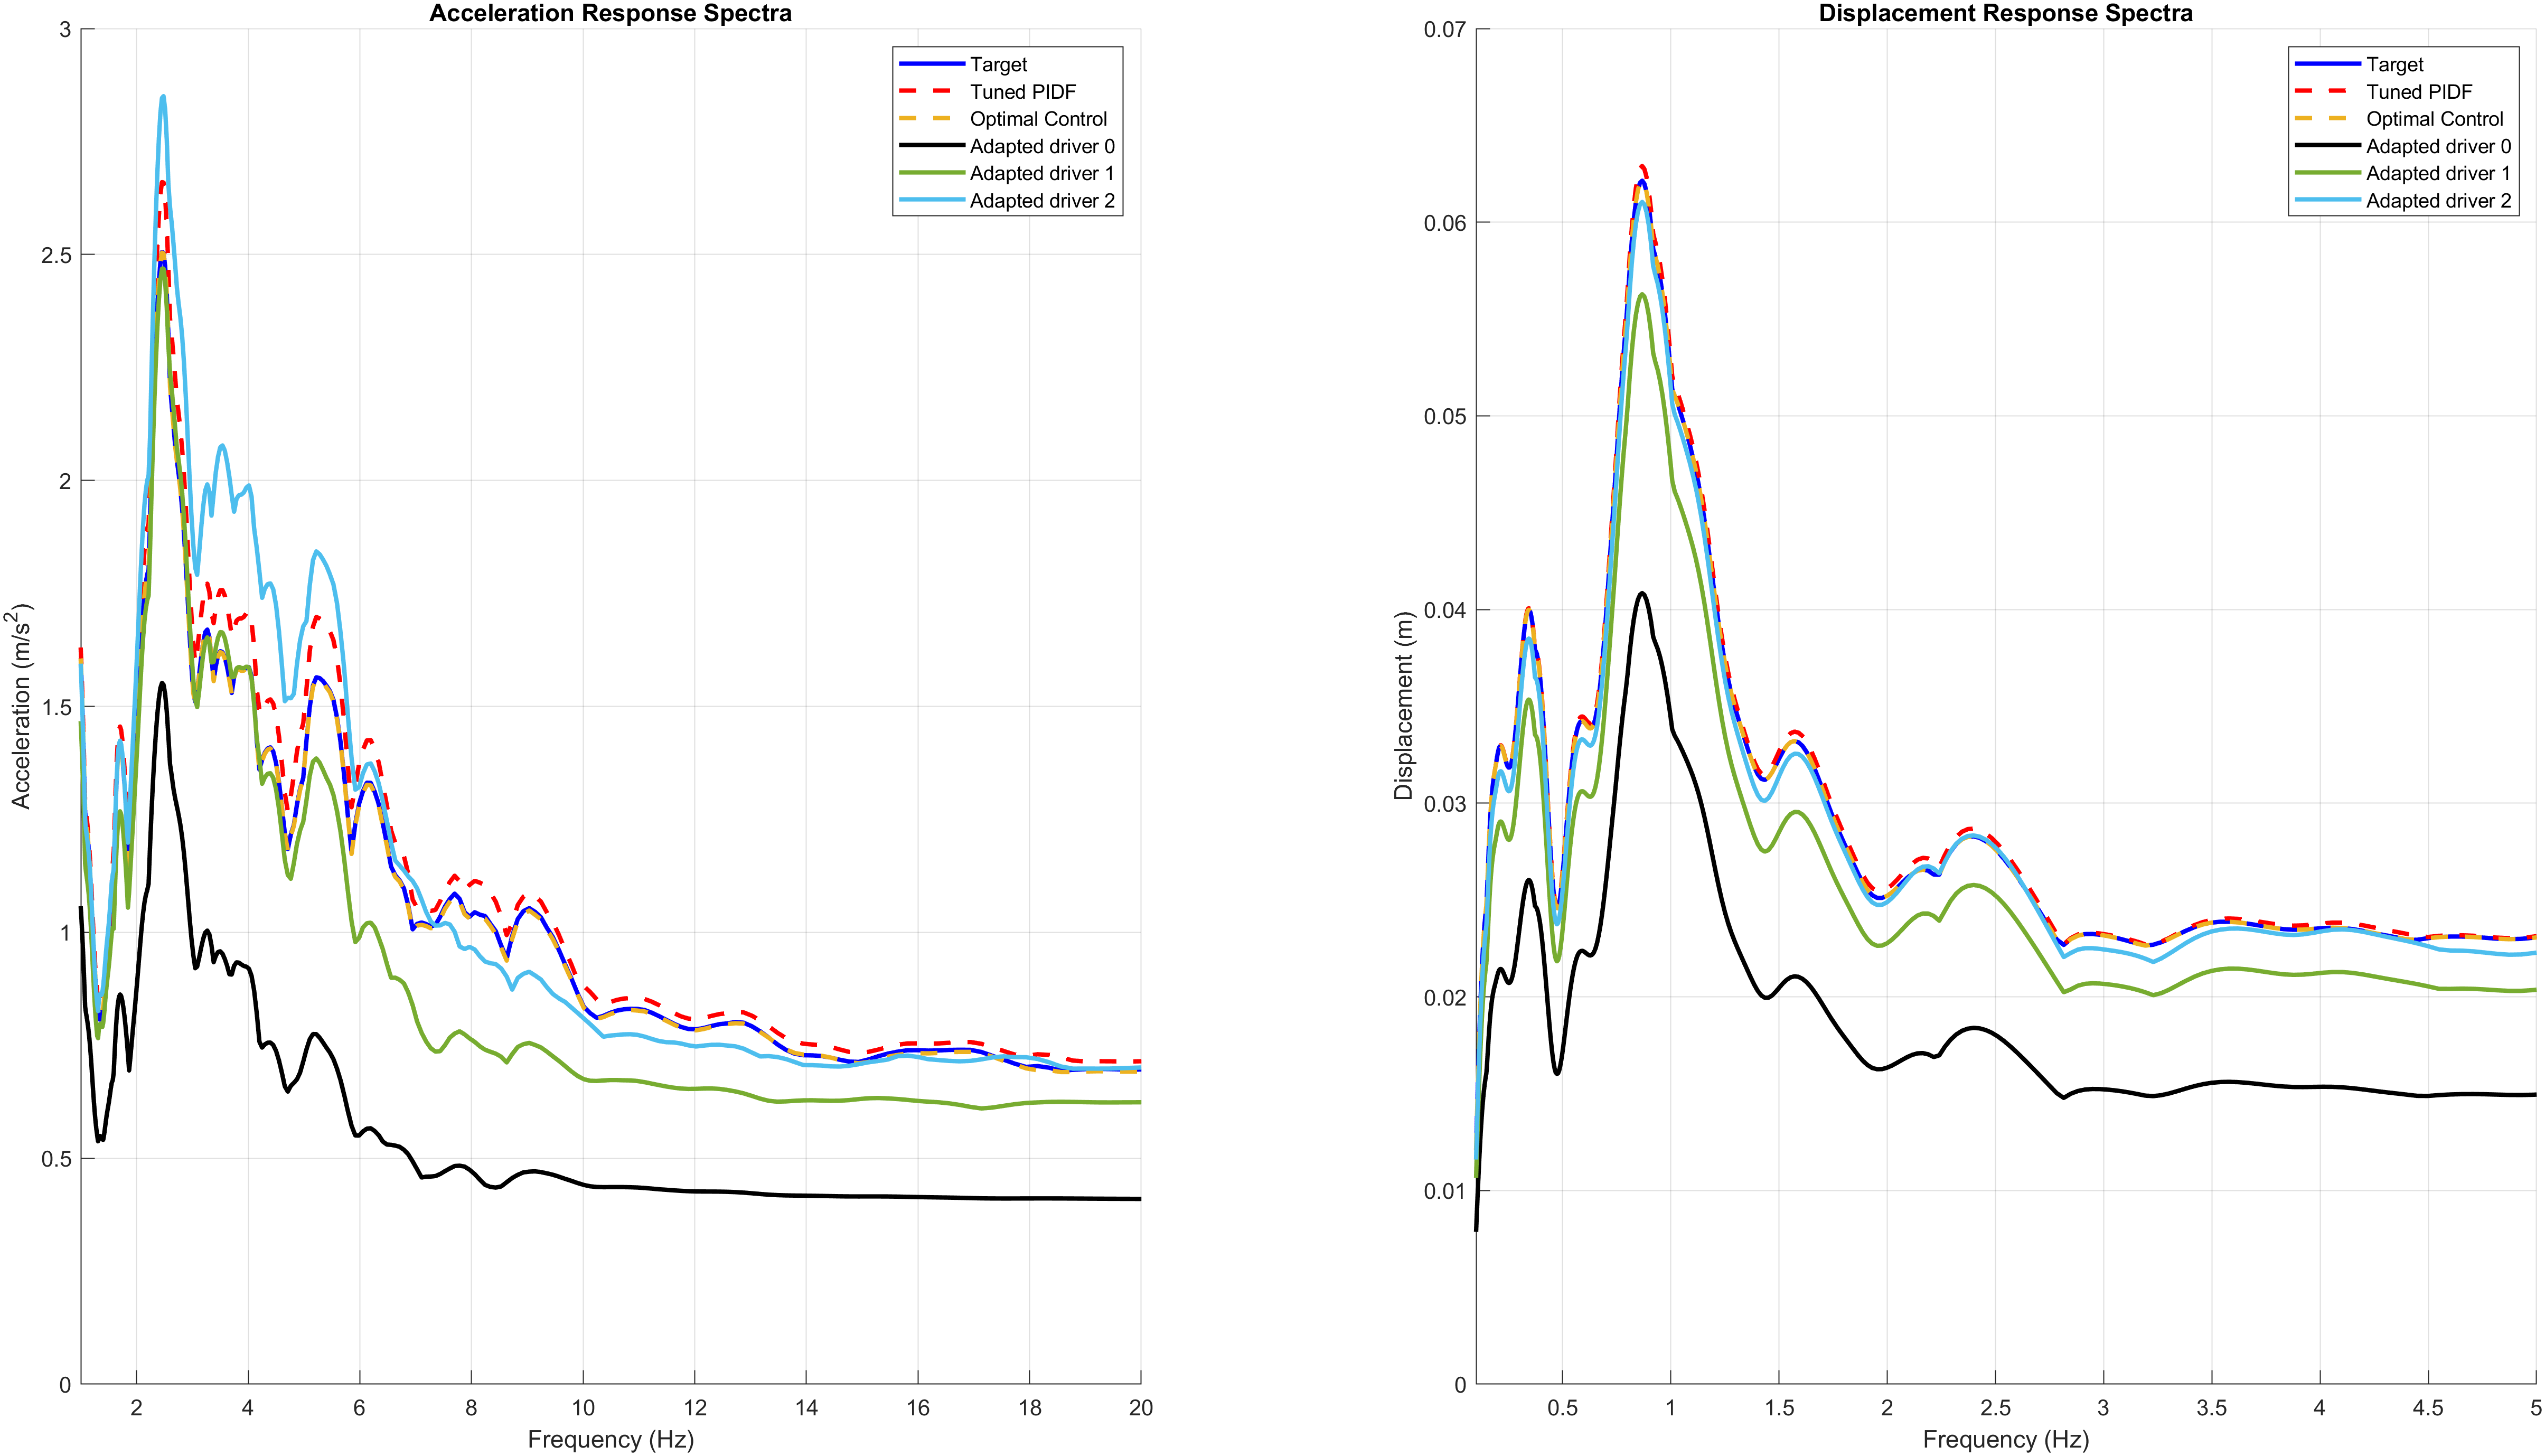
\includegraphics[width=1\linewidth]{Adapt/Response_Spectra.png}
    \caption{Target response spectrum and the resulting response spectrum from tuned PID-F, optimal controller, and the 3 iterations of adapted drivers resulting from FRF shown in figure \ref{bode_compare}.}
    \label{Response_Spectra_2drivers}
\end{figure}

\begin{figure}[H]
    \centering
    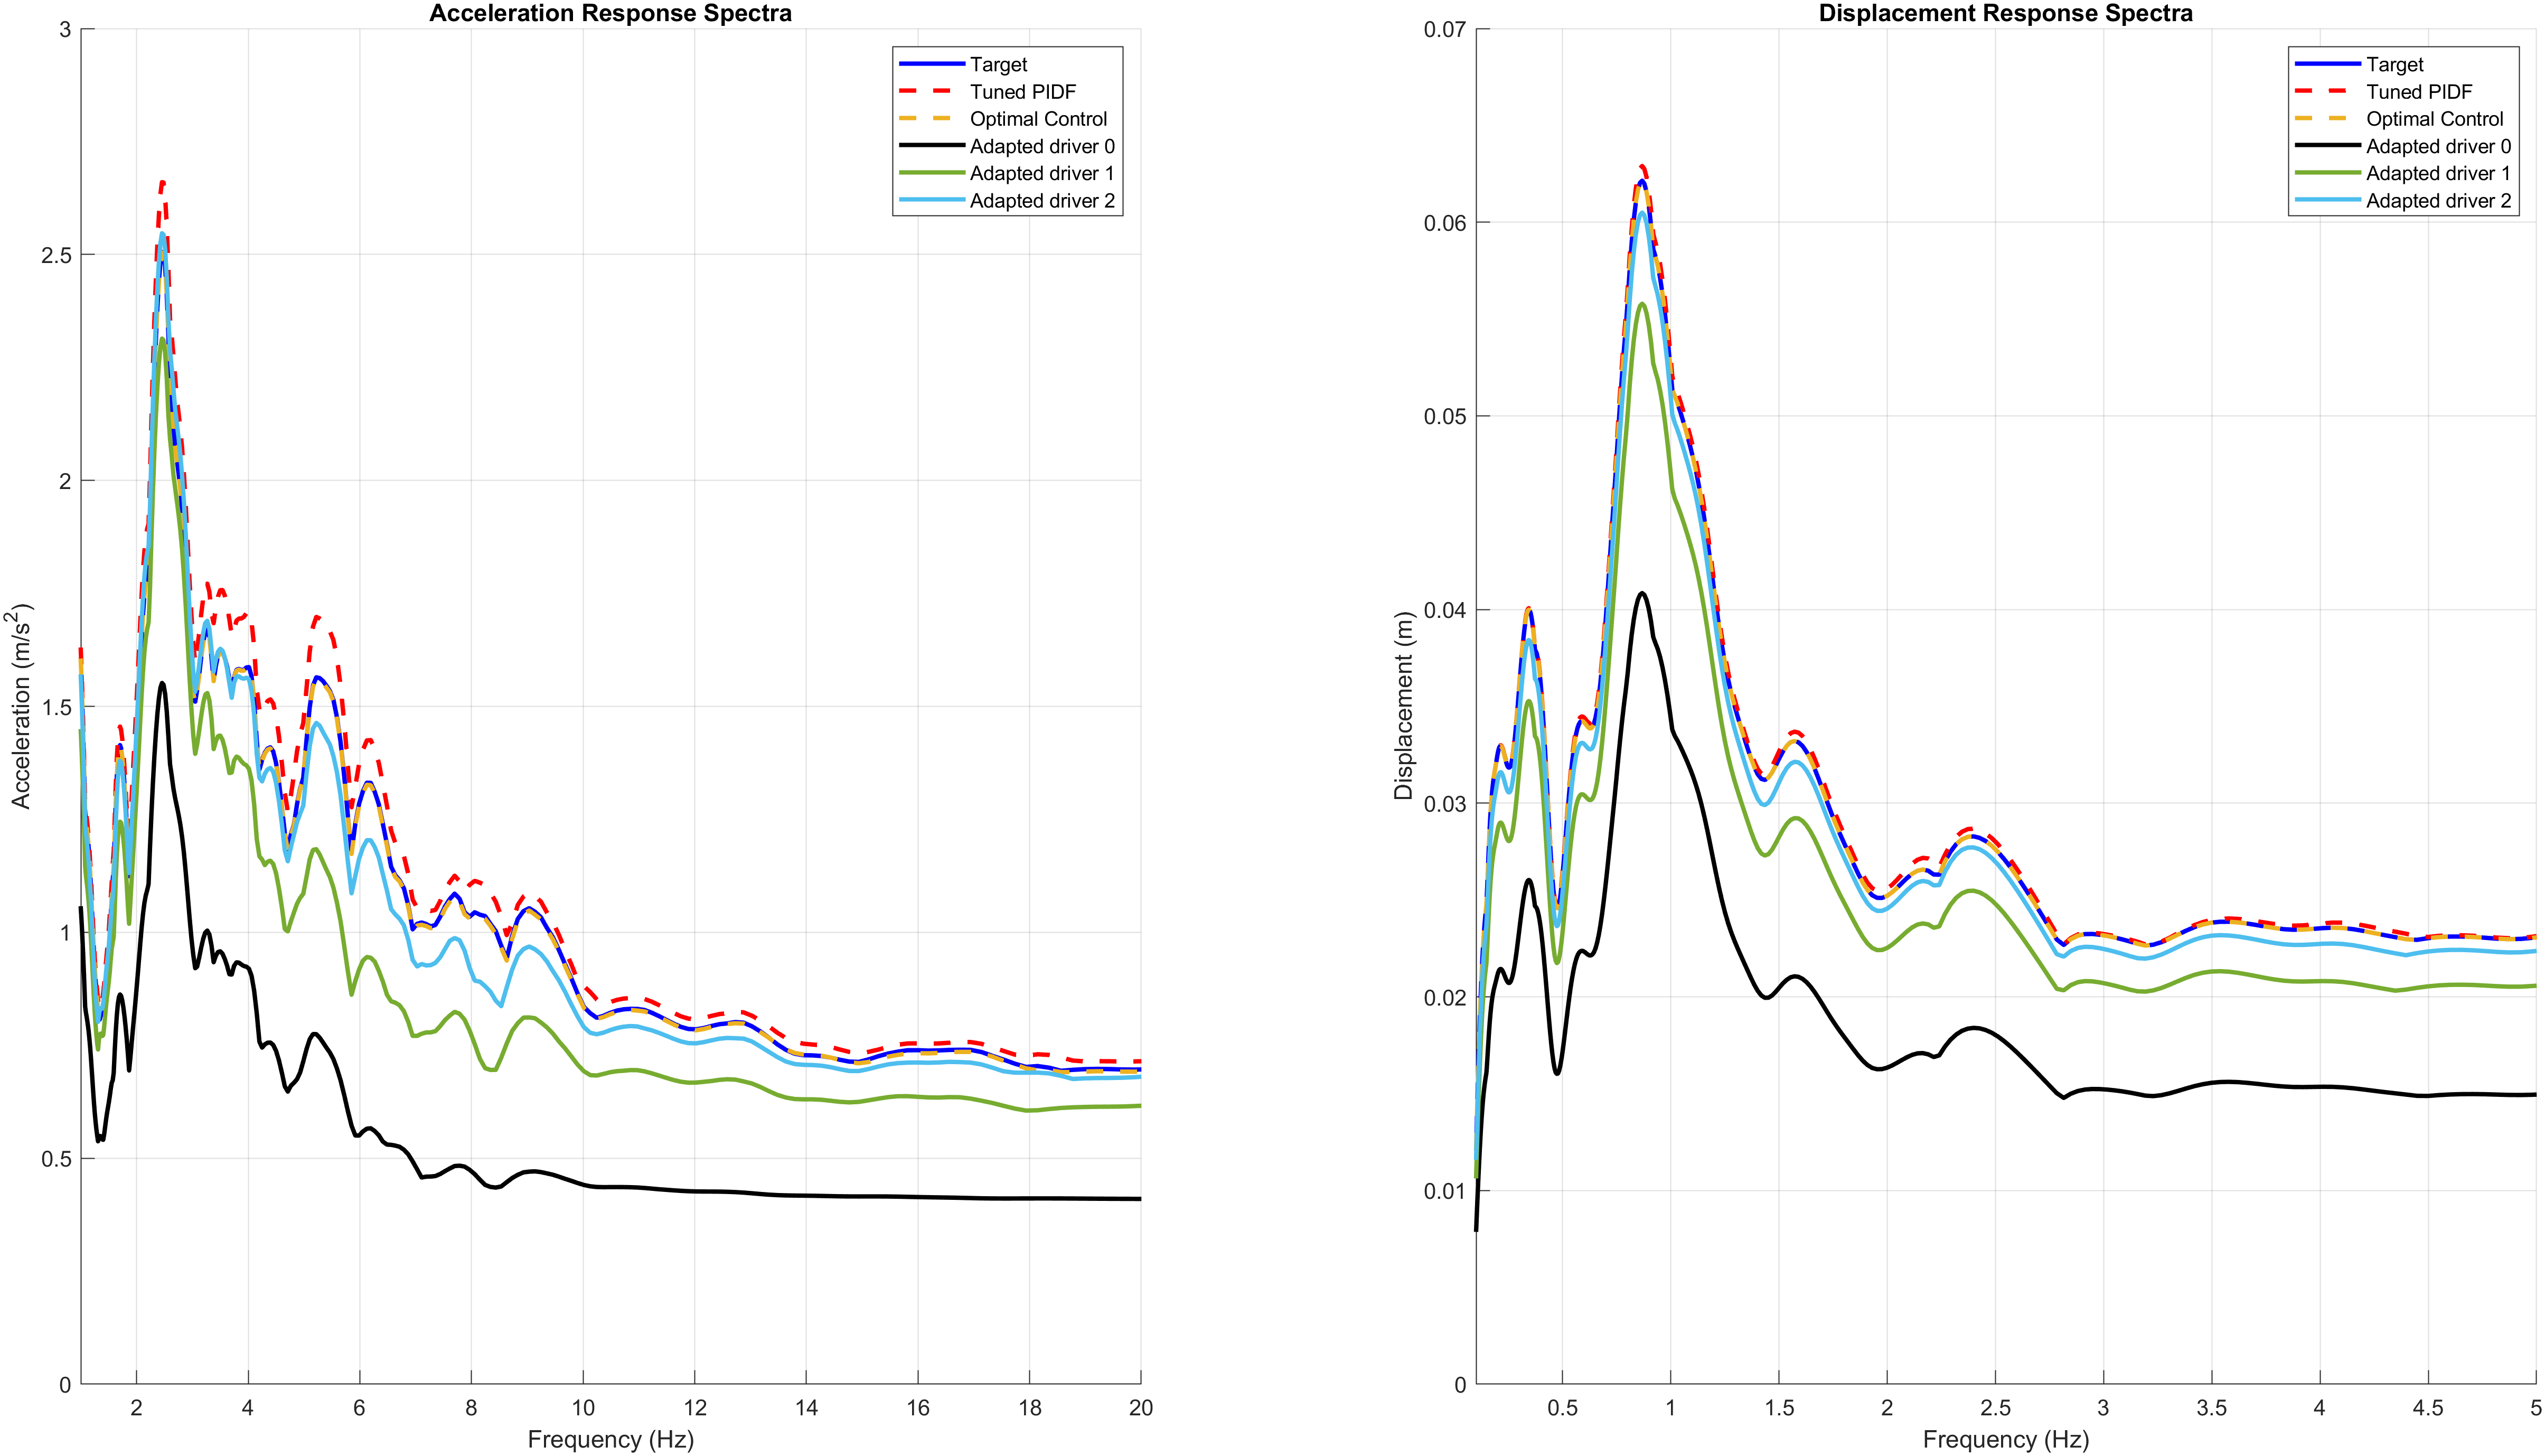
\includegraphics[width=1\linewidth]{Adapt/Response_Spectra_better_id.png}
    \caption{Target response spectrum and the resulting response spectrum from tuned PID-F, optimal controller, and the 3 iterations of adapted drivers resulting from FRF shown in figure \ref{bode_compare_better_id}.}
    \label{Response_Spectra_better_id}
\end{figure}

\section{Comparing Control Strategy Performance for Benchmark Seismic Signals}\label{sec_Comparing_Control_Strategies}

and the optimal controller with $Q=10^3$ (as in Figure \ref{fig_Bode_LQI_Qe3}). The code implementation can be found at the following GitHub repository \href{https://github.com/c-radicallis/Controlo_Plataforma_Sismica/blob/main/uniaxial_table_model/Adapting_Driver_Signal/sim_plot_adapted_drivers.m}{location}.

\begin{figure}[H]
    \centering
    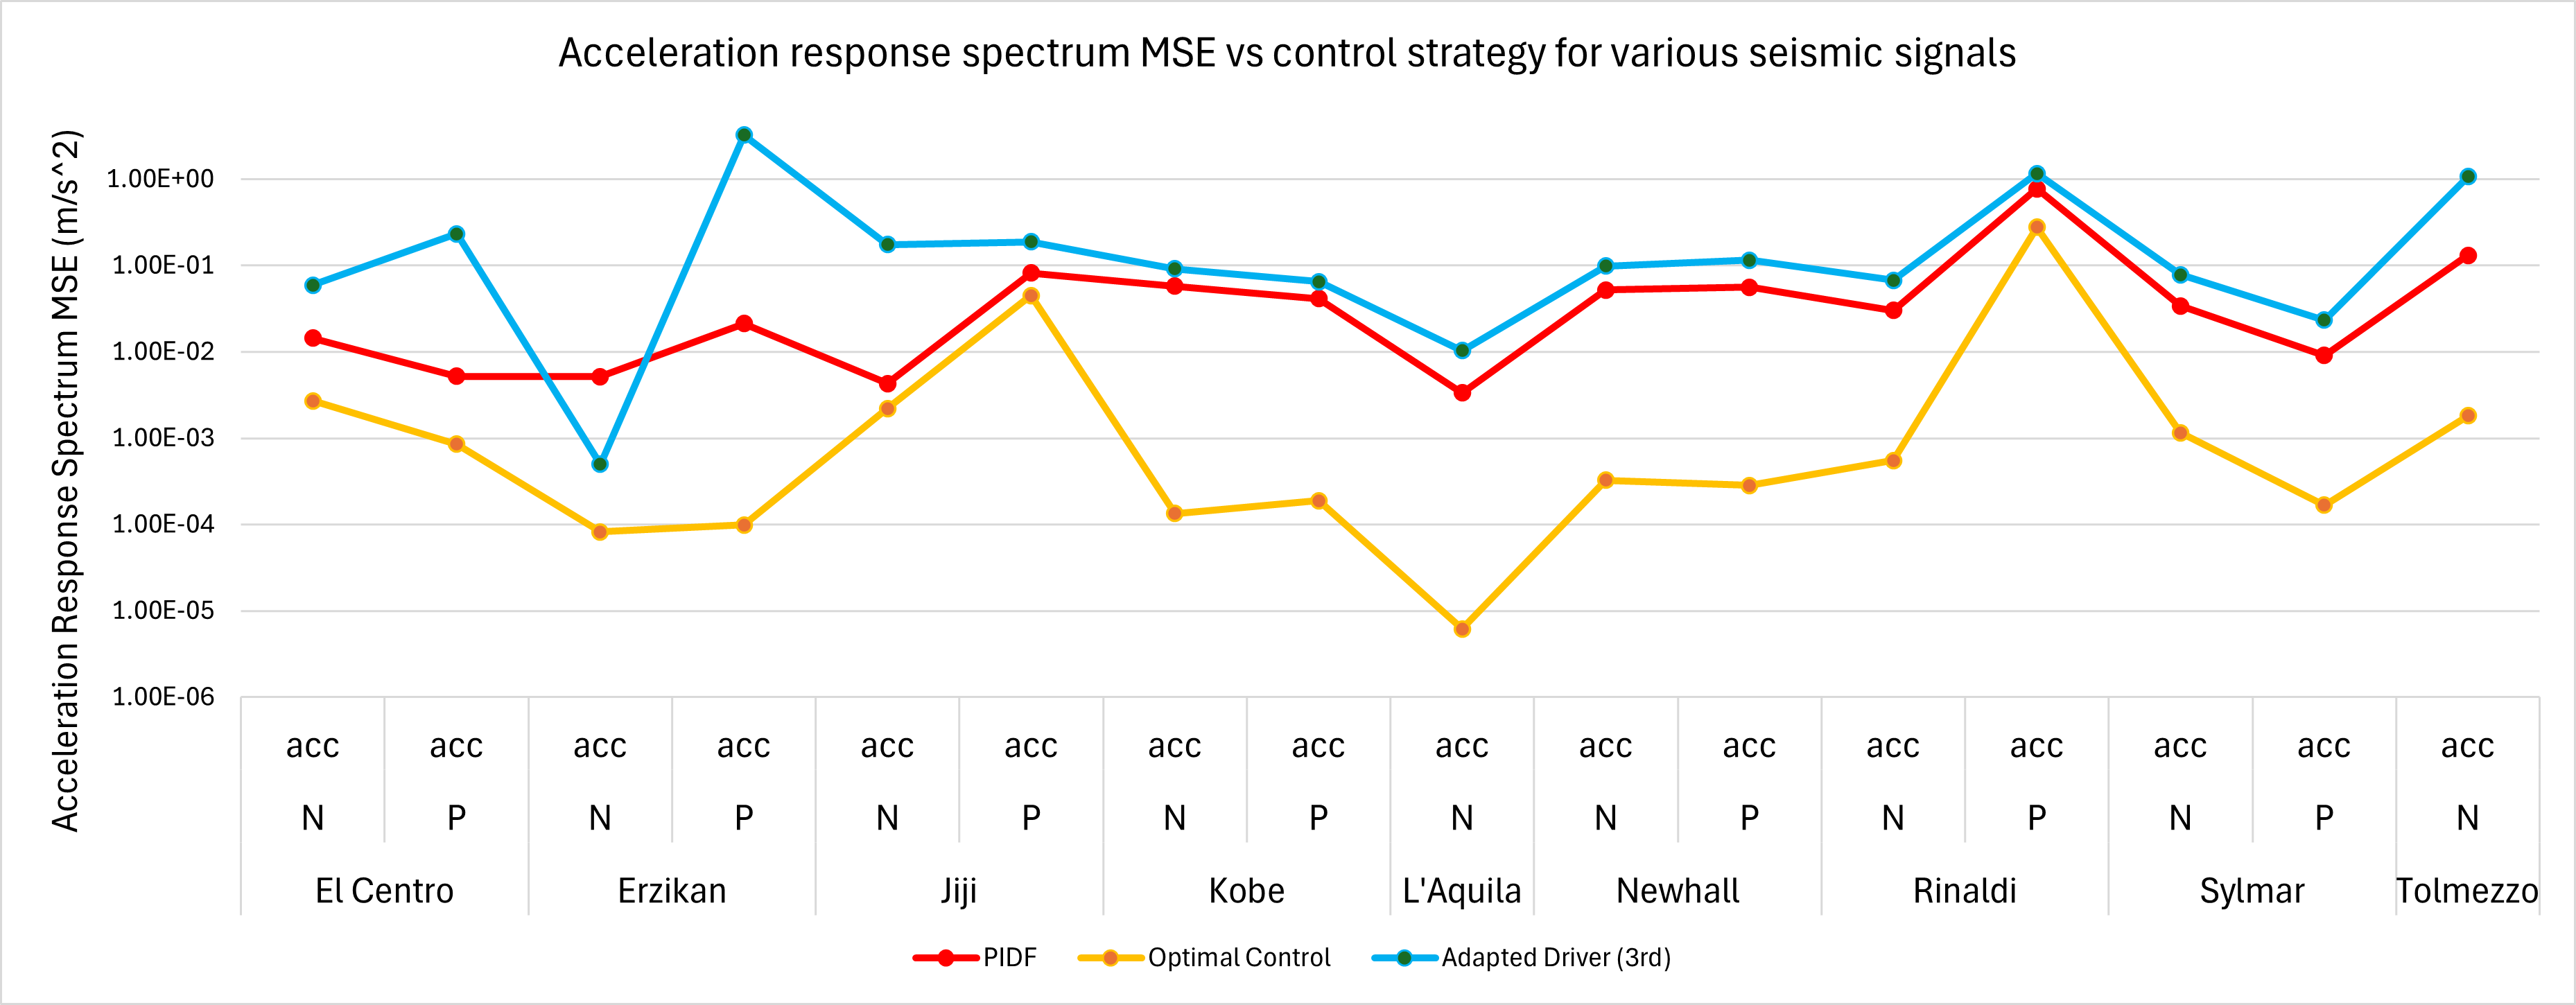
\includegraphics[width=\linewidth]{Adapt/excel_accel_resp_spectrum.png}
    \caption{Acceleration response spectrum MSE for various seismic signals. (For the Erzikan earthquake (figure \ref{erzikan_4th_N}), an additional driver adaption iteration was performed, and the results shown are for the resulting 4th driver)}
    \label{excel_accel_resp_spectrum}
\end{figure}

\begin{figure}[H]
    \centering
    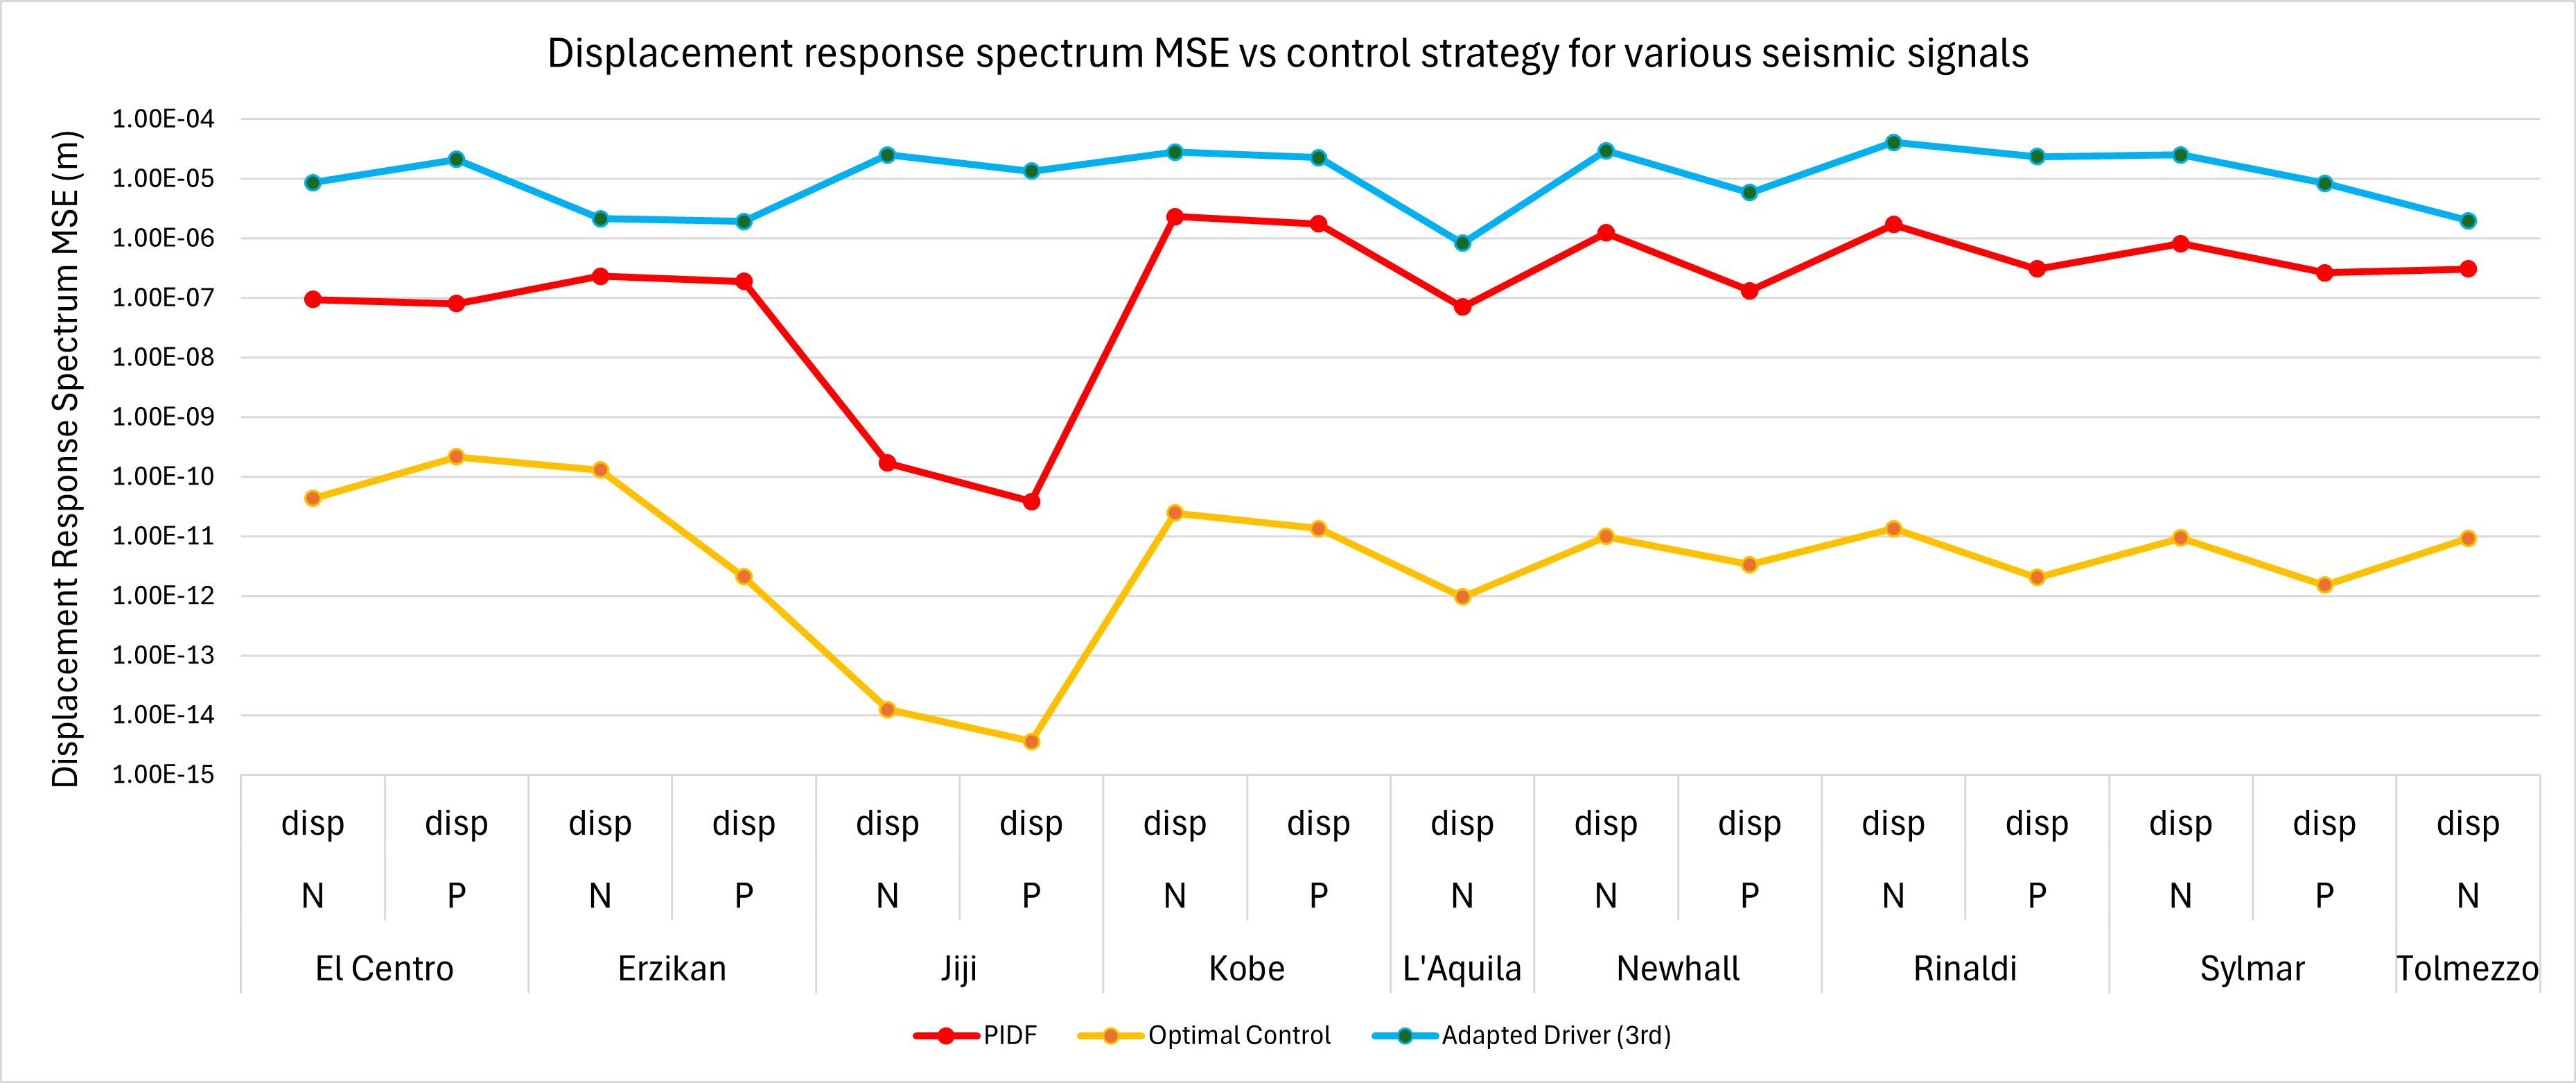
\includegraphics[width=\linewidth]{Adapt/excel_disp_resp_spectrum.png}
    \caption{Displacement response spectrum MSE for various seismic signals. (For the Erzikan earthquake (figure \ref{erzikan_4th_N}), an additional driver adaption iteration was performed, and the results shown are for the resulting 4th driver)}
    \label{excel_disp_resp_spectrum}
\end{figure}

\begin{table}[ht]
\centering
\begin{tabular}{cccc}
\hline
Control Strategy  & PID-F & Optimal Control & Adapted Driver (3rd)\\
\hline
Mean Acceleration MSE ($m/s^2$)    & \(8.27 \times 10^{-2}\) & \(2.09 \times 10^{-2}\) & \(4.17 \times 10^{-1}\) \\
Median Acceleration MSE ($m/s^2$) & \(3.20 \times 10^{-2}\) & \(4.39 \times 10^{-4}\) & \(9.48 \times 10^{-2}\) \\
Mean Displacement MSE ($m$) & \(5.97 \times 10^{-7}\) & \(3.01 \times 10^{-11}\) & \(1.62 \times 10^{-5}\) \\
Median Displacement MSE ($m$) & \(2.51 \times 10^{-7}\) & \(9.42 \times 10^{-12}\) & \(1.73 \times 10^{-5}\) \\
\hline
\end{tabular}
\caption{Comparison of mean and median response spectrum MSE for various seismic signals.}
\label{tab:metrics_comparison}
\end{table}


\begin{figure}[H]
    \centering
    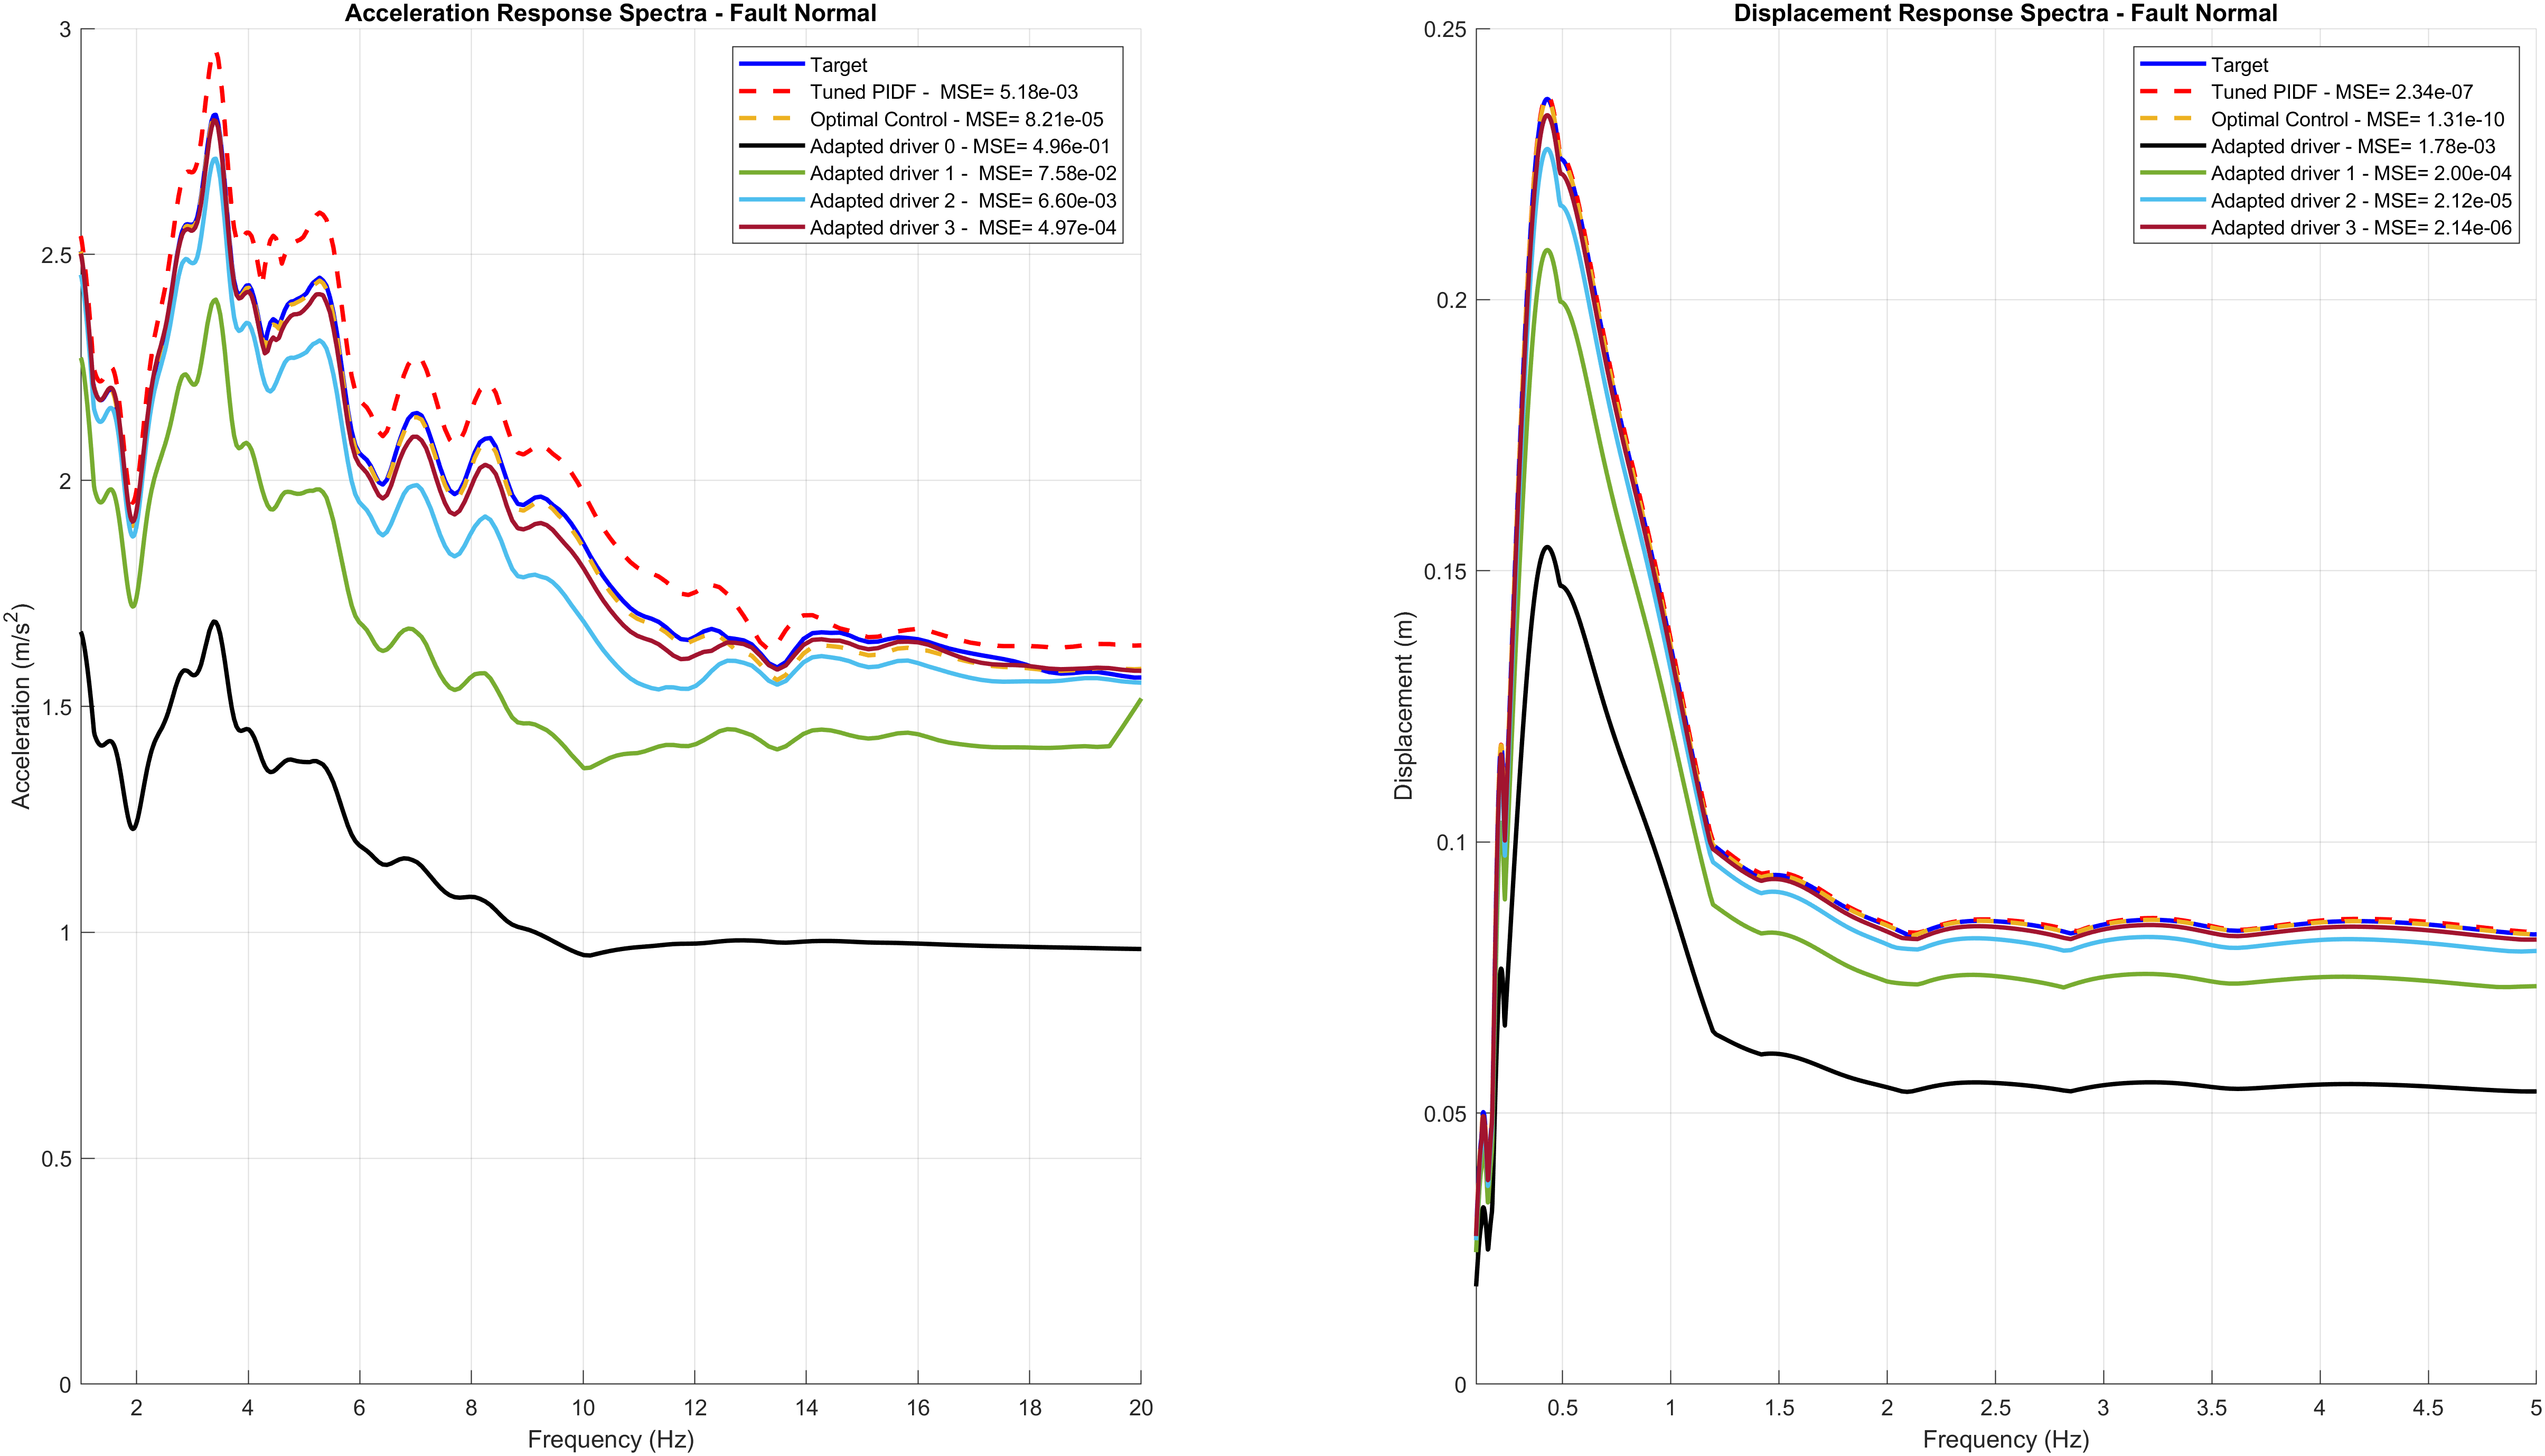
\includegraphics[width=1\linewidth]{Adapt/Erzikan_Response_Spectra_N.png}
    \caption{Erzikan fault normal response spectra. For this case a 4th adapted driver was computed, which yielded better results then the PID-F (unlike the 3rd driver used in every other performance comparison), but only in terms of acceleration response spectrum and in the fault normal direction.}
    \label{erzikan_4th_N}
\end{figure}

\section{ Conclusions: PID-F vs Optimal Control vs OLI Method}
%The first results indicate that the controllers previously studied offer superior performance in terms of response spectra compared to the adapted drivers, while also requiring less user intervention doing so. However, both the performance of the controllers and the adapted drivers depends on identifying the system, and the sensitivity of each method to quality of the identification is still unknown.
Regarding the analysis in sections \ref{sec_Tuned_PID-F} and \ref{sec_Optimal_Control}, optimal control results in a much more precise replication of the ground response spectra at low frequencies, unlike the tuned PID-F which exceeds the desired response spectra in the same band. However, the trade-off for this accuracy at lower frequencies is a response spectrum that falls short at higher ones.  The optimal controller can be tuned for increasingly larger cut off frequencies without undesired amplification at low frequency, unlike the PID-F, but the results of this is practice may differ from the simulation studies preformed using the current model.

The results indicate that the tuned controllers (PID-F \& Optimal) offer superior performance in terms of response spectra compared to the adapted drivers, while also requiring less user intervention doing so, with optimal control providing the best results in every instance. However, both the performance of the controllers and the adapted drivers depends on identifying the system, and the sensitivity of each method to quality of the identification is still unknown.

%%%%%%%%%%%%%%%%%%%%%%%%%%%%%%%%%%%%%%%%%%%%%%%%%%%%%%%%%%%%%5

\chapter{Experimental Validation}
% In order to experimentally validate the performance of the control strategies studied in \ref{Evaluating Controller Performance in Simulation Environment}, the two controllers were implemented in the LabVIEW software running in real time on 

As an alternative to testing on LNEC's uniaxial shaking table, as a result of its inoperability due to ongoing works in hydraulic and electrical system, an experimental facility consisting on an electrodynamic shaker was used to implement and test the necessary changes in the control software, and the proposed identification and control methods.

\section{ Measurement and Control Chain}
An experimental facility comprising a small-scale shaking table with dedicated hardware and software is used to validate the methodology. The measurement and control chain is depicted on figure \ref{fig_Experimental_facility} and, consists of:
\begin{itemize}
    \item Shaking Table, including a small-scale shaking table installed on a fixed base, along which it rolls over, driven by a Goodmans model 390A electrodynamic shaker, and a Linear Variable Differential Transformer (LVDT) measures the relative displacement of the platform;
    \item Conditioning and Control unit, with a hardware rack comprising all required signal conditioning and control components, including sensor signal conditioners and a National Instruments PXI Real-Time Controller integrated with a CompactRIO system featuring a Virtex-5 FPGA, enabling autonomous real-time execution of control and acquisition tasks;
    \item Data Acquisition System comprising a host PC, where the experimental setup is configured using the NI LabVIEW environment, including the implementation and supervision of the control strategy, the data acquisition set-up, as well as the measurement and visualization of the experimental results.
\end{itemize}

\begin{figure}[H]
    \centering
    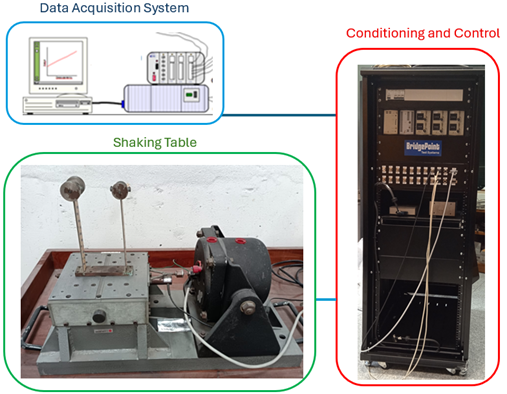
\includegraphics[width=0.6\linewidth]{experimental_validation/shaker_whole_system.png}
    \caption{Experimental facility}
    \label{fig_Experimental_facility}
\end{figure}

% \clearpage

One key advantage of this system framework is the modularity, since both data acquisition system and the condition and control rack can be deployed with other experimental set-ups. In particular, the system can be reused with the ST1D shaking table, where the proposed control strategies will be subsequently validated.

The system under study is a closed-loop control system, schematically illustrated in figure \ref{fig_Shaking table control loop}, comprising:
\begin{itemize}
    \item A controller, for which both a PID-F controller and an optimal LQI controller are considered in this study;
    \item A controlled system consisting of the shaking-table hardware, including its mechanical and electrical components, together with the top-mounted physical model. The control objective is that the output signal y, corresponding to the shaking-table motion, tracks the reference signal r, corresponding to the earthquake signal, as closely as possible.
\end{itemize}

\begin{figure}[H]
    \centering
    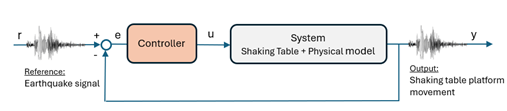
\includegraphics[width=0.9\linewidth]{experimental_validation/mini_table_control_loop.png}
    \caption{Shaking table control loop}
    \label{fig_Shaking table control loop}
\end{figure}

The control strategy currently implemented at LNEC is the OLI control approach. For the majority of applications, the PID controller parameters are tuned in advance for a specific test configuration and subsequently kept fixed throughout most experimental campaigns.

\section{Methodology}

This section details the methods with which the identification of the plant, tuning of controllers, and evaluation of controller performance is carried out. Firstly, the two-stage closed-loop identification method \citep{vandenhof1993} is applied to address the problem of consistent identification in closed-loop system. The following section describes the open-loop driver signal design process currently used at LNEC (which will serve as a baseline for controller performance evaluation), and two proposed developments for the shaking table control system. These developments consist on a systematic approach to designing optimized controllers of two different structures: a PID-F controller (for simplicity of implementation on the existing control system software and hardware), and an optimal controller (for greater performance).

% \subsection{ Calibration of Displacement Sensor}
% ver excel no computador da mesa sismica

% \subsection{ Calibration of Acceleration Sensor}
% \begin{enumerate}
%     \item In the acquisition/control software, set scaling to 1 and offset to zero
%     \item Place accelerometer vertically on a flat stationary surface (aligning the accelerometer measurement axis orthogonally to the acceleration of gravity) such that it will measure zero acceleration
%     \item Set the offset in the signal conditioner such that the output is zero
%     \item Place the accelerometer horizontally on a flat stationary surface, aligning accelerometer measurement axis with the acceleration of gravity, such that it will be sensing 1G
%     \item Set scaling in the conditioner and the software such that the output is 1G
% \end{enumerate}

\subsection{Identification of Electrodynamic Shaker}

The dynamic model identification of the plant is needed for tuning the controllers. To this end an identification experiment is carried out using a limited-band pink noise driver signal, with amplitude of approximately ±4 mm, with the controller set with proportional gain Kp=10, and data acquisition at 200 Hz. A sampling period of 5 ms is used throughout. The imperative of running experiments under closed-loop control poses additional challenges for identifying the plant (shaking table with physical model). To address the particularities of a closed-loop identification, the two-stage method \citep{vandenhof1993} illustrated in figure \ref{fig_two_stage_block_tikz} is applied. Firstly, the sensitivity function with controller, S0C, is identified by fitting a linear FIR model with 100 parameters (the order of the model just needs to be high enough to reproduce the noise-free control action, and high variance is not of concern). Then a Hammerstein-Wiener model is defined, using the previously identified FIR model as the linear block, and with the output nonlinearity equal to that of the physical system (saturation of the control action at known values), resulting in a more refined model for the sensitivity function. This function is then used to compute the noise-free control action ur, from which (by being uncorrelated with the output y) the plant G0 can now be estimated without bias introduced by the controller in the feedback loop.  The code implementation can be found at the following GitHub repository \href{https://github.com/c-radicallis/minimesa_data/blob/main/}{location}.

%\subsubsection{Applying Two-Stage Identification Method}

\begin{figure}[H]
    \centering
        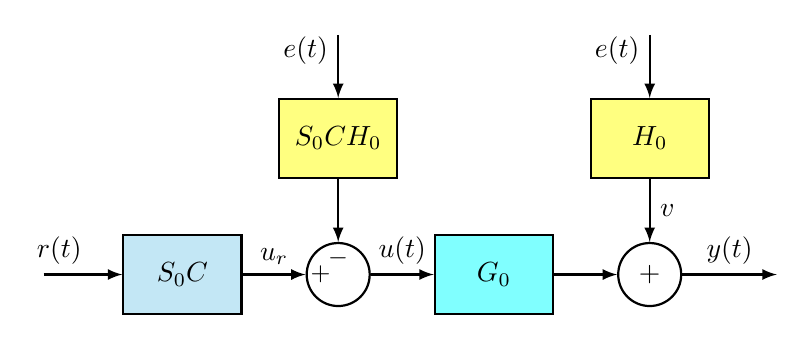
\begin{tikzpicture}[circ/.style = {draw, circle, minimum size=8mm, inner sep=0pt}, thick ]


        % S0C
        \node[draw, fill=SkyBlue!50, minimum width=15mm, minimum height=10mm ] (S0C) at (0,0) {$S_0 C$};
        %--- G0 -> sum_v ---
        \draw[-latex] ([xshift=-10mm]S0C.west) -- node[above, at start , xshift=2mm]{$r(t)$} (S0C.west);

        % sum_r1
        \node[circ , right=8mm of S0C ]  (sum_r1) {};
        \node[left=-1pt] at  (sum_r1.center){\small $+$};
        \node[above=-1pt] at (sum_r1.center){\small $-$};

        % G0
        \node[draw, fill=Cyan!50, minimum width=15mm, minimum height=10mm , right=8mm of sum_r1 ] (G0)    {$G_0$};

        % sum_v
        \node[circ, , right=8mm of G0 ]  (sum_v) {$+$};

        % H0
        \node[draw, fill=Yellow!50, minimum width=15mm, minimum height=10mm, above=8mm of sum_v ] (H0)  {$H_0$};

        \draw[-latex] (S0C) -- node[above]{$u_r$}(sum_r1);

        %--- e -> H0 -> v -> sum_v --- % H0
        \node[draw, fill=Yellow!50, minimum width=15mm, minimum height=10mm, above=8mm of sum_r1 ] (S0CH0)  {$S_0 C H_0$};
        \draw[-latex] ([yshift=8mm]S0CH0.north) node[left,yshift=-2mm]{$e(t)$} -- (S0CH0);
        \draw[-latex] (S0CH0) -- node[right]{} (sum_r1);

        %--- sum_r1 -> G0 ---
        \draw[-latex] (sum_r1) -- node[above]{$u(t)$} (G0);

        %--- G0 -> sum_v ---
        \draw[-latex] (G0) -- (sum_v);

        %--- e -> H0 -> v -> sum_v ---
        \draw[-latex] ([yshift=8mm]H0.north) node[left,yshift=-2mm]{$e(t)$} -- (H0);
        \draw[-latex] (H0) -- node[right]{$v$} (sum_v);

        %--- sum_v -> y output ---
        \draw[-latex] (sum_v) -- node[above]{$y(t)$} ([xshift=12mm] sum_v.east);


        \end{tikzpicture}
    \caption{Block diagram illustrating the two-stage method}
    \label{fig_two_stage_block_tikz}
\end{figure}

% \begin{enumerate}
%     \item \textbf{Identification of the sensitivity function $S_0$:}
%     \begin{itemize}
%         \item A linear FIR model with 100 parameters was fitted (the number of parameters was chosen arbitrarily for this stage).
%         \item A Hammerstein-Wiener model was then defined, using the previously identified FIR model as the linear block, and with the output nonlinearity equal to that of the physical system (saturation of the control action at known values), resulting in a refined model.
%     \end{itemize}
    
%     \item \textbf{Reconstruction of the control action isolated from noise effects ($\hat{u}_r$).}
    
%     \item \textbf{Identification of $G_0$:}
%     \begin{itemize}
%         \item Non-parametric identification indicated a 4th-order model.
%         \item A model with 4 poles and 3 zeros was fitted using the reconstructed control action and the measured output.
%     \end{itemize}
% \end{enumerate}

\subsection{Control Strategies}

\subsubsection{LNEC's driver signal iterative adaptation process}

This control technique is known as Online Iteration (OLI) [MTS Systems], as it iteratively modifies the command input on an individual sample-by-sample basis until the system response is close to the target. 
This method compensates the next drive signal with a drive correction signal which is computed from filtering the previous iteration error with the inverse model of the closed-loop frequency response function. The closed-loop frequency response function (FRF) is estimated via a nonparametric identification method by spectral analysis. To this end, the user interface of the driver iteration program allows many different settings for the identification. For the simulations of the OLI method, the identification used the same experimentally acquired data with the band-limited pink noise, and the FRF identification settings use Hanning window with the number of windows set to 8192 with 97\% overlap, and the FRF mode is set to H3. During the driver adaptation process, settings such as correction factor and maximum frequency compensation are adjusted as needed, while the coherence threshold is left at 90\%.
The closed-loop transfer function used in the simulations of the OLI method was estimated by direct identification (from signals “r” and “y”, resorting to figure \ref{fig_Shaking table control loop}), and its frequency response is shown in figure \ref{Fig6_Shaking table control loop frequency response with controllers optimized for the Tolmezzo earthquake}.

\subsubsection{ PID-F control strategy}

Taking into consideration the test procedure at LNEC (Figure \ref{fig_lnec_test_process_diagram}), where the identification is carried out each time the target signal is scaled up, one possible straightforward improvement would be to update the controller tune accordingly using this information. Another simple enhancement would be to add a filtered derivative term to the PI controller (making it a PID-F), since this should be of simple implementation in the existing version of the control software, as it is merely an extension of the existing controller structure, and allows more tunability. This is precisely what was done: optimize the PID-F gains to the identified plant dynamics. 
The simulations with the PID-F controller use the plant model resulting from the two-stage identification and the controller itself to close the loop.

\subsubsection{LQI control strategy}

The controllable canonical form state space representation of the plant transfer function obtained via the closed-loop two stage method identification is used in the minimization of the LQI cost function:
\begin{equation}
 J = \sum_{0}^{\infty}{{x\left(t\right)}^\intercal Q}x(t)+{u\left(t\right)}^\intercal R u(t) dt
\end{equation}
where Q and R have appropriate dimensions, with R=1 and Q being a diagonal matrix where each parameter was found via Nelder-Mead simplex algorithm \citep{lagarias1998} in order to minimize the acceleration response spectrum MSE for the seismic signal on test, computed for 100 logarithmically spaced points between 0.1Hz and 30Hz. The optimal state feedback control law is given by u(t) = K [x(t) xi(t)]T, with xi(t) being the integral of the tracking error

The simulations with the LQI controller use the plant model resulting from the two-stage identification, and the controller itself to close the loop.

\subsection{Performance Evaluation}

A set of recorded earthquake ground-motion time histories covering a wide range of seismic characteristics are considered in this study, namely \citep{narasimhan2006}: i) 1940 Imperial Valley earthquake, El Centro Fault Normal (FN) and Fault Parallel (FP) records; ii) 1992 Erzikan earthquake, Erzikan North-South (NS) and East-West (EW) record; iii) 1995 Kobe earthquake, Kobe NS and EW records; iv) 2009 L'Aquila earthquake; v) 1994 Northridge earthquake, Newhall FN and FP records; vi) 1994 Northridge earthquake, Rinaldi FN and FP records; vii) 1994 Northridge earthquake, Sylmar FN and FP records; viii) 1976 Friuli earthquake, Tolmezzo record. To ensure that the imposed inputs remained within the displacement capacity of the shaking table, appropriate scale factors were computed by taking the quotient of maximum desired displacement of 4 mm with the maximum displacement of any direction of the seismic signal (rounded to 3 decimal places) and then applied to the ground-motion signals. 
The performance of each control method is evaluated through the acceleration and displacement response spectrum mean squared error (MSE) for every input action described in the previous section. The acceleration response spectrum is computed from 0.1 Hz to 30 Hz for 500 logarithmically spaced points, and the displacement response spectrum is computed for the same frequencies, however, for only the first 344 points, equating to a range from 0.1 Hz to 5.04 Hz.


% \subsection{Checking the shaker and table for mechanical issues}

% Given the unexpected nonlinearities found during the identification (figures \ref{fig_sine_nonlinearity} and \ref{fig_square_nonlinearity}), the power to the shaker was turned off and the table was directly actuated by hand through its entire travel, and with direction changes, in order to feel for any binding or play in the system.  Since binding could be felt at certain points in the travel, both the shaker and the table slideways were disassembled to check for issues.

% \begin{figure}[H]
% \begin{minipage}{0.49\textwidth}
%         \centering
%     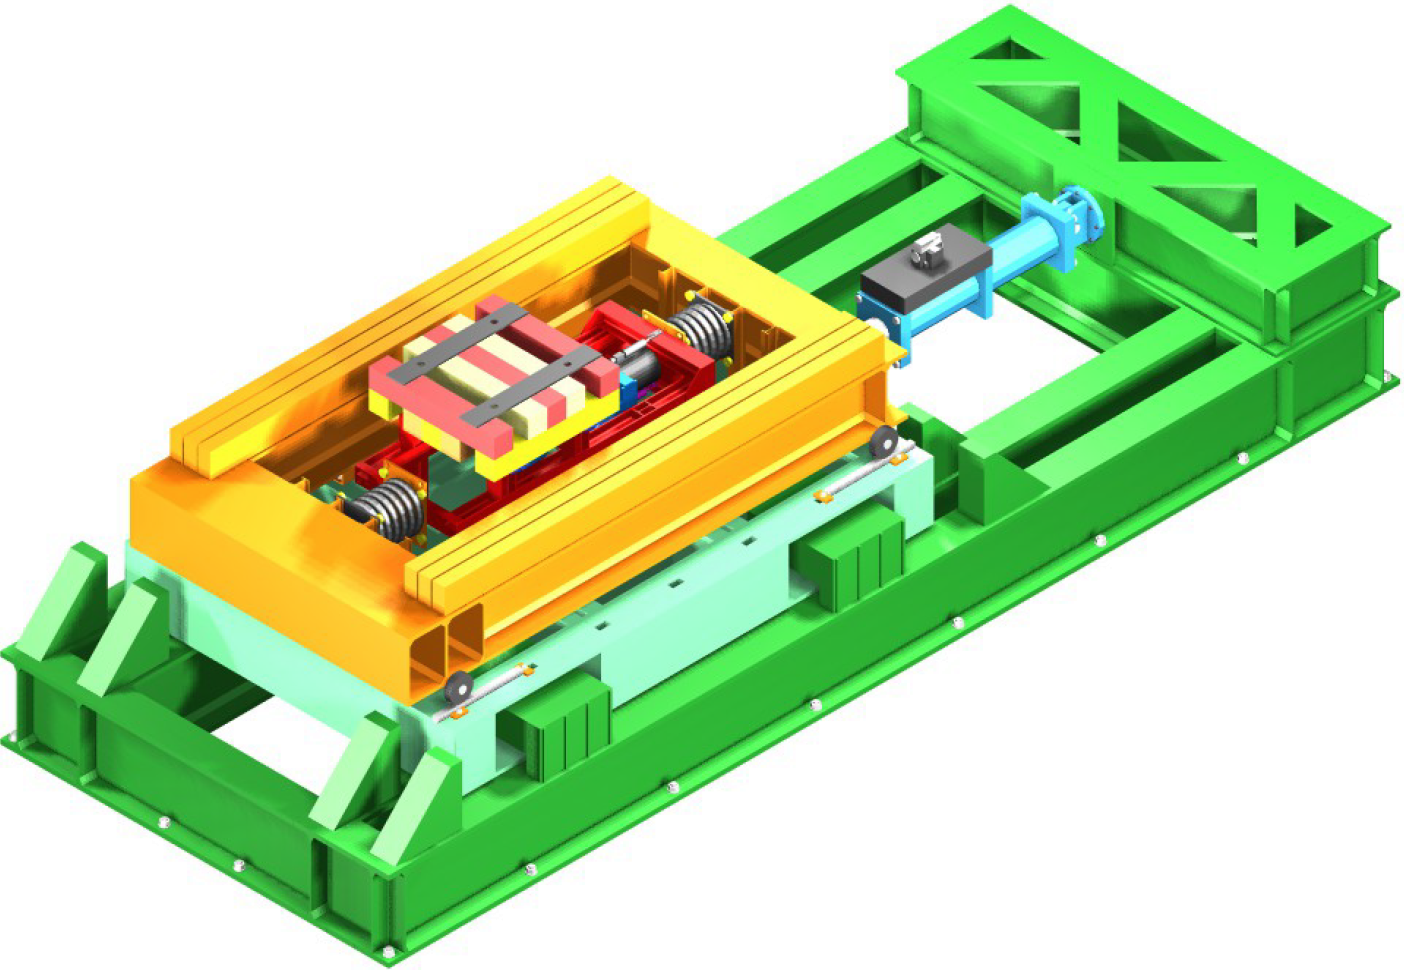
\includegraphics[width=\linewidth]{Figures/capa.png}
%     \caption{Caption}
%     %\label{fig_sine_nonlinearity}
% \end{minipage}
% \hfill
% \begin{minipage}{0.49\textwidth}
%     \centering
%     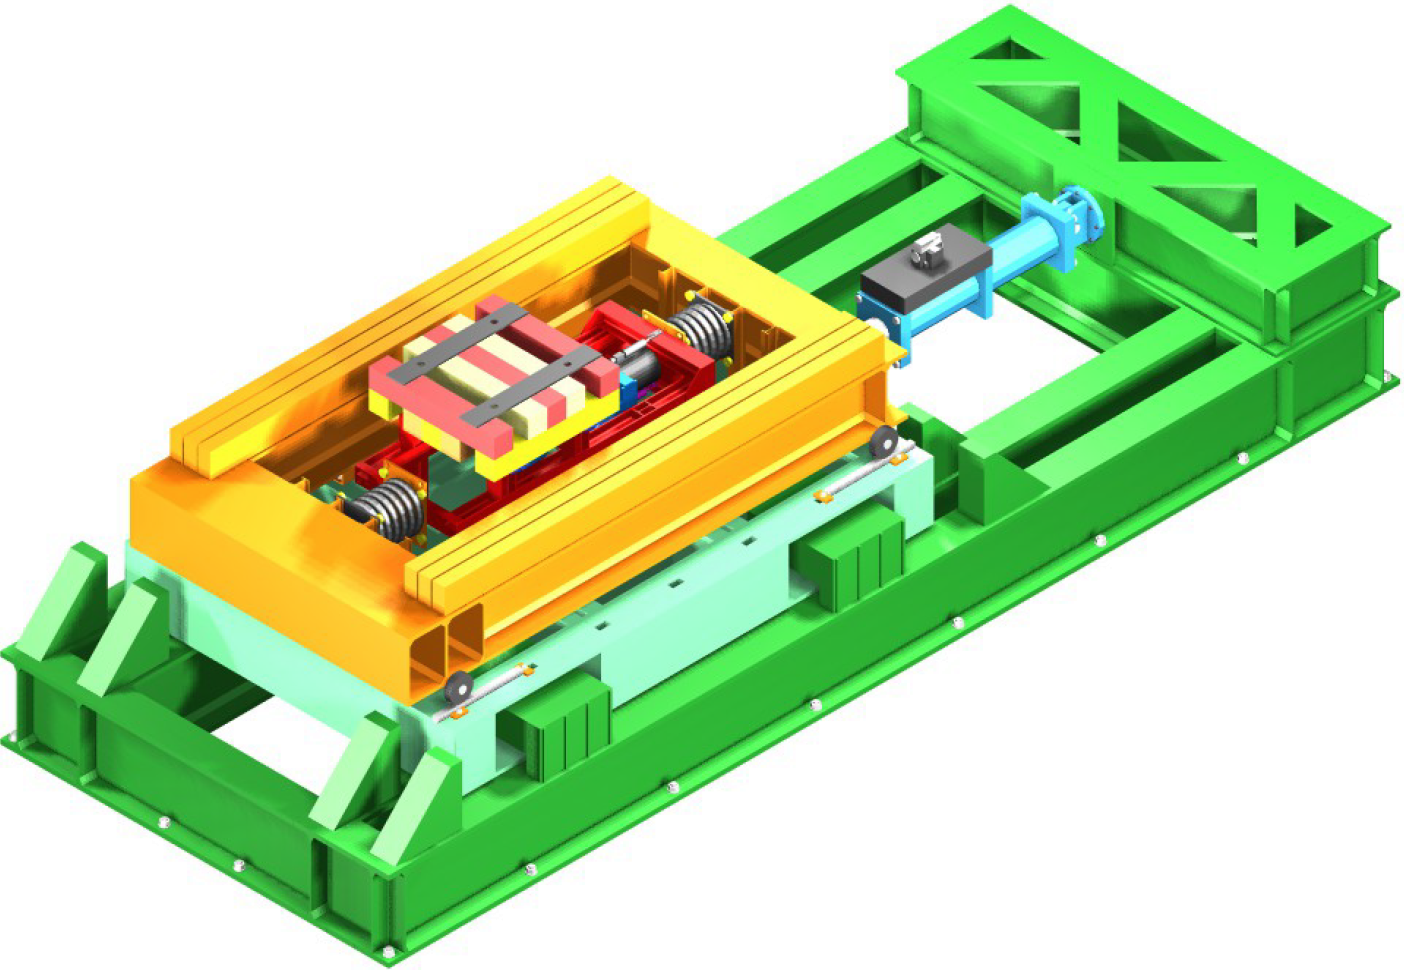
\includegraphics[width=\linewidth]{Figures/capa.png}
%     \caption{another Caption 2}
%     %\label{fig_square_nonlinearity}
% \end{minipage}
% \end{figure}

% With the table disconnected from the shaker, it was once again actuated by hand and appeared to be running smooth, without any binding or play. Regardless, the slideways were cleaned, visually inspected, lubed, and reassembled.

% With the table disconnected from the shaker, while actuating the shaker shaft by hand through its travel, often times binding could be felt. With the shaker disassembled, it was verified that a flat helical spring which connects the actuator shaft assembly to the shaker chassis had the come loose, and this may have been the source of the issue. Given the interface materials, cyanoacrylate glue was deemed suitable for the job, and the spring was bonded in its original place. No other obvious issues were found.

% \begin{figure}[H]
% \begin{minipage}{0.49\textwidth}
%         \centering
%     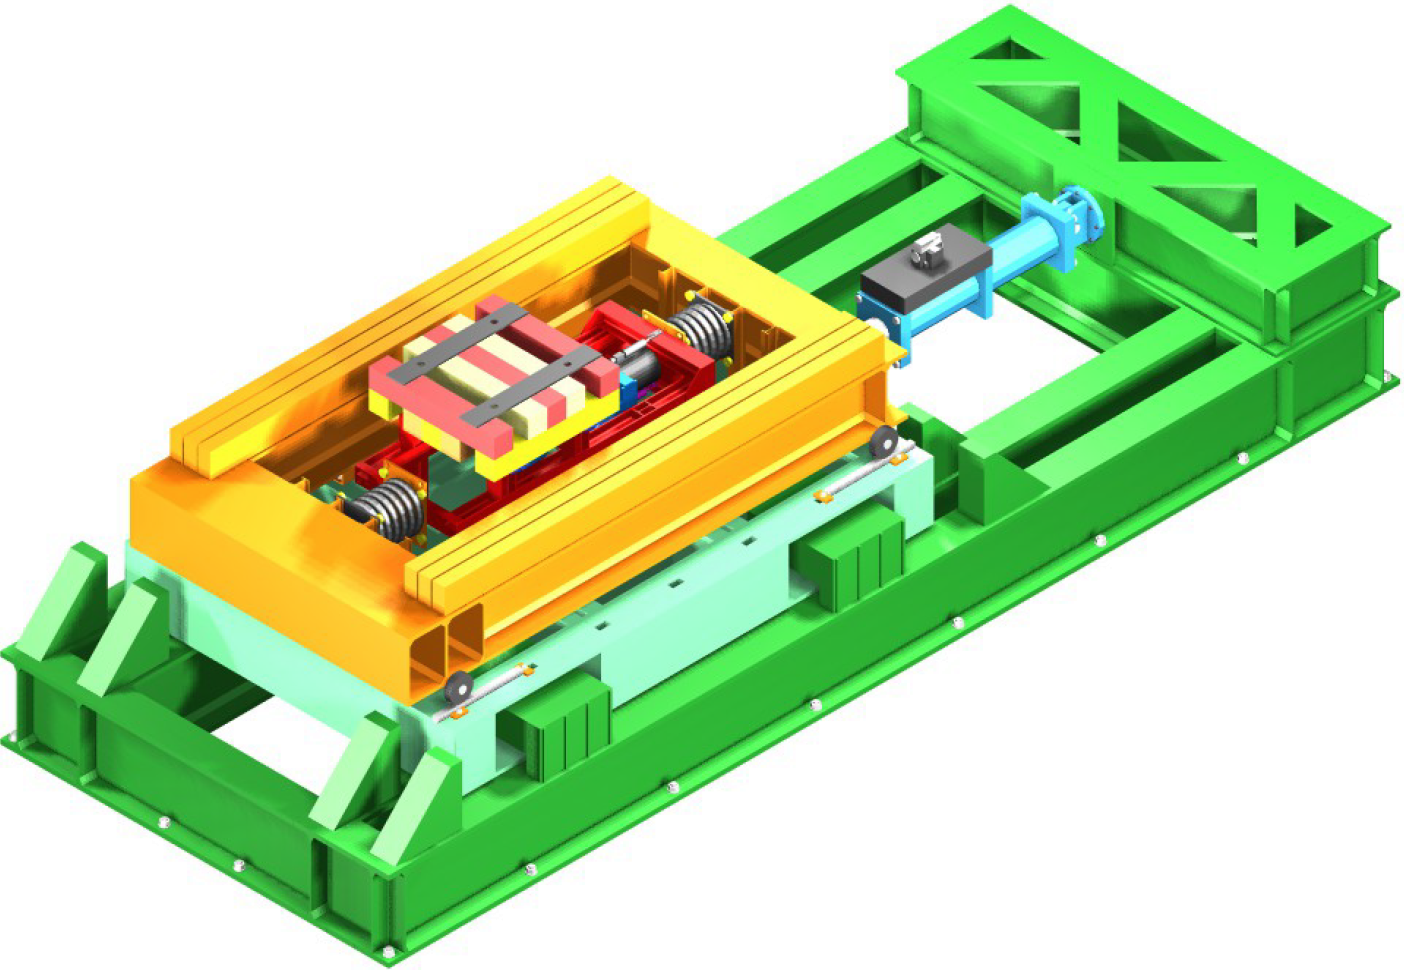
\includegraphics[width=\linewidth]{Figures/capa.png}
%     \caption{imagem do interior do shaker}
%     %\label{fig_sine_nonlinearity}
% \end{minipage}
% \hfill
% \begin{minipage}{0.49\textwidth}
%     \centering
%     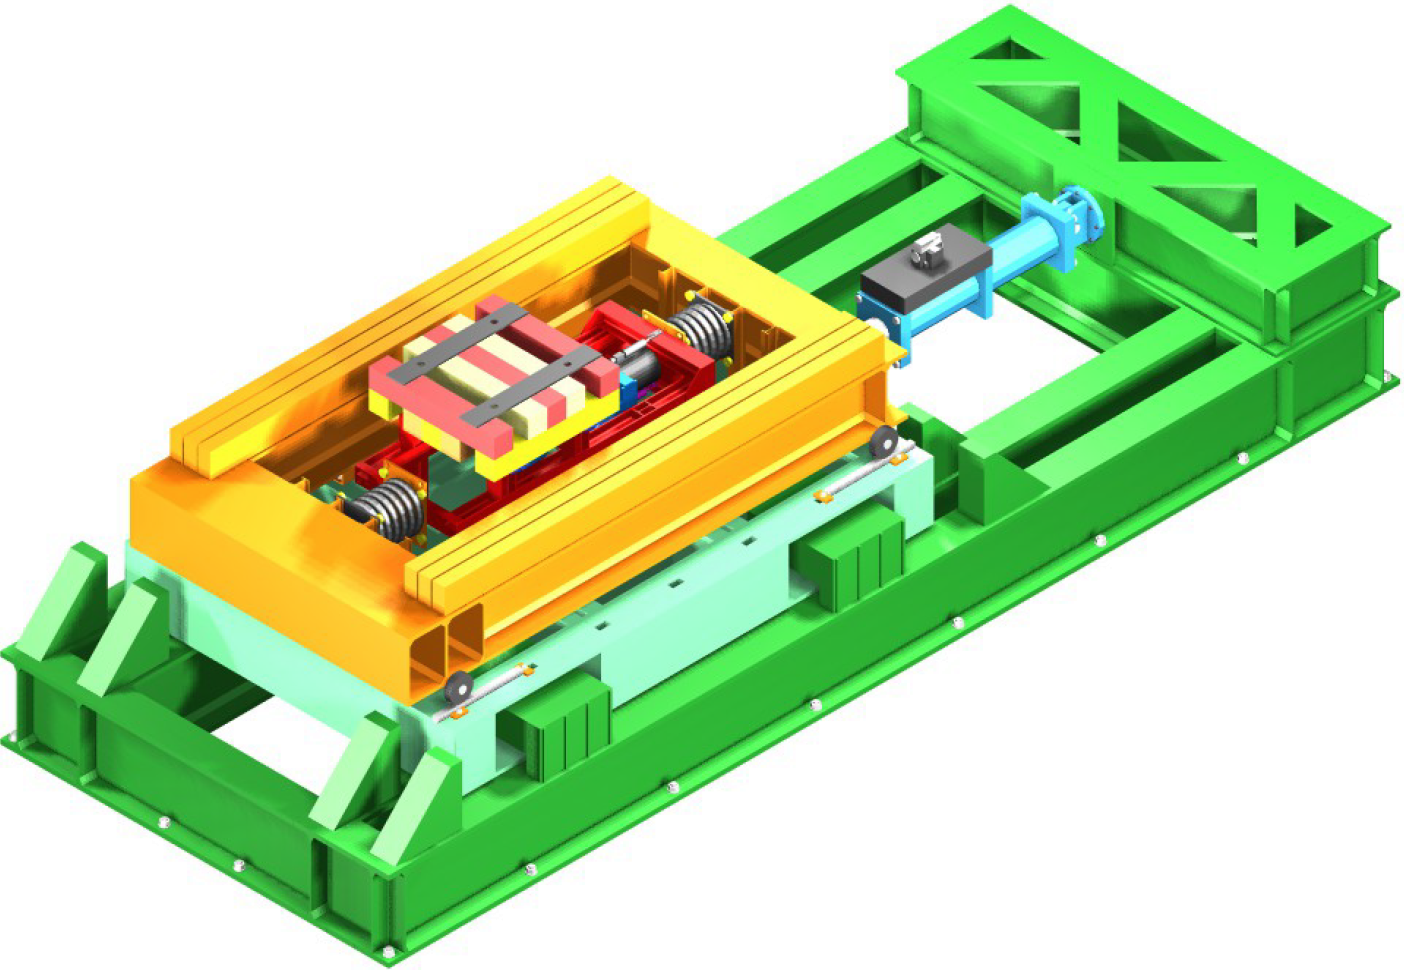
\includegraphics[width=\linewidth]{Figures/capa.png}
%     \caption{imagem das guias da mesa}
%     %\label{fig_square_nonlinearity}
% \end{minipage}
% \end{figure}

% Everything was reassembled together, and new data was collected for another system identification, however, a nonlinearity was still found.

% \section{ Implementar PID-F e controlo ótimo na aplicação de LabView de controlo das mesas}

% \begin{equation}
%     C(z) =  K_p + K_i \frac{T_s}{z-1} + K_d \frac{1}{T_f + \frac{T_s}{z-1}} 
% \end{equation}

\section{Results}

\subsection{System identification \& Controller Tuning}

The closed-loop frequency response obtained with each control method is shown on the Bode plot of figure \ref{Fig6_Shaking table control loop frequency response with controllers optimized for the Tolmezzo earthquake}

\begin{figure}[H]
    \centering
    
\includegraphics[scale=0.8]{experimental_validation/Bode_ClosedLoop.jpg}
    \caption{Shaking table control loop frequency response with controllers optimized for the Tolmezzo earthquake}
    \label{Fig6_Shaking table control loop frequency response with controllers optimized for the Tolmezzo earthquake}
\end{figure}

The frequency responses clearly highlights the benefits of optimizing the controllers (PID-F and LQI) since a larger bandwidth is obtained while maintaining a unitary gain at lower frequencies. This directly translates to improvements in the response spectrum, which will meet the target on the first run, instead of not requiring several iterations.

\subsection{Summary of Results}

The results obtained with the proposed methodology show how the tunning/optimization can improve significantly the performance of the system. It can be observed in \ref{Response spectra for a scaled-down Newhall fault parallel seismic signal} for acceleration and displacement response spectra of Tolmezzo earthquake, respectively, that the PID-F controller closely matches the target response, the LQI achieves an even closer match, whereas the OLI method (LNEC's approach) remains further from the target even after the third drive iteration. The MSE values quantify the differences observed among the curves.

\begin{figure}[H]
    \centering
    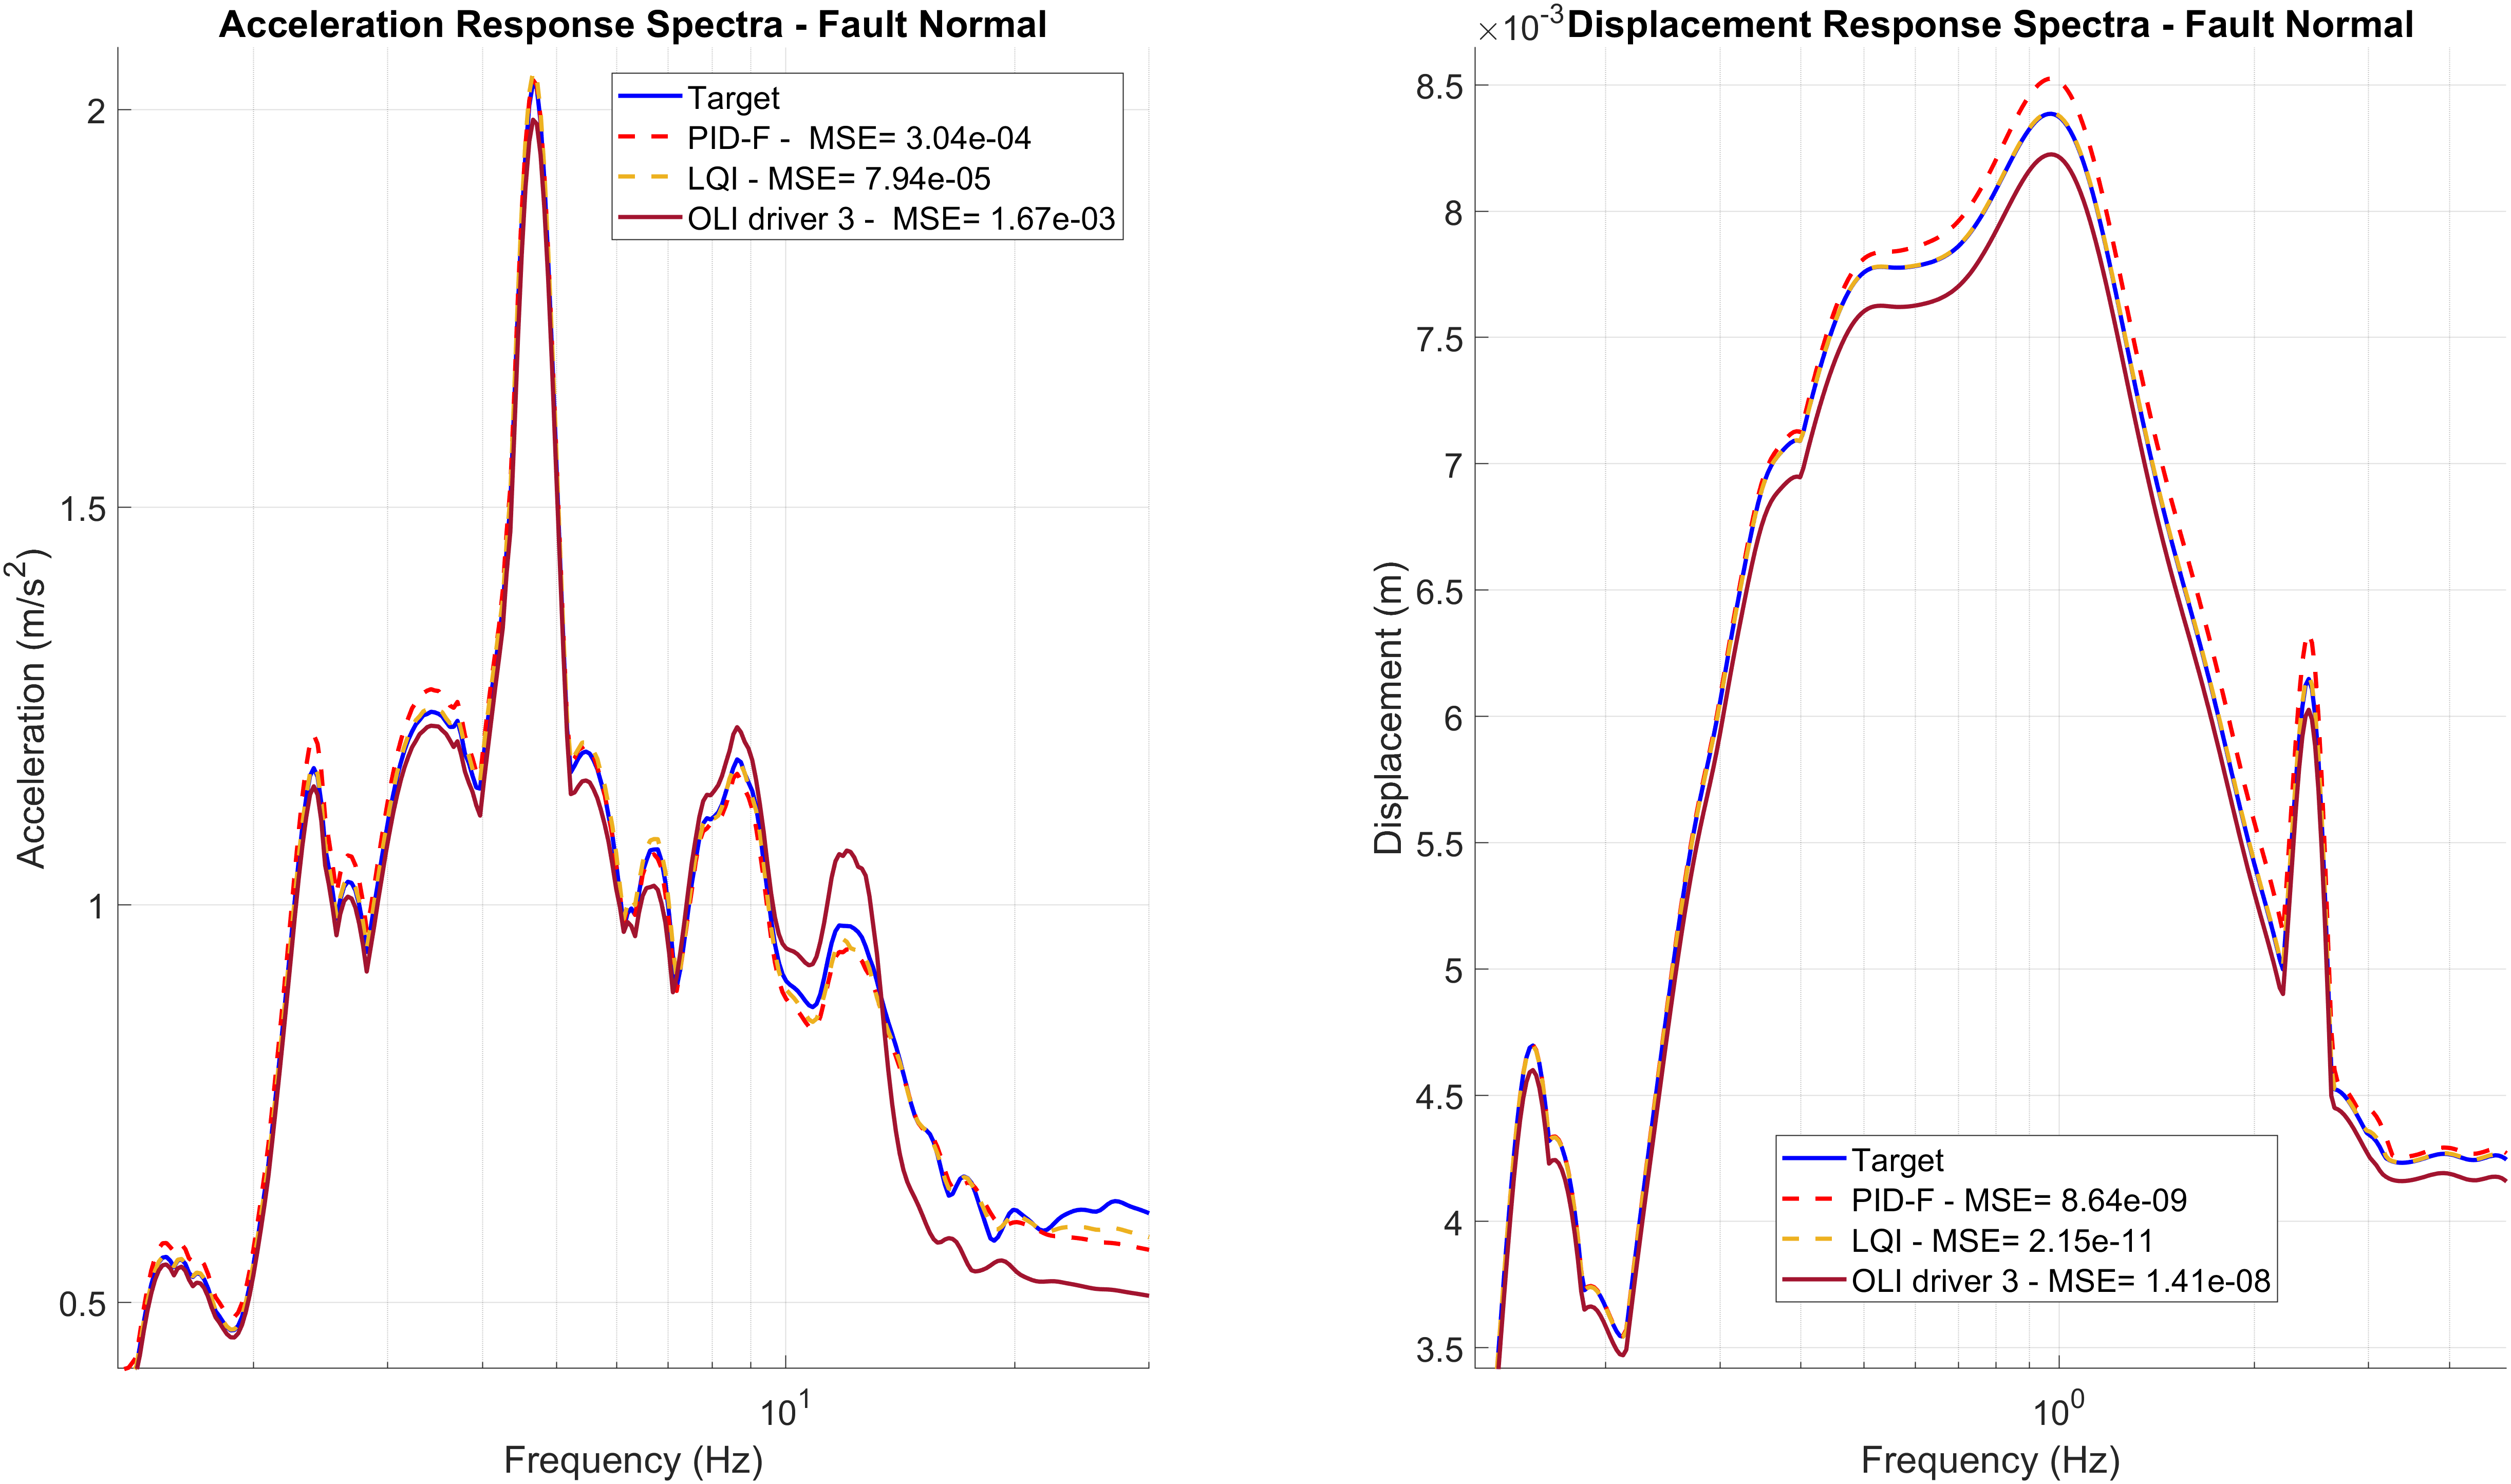
\includegraphics[width=\linewidth]{experimental_validation/Response_Spectra_Tolmezzo_results.png}
    \caption{Response spectra for a scaled-down Newhall fault parallel seismic signal}
    \label{Response spectra for a scaled-down Newhall fault parallel seismic signal}
\end{figure}

The results obtained for the remaining earthquakes exhibit the same trend, as shown in figures \ref{Acceleration response spectrum MSE for various seismic signals} and \ref{Displacement response spectrum MSE for various seismic signals}. This analysis confirms the benefits of using the proposed methodology, consistently identifying the LQI controller as the one that achieves the best closed-loop performance results.

\begin{figure}[H]
\begin{minipage}{0.49\textwidth}
        \centering
    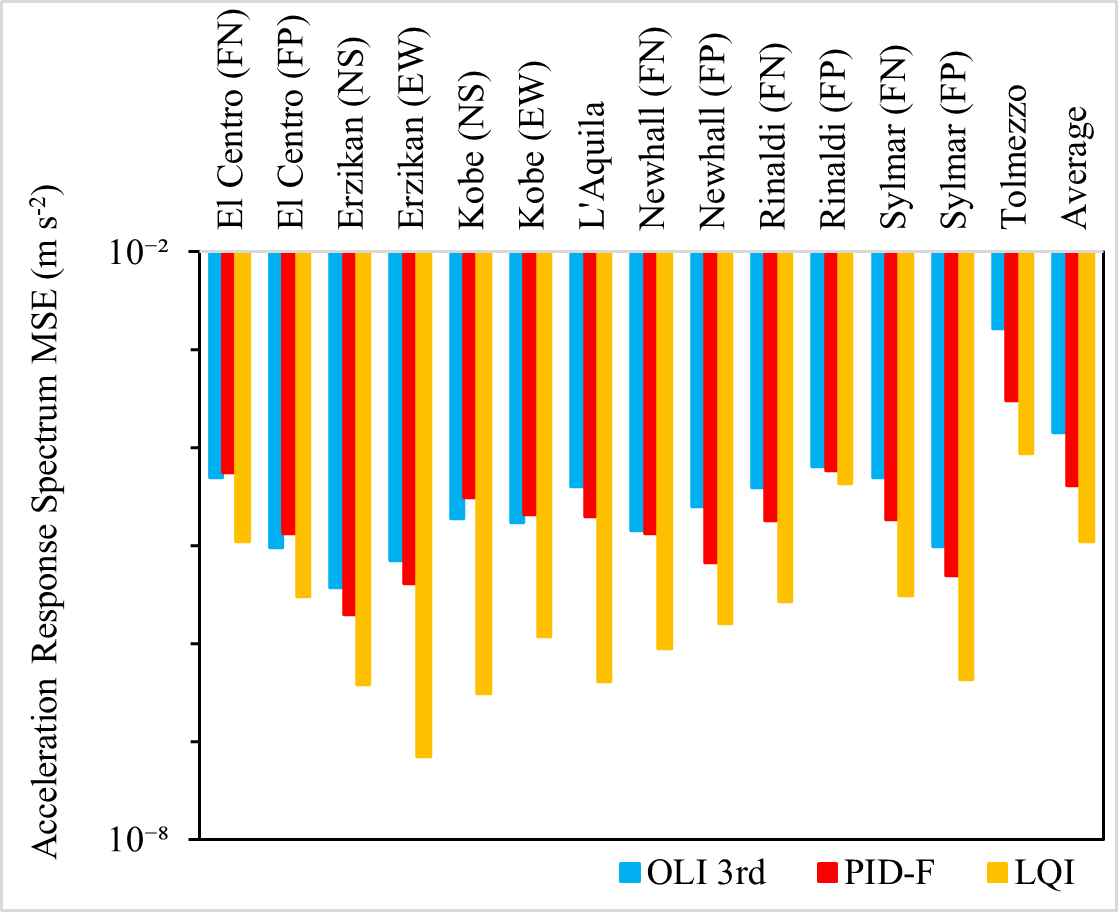
\includegraphics[width=\linewidth]{experimental_validation/BarChart_Accel.png}
    \caption{Acceleration response spectrum MSE for various seismic signals}
    \label{Acceleration response spectrum MSE for various seismic signals}
\end{minipage}
\hfill
\begin{minipage}{0.49\textwidth}
    \centering
    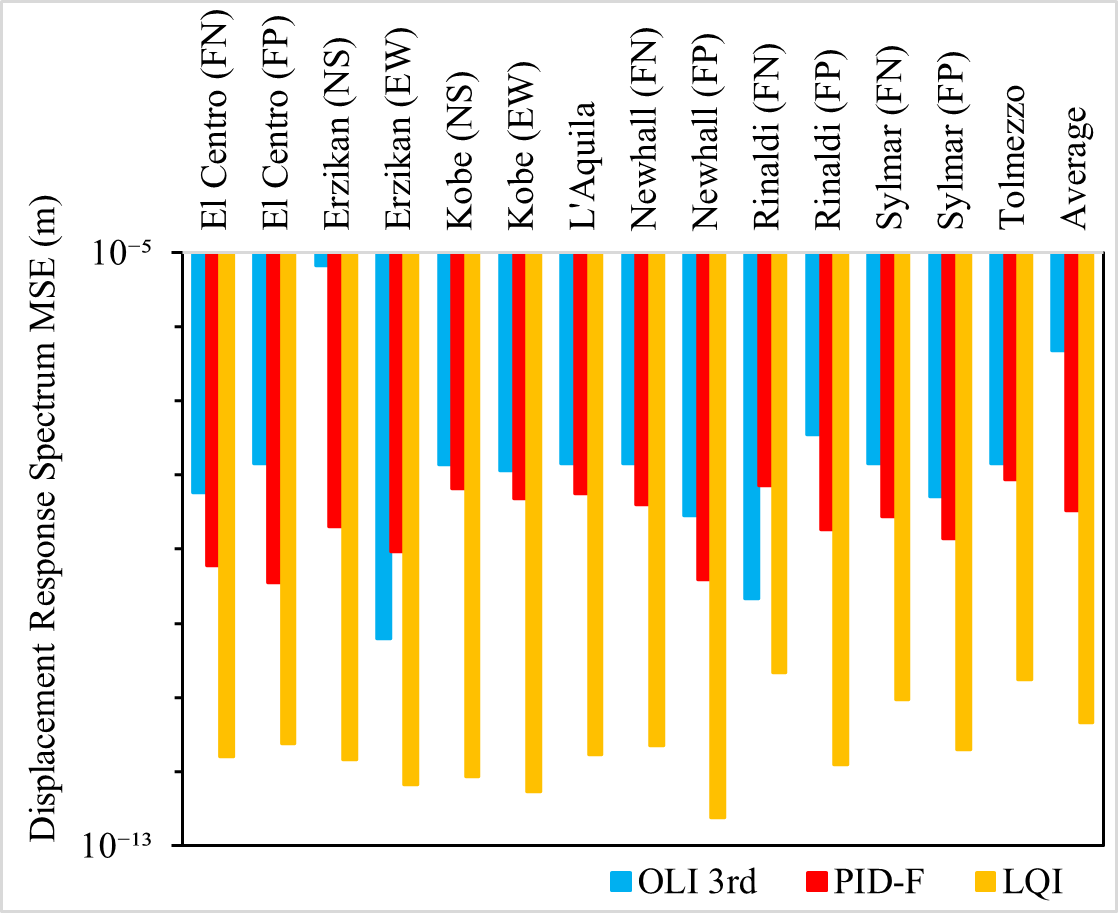
\includegraphics[width=\linewidth]{experimental_validation/BarChart_Disp.png}
    \caption{Displacement response spectrum MSE for various seismic signals}
    \label{Displacement response spectrum MSE for various seismic signals}
\end{minipage}
\end{figure}


\chapter{Conclusions \& Outlook}

This work presents an improved solution to the current OLI method used in LNEC to experimentally reproduce simulated earthquakes in laboratory shaking table setups. Based on model-based controllers and using the two-stage closed-loop identification method to identify the plant and  optimize the controllers, the PID-F and the LQI controllers were shown to reproduce the target response spectra across the whole frequency spectrum of the earthquake signal more accurately on the first run when compared with the standard OLI method fourth run. The tuned controllers (PID-F and LQI) also require less user intervention, and moreover, offer a systematic approach to the control problem with LQI controller providing the best results by significant margin for all earthquake ground-motions simulations.

Given the nature of shaking table experimental testing, the test specimens are often driven to plastic deformation, some form of failure, or have significant nonlinear behaviour which is not detectable in the small intensity identification experiments. This results in non-negligible shifts in dynamic properties and excitation of unknown modes that may occur during the test, and the proposed method of optimizing controllers for the plant dynamics cannot account for this, so further investment should be directed to the implementation of adaptive online identification methods that can inform nonlinear control strategies in order to address both the evolving and nonlinear test specimen dynamics.

The final step of the proposed methodology consists in implementing the optimized controllers on the physical system (small-scale shaking table). Completing this step will close the loop of the methodology and will enable the verification and confirmation of the results and the achieved performance. Subsequently, the methodology is intended to be implemented on LNEC's uniaxial shaking table, where the same analysis will be conducted to assess its effectiveness on larger-scale systems. This future stage aims to evaluate the scalability, robustness, and practical applicability of the proposed control strategy under more demanding testing conditions. After demonstrating their superior performance, the proposed methodology will be applied on future shaking table tests.


\clearpage
%% BIBLIOGRAFIA
\bibliographystyle{abbrvnat}
\setcitestyle{authoryear}
\bibliography{bibfile}

%%  APPENDIX
\appendix
\let\cleardoublepage\clearpage

\chapter{MTS Systems Control Strategies}\label{section:MTS_strategies}

\begin{figure}[H]
    \centering
    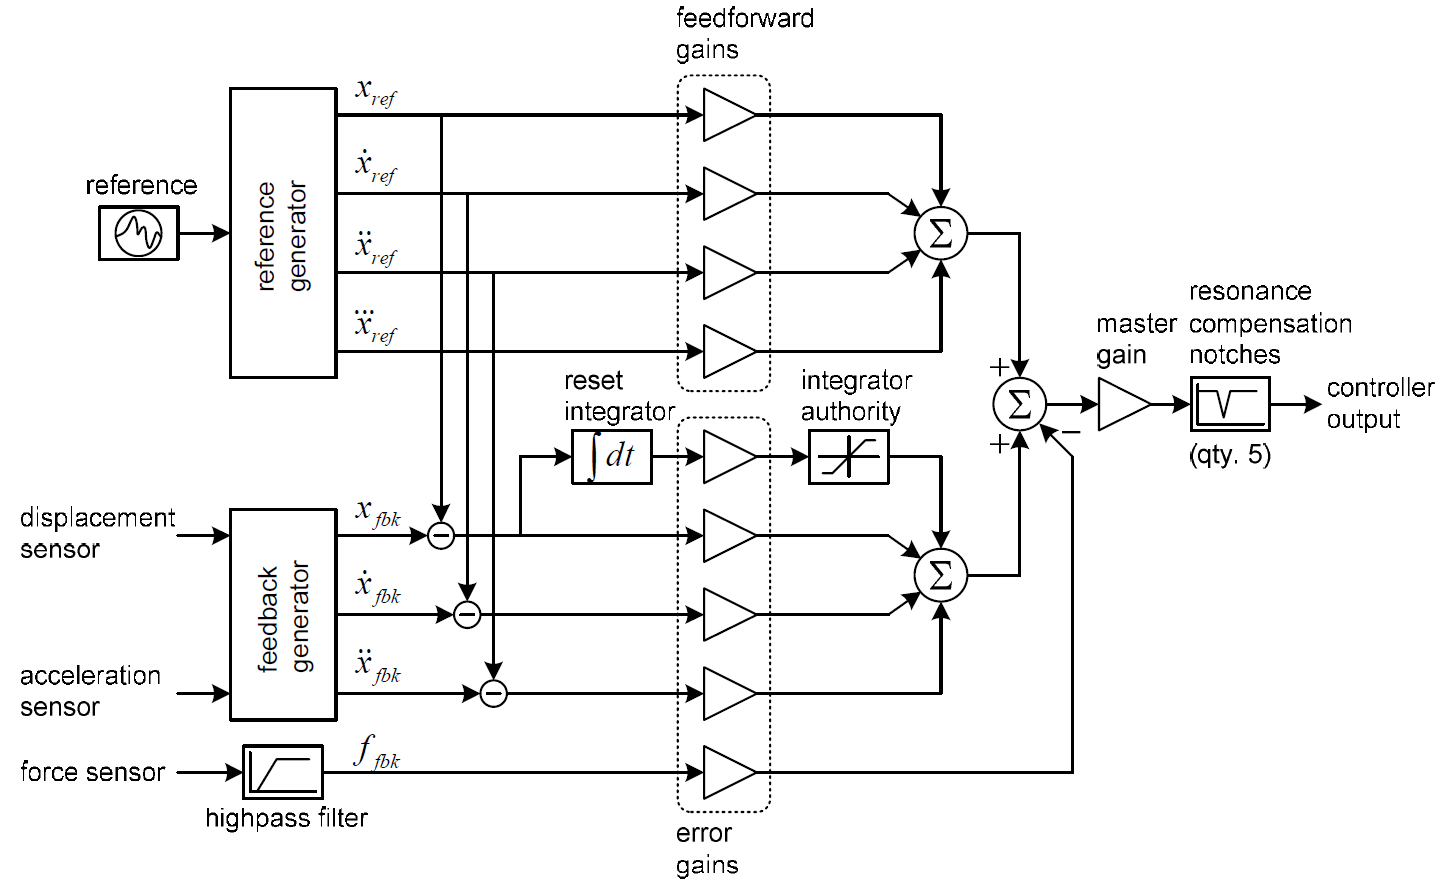
\includegraphics[width=\textwidth]{MTSsystems/tvc.png}
    \caption{Three-Variable Control (TVC)}
    \label{fig_TVC}
\end{figure}

\begin{figure}[H]
    \centering
\begin{subfigure}{\textwidth}
    \centering
    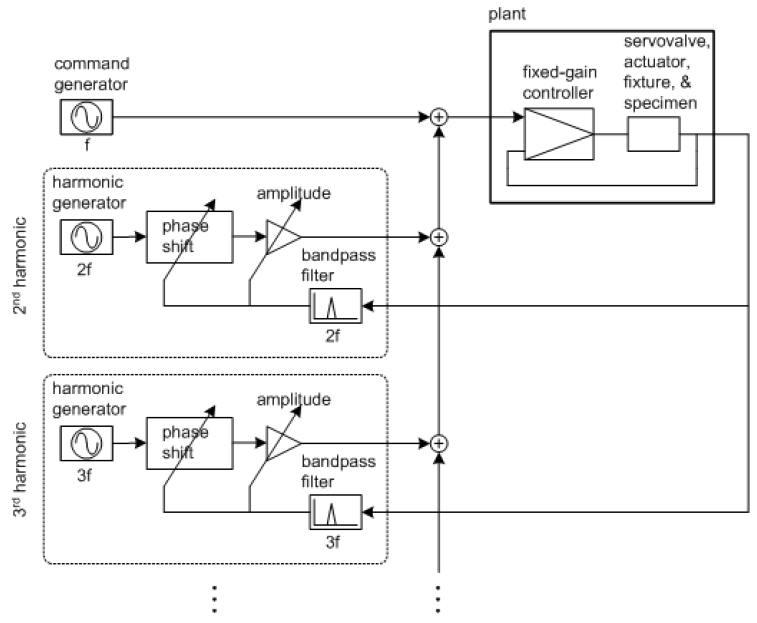
\includegraphics[width=0.7\textwidth]{MTSsystems/AHC.png}
    \caption{General representation}
\end{subfigure}
\\
\begin{subfigure}{\textwidth}
    \centering
    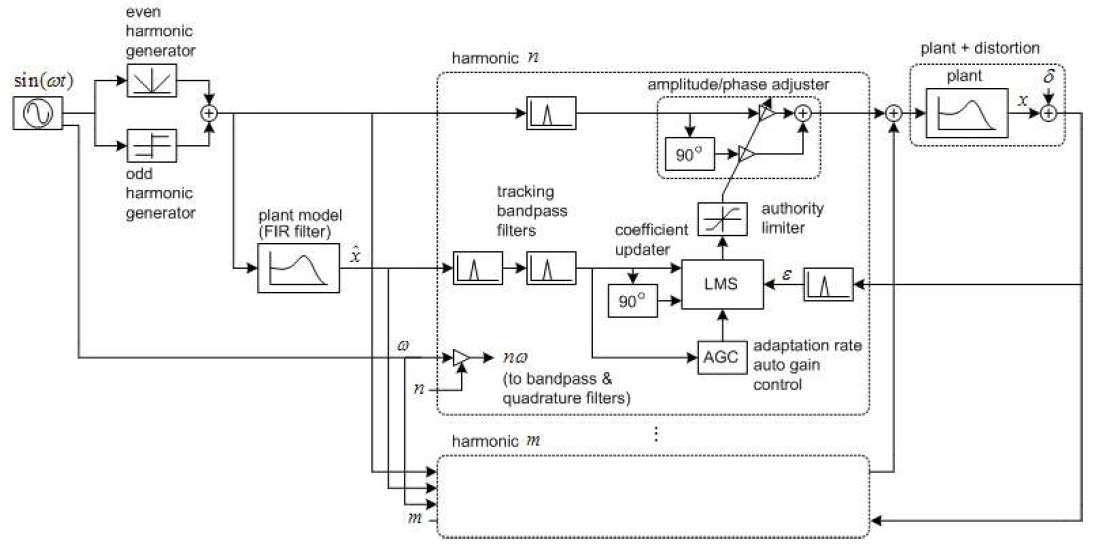
\includegraphics[width=\textwidth]{MTSsystems/AHC_detail.png}
    \caption{Detailed block diagram}
    \label{fig_AHC_detail}
\end{subfigure}
\caption{Adaptive Harmonic Cancellation (AHC)}
\label{fig_AHC}
\end{figure}

\begin{figure}[H]
    \centering
    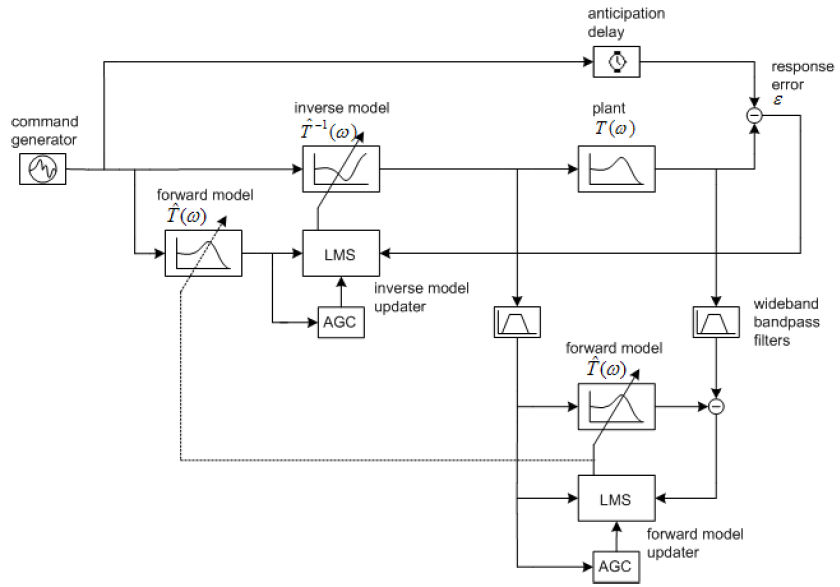
\includegraphics[width=0.95\textwidth]{MTSsystems/AIC.png}
    \caption{Adaptive Inverse Control (AIC)}
    \label{fig_AIC}
\end{figure}

\begin{figure}[H]
    \centering
    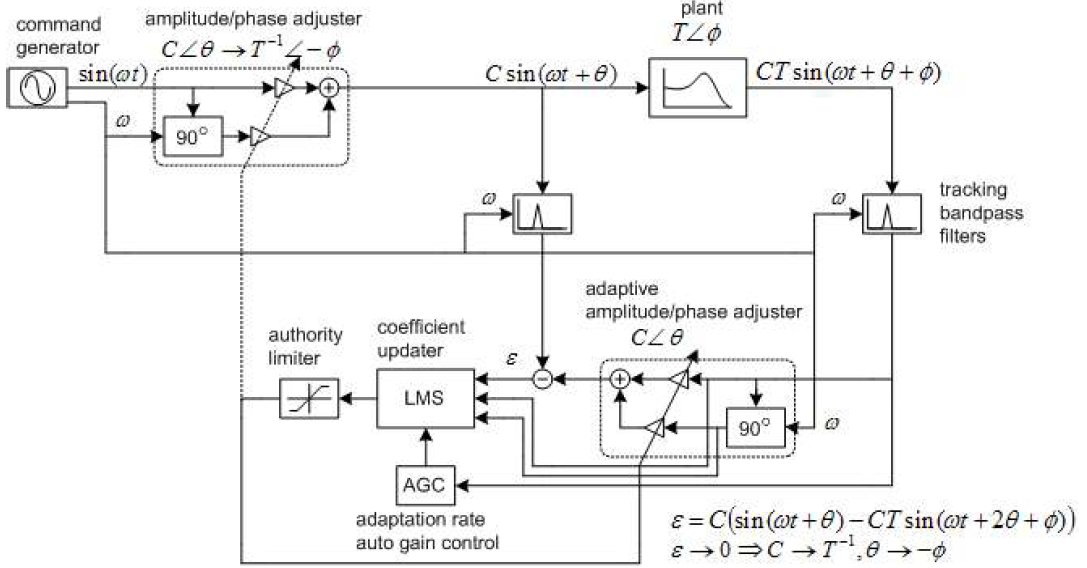
\includegraphics[width=\textwidth]{MTSsystems/APC.png}
    \caption{Amplitude/Phase Control (APC)}
    \label{fig_APC}
\end{figure}


\chapter{Tuned PID-F Performance Sensitivity to Test Specimen Parameters}\label{appendix:Tuned PID-F Performance Sensitivity to Test Specimen Parameters}


\begin{table}[H]
\centering
\caption{Parameter combinations and corresponding MSE values in figure \ref{Resp_Spectre_low_high_freq_and_damp}}
\begin{tabular}{cccccccc}
\hline
$f_1$ (Hz) & $f_2$ (Hz) & $\xi_1$ & $\xi_2$ & $i_{sv}$ (v) & $F_P$ (kN) & Accel. MSE ($m/s^2$) & Disp. MSE ($m$)\\ 
\hline
1.5 & 6.0  & 0.02 & 0.05 & 1.7 & 27 & $5.5\times10^{-2}$ &  $2.2\times10^{-6}$  \\
1.5 & 6.0  & 0.10 & 0.25 & 1.6 & 18 & $4.5\times10^{-3}$ &  $2.0\times10^{-6}$  \\
4.0 & 10.0 & 0.02 & 0.05 & 1.6 & 29 & $3.3\times10^{-2}$ &  $1.9\times10^{-6}$  \\
4.0 & 10.0 & 0.10 & 0.25 & 1.6 & 19 & $1.5\times10^{-2}$ &  $2.0\times10^{-6}$  \\
\hline
\end{tabular}
\label{tab:Resp_Spectre_low_high_freq_and_damp}
\end{table}

\begin{figure}[H]
    \centering
    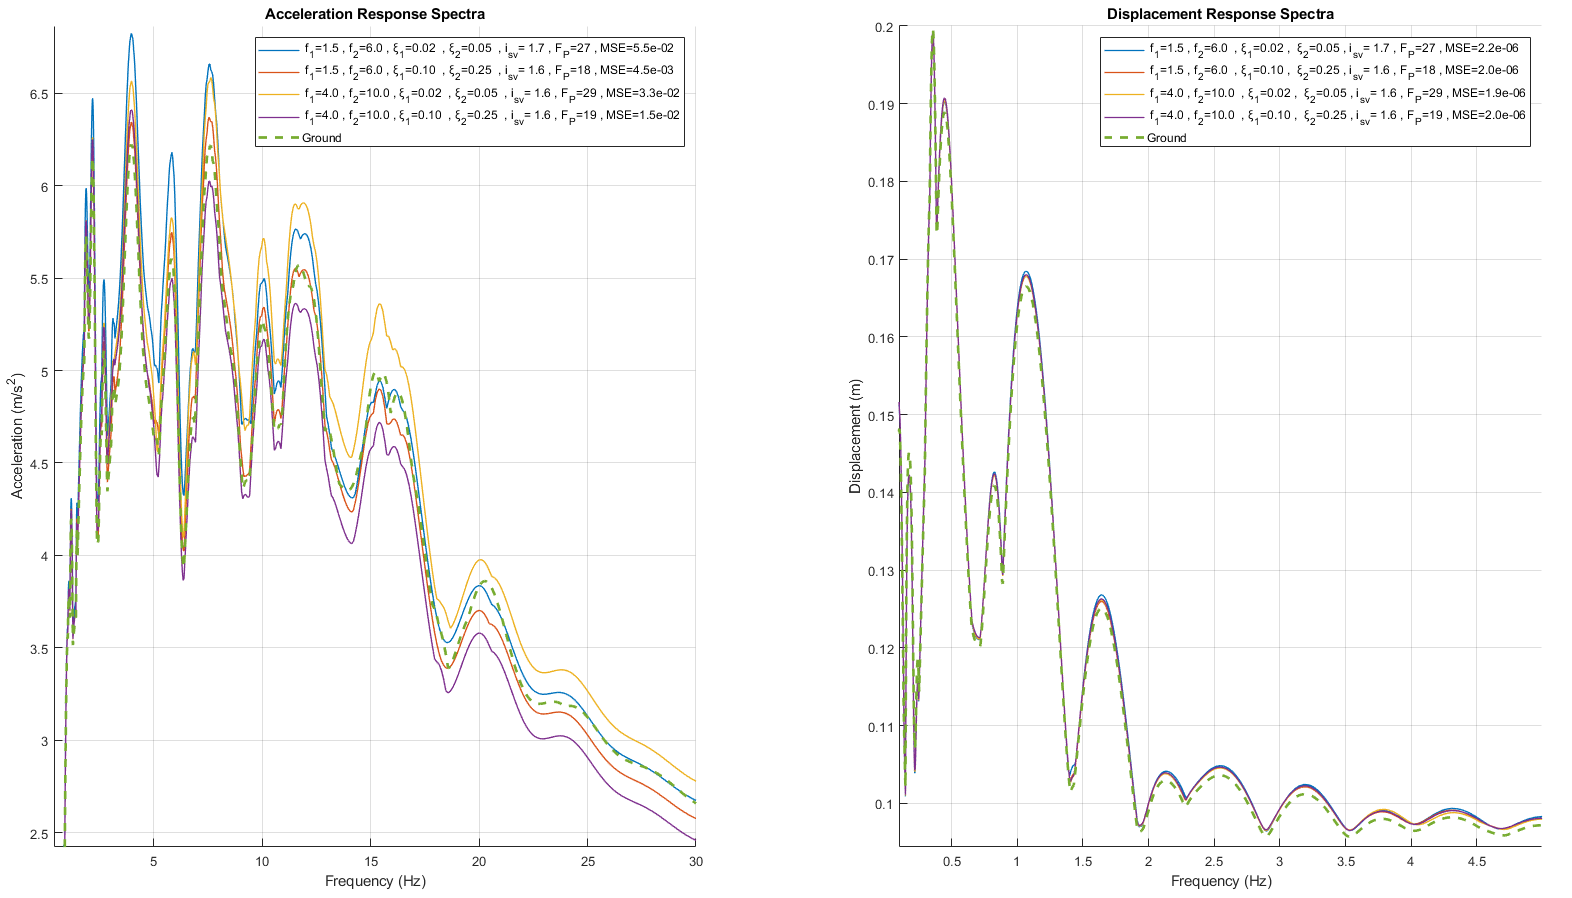
\includegraphics[width=1\linewidth]{MSE_Resp_Spectre/Resp_Spectre_low_high_freq_and_damp_cut.png}
    \caption{Response spectra for $m_1=m_2=2 \text{ ton}$, and different modal frequencies and damping}
    \label{Resp_Spectre_low_high_freq_and_damp}
\end{figure}

\pagebreak

\begin{table}[H]
\centering
\caption{Parameter combinations and corresponding MSE values in figure \ref{Resp_Spectre_f2_10}}
\begin{tabular}{cccccccc}
\hline
$f_1$ (Hz) & $f_2$ (Hz) & $\xi_1$ & $\xi_2$ & $i_{sv}$ (v) & $F_P$ (kN) & Acceleration MSE ($m/s^2$) & Displacement MSE ($m$)\\ 
\hline
1.5 & 10.0 & 0.02 & 0.05 & 1.7 & 28 & $6.0\times10^{-2}$ & $2.2\times10^{-6}$ \\
1.5 & 10.0 & 0.10 & 0.25 & 1.6 & 18 & $4.5\times10^{-3}$ & $2.0\times10^{-6}$ \\
4.0 & 10.0 & 0.02 & 0.05 & 1.6 & 29 & $3.3\times10^{-2}$ & $1.9\times10^{-6}$ \\
4.0 & 10.0 & 0.10 & 0.25 & 1.6 & 19 & $1.5\times10^{-2}$ & $2.0\times10^{-6}$ \\
\hline
\end{tabular}
\label{tab:Resp_Spectre_f2_10}
\end{table}

\begin{figure}[H]
    \centering
    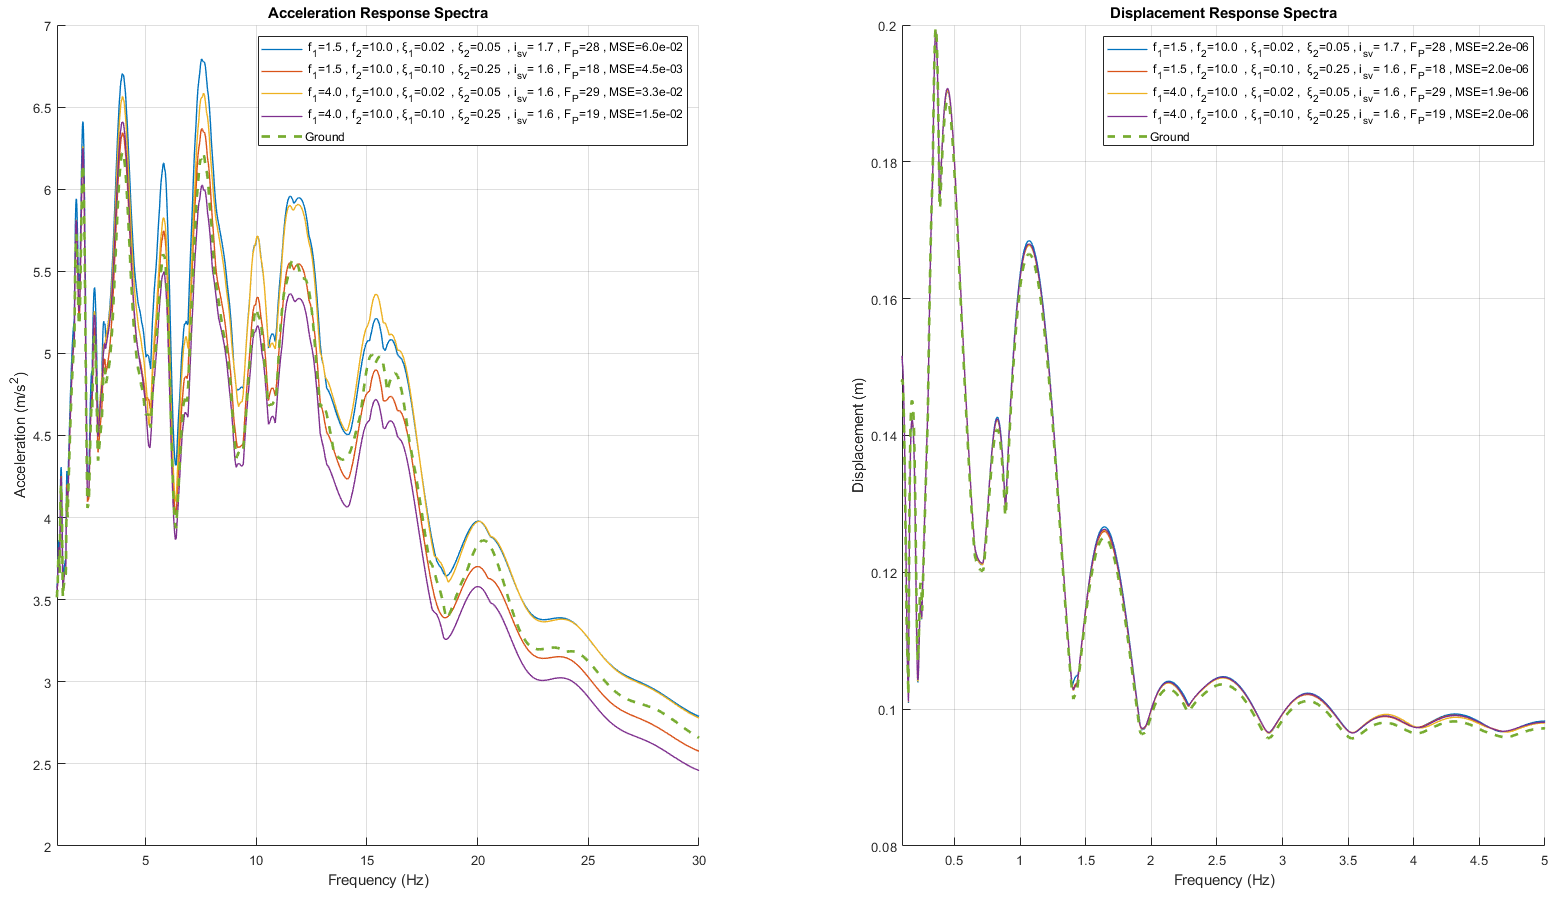
\includegraphics[width=1\linewidth]{MSE_Resp_Spectre/Resp_Spectre_f2=10_cut.png}
    \caption{Response spectra for $m_1=m_2=2\text{ ton}$, with $f_2=10$ Hz}
    \label{Resp_Spectre_f2_10}
\end{figure}

\pagebreak

\begin{table}[H]
\centering
\caption{Parameter combinations and corresponding MSE values in figure \ref{Resp_Spectre_f1_2415}}
\begin{tabular}{cccccccc}
\hline
$f_1$ (Hz) & $f_2$ (Hz) & $\xi_1$ & $\xi_2$ & $i_{sv}$ (v) & $F_P$ (kN) & Acceleration MSE ($m/s^2$) & Displacement MSE ($m$)\\ 
\hline
2.5 & 6.0  & 0.02 & 0.05 & 1.6 & 19 & $4.7\times10^{-3}$ & $2.0\times10^{-6}$ \\
2.5 & 6.0  & 0.10 & 0.25 & 1.6 & 16 & $1.1\times10^{-2}$ & $2.0\times10^{-6}$ \\
4.1 & 10.0 & 0.02 & 0.05 & 1.6 & 24 & $3.6\times10^{-2}$ & $1.8\times10^{-6}$ \\
4.1 & 10.0 & 0.10 & 0.25 & 1.6 & 16 & $1.5\times10^{-2}$ & $2.0\times10^{-6}$ \\
\hline
\end{tabular}
\label{tab:Resp_Spectre_f1_2415}
\end{table}

\begin{figure}[H]
    \centering
    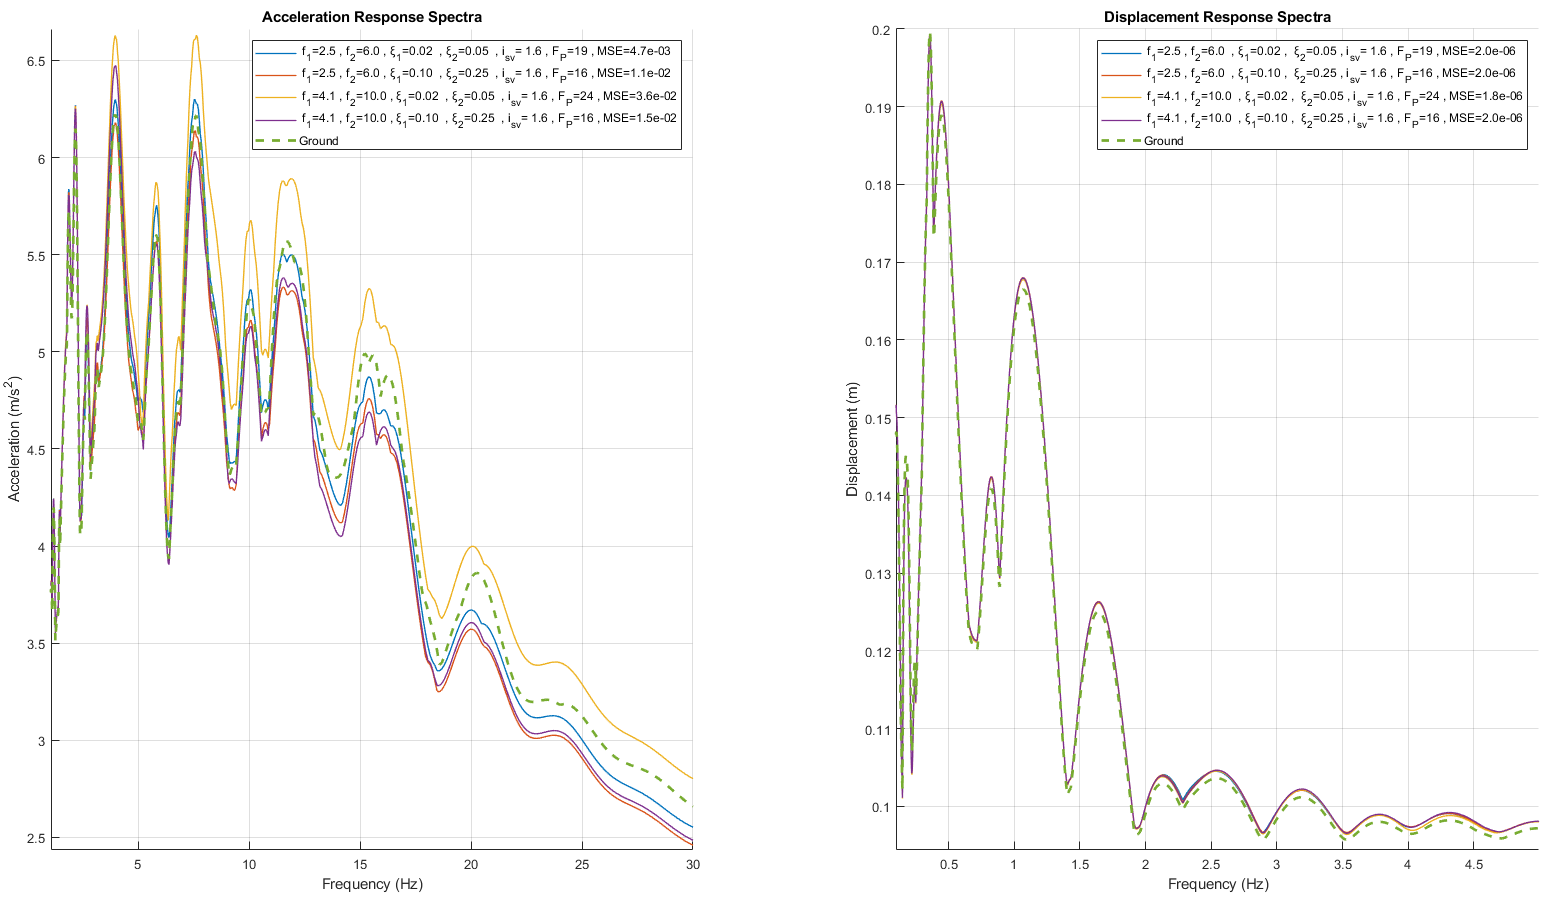
\includegraphics[width=1\linewidth]{MSE_Resp_Spectre/Resp_Spectre_f1_2415_cut.png}
    \caption{Response spectra for $m_1=m_2=2\text{ ton}$, and modal frequencies which are close together ($f_2 \approx2.415\cdot f_1$) (see figure \ref{fig_close_modal_freqs})}
    \label{Resp_Spectre_f1_2415}
\end{figure}

\begin{figure}
        \centering
    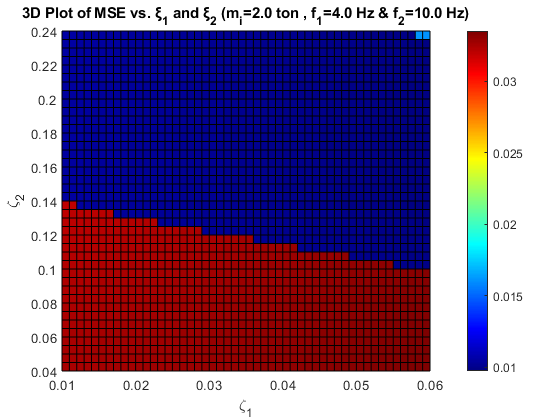
\includegraphics[width=0.6\linewidth]{MSE_Zeta/MSE vs Zeta (m_i=2.0,f_1=4.0, f_2=10.0)_old.png}
    \caption{Acceleration response spectra MSE vs damping ($\zeta_1$ and $\zeta_2$), with $m_1=m_2=2\text{ ton, }f_1=4 Hz, f_2=10 Hz$. }
    \label{fig_high_modal_freqs}
\end{figure}

\chapter{LQG Servo Controller Simulation Results}\label{appendix:LQG Servo_Controller_Simulation_Results}

\begin{figure}[H]
    \centering
    
\includegraphics[width=\linewidth]{LQG/Sim_Res_Qe9_tight/Response_Spectra.png}
    \caption{Response spectrum for fault normal. The response spectrum was obtained by sampling 500 frequencies logarithmically spaced between 0.1 and 30 Hz}%, and then applying a moving average filter with a window size of 25 points.}
    \label{fig_resp_spectrum_LQG_Qe9}
\end{figure}

\begin{figure}[H]
\begin{minipage}{0.49\textwidth}
    \centering
    
\includegraphics[width=\linewidth]{LQG/Sim_Res_Qe9_tight/Input_to_Servo.png}
    \caption{Input to servo}
    \label{fig_Input_to_Servo_LQG_Qe9}
\end{minipage}
\hfill
\begin{minipage}{0.49\textwidth}
    \centering
    
\includegraphics[width=\linewidth]{LQG/Sim_Res_Qe9_tight/Force_to_Platen.png}
    \caption{Force to Platen}
    \label{fig_Force_LQG_Qe9} 
\end{minipage}
\end{figure}
   
\begin{figure}[H]
\begin{minipage}{0.49\textwidth}
    \centering
    
\includegraphics[width=\linewidth]{LQG/Sim_Res_Qe9_tight/Platen_Acceleration.png}
    \caption{Platen acceleration}
    \label{fig_Platen_Acceleration_LQG_Qe9}
\end{minipage}
\hfill
\begin{minipage}{0.49\textwidth}
    \centering
    
\includegraphics[width=\linewidth]{LQG/Sim_Res_Qe9_tight/Platen_Displacement.png}
    \caption{Platen displacements}
    \label{fig_Platen_Displacement_LQG_Qe9}
\end{minipage}
\end{figure}

% \begin{figure}[H]
% \begin{minipage}{0.49\textwidth}
%     \centering
%     
\includegraphics[width=\linewidth]{LQG/Sim_Res_Qe9_tight/Platen_Acceleration_zoom.png}
%     \caption{Platen acceleration - Detailed view of the signals covering the period between 1.6 and 2.8 seconds}
%     \label{fig_Platen_Acceleration_zoom_LQG_Qe9}
% \end{minipage}
% \hfill
% \begin{minipage}{0.49\textwidth}
%     \centering
%     
\includegraphics[width=\linewidth]{LQG/Sim_Res_Qe9_tight/Platen_Displacement_zoom.png}
%     \caption{Platen displacements - Detailed view of the signals covering the period between 14.2 and 15.7 seconds}
%     \label{fig_Platen_Displacement_zoom_LQG_Qe9}
% \end{minipage}
% \end{figure}

\begin{figure}[H]
\begin{minipage}{0.49\textwidth}
    \centering
    
\includegraphics[width=\linewidth]{LQG/Sim_Res_Qe9_tight/Platen_Acceleration_Tracking_Error.png}
    \caption{Acceleration tracking error}
    \label{fig_Platen_Acceleration_Tracking_Error_LQG_Qe9}
\end{minipage}
\hfill
\begin{minipage}{0.49\textwidth}
    \centering
    
\includegraphics[width=\linewidth]{LQG/Sim_Res_Qe9_tight/Platen_Displacement_Tracking_Error.png}
    \caption{Displacement tracking error}
    \label{fig_Platen_Displacement_Tracking_Error_LQG_Qe9}
\end{minipage}
\end{figure}


\end{document}

% \chapter{Preliminary Conclusions \& Future Developments}
% \begin{itemize}
%     \item Both the displacement and acceleration tracking errors were significantly improved with the simple PID-F tune (Figures \ref{fig_response_spectrum_of_3}  to \ref{fig_Platen_Displacement_Tracking_Error}, table \ref{tab:mse_rs}).
%     \begin{itemize}
%     \item The cutoff frequency was increased from approximately 5 Hz to 18 Hz (Figure \ref{fig_Bode_of_G_xT_xref}) and response spectrum greatly improved (Figure \ref{fig_response_spectrum_of_3}).
%     \item A similar method could be simple to implement on the digital controller running on National Instruments hardware used at LNEC, and this may be an option worth exploring. In future work, different control strategies will also be explored.
%     \end{itemize}
%     \item It's important to note that these results are for both an outdated and simplified model:
%     \begin{itemize}
%         \item An identification of the seismic platform as it exists now, with the new hydraulic system, needs to be performed in the future.
%         \item Regarding the simplifications in this model, namely the fact that it does not account for any nonlinearities, nor was there any validation that the linearization assumptions are valid under the seen operating conditions, could be a problem, specially with the more aggressively tuned controller. 
%         \item Future  simulations needs to account for the nonlinearities in the system.
%         \item Another simplification, which will be accounted for in future work, is the fact that the controller in use at LNEC is digital, and thus discrete, and the simulations performed thus far did not account for discretization
%     \end{itemize}
% \end{itemize}

% \chapter{Possible modal frequencies for experimental setup on ST1D}
% The existing cart, with a mass of 1790 kg, and coil springs with stiffness of 17 kN/m (2 units) and 200 kN/m (4 units), allow coupling to the shaking table a 1-dof system with frequencies as high as 3.44 Hz, and as low as 0.41 Hz (with three 1100 kg masses added to the cart). Adding three 1100 kg masses to the cart setup with highest spring stiffness configuration results in a natural frequency of 2 Hz.
 
% \begin{align*}
% m &= 1790 kg \\
% k_{\text{list}} &= [17,\, 16.8,\, 201.1,\, 205.8,\, \approx200,\, \approx200] \ kN/m\\
% f_{\text{lowest}} &= \frac{1}{2\pi} \sqrt{\frac{17 + 16.8}{1790 + 3 \times 1100}} = 0.41 \\
% f_{\text{high K \&  mass}} &= \frac{1}{2\pi} \sqrt{\frac{17 + 16.8 + 201.1 + 205.8 + 200 + 200}{1790+ 3 \times 1100}} =  2.05
% \\
% f_{\text{highest}} &= \frac{1}{2\pi} \sqrt{\frac{17 + 16.8 + 201.1 + 205.8 + 200 + 200}{1790}} =  3.44 
% \end{align*}


% \clearpage
% \chapter{Proposed structure for the master's thesis}

% \section{Metodologia de Ensaios Sísmicos no LNEC}
% %Tempo estimado: 3 semanas;
% Compreender a metodologia de ensaios sísmicos utilizada no LNEC e desenvolver funções e modelos em Matlab/Simulink que reproduzam os ensaios em ambiente de simulação.

% \subsection{O modelo em anel fechado com controlador PID}
% Descrever e analisar o modelo do sistema em anel fechado utilizando um controlador PID.

% \subsection{Identificação dinâmica}
% Realizar a identificação dinâmica do sistema para caracterizar as suas propriedades dinâmicas.

% \subsection{Geração do sinal de comando}
% Desenvolver e avaliar algoritmos para a geração do sinal de comando.

% \subsection{Construção do espectro de resposta}
% Construir o espectro de resposta do sistema e utilizá-lo para análise de desempenho.

% \subsection{Análise do método como um todo}
% Realizar uma avaliação abrangente da metodologia adotada.

% \subsection{Análise do sistema com o modelo matemático construído}
% Utilizar métodos analíticos como Lugar das Raízes (LGR) ou diagramas de Bode para estudar o comportamento do sistema baseado no modelo matemático desenvolvido.

% \subsection{Avaliação do comportamento sob ações sísmicas}
% Examinar o desempenho do sistema perante ações sísmicas e identificar as suas vantagens e limitações.

% \subsection{Avaliação do método de geração do sinal de comando}
% Avaliar a eficácia e eficiência do método de geração do sinal de comando.

% \subsection{Resumo do Método de Ensaio no LNEC}
% Os ensaios realizados no LNEC visam avaliar a vulnerabilidade estrutural, verificando a evolução dos danos com o aumento da severidade sísmica. A metodologia consiste nos seguintes passos:

% \begin{enumerate}
%     \item \textbf{Definição do sinal sísmico de referência:} Estabelecer o sinal de referência (deslocamento, velocidade e aceleração).
%     \item \textbf{Identificação do sistema:} Determinar a Função de Resposta em Frequência (FRF) do sistema plataforma + modelo.
%     \item \textbf{Geração do sinal de comando:} Criar o sinal de Drive utilizando o método \textit{Online Iteration}, com base no sinal de referência e no modelo identificado.
%     \item \textbf{Execução do ensaio sísmico:} Aplicar o sinal de comando ao sistema em anel fechado.
%     \item \textbf{Avaliação do desempenho:} Comparar os espectros de resposta do sinal medido e do sinal de referência.
%     \item \textbf{Iteração ou término:} Repetir o procedimento para maior amplitude ou encerrar a campanha se o último nível for atingido.
% \end{enumerate}


% \section{Instalação Experimental}
% %Tempo estimado: 5 semanas;
% Concluir a instalação da plataforma sísmica ST1D, incluindo os sistemas hidráulico e de automação. Compreender o funcionamento do sistema de medição e controlo, que utiliza equipamento National Instruments e programação em LabView. Implementar e analisar o controlador PID em cascata com retroação de deslocamento e força.

% \section{Formação em LabView}
% %Tempo estimado: 2 semanas;
% Participar na formação organizada pelo LNEC para desenvolver competências em LabView, necessárias para a posterior implementação do controlador otimizado na plataforma ST1D.

% \section{Validação Experimental do Sistema}
% %Tempo estimado: 6 semanas;
% Realizar os ensaios experimentais para validar os modelos desenvolvidos e o funcionamento da plataforma sísmica ST1D.

% \subsection{Configuração dos Ensaios}
% Configurar a plataforma com base nos requisitos previamente definidos, incluindo a definição de parâmetros como amplitude, frequência e tipo de entrada para o controlador.

% \section{Definição da Instrumentação e Calibração do Sistema}
% %Tempo estimado: 3 semanas;
% Proceder à definição da instrumentação a utilizar nos ensaios, calibrar os sensores com recurso a padrões de referência metrológicos, e parametrizar curvas de calibração na aplicação para operação e controlo da plataforma sísmica;


% \subsection{Ensaios de Validação do Modelo 1-DOF}
% Realizar testes experimentais utilizando o modelo 1-DOF e comparar os resultados obtidos com os previstos pelos modelos matemáticos desenvolvidos em Matlab/Simulink.

% \subsection{Ensaios de Validação do Modelo 2-DOF}
% Reproduzir cenários dinâmicos mais complexos com o modelo 2-DOF e analisar o desempenho da plataforma e a precisão do modelo em prever a resposta estrutural.

% \subsection{Avaliação do Desempenho do Controlador PID}
% Estudar o comportamento do sistema com o controlador PID implementado, comparando as respostas esperadas e observadas em condições reais.

% \subsection{Testes com Diferentes Tipos de Sinais}
% Avaliar a resposta da plataforma com diferentes tipos de entradas, incluindo sinais harmónicos, aleatórios e sinais sísmicos reais.

% \subsection{Geração do Espectro de Resposta Experimental}
% Obter o espectro de resposta experimental e comparar com os resultados teóricos e de simulação, analisando discrepâncias e ajustando os modelos conforme necessário.

% \section{Relatório Final e Apresentação}
% %Tempo estimado: 3 semanas;
% Elaborar o relatório final e preparar a apresentação do trabalho desenvolvido.

% \subsection{Elaboração do Relatório Final}
% Preparar um documento detalhado que inclua:
% \begin{itemize}
%     \item Descrição do trabalho realizado e do progresso alcançado;
%     \item Modelos matemáticos desenvolvidos e resultados das simulações;
%     \item Metodologia de ensaios sísmicos implementada;
%     \item Validação experimental e análise de resultados;
%     \item Identificação de limitações e propostas de trabalhos futuros.
% \end{itemize}

% \subsection{Apresentação dos Resultados}
% Preparar uma apresentação que resuma o trabalho e destaque as principais conclusões, destinada a um público técnico e/ou académico.

% % \chapter{Cronograma}
% % %Tempo estimado: Variável; depende das fases e iterações.
% % Organizar um cronograma detalhado para cada uma das atividades, com prazos claros e estimativas de duração para o cumprimento das etapas do projeto.

% % \chapter{Conclusão}
% % O presente plano visa o desenvolvimento completo de modelos matemáticos e experimentais para a plataforma sísmica ST1D, incluindo a implementação de sistemas de controlo, simulações e validações experimentais. O cumprimento deste plano contribuirá para o avanço no estudo de resposta dinâmica de estruturas sob ações sísmicas, bem como para o aprimoramento da metodologia de ensaios do LNEC.










% %%%%%%%%%%%%%%%%%%%%%%%%%%%%%%%%%%%%%%%%%%%%%%%%%%%%%%%%%%%%%%%%%%%%%%%%%%%%%%%%%%%%%%%%%%%%%%%%%%%
% %%%%%%%%%%%%%%%%%%%%%%%%%%%%%%%%%%%%%%%%%%%%%%%%%%%%%%%%%%%%%%%%%%%%%%%%%%%%%%%%%%%%%%%%%%%%%%%%%%%

% %%% THIS CODE FITS 2 IMAGES SIDE BY SIDE
% % \begin{figure}[H]
% % 
% % \begin{minipage}{0.30\textwidth}
% % \centering
% %     \includegraphics[width=\textwidth]{Figures/226_input_force.jpg}
% %     \caption{$F_3$ over time.}
% %     \label{fig:ex7_input_force}
% % \end{minipage}
% % \hfill
% % \begin{minipage}{0.30\textwidth}
% %     \centering
% %     \includegraphics[width=\textwidth]{Figures/226_input_torque.jpg}
% %     \caption{$M_1$,  $M_2$ and  $M_3$ over time.}
% %     \label{fig:ex7_input_torque}
% % \end{minipage}
% % 
% % \end{figure}


% %%% THIS CODE FITS 3 IMAGES SIDE BY SIDE

% % \begin{figure}[H]
% % \begin{minipage}{0.30\textwidth}
% %     \includegraphics[width=\textwidth]{Figures/226_accel.jpg}
% %     \caption{Acceleration over time.}
% %     \label{fig:ex7_accel}
% % \end{minipage}
% % \hfill
% % \begin{minipage}{0.30\textwidth}
% %     \includegraphics[width=\textwidth]{Figures/226_vel.jpg}
% %     \caption{Velocity over time.}
% %     \label{fig:ex7_vel}
% % \end{minipage}
% % \hfill
% % \begin{minipage}{0.30\textwidth}
% %     \includegraphics[width=\textwidth]{Figures/226_pos.jpg}
% %     \caption{Position over time.}
% %         \label{fig:ex7_pos}
% % \end{minipage}
% % \end{figure}




% %%%%%%%%%%%% TRASH CAN %%%%%%%%%%%%

% \chapter{Definição do Problema}
% O atual processo para realização de ensaios em plataforma sísmica no LNEC compreende a sintetização \textit{offline} de um sinal de comando (Drive) diferente da referência por forma a que a plataforma vibre de acordo com o sinal de referência, i.e., o sismo (Ref.). O sistema plataforma sísmica mais estrutura a testar tem implementado um controlador PI - Proporcional Integral, com parâmetros fixos. 

% No ensaio sísmico, a estrutura é exposta a um conjunto de testes com amplitudes do sismo diferentes, i.e., inicialmente é testada com o sismo a uma amplitude reduzida, sendo depois avaliados os danos. De seguida, com o mesmo sismo a uma amplitude maior, são novamente avaliados os danos, e assim sucessivamente até uma amplitude definida, que normalmente é a amplitude do sismo original. 

% Antes de cada teste é efetuada uma identificação dinâmica do sistema utilizando um sinal de Ruído Branco de Banda Limitada (sempre com a mesma amplitude) para obtenção da Função de Transferência do Sistema, que é utilizada no algoritmo para gerar o sinal de comando. Ao longo deste processo, a amplitude do sinal de referência é aumentada de teste para teste e é de esperar que a estrutura atinja um regime não linear, quer devido ao comportamento de eventuais componentes de que dispõe, quer resultante do dano acumulado na estrutura ao longo dos vários testes. 

% No final de cada teste, o desempenho do sistema é avaliado pela comparação do espectro de resposta do sinal de referência com o do sinal medido na plataforma. Um bom desempenho ou mesmo um desempenho razoável nem sempre é conseguido com o sinal de comando sintetizado, sendo por vezes necessário gerar mais do que um sinal de comando e, consequentemente, realizar mais do que um ensaio à mesma amplitude, o que seria preferível evitar visto que introduz dano na estrutura. 

% A par disto, existe ainda a limitação física do equipamento, que se traduz na prática na limitação finita do campo de deslocamento, velocidade e aceleração, que devem ser contabilizados.

% \chapter{Definição de Objetivos}
% Implementar o melhor controlador (ou estratégia) que garanta que as vibrações da plataforma seguem exatamente o sinal sísmico de teste (referência/sismo), tendo em conta que:
% \begin{itemize}
%     \item A amplitude do sismo aumenta de teste para teste na mesma campanha de ensaio;
%     \item Antes de cada teste é feita uma identificação dinâmica a amplitude baixa (para não danificar o modelo); será possível utilizar a resposta do sismo para identificar o modelo, ou complementar o modelo identificado para amplitudes mais altas?;
%     \item O sinal de comando gerado \textit{offline} é imposto na plataforma sísmica sem se verificar se permite obter um bom desempenho por simulação;
%     \item O sistema plataforma sísmica ST1D (1DOF) pode testar modelos até $m = 5t$, tem uma banda de interesse $0 \leq f (\mathrm{Hz}) \leq 25$ com limitações em termos de deslocamento $-100 \leq d (\mathrm{mm}) \leq +100$, velocidade $-40 \leq v (\mathrm{cm/s}) \leq +40$, e aceleração $-25 \leq a (\mathrm{m/s^2}) \leq +25$; estas características terão de ser verificadas aquando dos ensaios laboratoriais;
%     \item O modelo a ensaiar pode inicialmente ter ou não um comportamento linear, mas à medida que fica danificado é de certeza não linear; as estruturas a testar têm em geral 2 modos de vibração na banda de interesse da plataforma sísmica: $1.5 \leq f_1 (\mathrm{Hz}) \leq 4$, $2 \leq \xi_1 (\%) \leq 5$, $6 \leq f_2 (\mathrm{Hz}) \leq 10$, $5 \leq \xi_2 (\%) \leq 15$, para estrutura sem dano (no início do ensaio, i.e., primeiro teste), onde o amortecimento pode chegar a $\xi_1 = 10\%$ e $\xi_2 = 25\%$ para a estrutura com dano;
%     \item O desempenho é avaliado por comparação do espectro de resposta da referência com o do sinal medido.
% \end{itemize}


% \chapter{Revisão do Estado da Arte}
% %Tempo estimado: 2 semanas e, realizar ao longo do trabalho sempre que se julgue necessário;
% Pesquisa de referências sobre as técnicas para ensaios sísmicos e em particular sobre os ensaios em plataforma sísmica, incluindo os métodos de ensaio, configurações de montagem, bem como a instrumentação para medição e controlo dos equipamentos;




% \chapter{Modelação Matemática}
% %Tempo estimado: 2 semanas;
% Estes modelos devem ser programados Matlab/Simulink; devem ser preparadas funções/scripts/interfaces que permitam facilmente parametrizar o modelo, calcular propriedades (modos de vibração), analisar e simular para várias entradas (sonda sinusoidal, onda quadrada, input externo – sismo);


% \section{Modelo 1-DOF}
% Pesquisa geral de modelos ou classe de modelos matemáticos para reproduzir o comportamento dinâmico de plataformas sísmicas acionadas por unidades óleo-hidráulicas, compreender o equipamento plataforma sísmica ST1D e modelar os componentes principais que contribuem para o seu comportamento dinâmico;

% % 1DOF model
% $H_{1DoF} = \frac{-m_{sp} s^2}{m_{sp} s^2 + c_{sp} s + k_{sp}}$

% \vspace{4mm}

% $m_t = m_p + m_{sp} \left( 1 + H_{sp} \right)$
% \vspace{4mm}
% % m_t = m_p + m_{sp}      % rigid mass


% $G_{xr} = \frac{10^{-4} A k_h k_p k_s v_k q}{10^{-4} A k_h k_p k_s v_k q + s \left( s \tau_{sv} + 1 \right) \left( A^2 c_{tm} s + A^2 k_h + A^2 m_t s^2 + k_{pl} c_{tm} k_h + k_{pl} k_h m_t s \right)}$
% \vspace{4mm}

% % FT do anel aberto G_{aa} = \frac{x_p}{i_{sv}}
% $G_{ol} = \frac{x_p}{i_{sv}}= \frac{10^{-4} A k_h k_s v_k q}{s \left( s \tau_{sv} + 1 \right) \left( A^2 c_{tm} s + A^2 k_h + A^2 m_t s^2 + k_{pl} c_{tm} k_h + k_{pl} k_h m_t s \right)}$
% \vspace{4mm}

% % FT do anel fechado
% $G_{cl} = \frac{G_{ol}\cdot k_p}{1 + G_{ol}\cdot k_p}$

% \section{Modelo 2-DOF}
% Definição do modelo 2DOF massa/mola/amortecedor da estrutura a associar à plataforma que simula a estrutura a testar, tendo em conta as características definidas e, considerar a possibilidade de introduzir não-linearidades;



% \chapter{Metodologia de Ensaios Sísmicos no LNEC}
% %Tempo estimado: 3 semanas;
% Compreender o método de ensaios sísmicos LNEC e construir as funções/modelos em Matlab/Simulink que permitam reproduzir o ensaio em ambiente de simulação, nomeadamente:

% \section{O modelo em anel fechado do sistema com um controlador PID}
% Descrever e analisar o modelo em anel fechado do sistema utilizando um controlador PID.

% \section{A identificação dinâmica}
% Realizar a identificação dinâmica do sistema para avaliação de suas características.

% \section{A geração do sinal de comando}
% Desenvolver e avaliar o método de geração do sinal de comando.

% \section{A construção do espectro de resposta}
% Construir e analisar o espectro de resposta do sistema.

% \section{Analisar o método no seu todo}
% Realizar uma análise abrangente do método utilizado.

% \section{Analisar o sistema com o modelo matemático construído através de métodos analíticos}
% Utilizar métodos analíticos, como LGR (Lugar das Raízes), diagramas de Bode ou outros, para analisar o sistema com o modelo matemático construído.

% \section{Avaliar o seu comportamento às ações sísmicas e concluir quanto às vantagens e desvantagens}
% Avaliar o comportamento do sistema sob ações sísmicas e discutir as vantagens e desvantagens identificadas.

% \section{Avaliar o comportamento do método de geração do sinal de comando}
% Analisar o desempenho e a eficácia do método de geração do sinal de comando.





% \section{Método de Ensaio de Estruturas em Plataforma Sísmica no LNEC}

% Os ensaios sísmicos realizados no LNEC têm como objetivo geral avaliar a vulnerabilidade da estrutura a testar, refletindo a progressão do dano estrutural à medida que a severidade da ação sísmica aumenta. Dessa forma, o ensaio sísmico compreende um conjunto de testes realizados na estrutura com uma ação sísmica que se distingue em cada teste por apresentar uma severidade diferente, i.e., uma amplitude (valor de pico) distinta. 

% O processo inicia-se com o teste à severidade mais baixa, após o qual os danos são avaliados. Em seguida, realiza-se o teste com severidade superior, avaliam-se novamente os danos, e assim sucessivamente até a severidade mais alta. Tipicamente, o último teste é realizado com a ação sísmica original, ou seja, a ação com fator de escala igual a 1.

% \subsection{Procedimento}

% O método utilizado no LNEC segue o seguinte procedimento:

% \begin{enumerate}
%     \item \textbf{Definir a ação sísmica:} Determinar o sinal de referência (Aceleração, Velocidade e Deslocamento).
    
%     \item \textbf{Identificação do Sistema Plataforma Sísmica + Modelo (em Anel Fechado):} A Função de Resposta em Frequência é obtida a partir:
%     \begin{itemize}
%         \item Da resposta de deslocamento para $f < f_{\text{sint}}$;
%         \item Das acelerações para $f \geq f_{\text{sint}}$, com $f_{\text{sint}}$ ajustada em $f_{\text{sint}} = 2 \ \mathrm{Hz}$.
%     \end{itemize}
    
%     \item \textbf{Geração do sinal de Drive (em deslocamento):} O sinal de Drive a ser imposto no Sistema Plataforma Sísmica + Modelo (em Anel Fechado) é gerado utilizando o método \textit{Online Iteration}, a partir de:
%     \begin{itemize}
%         \item O sinal de referência (em deslocamento);
%         \item O modelo identificado (Função de Transferência inversa);
%         \item O sinal de Drive (em deslocamento) imposto no teste anterior.
%     \end{itemize}
    
%     \item \textbf{Teste sísmico:} Imposição do sinal de Drive (em deslocamento) no Sistema Plataforma Sísmica + Modelo (em Anel Fechado).
    
%     \item \textbf{Avaliação de desempenho da mesa:} A reprodução do sismo é avaliada por comparação do espectro de resposta em aceleração do sinal de resposta medido (Aceleração e Deslocamento) com o espectro do sinal de referência (em aceleração). 
%     \begin{itemize}
%         \item A resposta em aceleração é a composição do sinal em deslocamento para $f < f_{\text{sint}}$ e das acelerações para $f \geq f_{\text{sint}}$, com $f_{\text{sint}}$ ajustada em $f_{\text{sint}} = 2 \ \mathrm{Hz}$.
%         \item Pode-se recorrer à análise dos sinais no domínio do tempo ou no domínio da frequência (PSD – \textit{Power Spectral Density}) para uma análise mais detalhada.
%     \end{itemize}
    
%     \item \textbf{Iteração ou término:}
%     \begin{itemize}
%         \item Caso o espectro de resposta do sinal medido siga o espectro de resposta do sinal de referência $\rightarrow$ voltar ao passo 1 e aumentar a amplitude da ação sísmica ou terminar se o teste com a ação mais severa já foi realizado.
%         \item Caso o espectro de resposta do sinal medido não siga o espectro de resposta do sinal de referência $\rightarrow$ voltar ao passo 2.
%     \end{itemize}
% \end{enumerate}



% \chapter{Instalação Experimental}
% %Tempo estimado: 5 semanas;
% Acompanhar a finalização da instalação experimental plataforma sísmica ST1D, parte hidráulica e de automação, finalizando os esquemas de funcionamento e compreender a implementação do sistema de medição e controlo com recurso a equipamento National Instruments e programação em Labview; em particular, compreender e acompanhar a implementação o controlador PID em cascata com retroação de deslocamento e força; caracterizar o sistema plataforma sísmica com e determinar a gama de deslocamentos, velocidades e acelerações exequíveis;




% \chapter{Formação em Labview}
% %Tempo estimado: 2 semana;
% Participar na formação em Labview organizada no LNEC para compreensão da linguagem de programação e posterior futura implementação do melhor controlador no sistema da mesa sísmica ST1D;



% \chapter{Estratégias de Controlo para Plataforma Sísmica}
% %Tempo estimado: 6 semanas;
% Pesquisa geral sobre estratégias para controlo de plataformas de ensaios sísmicos, avaliar a sua aplicabilidade ao presente caso, implementar em ambiente de simulação Matlab/Simulink, realizar as análises relevantes e necessárias, simular com as ações sísmicas disponibilizadas e modelo construído e, avaliar o seu desempenho; Estratégias a considerar: além do PID, considerar LQR, LQG, Retroação de Força, Controlo Preditivo, Adaptativo, ou outra que se julgue com potencial; comparar o desempenho das várias estratégias analisadas e concluir;




% \chapter{Identificação do Sistema}
% %Tempo estimado: 4 semanas;
% Avaliar dentro dos métodos de identificação (domínio do tempo ou frequência) aquele que poderá ser mais adequado ao presente caso, i.e. lidar com as não linearidades do modelo e reproduzir melhor o comportamento dinâmico da estrutura; atendendo que atualmente a identificação é realizada com amplitude baixa (para não danificar o modelo), será possível utilizar a resposta do sismo anterior para identificar o modelo, ou complementar o modelo identificado com amplitudes mais altas?;
% Implementar em Matlab/Simulink os métodos considerados e avaliar desempenho por comparação com o método existente;


% \chapter{Definição de Metodologia a Aplicar na Realização de Ensaios Sísmicos}
% %Tempo estimado: 4 semanas;
% Com base nos resultados das simulações efetuadas redefinir a metodologia a aplicar na realização de ensaios sísmicos e implementar em Labview, para a realização de ensaios em plataforma na sísmica e sua validação;




% \chapter{Definição da Instrumentação e Calibração do Sistema}

% Proceder à definição da instrumentação a utilizar nos ensaios, calibrar os sensores com recurso a padrões de referência metrológicos, e parametrizar curvas de calibração na aplicação para operação e controlo da plataforma sísmica;
% %Tempo estimado: 3 semanas;


% \chapter{Realização de ensaios experimentais }
% %Tempo estimado: 5 semanas;
% Preparação de um ensaio experimental, recorrendo a uma estrutura existente a qual será alterada para reproduzir o dano ao longo do ensaio, e aplicação da nova metodologia de ensaios na plataforma sísmica ST1D e, avaliação do desempenho; realizar também um ensaio com metodologia atual para comparação e evidenciar o potencial da nova;



% % \chapter{Redação da Tese}
% % %Tempo estimado: 5 semanas;
% % Preparação do documento escrito da tese, artigo, bem como a preparação da apresentação oral, seguindo uma apresentação lógica dos aspetos técnicos e científicos do trabalho;


% \[
% M = \begin{bmatrix} 
% m_T & 0 & 0 \\ 
% 0 & m_1 & 0 \\ 
% 0 & 0 & m_2 
% \end{bmatrix}
% \]

% \[
% C = \begin{bmatrix} 
% c_T + c_1 & -c_1 & 0 \\ 
% -c_1 & c_1 + c_2 & -c_2 \\ 
% 0 & -c_2 & c_2 
% \end{bmatrix}
% \]

% \[
% K = \begin{bmatrix} 
% k_1  & -k_1      & 0    \\ 
% -k_1 & k_1 + k_2 & -k_2 \\ 
% 0    & -k_2      & k_2 
% \end{bmatrix}
% \]

% % Numerically:

% % \[
% % A = \begin{bmatrix}
% % -40.65  & 0 & 0 & 0 & 0 & 0 & 0 & 0 \\
% % 3.63 \cdot 10^{12} & -4.878 \cdot 10^{4} & 0 & 0 & 0 & -4.521 \cdot 10^{10} & 0 & 0 \\
% % 0 & 0 & 0 & 0 & 0 & 1  & 0 & 0 \\
% % 0 & 0 & 0 & 0 & 0 & 0 & 1  & 0 \\
% % 0 & 0 & 0 & 0 & 0 & 0 & 0 & 1  \\
% % 0 & 5.063\cdot10^{-4} & -13.03 & 13.03 & 0 & -3.435 & 0.509 & 0 \\
% % 0 & 0 & 12.87 & -187.2 & 174.4 & 0.5027 & -2.765 & 2.262 \\
% % 0 & 0 & 0 & 174.4 & -174.4 & 0 & 2.262 & -2.262\end{bmatrix}
% % \]

% % \[
% % B = \begin{bmatrix}
% % 7.864 \cdot 10^{-2} \\
% % 0 \\
% % 0 \\
% % 0 \\
% % 0 \\
% % 0 \\
% % 0 \\
% % 0
% % \end{bmatrix}
